\documentclass[landscape, paperwidth=42in, paperheight=36in,
fontscale=.35, margin=1in]{baposter} 

% Packages to use
\usepackage{calc}
\usepackage{graphicx}
\usepackage{amsmath}
\usepackage{amssymb}
\usepackage{relsize}
\usepackage{multirow}
\usepackage{rotating}
\usepackage{bm}
\usepackage{enumitem}
\usepackage{url}
\usepackage{booktabs}
\usepackage{graphicx}
\usepackage{multicol}
\usepackage{tikz}
\usepackage[longnamesfirst]{natbib}
\usepackage{array}
\usepackage[T1]{fontenc}
\usepackage[urw-garamond]{mathdesign}
\usepackage{garamondx}

% Define colors
\definecolor{lightblue}{rgb}{0.145,0.6666,1}
\definecolor{darkblue}{rgb}{0.220,0.424,0.690}
\definecolor{lightred}{rgb}{0.81,0.2,.13}
\definecolor{darkred}{rgb}{0.8,0.18,0.15}
\definecolor{black}{rgb}{0,0,0}
\definecolor{dukeblue}{rgb}{0,0,0.612}

% Define custom commands
\newcommand{\compresslist}{%
\setlength{\itemsep}{1pt}%
\setlength{\parskip}{0pt}%
\setlength{\parsep}{0pt}%
}

% Begin poster and set options
\begin{document}
\begin{poster}{ 
  % Show grid to help with alignment
  grid=false,
  columns=3,
  % Column spacing
  colspacing=0.1in, 
  % Color style
  bgColorOne=white,
  bgColorTwo=white,
  borderColor=black,
  headerColorOne=dukeblue, % was black (gradient)
  headerColorTwo=dukeblue, % lightblue
  headerFontColor=white,
  boxColorOne=white,
  boxColorTwo=black, % lightblue
  % Format of textbox
  textborder=roundedleft,
  % Format of text header
  eyecatcher=true,
  headerborder=closed,
  headerheight=0.1\textheight,
%  textfont=\sc, An example of changing the text font
% headershape can be one of: rectangle, rounded, smallrounded, roundedleft, roundedright
  headershape=rounded, 
  headershade=shadelr,
  headerfont=\Large\bf\textsf, %Sans Serif 
  textfont={\setlength{\parindent}{1.5em}},
  boxshade=plain,
%  background=shade-tb,
  background=plain,
  linewidth=2pt
  } {%%% Eye Catcher %%%%%%%%
	\hspace{1.3in} 
 %        \setlength\fboxsep{0pt}
        % \setlength\fboxrule{0.5pt}
        % \fbox{
        
\includegraphics[scale=0.05]{../graphics/Globe_Icon.png}
        % }
} {%%% Title %%%%%%%%
\textsf{
	\bf{Automated Production of Political Indicators}}
} { %%% Authors %%%%%%%
	\vspace{1em} \textsf{Matthew C. Dickenson}\\
	{\smaller \textsf{mcd31@duke.edu}}
} {%%% Logo %%%%%%%%%%
  \centering 
\includegraphics[scale=.8]{dukelogo_vert_black.eps} \hspace{1in}
}


%%%%%%%%%%%%%%%%%%%%%%%%%%%%%%%%%%%%%%%%%%%%%%%%%%%%%%%%%%%%%%%%%%%%%%%%%%%%%%
%%% Now define the boxes that make up the poster
%%%---------------------------------------------------------------------------
%%% Each box has a name and can be placed absolutely or relatively.
%%% The only inconvenience is that you can only specify a relative position 
%%% towards an already declared box. So if you have a box attached to the 
%%% bottom, one to the top and a third one which should be in between, you 
%%% have to specify the top and bottom boxes before you specify the middle 
%%% box.
%%%%%%%%%%%%%%%%%%%%%%%%%%%%%%%%%%%%%%%%%%%%%%%%%%%%%%%%%%%%%%%%%%%%%%%%%%%%%%
    %
    % A coloured circle useful as a bullet with an adjustably strong filling
    \newcommand{\colouredcircle}{%
      \tikz{\useasboundingbox (-0.2em,-0.32em) rectangle(0.2em,0.32em); \draw[draw=black,fill=lightblue,line width=0.03em] (0,0) circle(0.18em);}}

%%%%%%
  \headerbox{\bf Motivation}{name=question,column=0,row=0}{
%%%%%
Can political indicators such as the Militarized Interstate Dispute (MID) dataset be approximated by automated classification procedures? Existing, human-intensive pipelines for the production of MID and related data (e.g. Polity and Freedom House) are costly and slow. This project uses classification trees to estimate the MID occurrence using event data. 

  \vspace{-1.0in}

  \begin{center}
    % Created by tikzDevice version 0.6.4 on 2013-12-01 18:56:03
% !TEX encoding = UTF-8 Unicode
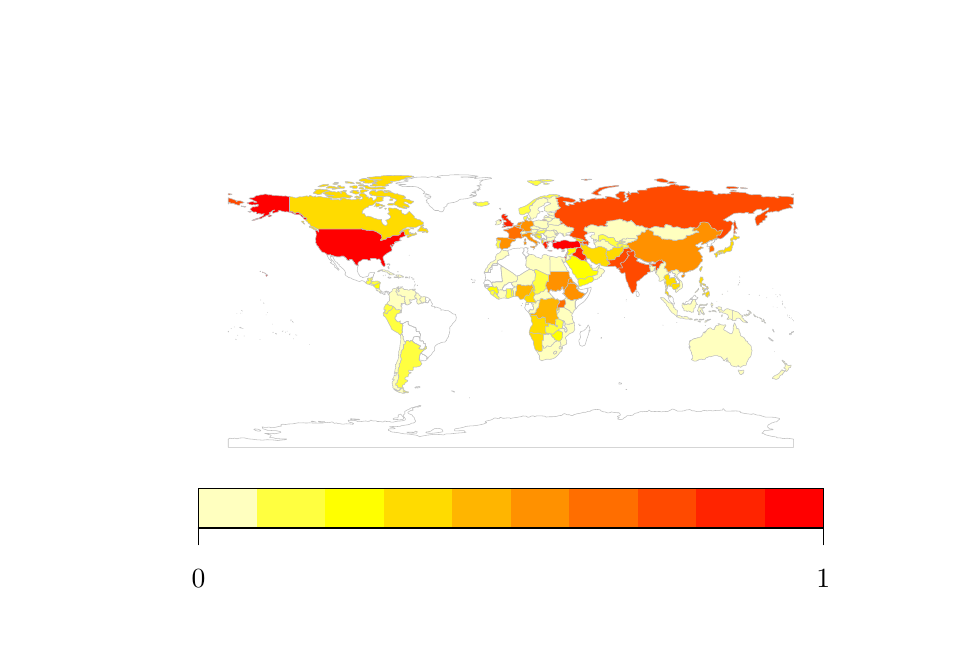
\begin{tikzpicture}[x=1pt,y=1pt]
\definecolor[named]{fillColor}{rgb}{1.00,1.00,1.00}
\path[use as bounding box,fill=fillColor,fill opacity=0.00] (0,0) rectangle (325.21,216.81);
\begin{scope}
\path[clip] ( 49.20, 61.20) rectangle (300.01,167.61);

\path[] ( 72.47, 65.14) rectangle (276.74,163.67);
\definecolor[named]{drawColor}{rgb}{0.75,0.75,0.75}

\path[draw=drawColor,line width= 0.2pt,line join=round,line cap=round] (141.35, 79.81) --
	(141.10, 79.68) --
	(140.68, 79.77) --
	(140.22, 79.72) --
	(139.83, 79.58) --
	(139.42, 79.44) --
	(139.14, 79.27) --
	(139.06, 79.05) --
	(139.09, 78.84) --
	(139.36, 78.65) --
	(138.97, 78.52) --
	(138.44, 78.47) --
	(138.13, 78.28) --
	(137.79, 78.11) --
	(137.44, 77.86) --
	(137.35, 77.65) --
	(137.55, 77.42) --
	(137.85, 77.24) --
	(138.32, 77.11) --
	(138.75, 76.93) --
	(138.98, 76.71) --
	(139.10, 76.49) --
	(139.27, 76.27) --
	(139.54, 76.08) --
	(139.70, 75.87) --
	(139.78, 75.35) --
	(139.95, 75.14) --
	(139.99, 74.92) --
	(140.17, 74.69) --
	(140.09, 74.39) --
	(139.78, 74.16) --
	(139.45, 73.97) --
	(138.69, 73.89) --
	(138.44, 73.69) --
	(138.09, 73.50) --
	(137.24, 73.29) --
	(136.48, 73.20) --
	(135.77, 73.08) --
	(135.00, 72.96) --
	(134.55, 72.72) --
	(133.64, 72.70) --
	(132.64, 72.72) --
	(131.74, 72.68) --
	(130.78, 72.68) --
	(130.96, 72.46) --
	(131.83, 72.36) --
	(132.46, 72.20) --
	(132.81, 72.00) --
	(132.18, 71.82) --
	(131.20, 71.88) --
	(130.39, 71.74) --
	(130.36, 71.50) --
	(130.34, 71.28) --
	(131.00, 71.09) --
	(131.13, 70.88) --
	(131.85, 70.67) --
	(133.05, 70.58) --
	(134.07, 70.42) --
	(134.88, 70.25) --
	(135.91, 70.07) --
	(137.33, 69.98) --
	(138.72, 69.82) --
	(139.68, 69.66) --
	(140.74, 69.47) --
	(141.29, 69.20) --
	(141.57, 68.99) --
	(142.26, 69.19) --
	(143.19, 69.36) --
	(144.18, 69.53) --
	(145.36, 69.68) --
	(146.37, 69.83) --
	(147.78, 69.85) --
	(149.17, 69.77) --
	(150.32, 69.63) --
	(150.68, 69.88) --
	(151.47, 70.05) --
	(152.91, 70.06) --
	(154.03, 70.18) --
	(155.10, 70.30) --
	(156.27, 70.38) --
	(157.53, 70.48) --
	(158.41, 70.62) --
	(158.01, 70.82) --
	(157.76, 71.02) --
	(157.76, 71.23) --
	(156.66, 71.21) --
	(155.50, 71.12) --
	(154.39, 71.12) --
	(154.23, 71.34) --
	(154.31, 71.76) --
	(154.56, 71.88) --
	(155.37, 72.01) --
	(156.33, 72.15) --
	(157.02, 72.31) --
	(157.71, 72.48) --
	(158.22, 72.70) --
	(159.00, 72.80) --
	(159.76, 72.88) --
	(160.15, 72.92) --
	(161.03, 72.95) --
	(161.86, 73.03) --
	(162.56, 73.14) --
	(163.25, 73.27) --
	(163.88, 73.40) --
	(164.66, 73.58) --
	(165.16, 73.77) --
	(165.70, 73.94) --
	(165.87, 74.16) --
	(165.26, 74.29) --
	(165.46, 74.53) --
	(165.84, 74.70) --
	(166.43, 74.82) --
	(167.05, 74.95) --
	(167.63, 75.13) --
	(168.08, 75.35) --
	(168.35, 75.62) --
	(168.77, 75.77) --
	(169.44, 75.74) --
	(169.72, 75.55) --
	(170.40, 75.53) --
	(170.42, 75.74) --
	(170.71, 75.96) --
	(171.32, 75.90) --
	(171.47, 75.69) --
	(172.14, 75.66) --
	(172.88, 75.76) --
	(173.59, 75.83) --
	(174.23, 75.79) --
	(174.48, 75.56) --
	(175.10, 75.75) --
	(175.68, 75.85) --
	(176.32, 75.93) --
	(176.96, 76.00) --
	(177.53, 76.14) --
	(178.17, 76.23) --
	(178.66, 76.35) --
	(179.00, 76.55) --
	(179.42, 76.41) --
	(180.01, 76.48) --
	(180.42, 76.22) --
	(180.75, 76.02) --
	(181.39, 76.13) --
	(181.65, 76.35) --
	(182.22, 76.51) --
	(182.97, 76.47) --
	(183.19, 76.26) --
	(183.66, 76.47) --
	(184.27, 76.54) --
	(184.94, 76.56) --
	(185.54, 76.55) --
	(186.17, 76.48) --
	(186.78, 76.45) --
	(187.05, 76.26) --
	(187.41, 76.09) --
	(188.04, 76.19) --
	(188.70, 76.22) --
	(189.35, 76.22) --
	(189.98, 76.23) --
	(190.55, 76.30) --
	(191.15, 76.37) --
	(191.65, 76.53) --
	(192.18, 76.63) --
	(192.76, 76.68) --
	(193.19, 76.84) --
	(193.50, 77.15) --
	(193.83, 77.34) --
	(194.41, 77.25) --
	(194.64, 77.05) --
	(195.13, 76.92) --
	(195.72, 76.96) --
	(196.12, 76.76) --
	(196.54, 76.62) --
	(197.12, 76.75) --
	(197.32, 76.99) --
	(197.83, 77.09) --
	(198.42, 77.28) --
	(198.97, 77.36) --
	(199.64, 77.47) --
	(200.08, 77.59) --
	(200.55, 77.73) --
	(200.99, 77.85) --
	(201.53, 77.78) --
	(202.04, 77.98) --
	(202.41, 78.14) --
	(202.94, 78.13) --
	(203.41, 78.26) --
	(203.52, 78.46) --
	(203.99, 78.62) --
	(204.46, 78.73) --
	(205.03, 78.82) --
	(205.55, 78.86) --
	(206.05, 78.83) --
	(206.58, 78.77) --
	(207.04, 78.62) --
	(207.10, 78.37) --
	(207.60, 78.18) --
	(207.94, 78.03) --
	(208.62, 77.96) --
	(209.00, 77.81) --
	(209.46, 77.65) --
	(210.01, 77.62) --
	(210.46, 77.73) --
	(210.95, 77.96) --
	(211.48, 77.84) --
	(212.04, 77.77) --
	(212.57, 77.71) --
	(213.13, 77.66) --
	(213.70, 77.66) --
	(214.16, 77.07) --
	(214.14, 76.93) --
	(214.07, 76.67) --
	(213.53, 76.53) --
	(213.09, 76.32) --
	(213.16, 76.09) --
	(213.80, 76.10) --
	(213.72, 75.88) --
	(213.43, 75.67) --
	(213.16, 75.44) --
	(213.60, 75.26) --
	(214.25, 75.20) --
	(214.91, 75.30) --
	(215.22, 75.53) --
	(215.41, 75.74) --
	(215.72, 75.92) --
	(216.07, 76.08) --
	(216.22, 76.28) --
	(216.52, 76.56) --
	(216.87, 76.62) --
	(217.52, 76.64) --
	(218.09, 76.71) --
	(218.66, 76.79) --
	(218.94, 77.02) --
	(219.11, 77.23) --
	(219.50, 77.44) --
	(220.05, 77.58) --
	(220.53, 77.69) --
	(220.84, 77.88) --
	(221.16, 77.98) --
	(221.58, 78.07) --
	(222.14, 78.02) --
	(222.65, 78.07) --
	(223.21, 78.14) --
	(223.83, 78.11) --
	(224.24, 78.26) --
	(224.53, 78.64) --
	(224.74, 78.48) --
	(225.01, 78.22) --
	(225.49, 78.11) --
	(226.03, 78.06) --
	(226.58, 78.13) --
	(227.15, 78.08) --
	(227.69, 78.07) --
	(228.04, 78.13) --
	(228.52, 78.09) --
	(228.95, 77.97) --
	(229.47, 78.05) --
	(230.08, 78.05) --
	(230.60, 78.13) --
	(231.19, 78.05) --
	(231.57, 78.24) --
	(231.86, 78.43) --
	(232.24, 78.58) --
	(232.96, 79.01) --
	(233.32, 78.93) --
	(233.76, 78.77) --
	(234.13, 78.57) --
	(234.86, 78.23) --
	(235.41, 78.22) --
	(235.93, 78.22) --
	(236.55, 78.28) --
	(237.16, 78.36) --
	(237.62, 78.52) --
	(238.01, 78.68) --
	(238.65, 78.71) --
	(239.07, 78.83) --
	(239.51, 78.72) --
	(239.80, 78.54) --
	(240.20, 78.36) --
	(240.82, 78.38) --
	(241.21, 78.24) --
	(241.89, 78.09) --
	(242.60, 78.04) --
	(243.19, 78.08) --
	(243.64, 78.26) --
	(244.01, 78.44) --
	(244.52, 78.48) --
	(245.04, 78.41) --
	(245.62, 78.35) --
	(246.16, 78.44) --
	(246.67, 78.44) --
	(247.17, 78.38) --
	(247.69, 78.33) --
	(248.20, 78.43) --
	(248.81, 78.52) --
	(249.39, 78.54) --
	(250.04, 78.54) --
	(250.56, 78.60) --
	(251.07, 78.64) --
	(251.23, 78.92) --
	(251.25, 79.15) --
	(251.60, 79.00) --
	(251.70, 78.74) --
	(251.89, 78.51) --
	(252.13, 78.32) --
	(252.60, 78.22) --
	(253.25, 78.25) --
	(253.99, 78.26) --
	(254.50, 78.30) --
	(255.25, 78.30) --
	(255.78, 78.31) --
	(256.53, 78.28) --
	(257.16, 78.24) --
	(257.56, 78.06) --
	(257.45, 77.85) --
	(257.82, 77.68) --
	(258.43, 77.55) --
	(259.06, 77.41) --
	(259.79, 77.31) --
	(260.56, 77.22) --
	(261.14, 77.13) --
	(261.78, 77.12) --
	(262.15, 77.31) --
	(262.65, 77.15) --
	(263.08, 76.97) --
	(263.58, 76.84) --
	(264.27, 76.78) --
	(264.93, 76.72) --
	(265.21, 76.49) --
	(265.85, 76.36) --
	(266.28, 76.16) --
	(266.92, 76.07) --
	(267.57, 76.08) --
	(268.18, 76.05) --
	(268.86, 76.06) --
	(269.54, 76.02) --
	(270.17, 75.94) --
	(270.76, 75.80) --
	(271.35, 75.69) --
	(271.75, 75.53) --
	(271.69, 75.30) --
	(271.38, 75.10) --
	(271.13, 74.85) --
	(270.93, 74.65) --
	(270.66, 74.41) --
	(269.92, 74.33) --
	(269.58, 74.13) --
	(268.85, 74.00) --
	(268.60, 73.78) --
	(268.21, 73.57) --
	(267.80, 73.39) --
	(267.56, 73.16) --
	(267.42, 72.95) --
	(267.36, 72.69) --
	(267.37, 72.48) --
	(267.70, 72.26) --
	(267.82, 72.05) --
	(268.08, 71.85) --
	(269.14, 71.77) --
	(269.36, 71.52) --
	(268.34, 71.44) --
	(267.47, 71.31) --
	(266.40, 71.29) --
	(265.92, 70.97) --
	(265.82, 70.70) --
	(265.57, 70.49) --
	(265.27, 70.28) --
	(266.03, 70.09) --
	(266.32, 69.86) --
	(266.81, 69.65) --
	(267.50, 69.46) --
	(268.28, 69.28) --
	(269.14, 69.10) --
	(270.44, 68.92) --
	(270.73, 68.64) --
	(272.36, 68.52) --
	(272.47, 68.48) --
	(272.90, 68.31) --
	(274.46, 68.46) --
	(275.76, 68.28) --
	(276.74, 68.14) --
	(276.74, 65.14) --
	( 72.47, 65.14) --
	( 72.47, 68.14) --
	( 72.51, 68.14) --
	( 73.01, 68.47) --
	( 74.03, 68.29) --
	( 74.10, 68.31) --
	( 74.70, 68.49) --
	( 74.77, 68.48) --
	( 74.84, 68.48) --
	( 75.66, 68.24) --
	( 76.38, 68.48) --
	( 76.51, 68.51) --
	( 78.18, 68.61) --
	( 78.72, 68.48) --
	( 78.98, 68.41) --
	( 79.84, 68.22) --
	( 81.45, 68.08) --
	( 82.73, 67.90) --
	( 84.92, 67.77) --
	( 86.55, 67.92) --
	( 88.96, 67.81) --
	( 90.33, 67.63) --
	( 91.83, 67.80) --
	( 93.41, 67.96) --
	( 93.53, 68.22) --
	( 91.30, 68.24) --
	( 89.46, 68.38) --
	( 88.98, 68.60) --
	( 87.46, 68.72) --
	( 87.56, 68.98) --
	( 87.77, 69.21) --
	( 87.98, 69.42) --
	( 87.87, 69.66) --
	( 86.93, 69.81) --
	( 86.49, 70.01) --
	( 85.62, 70.19) --
	( 86.99, 70.16) --
	( 88.31, 70.25) --
	( 89.13, 70.06) --
	( 90.14, 70.22) --
	( 91.07, 70.43) --
	( 91.53, 70.62) --
	( 91.33, 70.86) --
	( 90.60, 71.01) --
	( 89.76, 71.18) --
	( 88.59, 71.21) --
	( 87.57, 71.29) --
	( 86.47, 71.35) --
	( 86.11, 71.56) --
	( 85.37, 71.74) --
	( 84.93, 71.94) --
	( 84.75, 72.58) --
	( 85.03, 72.52) --
	( 85.54, 72.35) --
	( 86.47, 72.40) --
	( 87.37, 72.48) --
	( 87.84, 72.24) --
	( 88.74, 72.29) --
	( 89.50, 72.41) --
	( 90.21, 72.57) --
	( 90.85, 72.76) --
	( 91.71, 72.81) --
	( 91.68, 73.03) --
	( 91.48, 73.24) --
	( 91.65, 73.44) --
	( 92.38, 73.54) --
	( 92.72, 73.35) --
	( 93.58, 73.46) --
	( 94.24, 73.60) --
	( 95.05, 73.61) --
	( 95.82, 73.67) --
	( 96.59, 73.80) --
	( 97.20, 73.93) --
	( 97.89, 74.05) --
	( 98.33, 74.01) --
	( 98.72, 73.97) --
	( 99.56, 74.05) --
	(100.32, 73.95) --
	(101.10, 73.96) --
	(101.84, 74.04) --
	(102.61, 73.98) --
	(103.45, 73.93) --
	(104.24, 73.95) --
	(105.06, 73.94) --
	(105.91, 73.93) --
	(106.69, 73.95) --
	(107.27, 74.11) --
	(107.95, 74.20) --
	(108.67, 74.08) --
	(109.34, 74.18) --
	(109.95, 74.38) --
	(110.32, 74.20) --
	(110.52, 74.00) --
	(110.89, 73.81) --
	(111.48, 73.98) --
	(112.15, 73.77) --
	(112.92, 73.70) --
	(113.58, 73.55) --
	(114.38, 73.58) --
	(115.10, 73.68) --
	(115.96, 73.66) --
	(116.72, 73.58) --
	(117.50, 73.48) --
	(117.80, 73.73) --
	(117.43, 73.91) --
	(117.16, 74.11) --
	(116.42, 74.16) --
	(116.10, 74.37) --
	(115.98, 74.58) --
	(115.78, 75.00) --
	(116.21, 74.93) --
	(116.96, 74.89) --
	(117.69, 74.93) --
	(118.36, 74.84) --
	(118.93, 74.67) --
	(119.18, 74.47) --
	(119.95, 74.44) --
	(120.68, 74.51) --
	(121.46, 74.63) --
	(122.16, 74.69) --
	(122.73, 74.56) --
	(123.49, 74.60) --
	(123.98, 75.04) --
	(124.43, 74.78) --
	(125.09, 74.68) --
	(125.80, 74.74) --
	(126.27, 74.51) --
	(127.01, 74.49) --
	(127.70, 74.43) --
	(128.38, 74.30) --
	(128.82, 74.51) --
	(129.05, 74.72) --
	(129.61, 74.49) --
	(130.39, 74.55) --
	(130.97, 74.43) --
	(131.36, 74.24) --
	(132.11, 74.29) --
	(132.70, 74.41) --
	(133.28, 74.56) --
	(133.97, 74.64) --
	(134.77, 74.70) --
	(135.49, 74.78) --
	(136.05, 74.90) --
	(136.38, 75.08) --
	(136.52, 75.33) --
	(136.45, 75.56) --
	(136.27, 75.78) --
	(136.07, 76.00) --
	(135.89, 76.23) --
	(135.75, 76.43) --
	(135.71, 76.65) --
	(135.77, 76.87) --
	(136.04, 77.08) --
	(136.26, 77.32) --
	(136.35, 77.54) --
	(136.24, 77.78) --
	(136.17, 78.01) --
	(136.45, 78.26) --
	(136.76, 78.43) --
	(137.13, 78.64) --
	(137.52, 78.82) --
	(137.97, 78.98) --
	(138.19, 79.23) --
	(138.50, 79.38) --
	(138.86, 79.53) --
	(139.40, 79.56) --
	(139.76, 79.74) --
	(140.16, 79.85) --
	(140.63, 79.92) --
	(141.04, 80.06) --
	(141.36, 80.24) --
	(141.80, 80.31) --
	(142.14, 80.16) --
	(141.93, 79.97) --
	(141.35, 79.81) --
	(141.35, 79.81);

\path[draw=drawColor,line width= 0.2pt,line join=round,line cap=round] (148.99, 71.92) --
	(149.69, 71.68) --
	(149.93, 71.33) --
	(150.00, 71.09) --
	(150.02, 70.80) --
	(149.14, 70.62) --
	(148.22, 70.48) --
	(147.15, 70.34) --
	(145.96, 70.23) --
	(144.62, 70.27) --
	(143.87, 70.46) --
	(143.97, 70.69) --
	(145.19, 70.84) --
	(145.67, 71.03) --
	(146.03, 71.28) --
	(146.29, 71.49) --
	(146.63, 71.69) --
	(147.00, 71.92) --
	(147.00, 71.92) --
	(147.29, 71.92) --
	(148.13, 72.05) --
	(148.99, 71.92) --
	(148.99, 71.92);

\path[draw=drawColor,line width= 0.2pt,line join=round,line cap=round] (135.77, 75.95) --
	(135.83, 75.69) --
	(135.73, 75.47) --
	(135.58, 75.26) --
	(134.91, 75.18) --
	(134.28, 75.07) --
	(133.53, 75.08) --
	(133.81, 75.30) --
	(133.14, 75.22) --
	(132.51, 75.15) --
	(132.08, 75.31) --
	(132.04, 75.55) --
	(132.67, 75.77) --
	(132.67, 75.77) --
	(133.06, 75.84) --
	(133.71, 75.81) --
	(133.88, 76.10) --
	(133.91, 76.31) --
	(133.90, 76.77) --
	(134.22, 77.04) --
	(134.75, 77.13) --
	(135.05, 76.91) --
	(135.18, 76.70) --
	(135.42, 76.45) --
	(135.61, 76.20) --
	(135.77, 75.95) --
	(135.77, 75.95);

\path[draw=drawColor,line width= 0.2pt,line join=round,line cap=round] (140.81, 70.79) --
	(140.64, 70.50) --
	(140.47, 70.25) --
	(139.28, 70.33) --
	(138.02, 70.29) --
	(137.31, 70.48) --
	(137.31, 70.50) --
	(136.99, 70.67) --
	(138.27, 70.65) --
	(139.49, 70.59) --
	(139.92, 70.83) --
	(140.22, 71.03) --
	(140.81, 70.79) --
	(140.81, 70.79);

\path[draw=drawColor,line width= 0.2pt,line join=round,line cap=round] ( 84.27, 71.10) --
	( 83.18, 71.02) --
	( 82.44, 71.22) --
	( 82.10, 71.42) --
	( 82.08, 71.46) --
	( 81.72, 71.61) --
	( 81.72, 71.61) --
	( 82.06, 71.82) --
	( 83.12, 71.73) --
	( 83.68, 71.56) --
	( 84.12, 71.36) --
	( 84.27, 71.10) --
	( 84.27, 71.10);

\path[draw=drawColor,line width= 0.2pt,line join=round,line cap=round] (118.44, 75.39) --
	(119.07, 75.31) --
	(119.69, 75.38) --
	(120.02, 75.06) --
	(119.58, 75.10) --
	(118.89, 75.08) --
	(118.19, 75.10) --
	(117.42, 75.07) --
	(116.84, 75.18) --
	(116.54, 75.41) --
	(116.54, 75.41) --
	(116.90, 75.51) --
	(117.62, 75.44) --
	(118.44, 75.39) --
	(118.44, 75.39);

\path[draw=drawColor,line width= 0.2pt,line join=round,line cap=round] (105.83, 74.50) --
	(106.56, 74.41) --
	(107.24, 74.51) --
	(106.92, 74.31) --
	(106.39, 74.17) --
	(105.60, 74.21) --
	(105.03, 74.41) --
	(105.03, 74.41) --
	(105.15, 74.60) --
	(105.83, 74.50) --
	(105.83, 74.50);

\path[draw=drawColor,line width= 0.2pt,line join=round,line cap=round] (103.36, 74.51) --
	(104.23, 74.29) --
	(103.90, 74.31) --
	(103.16, 74.37) --
	(102.39, 74.53) --
	(102.39, 74.53) --
	(102.80, 74.65) --
	(103.36, 74.51) --
	(103.36, 74.51);
\definecolor[named]{fillColor}{rgb}{1.00,0.29,0.00}

\path[draw=drawColor,line width= 0.2pt,line join=round,line cap=round,fill=fillColor] (235.30,159.88) --
	(235.46,159.60) --
	(235.97,159.74) --
	(237.63,159.73) --
	(238.91,159.46) --
	(239.37,159.24) --
	(239.23,158.95) --
	(238.60,158.78) --
	(237.11,158.47) --
	(236.68,158.30) --
	(237.39,158.22) --
	(238.22,158.08) --
	(238.74,158.18) --
	(239.03,157.82) --
	(239.27,157.97) --
	(240.18,158.06) --
	(242.00,157.96) --
	(242.14,157.70) --
	(244.51,157.61) --
	(244.55,158.05) --
	(245.75,157.95) --
	(246.66,157.95) --
	(247.57,157.65) --
	(247.83,157.29) --
	(247.50,157.05) --
	(248.21,156.60) --
	(249.10,156.37) --
	(249.65,156.97) --
	(250.56,156.71) --
	(251.53,156.87) --
	(252.62,156.69) --
	(253.04,156.85) --
	(253.97,156.77) --
	(253.56,157.30) --
	(254.31,157.54) --
	(259.44,157.17) --
	(259.92,156.84) --
	(261.40,156.40) --
	(263.69,156.51) --
	(264.82,156.42) --
	(265.30,156.18) --
	(265.23,155.77) --
	(265.93,155.61) --
	(266.69,155.72) --
	(267.69,155.74) --
	(268.76,155.63) --
	(269.84,155.69) --
	(270.83,155.19) --
	(271.53,155.37) --
	(271.07,155.73) --
	(271.32,155.98) --
	(273.13,155.82) --
	(274.31,155.86) --
	(275.95,155.59) --
	(276.74,155.34) --
	(276.74,153.08) --
	(276.74,153.07) --
	(276.01,152.83) --
	(275.27,152.87) --
	(275.78,152.57) --
	(276.12,152.10) --
	(276.38,151.94) --
	(276.45,151.71) --
	(276.30,151.56) --
	(275.25,151.68) --
	(273.66,151.26) --
	(273.16,151.19) --
	(272.29,150.79) --
	(271.46,150.44) --
	(271.25,150.19) --
	(270.44,150.58) --
	(268.96,150.13) --
	(268.71,150.34) --
	(268.16,150.10) --
	(267.40,150.18) --
	(267.22,149.80) --
	(266.54,149.26) --
	(266.56,149.03) --
	(267.20,148.90) --
	(267.13,148.07) --
	(266.60,148.05) --
	(266.36,147.58) --
	(266.59,147.33) --
	(265.60,147.04) --
	(265.41,146.40) --
	(264.56,146.26) --
	(264.39,145.68) --
	(263.57,145.15) --
	(263.36,145.54) --
	(263.12,146.37) --
	(262.80,147.63) --
	(263.07,148.42) --
	(263.55,148.76) --
	(263.58,149.02) --
	(264.46,149.15) --
	(265.48,149.86) --
	(266.46,150.45) --
	(267.48,150.90) --
	(267.93,151.70) --
	(267.24,151.65) --
	(266.90,151.18) --
	(265.46,150.56) --
	(265.00,151.26) --
	(263.53,151.07) --
	(262.11,150.12) --
	(262.58,149.77) --
	(261.31,149.62) --
	(260.44,149.56) --
	(260.48,149.97) --
	(259.60,150.06) --
	(258.89,149.78) --
	(257.16,149.88) --
	(255.29,149.71) --
	(253.45,148.60) --
	(251.28,147.26) --
	(252.17,147.19) --
	(252.45,146.84) --
	(253.00,146.71) --
	(253.37,146.99) --
	(253.99,146.96) --
	(254.81,146.33) --
	(254.83,145.85) --
	(254.38,145.28) --
	(254.34,144.60) --
	(254.08,143.70) --
	(253.22,142.88) --
	(253.03,142.48) --
	(252.26,141.82) --
	(251.50,141.17) --
	(251.13,140.83) --
	(250.38,140.50) --
	(250.02,140.49) --
	(249.66,140.77) --
	(248.90,140.35) --
	(248.81,140.16) --
	(248.73,140.26) --
	(248.73,140.55) --
	(249.02,140.57) --
	(249.10,141.24) --
	(248.95,141.72) --
	(249.44,141.92) --
	(250.13,141.82) --
	(250.51,142.38) --
	(250.70,143.00) --
	(250.92,143.20) --
	(251.22,143.71) --
	(250.28,143.55) --
	(249.79,143.32) --
	(248.93,143.32) --
	(248.70,143.86) --
	(248.03,144.26) --
	(247.04,144.44) --
	(246.83,145.00) --
	(246.63,145.35) --
	(246.42,145.59) --
	(246.07,146.16) --
	(245.57,146.37) --
	(244.72,146.54) --
	(243.97,146.53) --
	(243.27,146.42) --
	(242.80,146.14) --
	(243.11,146.01) --
	(243.12,145.69) --
	(242.80,145.51) --
	(242.29,144.91) --
	(242.29,144.66) --
	(241.49,144.30) --
	(240.81,144.52) --
	(240.14,144.47) --
	(239.84,144.66) --
	(239.50,144.72) --
	(238.67,144.32) --
	(237.92,144.23) --
	(237.40,144.08) --
	(236.68,144.18) --
	(236.16,144.17) --
	(235.81,144.46) --
	(235.26,144.73) --
	(234.69,144.81) --
	(233.97,144.73) --
	(233.43,144.63) --
	(232.63,144.87) --
	(232.52,145.29) --
	(231.85,145.44) --
	(231.34,145.51) --
	(230.70,145.74) --
	(230.11,145.15) --
	(230.35,144.82) --
	(229.79,144.42) --
	(228.97,144.57) --
	(228.41,144.59) --
	(228.03,144.85) --
	(227.44,144.86) --
	(226.94,145.03) --
	(226.08,144.77) --
	(225.00,144.28) --
	(224.40,144.18) --
	(224.18,144.13) --
	(223.88,144.48) --
	(223.14,144.40) --
	(222.90,144.64) --
	(222.51,144.76) --
	(222.23,145.08) --
	(221.92,145.19) --
	(221.10,145.04) --
	(220.32,145.37) --
	(220.02,145.07) --
	(218.75,146.51) --
	(218.03,146.95) --
	(218.24,147.13) --
	(216.81,146.59) --
	(216.27,146.56) --
	(216.32,146.87) --
	(215.59,147.06) --
	(215.00,146.92) --
	(214.82,147.51) --
	(213.80,147.63) --
	(213.29,147.40) --
	(211.87,147.19) --
	(211.59,147.05) --
	(209.47,146.85) --
	(209.21,146.66) --
	(209.62,146.27) --
	(209.07,146.12) --
	(209.18,145.97) --
	(208.63,145.69) --
	(209.55,145.30) --
	(209.41,145.03) --
	(208.61,145.06) --
	(208.45,144.89) --
	(207.72,145.18) --
	(206.82,145.17) --
	(206.22,144.93) --
	(205.55,145.16) --
	(204.30,145.55) --
	(203.41,145.54) --
	(202.24,144.92) --
	(202.17,144.51) --
	(201.59,144.84) --
	(201.13,144.21) --
	(201.30,144.10) --
	(200.97,143.67) --
	(201.45,143.28) --
	(201.88,143.30) --
	(202.24,142.92) --
	(202.18,142.63) --
	(202.47,142.54) --
	(202.21,142.20) --
	(201.66,142.11) --
	(201.10,141.52) --
	(201.61,140.98) --
	(201.56,140.60) --
	(202.17,139.93) --
	(201.84,139.70) --
	(201.74,139.56) --
	(201.49,139.60) --
	(201.10,139.94) --
	(200.94,139.96) --
	(200.58,140.09) --
	(200.41,140.32) --
	(199.88,140.44) --
	(199.53,140.35) --
	(199.44,140.46) --
	(198.66,140.73) --
	(197.83,140.82) --
	(197.35,140.92) --
	(197.28,140.85) --
	(196.55,141.33) --
	(195.91,141.55) --
	(195.42,141.88) --
	(195.83,141.97) --
	(196.30,142.45) --
	(195.98,142.67) --
	(196.82,142.90) --
	(196.81,143.03) --
	(196.30,142.93) --
	(196.31,143.19) --
	(196.61,143.34) --
	(197.16,143.39) --
	(197.24,143.58) --
	(197.12,143.89) --
	(197.35,144.19) --
	(197.34,144.35) --
	(196.51,144.54) --
	(196.18,144.53) --
	(195.82,144.80) --
	(195.39,144.71) --
	(194.67,144.91) --
	(194.68,145.02) --
	(194.48,145.26) --
	(194.03,145.29) --
	(193.98,145.47) --
	(194.12,145.58) --
	(193.76,145.90) --
	(193.17,145.85) --
	(193.00,145.88) --
	(192.86,145.75) --
	(192.64,145.77) --
	(192.50,146.13) --
	(192.37,146.32) --
	(192.48,146.38) --
	(192.94,146.36) --
	(193.16,146.48) --
	(192.99,146.63) --
	(192.61,146.73) --
	(192.65,146.83) --
	(192.42,146.94) --
	(192.06,147.31) --
	(192.18,147.46) --
	(192.13,147.73) --
	(191.57,147.86) --
	(191.27,147.80) --
	(191.19,147.94) --
	(190.60,148.08) --
	(190.41,148.41) --
	(190.36,148.69) --
	(190.09,148.82) --
	(190.33,149.00) --
	(190.17,149.53) --
	(190.57,149.86) --
	(190.48,149.95) --
	(191.13,150.27) --
	(190.53,150.54) --
	(191.75,151.26) --
	(192.28,151.59) --
	(192.49,151.88) --
	(191.65,152.27) --
	(191.88,152.64) --
	(191.37,153.06) --
	(191.75,153.55) --
	(191.09,154.19) --
	(191.62,154.62) --
	(190.75,155.00) --
	(190.83,155.40) --
	(191.29,155.45) --
	(192.25,155.68) --
	(192.84,155.87) --
	(193.77,155.53) --
	(195.33,155.40) --
	(197.47,154.75) --
	(197.91,154.48) --
	(197.94,154.11) --
	(197.31,153.81) --
	(196.39,153.66) --
	(193.85,154.09) --
	(193.44,154.02) --
	(194.36,153.60) --
	(194.40,153.34) --
	(194.43,152.76) --
	(195.17,152.58) --
	(195.61,152.44) --
	(195.68,152.71) --
	(195.34,152.96) --
	(195.70,153.17) --
	(197.07,152.82) --
	(197.55,152.96) --
	(197.17,153.37) --
	(198.49,153.93) --
	(199.02,153.89) --
	(199.54,153.70) --
	(199.88,154.09) --
	(199.40,154.42) --
	(199.68,154.76) --
	(199.26,155.12) --
	(200.85,154.93) --
	(201.17,154.62) --
	(200.46,154.55) --
	(200.46,154.23) --
	(200.91,154.04) --
	(201.78,154.16) --
	(201.92,154.52) --
	(203.11,154.79) --
	(205.09,155.28) --
	(205.52,155.25) --
	(204.96,154.91) --
	(205.66,154.85) --
	(206.07,155.04) --
	(207.13,155.06) --
	(207.97,155.29) --
	(208.62,154.95) --
	(209.26,155.33) --
	(208.67,155.65) --
	(208.96,155.84) --
	(210.64,155.67) --
	(211.43,155.49) --
	(213.48,154.84) --
	(213.86,155.14) --
	(213.28,155.44) --
	(213.27,155.56) --
	(212.58,155.62) --
	(212.77,155.89) --
	(212.47,156.33) --
	(212.45,156.51) --
	(213.50,157.02) --
	(213.87,157.54) --
	(214.29,157.65) --
	(215.79,157.50) --
	(215.91,157.19) --
	(215.37,156.73) --
	(215.73,156.55) --
	(215.91,156.15) --
	(215.78,155.37) --
	(216.41,155.02) --
	(216.16,154.64) --
	(215.05,153.84) --
	(215.70,153.75) --
	(215.93,153.96) --
	(216.55,154.10) --
	(216.70,154.39) --
	(217.19,154.66) --
	(216.86,154.98) --
	(217.13,155.35) --
	(216.51,155.40) --
	(216.37,155.72) --
	(216.82,156.28) --
	(216.09,156.75) --
	(217.10,157.13) --
	(216.97,157.53) --
	(217.25,157.55) --
	(217.55,157.23) --
	(217.33,156.68) --
	(217.93,156.58) --
	(217.68,156.99) --
	(218.63,157.21) --
	(219.80,157.24) --
	(220.85,156.92) --
	(220.35,157.39) --
	(220.29,158.00) --
	(221.28,158.11) --
	(222.64,158.09) --
	(223.87,158.16) --
	(223.41,158.46) --
	(224.07,158.83) --
	(224.72,158.85) --
	(225.82,159.13) --
	(227.32,159.20) --
	(227.51,159.36) --
	(229.00,159.41) --
	(229.46,159.28) --
	(230.74,159.58) --
	(231.78,159.58) --
	(231.94,159.82) --
	(232.48,160.06) --
	(233.82,160.29) --
	(234.79,160.11) --
	(234.02,159.97) --
	(235.30,159.88) --
	cycle;

\path[draw=drawColor,line width= 0.2pt,line join=round,line cap=round,fill=fillColor] (207.25,156.34) --
	(206.92,156.29) --
	(205.06,156.36) --
	(204.91,156.61) --
	(203.89,156.76) --
	(203.80,157.07) --
	(204.38,157.19) --
	(204.36,157.50) --
	(205.49,157.98) --
	(204.97,158.05) --
	(206.33,158.55) --
	(206.17,158.81) --
	(207.44,159.11) --
	(209.32,159.47) --
	(211.20,159.58) --
	(212.18,159.79) --
	(213.28,159.86) --
	(213.67,159.64) --
	(213.29,159.46) --
	(211.28,159.18) --
	(209.55,158.91) --
	(207.79,158.37) --
	(206.94,157.82) --
	(206.05,157.27) --
	(206.17,156.80) --
	(207.25,156.34) --
	cycle;

\path[draw=drawColor,line width= 0.2pt,line join=round,line cap=round,fill=fillColor] ( 75.30,153.99) --
	( 75.69,153.85) --
	( 75.55,154.26) --
	( 77.09,154.17) --
	( 78.20,153.64) --
	( 77.64,153.40) --
	( 76.71,153.34) --
	( 76.70,152.78) --
	( 76.47,152.67) --
	( 75.94,152.68) --
	( 75.51,152.88) --
	( 74.75,153.05) --
	( 74.63,153.29) --
	( 74.05,153.38) --
	( 73.40,153.31) --
	( 73.10,153.51) --
	( 73.22,153.72) --
	( 72.54,153.59) --
	( 72.80,153.32) --
	( 72.47,153.08) --
	( 72.47,155.34) --
	( 73.86,154.91) --
	( 75.35,154.34) --
	( 75.30,153.99) --
	cycle;

\path[draw=drawColor,line width= 0.2pt,line join=round,line cap=round,fill=fillColor] (231.31,160.97) --
	(230.08,160.89) --
	(228.50,161.06) --
	(227.55,161.28) --
	(227.12,161.68) --
	(226.34,161.79) --
	(227.82,162.18) --
	(229.05,162.31) --
	(230.15,162.02) --
	(231.45,161.48) --
	(231.31,160.97) --
	cycle;

\path[draw=drawColor,line width= 0.2pt,line join=round,line cap=round,fill=fillColor] (256.11,145.00) --
	(256.69,144.00) --
	(255.85,144.18) --
	(255.50,143.36) --
	(256.05,142.78) --
	(256.03,142.39) --
	(255.60,142.73) --
	(255.23,142.29) --
	(255.13,142.77) --
	(255.19,143.32) --
	(255.13,143.93) --
	(255.26,144.36) --
	(255.28,145.12) --
	(254.95,145.68) --
	(255.00,146.45) --
	(255.52,146.71) --
	(255.30,146.98) --
	(255.55,147.06) --
	(255.70,146.68) --
	(255.89,146.13) --
	(255.88,145.58) --
	(256.11,145.00) --
	cycle;

\path[draw=drawColor,line width= 0.2pt,line join=round,line cap=round,fill=fillColor] (256.93,159.08) --
	(256.48,158.66) --
	(254.39,158.68) --
	(253.45,158.54) --
	(252.33,158.91) --
	(252.63,159.30) --
	(253.38,159.41) --
	(254.88,159.38) --
	(256.93,159.08) --
	cycle;

\path[draw=drawColor,line width= 0.2pt,line join=round,line cap=round,fill=fillColor] (234.23,160.64) --
	(231.03,160.42) --
	(232.07,161.17) --
	(232.53,161.23) --
	(232.96,161.19) --
	(234.40,160.87) --
	(234.23,160.64) --
	cycle;

\path[draw=drawColor,line width= 0.2pt,line join=round,line cap=round,fill=fillColor] (203.62,161.91) --
	(202.86,161.84) --
	(202.35,161.79) --
	(202.27,161.70) --
	(201.61,161.61) --
	(200.99,161.74) --
	(201.32,161.92) --
	(200.05,161.94) --
	(201.16,162.04) --
	(202.02,162.05) --
	(202.14,161.89) --
	(202.47,162.03) --
	(203.00,162.12) --
	(203.84,162.00) --
	(203.62,161.91) --
	cycle;

\path[draw=drawColor,line width= 0.2pt,line join=round,line cap=round,fill=fillColor] (187.51,147.03) --
	(186.46,147.03) --
	(185.76,147.09) --
	(185.89,147.34) --
	(186.68,147.52) --
	(187.27,147.42) --
	(187.52,147.33) --
	(187.46,147.18) --
	(187.51,147.03) --
	cycle;

\path[draw=drawColor,line width= 0.2pt,line join=round,line cap=round,fill=fillColor] (260.13,158.81) --
	(259.48,158.59) --
	(258.57,158.64) --
	(257.52,158.86) --
	(257.65,159.05) --
	(258.71,158.96) --
	(260.13,158.81) --
	cycle;

\path[draw=drawColor,line width= 0.2pt,line join=round,line cap=round,fill=fillColor] (256.09,157.75) --
	(255.23,157.75) --
	(254.07,157.81) --
	(253.97,157.84) --
	(254.51,158.06) --
	(255.21,158.12) --
	(256.02,157.90) --
	(256.09,157.75) --
	cycle;

\path[draw=drawColor,line width= 0.2pt,line join=round,line cap=round,fill=fillColor] ( 73.22,156.43) --
	( 72.47,156.40) --
	( 72.47,156.79) --
	( 72.55,156.81) --
	( 73.03,156.81) --
	( 73.85,156.65) --
	( 73.80,156.57) --
	( 73.22,156.43) --
	cycle;

\path[draw=drawColor,line width= 0.2pt,line join=round,line cap=round,fill=fillColor] (276.74,156.40) --
	(276.12,156.37) --
	(276.02,156.55) --
	(276.74,156.79) --
	(276.74,156.40) --
	cycle;
\definecolor[named]{fillColor}{rgb}{1.00,0.86,0.00}

\path[draw=drawColor,line width= 0.2pt,line join=round,line cap=round,fill=fillColor] (123.23,155.64) --
	(123.23,155.06) --
	(123.99,155.51) --
	(124.66,155.14) --
	(124.50,154.72) --
	(125.04,154.34) --
	(125.64,154.75) --
	(126.05,155.24) --
	(126.08,155.86) --
	(126.89,155.82) --
	(127.73,155.73) --
	(128.49,155.45) --
	(128.52,155.17) --
	(128.10,154.87) --
	(128.50,154.56) --
	(128.43,154.29) --
	(127.32,153.89) --
	(126.53,153.80) --
	(125.94,153.97) --
	(125.77,153.69) --
	(125.23,153.21) --
	(125.06,152.96) --
	(124.40,152.58) --
	(123.59,152.54) --
	(123.14,152.30) --
	(123.10,151.93) --
	(122.44,151.86) --
	(121.75,151.40) --
	(121.13,150.76) --
	(120.91,150.31) --
	(120.88,149.66) --
	(121.72,149.56) --
	(121.97,149.03) --
	(122.24,148.60) --
	(123.03,148.71) --
	(124.09,148.47) --
	(124.65,148.25) --
	(125.06,147.98) --
	(125.77,147.83) --
	(126.37,147.59) --
	(127.31,147.55) --
	(127.93,147.50) --
	(127.83,147.01) --
	(128.01,146.44) --
	(128.42,145.80) --
	(129.26,145.26) --
	(129.70,145.45) --
	(130.01,146.03) --
	(129.71,146.93) --
	(129.31,147.23) --
	(130.22,147.49) --
	(130.86,147.89) --
	(131.18,148.29) --
	(131.13,148.67) --
	(130.75,149.15) --
	(130.06,149.57) --
	(130.73,150.17) --
	(130.48,150.68) --
	(130.29,151.57) --
	(130.68,151.70) --
	(131.66,151.55) --
	(132.24,151.49) --
	(132.71,151.64) --
	(133.24,151.45) --
	(133.94,151.12) --
	(134.11,150.90) --
	(135.12,150.85) --
	(135.10,150.38) --
	(135.29,149.66) --
	(135.81,149.57) --
	(136.22,149.24) --
	(137.04,149.55) --
	(137.59,150.18) --
	(137.96,150.44) --
	(138.40,149.94) --
	(139.14,149.21) --
	(139.77,148.53) --
	(139.54,148.18) --
	(140.30,147.86) --
	(140.81,147.53) --
	(141.71,147.38) --
	(142.08,147.20) --
	(142.30,146.72) --
	(142.74,146.65) --
	(142.97,146.43) --
	(143.01,145.80) --
	(142.60,145.58) --
	(142.19,145.38) --
	(141.26,145.18) --
	(140.54,144.72) --
	(139.58,144.62) --
	(138.37,144.74) --
	(137.52,144.75) --
	(136.93,144.71) --
	(136.46,144.30) --
	(135.73,144.05) --
	(134.92,143.30) --
	(134.26,142.77) --
	(134.74,142.87) --
	(135.65,143.61) --
	(136.85,144.09) --
	(137.69,144.14) --
	(138.20,143.86) --
	(137.66,143.48) --
	(137.84,142.87) --
	(138.03,142.44) --
	(138.76,142.16) --
	(139.70,142.24) --
	(140.27,142.88) --
	(140.31,142.47) --
	(140.67,142.26) --
	(139.97,141.89) --
	(138.72,141.55) --
	(138.15,141.32) --
	(137.52,140.92) --
	(137.09,140.96) --
	(137.07,141.44) --
	(138.05,141.91) --
	(137.14,141.89) --
	(136.51,141.82) --
	(136.14,142.14) --
	(136.14,142.91) --
	(135.89,143.08) --
	(135.51,142.98) --
	(135.32,143.13) --
	(134.89,142.70) --
	(134.72,142.26) --
	(134.51,142.00) --
	(134.27,141.91) --
	(134.09,141.89) --
	(134.03,141.75) --
	(132.99,141.75) --
	(132.13,141.74) --
	(131.87,141.64) --
	(131.27,141.23) --
	(131.20,141.18) --
	(131.02,140.96) --
	(130.50,140.96) --
	(129.94,140.96) --
	(129.68,140.87) --
	(129.78,140.76) --
	(129.83,140.59) --
	(129.82,140.53) --
	(129.07,140.25) --
	(128.49,140.16) --
	(127.83,139.85) --
	(127.69,139.85) --
	(127.50,139.94) --
	(127.43,140.03) --
	(127.44,140.08) --
	(127.57,140.28) --
	(127.84,140.60) --
	(128.00,140.93) --
	(127.89,141.42) --
	(127.77,141.94) --
	(127.18,142.20) --
	(127.25,142.31) --
	(127.16,142.38) --
	(127.01,142.38) --
	(126.89,142.46) --
	(126.86,142.60) --
	(126.75,142.54) --
	(126.60,142.56) --
	(126.64,142.61) --
	(126.50,142.67) --
	(126.45,142.82) --
	(126.01,143.00) --
	(125.55,143.19) --
	(124.99,143.41) --
	(124.46,143.62) --
	(123.95,143.45) --
	(123.77,143.45) --
	(123.07,143.60) --
	(122.61,143.52) --
	(122.06,143.70) --
	(121.48,143.79) --
	(121.08,143.82) --
	(120.91,143.92) --
	(120.81,144.23) --
	(120.62,144.23) --
	(120.61,144.01) --
	(119.44,144.01) --
	(117.50,144.01) --
	(115.57,144.01) --
	(113.87,144.01) --
	(112.16,144.01) --
	(110.49,144.01) --
	(108.76,144.01) --
	(108.20,144.01) --
	(106.52,144.01) --
	(104.91,144.01) --
	(104.83,144.01) --
	(103.73,144.57) --
	(103.33,144.81) --
	(102.30,145.05) --
	(101.98,145.55) --
	(102.06,145.90) --
	(101.34,146.14) --
	(101.24,146.60) --
	(100.55,147.01) --
	(100.54,147.30) --
	(100.86,147.58) --
	(100.84,147.94) --
	( 99.88,148.30) --
	( 99.30,148.94) --
	( 98.94,149.35) --
	( 98.42,149.61) --
	( 98.04,149.84) --
	( 97.74,150.13) --
	( 97.17,149.95) --
	( 96.62,149.63) --
	( 96.11,150.00) --
	( 95.72,150.25) --
	( 95.16,150.41) --
	( 94.60,150.43) --
	( 94.61,153.66) --
	( 94.61,155.76) --
	( 95.67,155.63) --
	( 96.56,155.35) --
	( 97.15,155.30) --
	( 97.65,155.54) --
	( 98.34,155.72) --
	( 99.18,155.65) --
	(100.03,155.90) --
	(100.96,156.04) --
	(101.35,155.80) --
	(101.77,155.93) --
	(101.90,156.20) --
	(102.29,156.14) --
	(103.25,155.63) --
	(104.01,156.02) --
	(104.08,155.59) --
	(104.78,155.68) --
	(105.00,155.84) --
	(105.68,155.81) --
	(106.55,155.57) --
	(107.88,155.37) --
	(108.66,155.27) --
	(109.22,155.31) --
	(109.98,155.02) --
	(109.18,154.74) --
	(110.21,154.61) --
	(111.74,154.68) --
	(112.22,154.78) --
	(112.83,154.44) --
	(113.45,154.73) --
	(112.87,154.97) --
	(113.23,155.16) --
	(113.92,155.19) --
	(114.38,155.25) --
	(114.84,155.11) --
	(115.41,154.80) --
	(116.04,154.85) --
	(117.04,154.59) --
	(117.92,154.68) --
	(118.75,154.67) --
	(118.68,155.02) --
	(119.19,155.12) --
	(120.07,154.93) --
	(120.06,154.39) --
	(120.43,154.84) --
	(120.88,154.83) --
	(121.14,155.40) --
	(120.53,155.75) --
	(119.87,155.98) --
	(119.91,156.60) --
	(120.59,157.02) --
	(121.33,156.93) --
	(121.91,156.67) --
	(122.68,156.04) --
	(122.17,155.76) --
	(123.23,155.64) --
	cycle;

\path[draw=drawColor,line width= 0.2pt,line join=round,line cap=round,fill=fillColor] (125.49,157.72) --
	(125.94,157.36) --
	(126.46,157.82) --
	(127.90,158.05) --
	(128.87,157.47) --
	(128.79,157.10) --
	(129.91,157.26) --
	(130.45,157.49) --
	(131.71,157.20) --
	(132.49,156.93) --
	(132.56,156.68) --
	(133.62,156.81) --
	(134.21,156.45) --
	(135.58,156.22) --
	(136.07,156.00) --
	(136.61,155.46) --
	(135.57,155.20) --
	(136.90,154.83) --
	(137.80,154.71) --
	(138.62,154.18) --
	(139.51,154.15) --
	(139.34,153.75) --
	(138.34,153.09) --
	(137.64,153.33) --
	(136.75,153.88) --
	(136.02,153.81) --
	(135.94,153.48) --
	(136.54,153.15) --
	(137.31,152.89) --
	(137.54,152.74) --
	(137.91,152.18) --
	(137.72,151.77) --
	(137.00,151.92) --
	(135.58,152.38) --
	(136.38,151.89) --
	(136.97,151.55) --
	(137.06,151.35) --
	(135.53,151.57) --
	(134.31,151.90) --
	(133.62,152.18) --
	(133.82,152.34) --
	(132.97,152.63) --
	(132.15,152.91) --
	(132.15,152.74) --
	(130.51,152.65) --
	(130.03,152.85) --
	(130.41,153.26) --
	(131.47,153.28) --
	(132.64,153.35) --
	(132.45,153.55) --
	(132.65,153.83) --
	(133.38,154.39) --
	(133.23,154.64) --
	(133.01,154.83) --
	(132.14,155.11) --
	(130.99,155.30) --
	(131.35,155.44) --
	(130.75,155.80) --
	(130.25,155.83) --
	(129.81,156.02) --
	(129.50,155.85) --
	(128.47,155.78) --
	(126.41,155.91) --
	(125.21,156.07) --
	(124.29,156.16) --
	(123.82,156.36) --
	(124.41,156.62) --
	(123.60,156.62) --
	(123.42,157.19) --
	(123.86,157.70) --
	(124.44,157.93) --
	(125.91,158.08) --
	(125.49,157.72) --
	cycle;

\path[draw=drawColor,line width= 0.2pt,line join=round,line cap=round,fill=fillColor] (135.74,163.36) --
	(137.26,163.32) --
	(138.47,163.25) --
	(139.51,163.09) --
	(139.49,162.94) --
	(138.10,162.69) --
	(136.73,162.58) --
	(136.22,162.45) --
	(137.45,162.46) --
	(136.11,162.11) --
	(135.19,161.95) --
	(134.22,161.49) --
	(133.05,161.39) --
	(132.69,161.28) --
	(130.97,161.22) --
	(131.75,161.15) --
	(131.36,161.04) --
	(131.83,160.76) --
	(131.29,160.57) --
	(130.41,160.41) --
	(130.14,160.19) --
	(129.35,160.02) --
	(129.43,159.89) --
	(130.40,159.91) --
	(130.41,159.77) --
	(128.90,159.43) --
	(127.41,159.59) --
	(125.75,159.50) --
	(124.90,159.57) --
	(123.83,159.60) --
	(123.76,159.87) --
	(124.81,160.00) --
	(124.53,160.41) --
	(124.87,160.45) --
	(126.39,160.20) --
	(125.62,160.57) --
	(124.70,160.68) --
	(125.16,160.90) --
	(126.16,161.03) --
	(126.32,161.23) --
	(125.52,161.45) --
	(125.28,161.74) --
	(126.83,161.72) --
	(127.28,161.66) --
	(128.17,161.86) --
	(126.89,161.93) --
	(124.90,161.89) --
	(123.90,162.09) --
	(123.43,162.32) --
	(122.76,162.48) --
	(122.64,162.68) --
	(123.48,162.78) --
	(124.15,162.80) --
	(125.26,162.89) --
	(126.09,163.11) --
	(126.80,163.08) --
	(127.41,162.92) --
	(127.84,163.22) --
	(128.59,163.31) --
	(129.61,163.38) --
	(131.34,163.40) --
	(131.64,163.34) --
	(133.28,163.44) --
	(134.51,163.40) --
	(135.74,163.36) --
	cycle;

\path[draw=drawColor,line width= 0.2pt,line join=round,line cap=round,fill=fillColor] (109.83,157.70) --
	(109.54,157.43) --
	(110.81,157.60) --
	(111.60,157.32) --
	(112.24,157.61) --
	(112.76,157.42) --
	(113.22,156.86) --
	(113.51,157.10) --
	(113.10,157.68) --
	(113.60,157.76) --
	(114.17,157.67) --
	(114.80,157.44) --
	(115.16,156.89) --
	(115.33,156.49) --
	(116.29,156.21) --
	(117.31,155.94) --
	(117.25,155.69) --
	(116.32,155.65) --
	(116.68,155.43) --
	(116.49,155.22) --
	(115.46,155.31) --
	(114.48,155.46) --
	(113.83,155.43) --
	(112.76,155.23) --
	(111.32,155.15) --
	(110.31,155.10) --
	(110.01,155.36) --
	(109.23,155.52) --
	(108.73,155.45) --
	(108.03,155.90) --
	(108.41,155.96) --
	(109.28,156.06) --
	(110.08,156.04) --
	(110.82,156.13) --
	(109.72,156.27) --
	(108.51,156.22) --
	(107.71,156.23) --
	(107.41,156.44) --
	(108.72,156.67) --
	(107.85,156.66) --
	(106.86,156.81) --
	(107.33,157.24) --
	(107.73,157.46) --
	(109.25,157.81) --
	(109.83,157.70) --
	cycle;

\path[draw=drawColor,line width= 0.2pt,line join=round,line cap=round,fill=fillColor] (106.26,156.71) --
	(104.76,156.44) --
	(104.46,156.69) --
	(103.15,156.99) --
	(103.40,157.23) --
	(103.79,157.64) --
	(104.28,158.01) --
	(103.73,158.36) --
	(105.65,158.45) --
	(106.46,158.33) --
	(107.91,158.30) --
	(108.46,158.14) --
	(109.07,157.90) --
	(108.35,157.76) --
	(106.96,157.36) --
	(106.26,156.96) --
	(106.26,156.71) --
	cycle;

\path[draw=drawColor,line width= 0.2pt,line join=round,line cap=round,fill=fillColor] (125.23,161.41) --
	(125.92,161.22) --
	(125.14,161.06) --
	(124.09,160.63) --
	(123.08,160.59) --
	(121.91,160.66) --
	(121.30,160.89) --
	(121.31,161.10) --
	(121.76,161.25) --
	(120.72,161.24) --
	(120.09,161.43) --
	(119.73,161.69) --
	(120.13,161.94) --
	(120.52,162.12) --
	(121.10,162.16) --
	(120.85,162.29) --
	(122.17,162.31) --
	(122.90,162.01) --
	(123.85,161.89) --
	(124.78,161.78) --
	(125.23,161.41) --
	cycle;

\path[draw=drawColor,line width= 0.2pt,line join=round,line cap=round,fill=fillColor] (120.88,159.95) --
	(121.51,159.77) --
	(122.63,159.77) --
	(123.12,159.59) --
	(122.99,159.37) --
	(123.64,159.24) --
	(124.00,159.11) --
	(124.77,159.08) --
	(125.60,159.04) --
	(126.50,159.16) --
	(127.65,159.21) --
	(128.57,159.17) --
	(129.18,158.95) --
	(129.31,158.72) --
	(128.96,158.57) --
	(128.11,158.45) --
	(127.38,158.52) --
	(125.76,158.43) --
	(124.59,158.42) --
	(123.67,158.49) --
	(122.17,158.67) --
	(121.97,158.98) --
	(121.90,159.26) --
	(121.33,159.51) --
	(120.16,159.58) --
	(119.50,159.76) --
	(119.71,159.99) --
	(120.88,159.95) --
	cycle;

\path[draw=drawColor,line width= 0.2pt,line join=round,line cap=round,fill=fillColor] (142.76,144.97) --
	(142.38,144.47) --
	(142.75,144.66) --
	(143.13,144.54) --
	(142.93,144.34) --
	(143.44,144.19) --
	(143.70,144.33) --
	(144.26,144.15) --
	(144.09,143.74) --
	(144.49,143.83) --
	(144.56,143.53) --
	(144.73,143.18) --
	(144.50,142.68) --
	(144.24,142.66) --
	(143.87,142.77) --
	(143.99,143.23) --
	(143.83,143.30) --
	(143.17,142.81) --
	(142.83,142.83) --
	(143.23,143.10) --
	(142.69,143.24) --
	(142.08,143.20) --
	(140.98,143.22) --
	(140.89,143.39) --
	(141.25,143.59) --
	(141.00,143.74) --
	(141.48,144.08) --
	(142.06,144.99) --
	(142.41,145.31) --
	(142.91,145.50) --
	(143.17,145.48) --
	(143.06,145.33) --
	(142.76,144.97) --
	cycle;

\path[draw=drawColor,line width= 0.2pt,line join=round,line cap=round,fill=fillColor] (113.21,159.45) --
	(113.43,159.24) --
	(113.94,159.34) --
	(114.53,159.31) --
	(114.63,159.04) --
	(114.28,158.77) --
	(112.36,158.68) --
	(110.93,158.43) --
	(110.07,158.42) --
	(110.00,158.60) --
	(111.17,158.86) --
	(108.61,158.79) --
	(107.82,158.89) --
	(108.59,159.44) --
	(109.13,159.60) --
	(110.72,159.41) --
	(111.73,159.08) --
	(112.72,159.03) --
	(111.91,159.57) --
	(112.43,159.78) --
	(113.02,159.72) --
	(113.21,159.45) --
	cycle;

\path[draw=drawColor,line width= 0.2pt,line join=round,line cap=round,fill=fillColor] (117.66,158.11) --
	(118.34,157.99) --
	(119.35,158.06) --
	(119.50,157.90) --
	(118.97,157.62) --
	(119.83,157.38) --
	(119.73,156.87) --
	(118.80,156.65) --
	(118.25,156.70) --
	(117.86,156.91) --
	(116.45,157.35) --
	(116.46,157.53) --
	(117.62,157.46) --
	(116.99,157.83) --
	(117.66,158.11) --
	cycle;

\path[draw=drawColor,line width= 0.2pt,line join=round,line cap=round,fill=fillColor] (126.29,153.46) --
	(126.39,153.21) --
	(126.68,153.30) --
	(127.01,153.15) --
	(127.63,152.96) --
	(128.28,152.78) --
	(128.33,152.51) --
	(128.75,152.55) --
	(129.16,152.37) --
	(128.65,152.19) --
	(127.77,152.32) --
	(127.45,152.58) --
	(126.89,152.28) --
	(126.08,151.98) --
	(125.89,152.32) --
	(125.12,152.26) --
	(125.61,152.54) --
	(125.68,152.99) --
	(125.88,153.51) --
	(126.29,153.46) --
	cycle;

\path[draw=drawColor,line width= 0.2pt,line join=round,line cap=round,fill=fillColor] (121.73,157.50) --
	(121.12,157.08) --
	(120.47,157.10) --
	(120.12,157.59) --
	(120.13,157.88) --
	(120.42,158.12) --
	(120.99,158.27) --
	(122.17,158.25) --
	(123.25,158.11) --
	(122.40,157.61) --
	(121.73,157.50) --
	cycle;

\path[draw=drawColor,line width= 0.2pt,line join=round,line cap=round,fill=fillColor] (118.72,159.74) --
	(119.15,159.48) --
	(119.17,159.19) --
	(118.91,158.76) --
	(117.98,158.71) --
	(117.37,158.80) --
	(117.38,159.13) --
	(116.45,159.08) --
	(116.41,159.52) --
	(117.02,159.50) --
	(117.88,159.70) --
	(118.67,159.66) --
	(118.72,159.74) --
	cycle;

\path[draw=drawColor,line width= 0.2pt,line join=round,line cap=round,fill=fillColor] (108.68,160.26) --
	(108.60,159.83) --
	(108.16,159.63) --
	(107.63,159.60) --
	(106.58,159.36) --
	(105.67,159.27) --
	(104.90,159.40) --
	(104.90,159.40) --
	(105.86,159.82) --
	(107.03,160.19) --
	(107.90,160.18) --
	(108.68,160.26) --
	cycle;

\path[draw=drawColor,line width= 0.2pt,line join=round,line cap=round,fill=fillColor] (104.53,143.73) --
	(104.24,143.65) --
	(103.31,143.91) --
	(103.14,144.11) --
	(102.63,144.31) --
	(102.53,144.47) --
	(101.95,144.58) --
	(101.73,144.88) --
	(101.78,145.02) --
	(102.37,144.89) --
	(102.72,144.81) --
	(103.25,144.75) --
	(103.45,144.55) --
	(103.73,144.28) --
	(104.29,144.05) --
	(104.53,143.73) --
	cycle;

\path[draw=drawColor,line width= 0.2pt,line join=round,line cap=round,fill=fillColor] (117.83,160.65) --
	(118.05,160.41) --
	(117.13,160.48) --
	(116.19,160.66) --
	(114.93,160.68) --
	(115.48,160.85) --
	(114.79,160.99) --
	(114.75,161.20) --
	(115.86,161.13) --
	(117.40,160.92) --
	(117.83,160.65) --
	cycle;

\path[draw=drawColor,line width= 0.2pt,line join=round,line cap=round,fill=fillColor] (131.29,157.69) --
	(131.34,157.53) --
	(130.74,157.55) --
	(130.13,157.56) --
	(129.51,157.48) --
	(129.34,157.52) --
	(128.72,157.82) --
	(128.74,158.02) --
	(129.01,158.06) --
	(130.31,158.00) --
	(131.29,157.69) --
	cycle;

\path[draw=drawColor,line width= 0.2pt,line join=round,line cap=round,fill=fillColor] (120.34,155.42) --
	(119.98,155.22) --
	(119.22,155.39) --
	(118.76,155.33) --
	(117.98,155.59) --
	(118.48,155.76) --
	(118.88,156.01) --
	(119.48,155.85) --
	(119.82,155.74) --
	(119.99,155.64) --
	(120.34,155.42) --
	cycle;

\path[draw=drawColor,line width= 0.2pt,line join=round,line cap=round,fill=fillColor] (121.49,158.75) --
	(121.18,158.53) --
	(120.36,158.57) --
	(119.67,158.72) --
	(119.97,158.98) --
	(120.79,159.13) --
	(121.28,158.93) --
	(121.49,158.75) --
	cycle;

\path[draw=drawColor,line width= 0.2pt,line join=round,line cap=round,fill=fillColor] (120.23,160.50) --
	(119.39,160.38) --
	(118.93,160.51) --
	(118.69,160.73) --
	(118.64,160.96) --
	(119.38,160.94) --
	(119.71,160.90) --
	(120.39,160.70) --
	(120.23,160.50) --
	cycle;

\path[draw=drawColor,line width= 0.2pt,line join=round,line cap=round,fill=fillColor] (131.56,154.31) --
	(130.92,154.28) --
	(130.78,154.56) --
	(131.02,154.88) --
	(131.54,154.95) --
	(131.99,154.80) --
	(131.99,154.55) --
	(131.93,154.48) --
	(131.56,154.31) --
	cycle;

\path[draw=drawColor,line width= 0.2pt,line join=round,line cap=round,fill=fillColor] (112.09,160.29) --
	(111.03,160.13) --
	(110.19,160.31) --
	(110.65,160.49) --
	(111.48,160.55) --
	(112.28,160.46) --
	(112.09,160.29) --
	cycle;

\path[draw=drawColor,line width= 0.2pt,line join=round,line cap=round,fill=fillColor] ( 99.31,146.87) --
	( 99.31,146.87) --
	( 99.31,146.87) --
	( 99.31,146.87) --
	( 99.85,146.92) --
	( 99.68,146.27) --
	(100.18,145.82) --
	( 99.95,145.82) --
	( 99.61,146.08) --
	( 99.40,146.34) --
	( 99.11,146.51) --
	( 99.01,146.76) --
	( 99.04,146.94) --
	( 99.31,146.87) --
	cycle;

\path[draw=drawColor,line width= 0.2pt,line join=round,line cap=round,fill=fillColor] (115.31,157.87) --
	(114.81,157.49) --
	(113.93,157.89) --
	(114.12,157.97) --
	(114.88,157.99) --
	(115.31,157.87) --
	cycle;

\path[draw=drawColor,line width= 0.2pt,line join=round,line cap=round,fill=fillColor] (128.14,151.79) --
	(127.47,151.48) --
	(127.07,151.49) --
	(126.95,151.64) --
	(127.37,151.91) --
	(128.15,151.90) --
	(128.14,151.79) --
	cycle;

\path[draw=drawColor,line width= 0.2pt,line join=round,line cap=round,fill=fillColor] (139.54,144.07) --
	(139.26,144.06) --
	(138.53,144.24) --
	(138.00,144.51) --
	(138.20,144.55) --
	(138.94,144.41) --
	(139.52,144.17) --
	(139.54,144.07) --
	cycle;

\path[draw=drawColor,line width= 0.2pt,line join=round,line cap=round,fill=fillColor] (138.48,142.62) --
	(138.90,142.54) --
	(139.42,142.56) --
	(139.14,142.33) --
	(138.93,142.29) --
	(138.21,142.53) --
	(138.07,142.72) --
	(138.28,142.90) --
	(138.48,142.62) --
	cycle;

\path[draw=drawColor,line width= 0.2pt,line join=round,line cap=round,fill=fillColor] (112.38,160.81) --
	(111.69,160.70) --
	(110.75,160.70) --
	(110.76,160.78) --
	(111.34,160.95) --
	(111.65,160.92) --
	(112.38,160.81) --
	cycle;

\path[draw=drawColor,line width= 0.2pt,line join=round,line cap=round,fill=fillColor] (121.36,160.19) --
	(121.10,160.18) --
	(120.04,160.21) --
	(119.89,160.37) --
	(121.03,160.36) --
	(121.43,160.26) --
	(121.36,160.19) --
	cycle;

\path[draw=drawColor,line width= 0.2pt,line join=round,line cap=round,fill=fillColor] (129.63,151.48) --
	(129.41,151.18) --
	(129.16,151.23) --
	(129.01,151.40) --
	(129.04,151.44) --
	(129.25,151.61) --
	(129.49,151.59) --
	(129.63,151.48) --
	cycle;
\definecolor[named]{fillColor}{rgb}{1.00,0.00,0.00}

\path[draw=drawColor,line width= 0.2pt,line join=round,line cap=round,fill=fillColor] (120.81,144.23) --
	(120.91,143.92) --
	(121.08,143.82) --
	(121.48,143.79) --
	(122.06,143.70) --
	(122.61,143.52) --
	(123.07,143.60) --
	(123.77,143.45) --
	(123.95,143.45) --
	(124.46,143.62) --
	(124.99,143.41) --
	(125.55,143.19) --
	(126.01,143.00) --
	(126.45,142.82) --
	(126.50,142.67) --
	(126.64,142.61) --
	(126.60,142.56) --
	(126.75,142.54) --
	(126.86,142.60) --
	(126.89,142.46) --
	(127.01,142.38) --
	(127.16,142.38) --
	(127.25,142.31) --
	(127.18,142.20) --
	(127.77,141.94) --
	(127.89,141.42) --
	(128.00,140.93) --
	(127.84,140.60) --
	(127.57,140.28) --
	(127.44,140.08) --
	(127.43,140.03) --
	(127.50,139.94) --
	(127.69,139.85) --
	(127.83,139.85) --
	(128.49,140.16) --
	(129.07,140.25) --
	(129.82,140.53) --
	(129.83,140.59) --
	(129.78,140.76) --
	(129.68,140.87) --
	(129.94,140.96) --
	(130.50,140.96) --
	(131.02,140.96) --
	(131.20,141.18) --
	(131.27,141.23) --
	(131.87,141.64) --
	(132.13,141.74) --
	(132.99,141.75) --
	(134.03,141.75) --
	(134.09,141.89) --
	(134.27,141.91) --
	(134.51,142.00) --
	(134.72,142.26) --
	(134.89,142.70) --
	(135.32,143.13) --
	(135.51,142.98) --
	(135.89,143.08) --
	(136.14,142.91) --
	(136.14,142.14) --
	(136.51,141.82) --
	(136.61,141.63) --
	(136.01,141.36) --
	(135.42,141.16) --
	(134.82,140.99) --
	(134.52,140.66) --
	(134.43,140.53) --
	(134.42,140.23) --
	(134.61,139.93) --
	(134.84,139.91) --
	(134.78,140.12) --
	(134.95,140.00) --
	(134.91,139.83) --
	(134.53,139.74) --
	(134.25,139.75) --
	(133.83,139.65) --
	(133.59,139.62) --
	(133.26,139.60) --
	(132.78,139.43) --
	(133.62,139.54) --
	(133.79,139.43) --
	(132.99,139.26) --
	(132.63,139.26) --
	(132.65,139.33) --
	(132.47,139.17) --
	(132.64,139.15) --
	(132.52,138.74) --
	(132.11,138.30) --
	(132.06,138.45) --
	(131.94,138.48) --
	(131.75,138.62) --
	(131.87,138.31) --
	(132.01,138.21) --
	(132.02,138.00) --
	(131.84,137.78) --
	(131.52,137.33) --
	(131.47,137.35) --
	(131.64,137.73) --
	(131.35,137.95) --
	(131.29,138.42) --
	(131.18,138.18) --
	(131.30,137.82) --
	(130.92,137.91) --
	(131.31,137.72) --
	(131.34,137.18) --
	(131.50,137.14) --
	(131.56,136.95) --
	(131.64,136.38) --
	(131.28,135.96) --
	(130.69,135.79) --
	(130.32,135.46) --
	(130.04,135.42) --
	(129.75,135.21) --
	(129.67,135.02) --
	(129.04,134.65) --
	(128.72,134.38) --
	(128.46,134.05) --
	(128.37,133.64) --
	(128.47,133.25) --
	(128.66,132.76) --
	(128.91,132.36) --
	(128.91,132.12) --
	(129.18,131.46) --
	(129.16,131.08) --
	(129.14,130.86) --
	(129.00,130.51) --
	(128.83,130.44) --
	(128.55,130.51) --
	(128.46,130.76) --
	(128.24,130.89) --
	(127.94,131.37) --
	(127.68,131.81) --
	(127.59,132.03) --
	(127.71,132.41) --
	(127.55,132.72) --
	(127.11,133.19) --
	(126.89,133.28) --
	(126.32,133.02) --
	(126.21,133.05) --
	(125.94,133.32) --
	(125.58,133.46) --
	(124.94,133.39) --
	(124.44,133.45) --
	(124.01,133.41) --
	(123.77,133.32) --
	(123.87,133.17) --
	(123.86,132.94) --
	(123.98,132.83) --
	(123.88,132.75) --
	(123.67,132.84) --
	(123.45,132.73) --
	(123.04,132.75) --
	(122.62,133.05) --
	(122.12,132.98) --
	(121.71,133.11) --
	(121.36,133.07) --
	(120.88,132.94) --
	(120.36,132.51) --
	(119.80,132.27) --
	(119.49,132.00) --
	(119.36,131.74) --
	(119.35,131.35) --
	(119.38,131.08) --
	(119.49,130.89) --
	(119.27,130.87) --
	(118.87,130.99) --
	(118.42,131.17) --
	(118.26,131.44) --
	(118.14,131.83) --
	(117.80,132.16) --
	(117.61,132.49) --
	(117.32,132.88) --
	(116.92,133.10) --
	(116.46,133.09) --
	(116.10,132.65) --
	(115.63,132.82) --
	(115.34,132.99) --
	(115.20,133.30) --
	(115.01,133.60) --
	(114.67,133.85) --
	(114.38,134.02) --
	(114.17,134.23) --
	(113.19,134.23) --
	(113.19,133.99) --
	(112.74,133.99) --
	(111.61,133.99) --
	(110.32,134.39) --
	(109.46,134.66) --
	(109.51,134.77) --
	(108.79,134.71) --
	(108.15,134.67) --
	(108.05,134.96) --
	(107.69,135.28) --
	(107.42,135.35) --
	(107.36,135.52) --
	(107.04,135.54) --
	(106.84,135.70) --
	(106.31,135.75) --
	(106.17,135.85) --
	(106.10,136.16) --
	(105.55,136.73) --
	(105.07,137.52) --
	(105.09,137.65) --
	(104.84,137.83) --
	(104.40,138.31) --
	(104.33,138.77) --
	(104.02,139.08) --
	(104.15,139.55) --
	(104.13,140.04) --
	(103.95,140.47) --
	(104.17,141.01) --
	(104.24,141.52) --
	(104.31,142.04) --
	(104.20,142.80) --
	(104.02,143.28) --
	(103.86,143.55) --
	(103.93,143.66) --
	(104.75,143.47) --
	(105.05,142.93) --
	(105.19,143.08) --
	(105.10,143.55) --
	(104.91,144.01) --
	(106.52,144.01) --
	(108.20,144.01) --
	(108.76,144.01) --
	(110.49,144.01) --
	(112.16,144.01) --
	(113.87,144.01) --
	(115.57,144.01) --
	(117.50,144.01) --
	(119.44,144.01) --
	(120.61,144.01) --
	(120.62,144.23) --
	(120.81,144.23) --
	cycle;

\path[draw=drawColor,line width= 0.2pt,line join=round,line cap=round,fill=fillColor] ( 86.62,156.58) --
	( 87.03,156.32) --
	( 87.28,156.43) --
	( 88.24,156.40) --
	( 88.21,156.27) --
	( 89.08,156.17) --
	( 89.66,156.23) --
	( 90.85,156.05) --
	( 91.94,155.99) --
	( 92.38,155.92) --
	( 93.13,156.01) --
	( 93.99,155.84) --
	( 94.61,155.76) --
	( 94.61,155.76) --
	( 94.61,153.66) --
	( 94.60,150.43) --
	( 95.16,150.41) --
	( 95.72,150.25) --
	( 96.11,150.00) --
	( 96.62,149.63) --
	( 97.17,149.95) --
	( 97.74,150.13) --
	( 98.04,149.84) --
	( 98.42,149.61) --
	( 98.94,149.35) --
	( 99.30,148.94) --
	( 99.88,148.30) --
	(100.84,147.94) --
	(100.86,147.58) --
	(100.54,147.30) --
	(100.23,147.52) --
	( 99.73,147.70) --
	( 99.57,148.19) --
	( 98.84,148.65) --
	( 98.53,149.19) --
	( 97.99,149.22) --
	( 97.08,149.24) --
	( 96.42,149.40) --
	( 95.25,149.99) --
	( 94.70,150.10) --
	( 93.71,150.30) --
	( 92.92,150.25) --
	( 91.81,150.51) --
	( 91.13,150.75) --
	( 90.50,150.63) --
	( 90.62,150.24) --
	( 90.31,150.20) --
	( 89.65,150.09) --
	( 89.15,149.89) --
	( 88.52,149.77) --
	( 88.44,150.11) --
	( 88.70,150.66) --
	( 89.30,150.84) --
	( 89.14,150.98) --
	( 88.42,150.67) --
	( 88.03,150.29) --
	( 87.22,149.88) --
	( 87.63,149.61) --
	( 87.09,149.20) --
	( 86.48,148.96) --
	( 85.92,148.79) --
	( 85.78,148.54) --
	( 84.89,148.25) --
	( 84.71,147.98) --
	( 84.05,147.74) --
	( 83.66,147.78) --
	( 83.13,147.62) --
	( 82.55,147.43) --
	( 82.08,147.24) --
	( 81.11,147.08) --
	( 81.02,147.17) --
	( 81.64,147.44) --
	( 82.19,147.61) --
	( 82.80,147.92) --
	( 83.50,147.99) --
	( 83.78,148.22) --
	( 84.57,148.56) --
	( 84.70,148.67) --
	( 85.11,148.87) --
	( 85.21,149.30) --
	( 85.50,149.64) --
	( 84.85,149.47) --
	( 84.66,149.56) --
	( 84.36,149.36) --
	( 83.99,149.65) --
	( 83.83,149.44) --
	( 83.62,149.73) --
	( 83.05,149.50) --
	( 82.70,149.50) --
	( 82.66,149.84) --
	( 82.76,150.04) --
	( 82.39,150.25) --
	( 81.66,150.14) --
	( 81.18,150.40) --
	( 80.79,150.54) --
	( 80.79,150.86) --
	( 80.35,151.10) --
	( 80.57,151.43) --
	( 81.03,151.75) --
	( 81.23,152.04) --
	( 81.69,152.08) --
	( 82.08,151.99) --
	( 82.54,152.26) --
	( 82.95,152.21) --
	( 83.38,152.39) --
	( 83.28,152.65) --
	( 82.96,152.75) --
	( 83.38,152.97) --
	( 83.03,152.96) --
	( 82.43,152.84) --
	( 82.26,152.71) --
	( 81.81,152.84) --
	( 81.01,152.78) --
	( 80.18,152.91) --
	( 79.94,153.14) --
	( 79.22,153.47) --
	( 80.02,153.71) --
	( 81.28,153.98) --
	( 81.75,153.98) --
	( 81.67,153.70) --
	( 82.87,153.72) --
	( 82.41,154.07) --
	( 81.71,154.29) --
	( 81.31,154.57) --
	( 80.76,154.82) --
	( 79.98,155.00) --
	( 80.30,155.29) --
	( 81.31,155.31) --
	( 82.02,155.57) --
	( 82.16,155.85) --
	( 82.74,156.12) --
	( 83.29,156.18) --
	( 84.37,156.43) --
	( 84.89,156.39) --
	( 85.76,156.70) --
	( 86.62,156.58) --
	cycle;

\path[draw=drawColor,line width= 0.2pt,line join=round,line cap=round,fill=fillColor] ( 87.79,148.62) --
	( 87.22,148.40) --
	( 86.93,148.55) --
	( 86.85,148.81) --
	( 87.36,149.01) --
	( 87.66,149.10) --
	( 88.04,149.06) --
	( 88.28,148.89) --
	( 87.79,148.62) --
	cycle;

\path[draw=drawColor,line width= 0.2pt,line join=round,line cap=round,fill=fillColor] ( 77.17,152.40) --
	( 77.52,152.29) --
	( 77.87,152.35) --
	( 78.33,152.20) --
	( 78.89,152.12) --
	( 78.84,152.06) --
	( 78.42,151.94) --
	( 77.98,152.06) --
	( 77.77,152.17) --
	( 77.27,152.13) --
	( 77.13,152.18) --
	( 77.17,152.40) --
	cycle;

\path[draw=drawColor,line width= 0.2pt,line join=round,line cap=round,fill=fillColor] ( 86.35,127.04) --
	( 86.27,126.94) --
	( 86.13,127.02) --
	( 86.14,127.18) --
	( 86.05,127.39) --
	( 86.08,127.45) --
	( 86.18,127.54) --
	( 86.14,127.65) --
	( 86.17,127.71) --
	( 86.21,127.70) --
	( 86.43,127.60) --
	( 86.53,127.55) --
	( 86.62,127.48) --
	( 86.77,127.28) --
	( 86.75,127.25) --
	( 86.53,127.12) --
	( 86.35,127.04) --
	cycle;

\path[draw=drawColor,line width= 0.2pt,line join=round,line cap=round,fill=fillColor] ( 80.66,150.20) --
	( 80.31,150.11) --
	( 79.94,150.22) --
	( 79.59,150.37) --
	( 80.15,150.47) --
	( 80.60,150.42) --
	( 80.66,150.20) --
	cycle;

\path[draw=drawColor,line width= 0.2pt,line join=round,line cap=round,fill=fillColor] ( 86.05,127.92) --
	( 85.86,127.88) --
	( 85.76,128.00) --
	( 85.69,128.05) --
	( 85.69,128.08) --
	( 85.74,128.13) --
	( 85.95,128.08) --
	( 86.09,127.99) --
	( 86.05,127.92) --
	cycle;

\path[draw=drawColor,line width= 0.2pt,line join=round,line cap=round,fill=fillColor] ( 85.15,128.31) --
	( 85.12,128.27) --
	( 85.08,128.28) --
	( 84.89,128.30) --
	( 84.81,128.43) --
	( 84.79,128.45) --
	( 84.94,128.53) --
	( 84.99,128.49) --
	( 85.15,128.31) --
	cycle;

\path[draw=drawColor,line width= 0.2pt,line join=round,line cap=round,fill=fillColor] ( 84.19,128.68) --
	( 84.13,128.62) --
	( 83.94,128.73) --
	( 83.96,128.77) --
	( 84.05,128.82) --
	( 84.18,128.81) --
	( 84.19,128.68) --
	cycle;

\path[draw=drawColor,line width= 0.2pt,line join=round,line cap=round,fill=fillColor] ( 85.66,128.22) --
	( 85.64,128.16) --
	( 85.34,128.18) --
	( 85.38,128.25) --
	( 85.66,128.22) --
	cycle;
\definecolor[named]{fillColor}{rgb}{1.00,0.57,0.00}

\path[draw=drawColor,line width= 0.2pt,line join=round,line cap=round,fill=fillColor] (247.04,144.44) --
	(248.03,144.26) --
	(248.70,143.86) --
	(248.93,143.32) --
	(249.79,143.32) --
	(250.28,143.55) --
	(251.22,143.71) --
	(250.92,143.20) --
	(250.70,143.00) --
	(250.51,142.38) --
	(250.13,141.82) --
	(249.44,141.92) --
	(248.95,141.72) --
	(249.10,141.24) --
	(249.02,140.57) --
	(248.73,140.55) --
	(248.73,140.26) --
	(248.37,140.60) --
	(248.14,140.28) --
	(247.27,140.04) --
	(247.35,139.74) --
	(246.86,139.76) --
	(246.59,139.93) --
	(246.20,139.53) --
	(245.58,139.23) --
	(245.12,138.86) --
	(244.32,138.70) --
	(243.91,138.43) --
	(243.29,138.28) --
	(243.60,138.54) --
	(243.48,138.76) --
	(243.93,139.14) --
	(243.63,139.44) --
	(243.13,139.24) --
	(242.49,138.85) --
	(242.14,138.48) --
	(241.59,138.45) --
	(241.30,138.19) --
	(241.60,137.80) --
	(242.06,137.71) --
	(242.08,137.46) --
	(242.53,137.29) --
	(243.16,137.70) --
	(243.67,137.48) --
	(244.03,137.46) --
	(244.13,137.16) --
	(243.32,137.00) --
	(243.06,136.70) --
	(242.51,136.41) --
	(242.21,136.02) --
	(242.83,135.70) --
	(243.05,135.15) --
	(243.39,134.63) --
	(243.78,134.19) --
	(243.77,133.77) --
	(243.41,133.61) --
	(243.55,133.31) --
	(243.88,133.14) --
	(243.80,132.67) --
	(243.65,132.22) --
	(243.34,132.17) --
	(242.92,131.56) --
	(242.46,130.81) --
	(241.93,130.14) --
	(241.15,129.61) --
	(240.36,129.14) --
	(239.73,129.07) --
	(239.38,128.82) --
	(239.18,129.00) --
	(238.86,128.72) --
	(238.07,128.44) --
	(237.47,128.35) --
	(237.27,127.75) --
	(236.96,127.72) --
	(236.81,128.13) --
	(236.95,128.35) --
	(236.18,128.53) --
	(235.92,128.44) --
	(235.34,128.58) --
	(235.07,128.81) --
	(235.16,129.14) --
	(234.65,129.25) --
	(234.37,129.46) --
	(233.89,129.16) --
	(233.34,129.09) --
	(232.88,129.09) --
	(232.58,128.95) --
	(232.29,128.87) --
	(232.37,128.22) --
	(232.07,128.24) --
	(232.02,128.37) --
	(232.00,128.61) --
	(231.58,128.44) --
	(231.34,128.55) --
	(230.92,128.76) --
	(231.08,129.23) --
	(230.72,129.34) --
	(230.59,129.86) --
	(229.99,129.77) --
	(230.06,130.44) --
	(230.59,130.91) --
	(230.62,131.38) --
	(230.60,131.82) --
	(230.35,131.95) --
	(230.16,132.29) --
	(229.83,132.24) --
	(229.22,132.33) --
	(229.41,132.57) --
	(229.15,132.92) --
	(228.74,132.68) --
	(228.27,132.82) --
	(227.61,132.46) --
	(227.09,132.04) --
	(226.64,131.97) --
	(226.39,132.12) --
	(226.09,132.13) --
	(225.68,132.26) --
	(225.38,132.12) --
	(225.00,131.70) --
	(224.95,132.14) --
	(224.61,132.03) --
	(223.95,132.08) --
	(223.30,132.21) --
	(222.84,132.46) --
	(222.40,132.57) --
	(222.21,132.84) --
	(221.89,132.93) --
	(221.32,133.30) --
	(220.87,133.47) --
	(220.63,133.33) --
	(219.84,133.73) --
	(219.28,134.09) --
	(219.13,134.72) --
	(219.53,134.64) --
	(219.55,134.93) --
	(219.33,135.22) --
	(219.38,135.68) --
	(218.77,136.35) --
	(217.84,136.58) --
	(217.67,137.01) --
	(217.25,137.28) --
	(217.15,137.44) --
	(217.07,137.76) --
	(217.09,137.98) --
	(216.74,138.11) --
	(216.56,138.06) --
	(216.41,138.58) --
	(216.57,138.71) --
	(216.49,138.84) --
	(217.04,139.11) --
	(217.43,139.22) --
	(218.03,139.15) --
	(218.24,139.51) --
	(218.97,139.58) --
	(219.17,139.80) --
	(220.07,140.11) --
	(220.15,140.24) --
	(220.10,140.56) --
	(220.49,140.71) --
	(219.98,141.69) --
	(221.10,141.92) --
	(221.40,142.05) --
	(221.80,143.06) --
	(222.93,142.88) --
	(223.25,143.13) --
	(223.27,143.70) --
	(223.74,143.76) --
	(224.18,144.13) --
	(224.40,144.18) --
	(224.55,143.78) --
	(225.02,143.48) --
	(225.83,143.27) --
	(226.23,142.81) --
	(226.01,142.15) --
	(226.21,141.90) --
	(226.89,141.81) --
	(227.65,141.73) --
	(228.33,141.37) --
	(228.69,141.31) --
	(228.94,140.79) --
	(229.28,140.45) --
	(229.90,140.46) --
	(231.07,140.34) --
	(231.83,140.42) --
	(232.39,140.33) --
	(233.23,139.99) --
	(233.91,139.99) --
	(234.17,139.81) --
	(234.83,140.12) --
	(235.74,140.31) --
	(236.59,140.33) --
	(237.26,140.53) --
	(237.66,140.84) --
	(238.06,141.03) --
	(237.97,141.22) --
	(237.79,141.43) --
	(238.09,141.80) --
	(238.40,141.75) --
	(238.99,141.63) --
	(239.55,141.93) --
	(240.42,142.15) --
	(240.83,142.53) --
	(241.23,142.69) --
	(242.06,142.77) --
	(242.51,142.70) --
	(242.57,142.90) --
	(242.05,143.30) --
	(241.60,143.48) --
	(241.16,143.27) --
	(240.60,143.36) --
	(240.28,143.29) --
	(240.13,143.52) --
	(240.54,144.09) --
	(240.81,144.52) --
	(241.49,144.30) --
	(242.29,144.66) --
	(242.29,144.91) --
	(242.80,145.51) --
	(243.12,145.69) --
	(243.11,146.01) --
	(242.80,146.14) --
	(243.27,146.42) --
	(243.97,146.53) --
	(244.72,146.54) --
	(245.57,146.37) --
	(246.07,146.16) --
	(246.42,145.59) --
	(246.63,145.35) --
	(246.83,145.00) --
	(247.04,144.44) --
	cycle;

\path[draw=drawColor,line width= 0.2pt,line join=round,line cap=round,fill=fillColor] (237.21,126.81) --
	(236.72,126.53) --
	(236.26,126.71) --
	(236.24,127.20) --
	(236.52,127.45) --
	(237.14,127.61) --
	(237.47,127.60) --
	(237.60,127.38) --
	(237.35,127.13) --
	(237.21,126.81) --
	cycle;

\path[draw=drawColor,line width= 0.2pt,line join=round,line cap=round] (141.91, 99.06) --
	(142.67, 99.84) --
	(143.31,100.39) --
	(143.69,100.62) --
	(144.17,100.93) --
	(144.18,101.38) --
	(143.89,101.71) --
	(143.61,101.60) --
	(143.72,101.93) --
	(143.80,102.27) --
	(143.80,102.58) --
	(143.60,102.68) --
	(143.38,102.59) --
	(143.17,102.61) --
	(143.11,102.83) --
	(143.05,103.35) --
	(142.95,103.52) --
	(142.56,103.68) --
	(142.33,103.56) --
	(141.73,103.67) --
	(141.77,104.44) --
	(141.60,104.76) --
	(141.78,104.88) --
	(141.73,105.20) --
	(141.88,105.45) --
	(141.98,105.90) --
	(141.85,106.25) --
	(141.54,106.41) --
	(141.48,106.63) --
	(141.56,106.96) --
	(140.47,106.98) --
	(140.25,107.64) --
	(140.42,107.65) --
	(140.41,107.90) --
	(140.30,108.06) --
	(140.28,108.39) --
	(139.95,108.56) --
	(139.59,108.55) --
	(139.36,108.72) --
	(138.97,108.83) --
	(138.75,109.04) --
	(138.11,109.14) --
	(137.50,109.65) --
	(137.54,110.03) --
	(137.47,110.24) --
	(137.53,110.67) --
	(136.79,110.57) --
	(136.49,110.36) --
	(136.00,110.13) --
	(135.87,109.96) --
	(135.58,109.95) --
	(135.16,109.99) --
	(134.84,109.90) --
	(134.58,109.96) --
	(134.62,110.82) --
	(134.15,110.49) --
	(133.65,110.50) --
	(133.43,110.81) --
	(133.06,110.84) --
	(133.18,111.08) --
	(132.86,111.43) --
	(132.63,111.94) --
	(132.78,112.04) --
	(132.78,112.28) --
	(133.12,112.45) --
	(133.06,112.75) --
	(133.21,112.95) --
	(133.25,113.22) --
	(133.90,113.60) --
	(134.36,113.71) --
	(134.44,113.80) --
	(134.95,113.77) --
	(135.20,115.32) --
	(135.22,115.57) --
	(135.13,115.90) --
	(134.88,116.10) --
	(134.88,116.52) --
	(135.20,116.61) --
	(135.31,116.55) --
	(135.33,116.77) --
	(135.00,116.83) --
	(134.99,117.18) --
	(136.10,117.17) --
	(136.29,117.36) --
	(136.44,117.18) --
	(136.55,116.85) --
	(136.66,116.92) --
	(136.97,116.62) --
	(137.41,116.66) --
	(137.52,116.83) --
	(137.95,116.96) --
	(138.18,117.05) --
	(138.25,117.30) --
	(138.65,117.46) --
	(138.62,117.58) --
	(138.14,117.62) --
	(138.06,117.98) --
	(138.08,118.36) --
	(137.83,118.51) --
	(137.94,118.56) --
	(138.36,118.49) --
	(138.81,118.35) --
	(138.97,118.48) --
	(139.38,118.57) --
	(140.01,118.78) --
	(140.22,119.00) --
	(140.15,119.16) --
	(140.44,119.18) --
	(140.57,119.05) --
	(140.50,118.80) --
	(140.69,118.72) --
	(140.83,118.45) --
	(140.67,118.25) --
	(140.58,117.77) --
	(140.72,117.48) --
	(140.76,117.22) --
	(141.11,116.96) --
	(141.39,116.93) --
	(141.45,117.04) --
	(141.63,117.06) --
	(141.89,117.16) --
	(142.07,117.31) --
	(142.39,117.27) --
	(142.53,117.29) --
	(142.84,117.24) --
	(142.89,117.36) --
	(142.79,117.47) --
	(142.85,117.63) --
	(143.08,117.58) --
	(143.34,117.64) --
	(143.67,117.52) --
	(143.92,117.40) --
	(144.09,117.56) --
	(144.22,117.53) --
	(144.30,117.37) --
	(144.57,117.41) --
	(144.79,117.63) --
	(144.96,118.05) --
	(145.30,118.57) --
	(145.49,118.59) --
	(145.63,118.28) --
	(145.95,117.29) --
	(146.25,117.19) --
	(146.27,116.80) --
	(145.84,116.33) --
	(146.02,116.16) --
	(147.02,116.07) --
	(147.04,115.51) --
	(147.47,115.88) --
	(148.19,115.67) --
	(149.13,115.33) --
	(149.40,114.99) --
	(149.31,114.68) --
	(149.97,114.86) --
	(151.08,114.56) --
	(151.92,114.58) --
	(152.76,114.11) --
	(153.49,113.47) --
	(153.92,113.31) --
	(154.41,113.29) --
	(154.61,113.11) --
	(154.81,112.38) --
	(154.90,112.04) --
	(154.68,111.10) --
	(154.39,110.73) --
	(153.59,109.94) --
	(153.23,109.30) --
	(152.81,108.81) --
	(152.66,108.80) --
	(152.51,108.38) --
	(152.55,107.32) --
	(152.39,106.44) --
	(152.33,106.07) --
	(152.15,105.85) --
	(152.05,105.09) --
	(151.47,104.35) --
	(151.38,103.76) --
	(150.92,103.51) --
	(150.78,103.17) --
	(150.17,103.18) --
	(149.27,102.96) --
	(148.87,102.71) --
	(148.24,102.54) --
	(147.57,102.09) --
	(147.09,101.53) --
	(147.01,101.10) --
	(147.10,100.79) --
	(147.00,100.21) --
	(146.87, 99.94) --
	(146.47, 99.63) --
	(145.84, 98.63) --
	(145.34, 98.18) --
	(144.96, 97.91) --
	(144.70, 97.37) --
	(144.32, 97.05) --
	(144.17, 97.37) --
	(144.42, 97.64) --
	(144.09, 98.02) --
	(143.64, 98.34) --
	(143.06, 98.70) --
	(142.85, 98.68) --
	(142.28, 99.12) --
	(141.91, 99.06) --
	(141.91, 99.06);
\definecolor[named]{fillColor}{rgb}{1.00,1.00,0.75}

\path[draw=drawColor,line width= 0.2pt,line join=round,line cap=round,fill=fillColor] (256.07,108.40) --
	(256.27,107.95) --
	(256.63,108.17) --
	(256.82,107.93) --
	(257.09,107.71) --
	(257.04,107.45) --
	(257.16,106.97) --
	(257.24,106.68) --
	(257.39,106.61) --
	(257.54,106.13) --
	(257.49,105.84) --
	(257.67,105.45) --
	(258.28,105.15) --
	(258.68,104.88) --
	(259.07,104.64) --
	(258.99,104.50) --
	(259.32,104.14) --
	(259.54,103.53) --
	(259.76,103.66) --
	(259.99,103.41) --
	(260.13,103.50) --
	(260.23,102.90) --
	(260.63,102.55) --
	(260.90,102.33) --
	(261.34,101.87) --
	(261.50,101.41) --
	(261.51,101.09) --
	(261.47,100.74) --
	(261.74,100.26) --
	(261.71, 99.76) --
	(261.61, 99.49) --
	(261.46, 98.99) --
	(261.47, 98.66) --
	(261.36, 98.25) --
	(261.11, 97.74) --
	(260.69, 97.46) --
	(260.48, 97.02) --
	(260.29, 96.74) --
	(260.12, 96.25) --
	(259.91, 95.97) --
	(259.76, 95.54) --
	(259.69, 95.15) --
	(259.72, 94.97) --
	(259.39, 94.78) --
	(258.76, 94.75) --
	(258.23, 94.52) --
	(257.97, 94.30) --
	(257.63, 94.06) --
	(257.16, 94.31) --
	(256.81, 94.41) --
	(256.90, 94.71) --
	(256.59, 94.60) --
	(256.09, 94.19) --
	(255.60, 94.34) --
	(255.28, 94.43) --
	(254.96, 94.47) --
	(254.41, 94.64) --
	(254.04, 94.99) --
	(253.93, 95.42) --
	(253.80, 95.70) --
	(253.52, 95.93) --
	(252.98, 96.00) --
	(253.16, 96.28) --
	(253.03, 96.70) --
	(252.75, 96.31) --
	(252.25, 96.20) --
	(252.54, 96.51) --
	(252.63, 96.84) --
	(252.85, 97.12) --
	(252.80, 97.54) --
	(252.34, 97.06) --
	(251.99, 96.86) --
	(251.77, 96.41) --
	(251.33, 96.64) --
	(251.34, 96.95) --
	(250.99, 97.36) --
	(250.69, 97.57) --
	(250.80, 97.70) --
	(250.07, 98.04) --
	(249.67, 98.06) --
	(249.12, 98.34) --
	(248.11, 98.28) --
	(247.37, 98.08) --
	(246.73, 97.89) --
	(246.19, 97.93) --
	(245.58, 97.64) --
	(245.09, 97.51) --
	(244.98, 97.21) --
	(244.77, 96.98) --
	(244.29, 96.96) --
	(243.94, 96.91) --
	(243.43, 97.02) --
	(243.03, 96.96) --
	(242.64, 96.93) --
	(242.30, 96.63) --
	(242.13, 96.65) --
	(241.85, 96.49) --
	(241.58, 96.31) --
	(241.16, 96.33) --
	(240.78, 96.33) --
	(240.18, 96.70) --
	(239.87, 96.80) --
	(239.89, 97.13) --
	(240.17, 97.21) --
	(240.27, 97.34) --
	(240.24, 97.54) --
	(240.31, 97.93) --
	(240.25, 98.27) --
	(239.95, 98.84) --
	(239.86, 99.17) --
	(239.88, 99.49) --
	(239.66, 99.86) --
	(239.64,100.03) --
	(239.39,100.25) --
	(239.32,100.70) --
	(239.00,101.15) --
	(238.92,101.39) --
	(239.17,101.14) --
	(238.97,101.67) --
	(239.26,101.51) --
	(239.42,101.29) --
	(239.41,101.58) --
	(239.13,102.02) --
	(239.08,102.20) --
	(238.95,102.37) --
	(239.01,102.70) --
	(239.13,102.84) --
	(239.20,103.12) --
	(239.14,103.46) --
	(239.38,103.86) --
	(239.42,103.43) --
	(239.66,103.82) --
	(240.12,104.01) --
	(240.40,104.25) --
	(240.83,104.46) --
	(241.09,104.51) --
	(241.24,104.44) --
	(241.69,104.65) --
	(242.04,104.71) --
	(242.12,104.83) --
	(242.27,104.89) --
	(242.59,104.87) --
	(243.18,105.04) --
	(243.49,105.29) --
	(243.64,105.59) --
	(243.97,105.88) --
	(243.99,106.11) --
	(244.01,106.42) --
	(244.41,106.90) --
	(244.64,106.41) --
	(244.89,106.52) --
	(244.68,106.79) --
	(244.86,107.07) --
	(245.11,106.94) --
	(245.18,107.38) --
	(245.49,107.65) --
	(245.63,107.88) --
	(245.91,107.97) --
	(245.92,108.13) --
	(246.17,108.07) --
	(246.18,108.21) --
	(246.43,108.29) --
	(246.71,108.37) --
	(247.12,108.11) --
	(247.44,107.77) --
	(247.80,107.77) --
	(248.16,107.71) --
	(248.04,108.03) --
	(248.31,108.48) --
	(248.56,108.63) --
	(248.47,108.77) --
	(248.72,109.09) --
	(249.06,109.29) --
	(249.36,109.23) --
	(249.83,109.33) --
	(249.82,109.62) --
	(249.41,109.81) --
	(249.71,109.89) --
	(250.08,109.75) --
	(250.39,109.52) --
	(250.86,109.37) --
	(251.03,109.43) --
	(251.38,109.26) --
	(251.71,109.42) --
	(251.92,109.37) --
	(252.05,109.48) --
	(252.32,109.20) --
	(252.16,108.90) --
	(251.95,108.67) --
	(251.75,108.65) --
	(251.82,108.42) --
	(251.65,108.14) --
	(251.45,107.86) --
	(251.49,107.70) --
	(251.94,107.38) --
	(252.38,107.20) --
	(252.67,107.01) --
	(253.08,106.67) --
	(253.24,106.67) --
	(253.54,106.53) --
	(253.63,106.35) --
	(254.17,106.16) --
	(254.54,106.35) --
	(254.65,106.66) --
	(254.77,106.91) --
	(254.84,107.22) --
	(255.01,107.67) --
	(254.93,107.95) --
	(254.97,108.11) --
	(254.91,108.44) --
	(254.98,108.86) --
	(255.09,108.98) --
	(255.00,109.17) --
	(255.14,109.47) --
	(255.25,109.78) --
	(255.26,109.94) --
	(255.47,110.15) --
	(255.63,109.88) --
	(255.67,109.52) --
	(255.81,109.45) --
	(255.84,109.21) --
	(256.04,108.93) --
	(256.09,108.60) --
	(256.07,108.40) --
	cycle;

\path[draw=drawColor,line width= 0.2pt,line join=round,line cap=round,fill=fillColor] (257.11, 93.06) --
	(257.66, 92.87) --
	(257.96, 92.94) --
	(258.41, 93.05) --
	(258.75, 93.01) --
	(258.79, 92.34) --
	(258.59, 92.15) --
	(258.54, 91.69) --
	(258.34, 91.84) --
	(257.94, 91.45) --
	(257.83, 91.48) --
	(257.48, 91.50) --
	(257.13, 91.98) --
	(257.05, 92.36) --
	(256.72, 92.85) --
	(256.74, 93.11) --
	(257.11, 93.06) --
	cycle;

\path[draw=drawColor,line width= 0.2pt,line join=round,line cap=round] (148.07,163.09) --
	(149.98,163.43) --
	(151.97,163.41) --
	(152.69,163.61) --
	(154.70,163.67) --
	(159.23,163.60) --
	(162.78,163.15) --
	(161.73,162.93) --
	(159.56,162.90) --
	(156.51,162.85) --
	(156.79,162.75) --
	(158.80,162.81) --
	(160.51,162.61) --
	(161.61,162.79) --
	(162.08,162.58) --
	(161.46,162.25) --
	(162.91,162.47) --
	(165.66,162.69) --
	(167.36,162.58) --
	(167.68,162.33) --
	(165.37,161.93) --
	(165.05,161.80) --
	(163.23,161.70) --
	(164.55,161.67) --
	(163.88,161.26) --
	(163.43,160.89) --
	(163.44,160.26) --
	(164.13,159.89) --
	(163.24,159.87) --
	(162.31,159.69) --
	(163.35,159.39) --
	(163.49,158.90) --
	(162.88,158.85) --
	(163.62,158.36) --
	(162.35,158.32) --
	(163.01,158.09) --
	(162.83,157.89) --
	(162.03,157.80) --
	(161.24,157.80) --
	(161.95,157.42) --
	(161.95,157.17) --
	(160.83,157.40) --
	(160.54,157.25) --
	(161.31,157.11) --
	(162.05,156.76) --
	(162.26,156.30) --
	(161.25,156.19) --
	(160.82,156.41) --
	(160.11,156.74) --
	(160.31,156.35) --
	(159.65,156.06) --
	(161.14,156.03) --
	(161.93,156.00) --
	(160.41,155.51) --
	(158.86,155.06) --
	(157.20,154.86) --
	(156.58,154.86) --
	(155.99,154.64) --
	(155.20,154.04) --
	(153.98,153.64) --
	(153.59,153.62) --
	(152.83,153.48) --
	(152.02,153.35) --
	(151.53,153.00) --
	(151.52,152.60) --
	(151.24,152.23) --
	(150.31,151.77) --
	(150.54,151.33) --
	(150.28,150.86) --
	(149.99,150.31) --
	(149.19,150.27) --
	(148.36,150.74) --
	(147.22,150.74) --
	(146.67,151.05) --
	(146.29,151.60) --
	(145.31,152.31) --
	(145.02,152.68) --
	(144.95,153.19) --
	(144.16,153.71) --
	(144.36,154.13) --
	(143.98,154.33) --
	(144.55,154.99) --
	(145.40,155.21) --
	(145.62,155.44) --
	(145.74,155.89) --
	(145.09,155.69) --
	(144.79,155.60) --
	(144.28,155.52) --
	(143.58,155.71) --
	(143.54,156.09) --
	(143.76,156.39) --
	(144.29,156.40) --
	(145.45,156.25) --
	(144.47,156.61) --
	(143.97,156.80) --
	(143.40,156.72) --
	(142.93,156.87) --
	(143.56,157.39) --
	(143.21,157.61) --
	(142.76,158.00) --
	(142.08,158.60) --
	(141.36,158.82) --
	(141.37,159.06) --
	(139.84,159.39) --
	(138.64,159.43) --
	(137.12,159.41) --
	(135.74,159.37) --
	(135.08,159.55) --
	(134.09,159.90) --
	(135.58,160.08) --
	(136.73,160.11) --
	(134.30,160.26) --
	(133.02,160.49) --
	(133.10,160.71) --
	(135.24,160.98) --
	(137.32,161.26) --
	(137.54,161.46) --
	(136.01,161.67) --
	(136.51,161.89) --
	(138.47,162.29) --
	(139.30,162.35) --
	(139.06,162.61) --
	(140.40,162.75) --
	(142.15,162.84) --
	(143.89,162.85) --
	(144.51,162.67) --
	(146.02,162.98) --
	(147.37,162.77) --
	(148.17,162.73) --
	(149.34,162.54) --
	(148.00,162.85) --
	(148.07,163.09) --
	(148.07,163.09);

\path[draw=drawColor,line width= 0.2pt,line join=round,line cap=round,fill=fillColor] (214.87,140.19) --
	(214.55,140.09) --
	(213.80,139.69) --
	(213.55,139.28) --
	(213.34,139.28) --
	(213.18,139.55) --
	(212.46,139.57) --
	(212.35,140.03) --
	(212.07,140.04) --
	(212.11,140.61) --
	(211.43,141.02) --
	(210.46,140.98) --
	(209.79,140.89) --
	(209.25,141.40) --
	(208.79,141.62) --
	(207.91,142.03) --
	(207.80,142.07) --
	(206.34,141.74) --
	(206.36,139.65) --
	(206.07,139.62) --
	(205.68,140.06) --
	(205.29,140.22) --
	(204.65,140.10) --
	(204.40,139.92) --
	(204.37,140.05) --
	(204.51,140.29) --
	(204.40,140.49) --
	(203.74,140.68) --
	(203.48,141.19) --
	(203.17,141.34) --
	(203.15,141.52) --
	(203.70,141.47) --
	(203.73,141.88) --
	(204.21,141.97) --
	(204.70,141.89) --
	(204.81,142.44) --
	(204.70,142.79) --
	(204.14,142.77) --
	(203.65,142.90) --
	(203.00,142.65) --
	(202.47,142.54) --
	(202.18,142.63) --
	(202.24,142.92) --
	(201.88,143.30) --
	(201.45,143.28) --
	(200.97,143.67) --
	(201.30,144.10) --
	(201.13,144.21) --
	(201.59,144.84) --
	(202.17,144.51) --
	(202.24,144.92) --
	(203.41,145.54) --
	(204.30,145.55) --
	(205.55,145.16) --
	(206.22,144.93) --
	(206.82,145.17) --
	(207.72,145.18) --
	(208.45,144.89) --
	(208.61,145.06) --
	(209.41,145.03) --
	(209.55,145.30) --
	(208.63,145.69) --
	(209.18,145.97) --
	(209.07,146.12) --
	(209.62,146.27) --
	(209.21,146.66) --
	(209.47,146.85) --
	(211.59,147.05) --
	(211.87,147.19) --
	(213.29,147.40) --
	(213.80,147.63) --
	(214.82,147.51) --
	(215.00,146.92) --
	(215.59,147.06) --
	(216.32,146.87) --
	(216.27,146.56) --
	(216.81,146.59) --
	(218.24,147.13) --
	(218.03,146.95) --
	(218.75,146.51) --
	(220.02,145.07) --
	(220.32,145.37) --
	(221.10,145.04) --
	(221.92,145.19) --
	(222.23,145.08) --
	(222.51,144.76) --
	(222.90,144.64) --
	(223.14,144.40) --
	(223.88,144.48) --
	(224.18,144.13) --
	(223.74,143.76) --
	(223.27,143.70) --
	(223.25,143.13) --
	(222.93,142.88) --
	(221.80,143.06) --
	(221.40,142.05) --
	(221.10,141.92) --
	(219.98,141.69) --
	(220.49,140.71) --
	(220.10,140.56) --
	(220.15,140.24) --
	(219.80,140.32) --
	(219.51,140.52) --
	(218.67,140.58) --
	(217.73,140.60) --
	(217.52,140.54) --
	(216.72,140.78) --
	(216.39,140.66) --
	(216.31,140.32) --
	(215.37,140.52) --
	(215.00,140.44) --
	(214.87,140.19) --
	cycle;
\definecolor[named]{fillColor}{rgb}{1.00,1.00,0.25}

\path[draw=drawColor,line width= 0.2pt,line join=round,line cap=round,fill=fillColor] (137.75,103.68) --
	(138.08,103.27) --
	(138.30,103.73) --
	(138.95,103.71) --
	(139.04,103.58) --
	(140.08,102.66) --
	(140.55,102.57) --
	(141.24,102.15) --
	(141.82,101.93) --
	(141.91,101.68) --
	(141.35,100.82) --
	(141.92,100.66) --
	(142.56,100.58) --
	(143.01,100.67) --
	(143.52,101.10) --
	(143.61,101.60) --
	(143.89,101.71) --
	(144.18,101.38) --
	(144.17,100.93) --
	(143.69,100.62) --
	(143.31,100.39) --
	(142.67, 99.84) --
	(141.91, 99.06) --
	(141.77, 98.61) --
	(141.62, 98.03) --
	(141.62, 97.46) --
	(141.50, 97.33) --
	(141.46, 96.97) --
	(141.42, 96.67) --
	(142.14, 96.19) --
	(142.06, 95.79) --
	(142.41, 95.55) --
	(142.39, 95.27) --
	(141.84, 94.54) --
	(141.00, 94.24) --
	(139.86, 94.12) --
	(139.24, 94.18) --
	(139.36, 93.84) --
	(139.24, 93.41) --
	(139.35, 93.13) --
	(139.00, 92.93) --
	(138.42, 92.85) --
	(137.88, 93.06) --
	(137.66, 92.91) --
	(137.74, 92.34) --
	(138.12, 92.17) --
	(138.43, 92.35) --
	(138.60, 92.06) --
	(138.08, 91.88) --
	(137.62, 91.53) --
	(137.54, 90.96) --
	(137.41, 90.65) --
	(136.87, 90.65) --
	(136.42, 90.36) --
	(136.26, 89.94) --
	(136.82, 89.52) --
	(137.36, 89.41) --
	(137.17, 88.90) --
	(136.50, 88.58) --
	(136.13, 87.91) --
	(135.61, 87.69) --
	(135.38, 87.42) --
	(135.56, 86.83) --
	(135.94, 86.50) --
	(135.70, 86.53) --
	(135.17, 86.62) --
	(133.80, 86.70) --
	(133.57, 87.03) --
	(133.58, 87.45) --
	(133.20, 87.42) --
	(133.00, 87.62) --
	(132.95, 88.22) --
	(133.39, 88.47) --
	(133.57, 88.83) --
	(133.50, 89.12) --
	(133.80, 89.61) --
	(134.01, 90.36) --
	(133.95, 90.69) --
	(134.20, 90.80) --
	(134.13, 91.01) --
	(133.87, 91.12) --
	(134.06, 91.36) --
	(133.80, 91.58) --
	(133.67, 92.23) --
	(133.90, 92.35) --
	(133.80, 93.04) --
	(133.94, 93.62) --
	(134.09, 94.13) --
	(134.43, 94.33) --
	(134.25, 94.89) --
	(134.25, 95.41) --
	(134.68, 95.78) --
	(134.67, 96.25) --
	(134.99, 96.81) --
	(134.99, 97.33) --
	(134.85, 97.43) --
	(134.59, 98.41) --
	(134.93, 98.99) --
	(134.88, 99.54) --
	(135.08,100.06) --
	(135.46,100.59) --
	(135.86,100.94) --
	(135.69,101.17) --
	(135.80,101.35) --
	(135.79,102.30) --
	(136.40,102.58) --
	(136.60,103.17) --
	(136.53,103.31) --
	(137.00,103.82) --
	(137.75,103.68) --
	cycle;

\path[draw=drawColor,line width= 0.2pt,line join=round,line cap=round,fill=fillColor] (137.44, 84.89) --
	(136.90, 84.86) --
	(136.61, 85.06) --
	(136.27, 85.07) --
	(135.66, 85.07) --
	(135.66, 86.34) --
	(135.88, 86.08) --
	(136.17, 85.65) --
	(136.90, 85.31) --
	(137.70, 85.17) --
	(137.44, 84.89) --
	cycle;
\definecolor[named]{fillColor}{rgb}{1.00,0.29,0.00}

\path[draw=drawColor,line width= 0.2pt,line join=round,line cap=round,fill=fillColor] (218.77,136.35) --
	(219.38,135.68) --
	(219.33,135.22) --
	(219.55,134.93) --
	(219.53,134.64) --
	(219.13,134.72) --
	(219.28,134.09) --
	(219.84,133.73) --
	(220.63,133.33) --
	(220.27,133.08) --
	(220.05,132.55) --
	(220.60,132.33) --
	(221.14,132.05) --
	(221.88,131.73) --
	(222.65,131.66) --
	(222.98,131.37) --
	(223.42,131.32) --
	(224.10,131.19) --
	(224.57,131.20) --
	(224.64,131.42) --
	(224.56,131.78) --
	(224.61,132.03) --
	(224.95,132.14) --
	(225.00,131.70) --
	(225.01,131.58) --
	(225.53,131.37) --
	(225.89,131.46) --
	(226.37,131.42) --
	(226.83,131.44) --
	(226.87,131.78) --
	(226.64,131.97) --
	(227.09,132.04) --
	(227.61,132.46) --
	(228.27,132.82) --
	(228.74,132.68) --
	(229.15,132.92) --
	(229.41,132.57) --
	(229.22,132.33) --
	(229.83,132.24) --
	(229.87,132.03) --
	(229.68,131.92) --
	(229.72,131.58) --
	(229.32,131.68) --
	(228.58,131.29) --
	(228.60,130.96) --
	(228.29,130.49) --
	(228.26,130.21) --
	(228.00,129.74) --
	(227.56,129.87) --
	(227.54,129.28) --
	(227.41,129.09) --
	(227.47,128.85) --
	(227.19,128.71) --
	(226.89,129.61) --
	(226.74,129.61) --
	(226.64,129.25) --
	(226.33,129.54) --
	(226.51,129.87) --
	(226.76,129.90) --
	(227.02,130.38) --
	(226.70,130.48) --
	(226.17,130.47) --
	(225.63,130.55) --
	(225.58,130.94) --
	(225.31,130.97) --
	(224.86,131.21) --
	(224.66,130.83) --
	(225.07,130.53) --
	(224.71,130.32) --
	(224.59,130.11) --
	(224.94,129.96) --
	(224.84,129.62) --
	(225.04,129.19) --
	(225.13,128.72) --
	(225.04,128.52) --
	(224.66,128.52) --
	(223.96,128.40) --
	(223.99,127.98) --
	(223.69,127.64) --
	(222.87,127.26) --
	(222.24,126.59) --
	(221.81,126.23) --
	(221.24,125.86) --
	(221.24,125.60) --
	(220.96,125.46) --
	(220.45,125.26) --
	(220.18,125.23) --
	(220.01,124.80) --
	(220.13,124.06) --
	(220.16,123.59) --
	(219.92,123.05) --
	(219.92,122.08) --
	(219.63,122.06) --
	(219.37,121.62) --
	(219.54,121.44) --
	(219.02,121.28) --
	(218.83,120.89) --
	(218.60,120.73) --
	(218.07,121.26) --
	(217.80,122.05) --
	(217.59,122.62) --
	(217.39,122.89) --
	(217.09,123.44) --
	(216.95,124.15) --
	(216.85,124.50) --
	(216.33,125.28) --
	(216.10,126.38) --
	(215.93,127.11) --
	(215.93,127.79) --
	(215.82,128.33) --
	(214.99,127.99) --
	(214.59,128.05) --
	(213.85,128.74) --
	(214.12,128.95) --
	(213.96,129.17) --
	(213.29,129.65) --
	(213.67,130.03) --
	(214.92,130.03) --
	(214.81,130.52) --
	(214.49,130.80) --
	(214.42,131.24) --
	(214.05,131.49) --
	(214.68,132.09) --
	(215.33,132.05) --
	(215.93,132.64) --
	(216.28,133.22) --
	(216.83,133.79) --
	(216.83,134.19) --
	(217.31,134.52) --
	(216.85,134.80) --
	(216.65,135.18) --
	(216.45,135.68) --
	(216.73,135.92) --
	(217.59,135.79) --
	(218.23,135.87) --
	(218.77,136.35) --
	cycle;

\path[draw=drawColor,line width= 0.2pt,line join=round,line cap=round] (181.42,129.53) --
	(179.47,128.44) --
	(177.83,127.33) --
	(177.03,127.08) --
	(176.40,127.02) --
	(176.39,127.38) --
	(176.13,127.47) --
	(175.78,127.64) --
	(175.64,127.90) --
	(173.73,129.14) --
	(171.81,130.38) --
	(169.68,131.75) --
	(169.69,131.86) --
	(169.69,131.90) --
	(169.69,132.57) --
	(170.60,132.99) --
	(171.17,133.08) --
	(171.63,133.23) --
	(171.85,133.51) --
	(172.51,133.74) --
	(172.54,134.16) --
	(172.87,134.21) --
	(173.12,134.42) --
	(173.87,134.51) --
	(173.97,134.73) --
	(173.82,134.86) --
	(173.62,135.45) --
	(173.59,135.80) --
	(173.38,136.16) --
	(173.92,136.47) --
	(174.54,136.57) --
	(174.89,136.81) --
	(175.44,136.98) --
	(176.40,137.08) --
	(177.34,137.13) --
	(177.63,137.04) --
	(178.16,137.26) --
	(178.77,137.27) --
	(179.00,137.14) --
	(179.39,137.17) --
	(179.27,136.88) --
	(179.36,136.34) --
	(179.23,135.87) --
	(178.88,135.56) --
	(178.93,135.13) --
	(179.39,134.79) --
	(179.40,134.65) --
	(179.75,134.42) --
	(179.99,133.40) --
	(180.17,132.90) --
	(180.20,132.64) --
	(180.10,132.18) --
	(180.14,131.92) --
	(180.07,131.61) --
	(180.12,131.25) --
	(179.90,131.01) --
	(180.23,130.60) --
	(180.25,130.36) --
	(180.45,130.04) --
	(180.72,130.14) --
	(181.17,129.88) --
	(181.42,129.53) --
	(181.42,129.53);
\definecolor[named]{fillColor}{rgb}{1.00,0.71,0.00}

\path[draw=drawColor,line width= 0.2pt,line join=round,line cap=round,fill=fillColor] (192.10,118.20) --
	(192.07,117.54) --
	(192.30,117.46) --
	(192.11,117.26) --
	(191.90,117.11) --
	(191.68,116.81) --
	(191.56,116.55) --
	(191.53,116.09) --
	(191.40,115.87) --
	(191.39,115.45) --
	(191.23,115.29) --
	(191.21,114.95) --
	(191.13,114.91) --
	(191.08,114.60) --
	(191.22,114.34) --
	(191.26,113.65) --
	(191.36,113.13) --
	(191.30,112.84) --
	(191.41,112.51) --
	(191.74,112.19) --
	(192.05,111.48) --
	(191.83,111.53) --
	(191.06,111.44) --
	(190.91,111.37) --
	(190.75,111.01) --
	(190.88,110.76) --
	(190.78,110.09) --
	(190.71,109.52) --
	(190.86,109.42) --
	(191.26,109.19) --
	(191.41,109.30) --
	(191.46,108.69) --
	(191.03,108.69) --
	(190.79,109.00) --
	(190.58,109.24) --
	(190.15,109.32) --
	(190.02,109.62) --
	(189.67,109.44) --
	(189.22,109.52) --
	(189.03,109.78) --
	(188.67,109.83) --
	(188.40,109.82) --
	(188.37,109.99) --
	(188.18,110.01) --
	(187.92,110.04) --
	(187.57,109.96) --
	(187.32,109.97) --
	(187.18,109.92) --
	(187.21,110.59) --
	(187.02,110.80) --
	(186.98,111.15) --
	(187.06,111.50) --
	(186.95,111.71) --
	(186.94,112.07) --
	(186.25,112.07) --
	(186.30,112.27) --
	(186.01,112.27) --
	(185.98,112.17) --
	(185.63,112.15) --
	(185.48,111.82) --
	(185.40,111.68) --
	(185.08,111.76) --
	(184.90,111.68) --
	(184.52,111.63) --
	(184.30,111.93) --
	(184.17,112.11) --
	(184.01,112.45) --
	(183.87,112.87) --
	(182.20,112.88) --
	(182.00,112.81) --
	(181.83,112.82) --
	(181.60,112.75) --
	(181.52,112.92) --
	(181.66,112.98) --
	(181.68,113.23) --
	(181.77,113.38) --
	(181.98,113.50) --
	(182.13,113.44) --
	(182.32,113.65) --
	(182.63,113.65) --
	(182.67,113.49) --
	(182.88,113.39) --
	(183.22,113.74) --
	(183.55,114.02) --
	(183.69,114.20) --
	(183.67,114.67) --
	(183.92,115.22) --
	(184.18,115.51) --
	(184.55,115.79) --
	(184.62,115.97) --
	(184.63,116.17) --
	(184.72,116.37) --
	(184.69,116.69) --
	(184.76,117.20) --
	(184.87,117.55) --
	(185.04,117.85) --
	(185.08,118.20) --
	(185.13,118.59) --
	(185.35,118.88) --
	(185.65,119.06) --
	(186.12,118.87) --
	(186.48,118.66) --
	(186.90,118.60) --
	(187.32,118.49) --
	(187.49,118.84) --
	(187.57,118.88) --
	(187.83,118.82) --
	(188.46,119.11) --
	(188.68,118.99) --
	(188.87,119.00) --
	(188.95,119.14) --
	(189.16,119.19) --
	(189.59,119.13) --
	(189.95,119.12) --
	(190.14,119.18) --
	(190.48,118.71) --
	(190.74,118.64) --
	(190.89,118.74) --
	(191.15,118.70) --
	(191.47,118.82) --
	(191.60,118.58) --
	(192.10,118.20) --
	cycle;
\definecolor[named]{fillColor}{rgb}{1.00,1.00,0.75}

\path[draw=drawColor,line width= 0.2pt,line join=round,line cap=round,fill=fillColor] (224.40,144.18) --
	(225.00,144.28) --
	(226.08,144.77) --
	(226.94,145.03) --
	(227.44,144.86) --
	(228.03,144.85) --
	(228.41,144.59) --
	(228.97,144.57) --
	(229.79,144.42) --
	(230.35,144.82) --
	(230.11,145.15) --
	(230.70,145.74) --
	(231.34,145.51) --
	(231.85,145.44) --
	(232.52,145.29) --
	(232.63,144.87) --
	(233.43,144.63) --
	(233.97,144.73) --
	(234.69,144.81) --
	(235.26,144.73) --
	(235.81,144.46) --
	(236.16,144.17) --
	(236.68,144.18) --
	(237.40,144.08) --
	(237.92,144.23) --
	(238.67,144.32) --
	(239.50,144.72) --
	(239.84,144.66) --
	(240.14,144.47) --
	(240.81,144.52) --
	(240.54,144.09) --
	(240.13,143.52) --
	(240.28,143.29) --
	(240.60,143.36) --
	(241.16,143.27) --
	(241.60,143.48) --
	(242.05,143.30) --
	(242.57,142.90) --
	(242.51,142.70) --
	(242.06,142.77) --
	(241.23,142.69) --
	(240.83,142.53) --
	(240.42,142.15) --
	(239.55,141.93) --
	(238.99,141.63) --
	(238.40,141.75) --
	(238.09,141.80) --
	(237.79,141.43) --
	(237.97,141.22) --
	(238.06,141.03) --
	(237.66,140.84) --
	(237.26,140.53) --
	(236.59,140.33) --
	(235.74,140.31) --
	(234.83,140.12) --
	(234.17,139.81) --
	(233.91,139.99) --
	(233.23,139.99) --
	(232.39,140.33) --
	(231.83,140.42) --
	(231.07,140.34) --
	(229.90,140.46) --
	(229.28,140.45) --
	(228.94,140.79) --
	(228.69,141.31) --
	(228.33,141.37) --
	(227.65,141.73) --
	(226.89,141.81) --
	(226.21,141.90) --
	(226.01,142.15) --
	(226.23,142.81) --
	(225.83,143.27) --
	(225.02,143.48) --
	(224.55,143.78) --
	(224.40,144.18) --
	cycle;

\path[draw=drawColor,line width= 0.2pt,line join=round,line cap=round] (119.49,130.89) --
	(119.27,130.39) --
	(119.17,129.98) --
	(119.13,129.22) --
	(119.07,128.94) --
	(119.17,128.63) --
	(119.35,128.36) --
	(119.46,127.92) --
	(119.84,127.49) --
	(119.97,127.17) --
	(120.19,126.89) --
	(120.79,126.74) --
	(121.03,126.50) --
	(121.53,126.66) --
	(121.96,126.72) --
	(122.38,126.82) --
	(122.74,126.92) --
	(123.10,127.15) --
	(123.24,127.48) --
	(123.28,127.96) --
	(123.38,128.12) --
	(123.77,128.27) --
	(124.37,128.40) --
	(124.87,128.38) --
	(125.21,128.43) --
	(125.35,128.31) --
	(125.33,128.04) --
	(125.03,127.70) --
	(124.89,127.36) --
	(125.00,127.26) --
	(124.91,127.01) --
	(124.77,126.57) --
	(124.62,126.71) --
	(124.51,126.70) --
	(124.40,126.70) --
	(124.19,126.35) --
	(124.09,126.42) --
	(124.02,126.40) --
	(124.03,126.31) --
	(123.50,126.32) --
	(122.97,126.32) --
	(122.97,126.00) --
	(122.72,126.00) --
	(122.93,125.81) --
	(123.14,125.68) --
	(123.20,125.55) --
	(123.29,125.52) --
	(123.28,125.33) --
	(122.55,125.32) --
	(122.28,124.86) --
	(122.36,124.76) --
	(122.29,124.62) --
	(122.28,124.46) --
	(121.63,125.07) --
	(121.34,125.25) --
	(120.88,125.40) --
	(120.56,125.36) --
	(120.11,125.15) --
	(119.82,125.09) --
	(119.42,125.24) --
	(118.99,125.35) --
	(118.46,125.61) --
	(118.04,125.69) --
	(117.40,125.95) --
	(116.92,126.22) --
	(116.78,126.37) --
	(116.46,126.41) --
	(115.88,126.59) --
	(115.64,126.85) --
	(115.03,127.17) --
	(114.75,127.53) --
	(114.61,127.80) --
	(114.80,127.86) --
	(114.75,128.02) --
	(114.88,128.17) --
	(114.88,128.36) --
	(114.69,128.62) --
	(114.64,128.84) --
	(114.45,129.13) --
	(113.95,129.69) --
	(113.38,130.14) --
	(113.10,130.49) --
	(112.61,130.72) --
	(112.51,130.86) --
	(112.59,131.21) --
	(112.31,131.34) --
	(111.97,131.62) --
	(111.83,132.02) --
	(111.52,132.06) --
	(111.19,132.36) --
	(110.93,132.64) --
	(110.90,132.81) --
	(110.60,133.24) --
	(110.40,133.68) --
	(110.41,133.89) --
	(110.00,134.12) --
	(109.81,134.09) --
	(109.48,134.25) --
	(109.39,134.02) --
	(109.49,133.75) --
	(109.54,133.32) --
	(109.74,133.09) --
	(110.16,132.70) --
	(110.25,132.56) --
	(110.34,132.52) --
	(110.41,132.33) --
	(110.51,132.34) --
	(110.63,131.97) --
	(110.80,131.83) --
	(110.92,131.63) --
	(111.28,131.34) --
	(111.46,130.81) --
	(111.63,130.56) --
	(111.79,130.29) --
	(111.82,130.00) --
	(112.09,129.98) --
	(112.32,129.72) --
	(112.53,129.47) --
	(112.51,129.36) --
	(112.28,129.16) --
	(112.17,129.16) --
	(112.03,129.50) --
	(111.65,129.83) --
	(111.24,130.10) --
	(110.95,130.24) --
	(110.97,130.66) --
	(110.89,130.97) --
	(110.62,131.14) --
	(110.23,131.40) --
	(110.15,131.32) --
	(110.01,131.47) --
	(109.66,131.61) --
	(109.32,131.94) --
	(109.37,131.98) --
	(109.60,131.95) --
	(109.81,132.16) --
	(109.83,132.42) --
	(109.39,132.82) --
	(109.06,132.98) --
	(108.85,133.33) --
	(108.64,133.70) --
	(108.38,134.16) --
	(108.15,134.67) --
	(108.79,134.71) --
	(109.51,134.77) --
	(109.46,134.66) --
	(110.32,134.39) --
	(111.61,133.99) --
	(112.74,133.99) --
	(113.19,133.99) --
	(113.19,134.23) --
	(114.17,134.23) --
	(114.38,134.02) --
	(114.67,133.85) --
	(115.01,133.60) --
	(115.20,133.30) --
	(115.34,132.99) --
	(115.63,132.82) --
	(116.10,132.65) --
	(116.46,133.09) --
	(116.92,133.10) --
	(117.32,132.88) --
	(117.61,132.49) --
	(117.80,132.16) --
	(118.14,131.83) --
	(118.26,131.44) --
	(118.42,131.17) --
	(118.87,130.99) --
	(119.27,130.87) --
	(119.49,130.89) --
	(119.49,130.89);
\definecolor[named]{fillColor}{rgb}{1.00,1.00,0.00}

\path[draw=drawColor,line width= 0.2pt,line join=round,line cap=round,fill=fillColor] (198.88,125.48) --
	(198.81,125.73) --
	(198.64,125.90) --
	(198.59,126.12) --
	(198.30,126.33) --
	(198.00,126.80) --
	(197.84,127.26) --
	(197.44,127.66) --
	(197.19,127.75) --
	(196.82,128.29) --
	(196.75,128.68) --
	(196.77,129.02) --
	(196.45,129.65) --
	(196.18,129.87) --
	(195.88,129.99) --
	(195.69,130.31) --
	(195.72,130.44) --
	(195.56,130.74) --
	(195.40,130.86) --
	(195.18,131.28) --
	(194.83,131.74) --
	(194.54,132.13) --
	(194.26,132.13) --
	(194.35,132.44) --
	(194.37,132.64) --
	(194.44,132.87) --
	(195.07,132.77) --
	(195.32,132.95) --
	(195.45,133.15) --
	(195.89,133.23) --
	(195.98,133.42) --
	(196.17,133.52) --
	(195.60,134.09) --
	(196.74,134.37) --
	(196.85,134.46) --
	(197.53,134.30) --
	(198.38,133.91) --
	(199.98,132.76) --
	(201.03,132.72) --
	(201.54,132.66) --
	(201.68,132.39) --
	(202.08,132.41) --
	(202.30,131.92) --
	(202.58,131.79) --
	(202.68,131.59) --
	(203.06,131.35) --
	(203.10,131.12) --
	(203.04,130.93) --
	(203.11,130.74) --
	(203.28,130.58) --
	(203.35,130.39) --
	(203.44,130.25) --
	(203.61,130.14) --
	(203.77,130.18) --
	(203.87,129.97) --
	(203.90,129.83) --
	(204.11,129.26) --
	(205.82,128.97) --
	(205.93,129.09) --
	(206.19,128.69) --
	(205.81,127.56) --
	(204.11,126.99) --
	(202.48,126.77) --
	(201.95,126.52) --
	(201.54,125.92) --
	(201.28,125.83) --
	(201.13,126.01) --
	(200.92,125.99) --
	(200.37,126.04) --
	(200.26,126.10) --
	(199.61,126.09) --
	(199.46,126.04) --
	(199.22,126.18) --
	(199.07,125.90) --
	(199.13,125.66) --
	(198.88,125.48) --
	cycle;
\definecolor[named]{fillColor}{rgb}{1.00,0.57,0.00}

\path[draw=drawColor,line width= 0.2pt,line join=round,line cap=round,fill=fillColor] (193.88,121.58) --
	(193.80,121.59) --
	(193.81,121.87) --
	(193.74,122.07) --
	(193.45,122.29) --
	(193.38,122.70) --
	(193.45,123.12) --
	(193.19,123.16) --
	(193.15,123.03) --
	(192.81,123.00) --
	(192.94,122.84) --
	(192.99,122.50) --
	(192.68,122.18) --
	(192.40,121.77) --
	(192.11,121.72) --
	(191.63,122.05) --
	(191.41,121.93) --
	(191.36,121.76) --
	(191.06,121.66) --
	(191.04,121.54) --
	(190.48,121.54) --
	(190.40,121.66) --
	(189.99,121.68) --
	(189.79,121.58) --
	(189.63,121.63) --
	(189.34,121.96) --
	(189.24,122.12) --
	(188.83,122.04) --
	(188.68,121.77) --
	(188.53,121.27) --
	(188.34,121.16) --
	(188.16,121.10) --
	(188.12,121.13) --
	(187.92,121.29) --
	(187.88,121.46) --
	(187.97,121.70) --
	(187.97,121.93) --
	(187.65,122.29) --
	(187.58,122.53) --
	(187.59,122.67) --
	(187.38,122.83) --
	(187.37,123.16) --
	(187.25,123.38) --
	(187.05,123.35) --
	(187.11,123.56) --
	(187.26,123.80) --
	(187.19,124.03) --
	(187.38,124.20) --
	(187.26,124.34) --
	(187.41,124.69) --
	(187.67,125.11) --
	(188.16,125.07) --
	(188.13,127.32) --
	(188.14,127.56) --
	(188.79,127.56) --
	(188.79,128.69) --
	(191.07,128.69) --
	(193.28,128.69) --
	(195.53,128.69) --
	(195.71,128.13) --
	(195.58,128.03) --
	(195.67,127.45) --
	(195.87,126.77) --
	(196.09,126.63) --
	(196.40,126.42) --
	(196.11,126.10) --
	(195.70,126.00) --
	(195.52,125.83) --
	(195.46,125.45) --
	(195.22,124.62) --
	(195.28,124.39) --
	(195.19,123.90) --
	(194.96,123.34) --
	(194.61,123.06) --
	(194.37,122.63) --
	(194.31,122.40) --
	(194.05,122.24) --
	(193.88,121.65) --
	(193.88,121.58) --
	cycle;
\definecolor[named]{fillColor}{rgb}{1.00,0.86,0.00}

\path[draw=drawColor,line width= 0.2pt,line join=round,line cap=round,fill=fillColor] (205.20,137.31) --
	(205.70,137.42) --
	(206.11,137.75) --
	(206.48,137.73) --
	(206.73,137.84) --
	(207.14,137.79) --
	(207.76,137.50) --
	(208.22,137.44) --
	(208.87,136.93) --
	(209.29,136.91) --
	(209.34,136.44) --
	(209.11,135.73) --
	(208.95,135.32) --
	(209.20,135.23) --
	(208.96,134.92) --
	(209.14,134.47) --
	(209.19,134.11) --
	(209.62,134.01) --
	(209.66,133.65) --
	(209.15,133.13) --
	(209.43,132.83) --
	(209.66,132.49) --
	(210.20,132.24) --
	(210.22,131.74) --
	(210.49,131.65) --
	(210.53,131.39) --
	(209.72,131.10) --
	(209.50,130.44) --
	(208.43,130.61) --
	(207.82,130.74) --
	(207.18,130.81) --
	(206.93,131.51) --
	(206.66,131.61) --
	(206.23,131.51) --
	(205.65,131.23) --
	(204.96,131.42) --
	(204.39,131.86) --
	(203.84,132.02) --
	(203.46,132.56) --
	(203.04,133.31) --
	(202.74,133.22) --
	(202.38,133.41) --
	(202.17,133.19) --
	(201.85,133.49) --
	(201.85,133.79) --
	(201.66,133.79) --
	(201.76,134.20) --
	(201.47,134.63) --
	(200.77,134.94) --
	(200.38,135.48) --
	(200.51,135.92) --
	(200.79,136.12) --
	(200.75,136.45) --
	(200.38,136.62) --
	(200.01,137.30) --
	(199.70,137.75) --
	(199.81,137.93) --
	(199.64,138.58) --
	(200.02,138.74) --
	(200.11,138.53) --
	(200.40,138.27) --
	(200.79,138.19) --
	(201.00,138.21) --
	(201.66,138.63) --
	(201.88,138.67) --
	(202.04,138.50) --
	(201.85,138.22) --
	(202.20,137.92) --
	(202.34,137.95) --
	(202.52,137.53) --
	(203.06,137.41) --
	(203.46,137.13) --
	(204.26,137.03) --
	(205.15,137.18) --
	(205.20,137.31) --
	cycle;
\definecolor[named]{fillColor}{rgb}{1.00,1.00,0.75}

\path[draw=drawColor,line width= 0.2pt,line join=round,line cap=round,fill=fillColor] (183.03,129.18) --
	(182.63,128.97) --
	(182.31,129.28) --
	(181.42,129.53) --
	(181.17,129.88) --
	(180.72,130.14) --
	(180.45,130.04) --
	(180.25,130.36) --
	(180.23,130.60) --
	(179.90,131.01) --
	(180.12,131.25) --
	(180.07,131.61) --
	(180.14,131.92) --
	(180.10,132.18) --
	(180.20,132.64) --
	(180.17,132.90) --
	(179.99,133.40) --
	(180.26,133.54) --
	(180.31,133.78) --
	(180.25,134.01) --
	(180.64,134.23) --
	(180.82,134.41) --
	(181.09,134.57) --
	(181.13,135.01) --
	(181.79,134.81) --
	(182.03,134.86) --
	(182.51,134.77) --
	(183.26,134.52) --
	(183.52,134.01) --
	(184.03,133.90) --
	(184.83,133.66) --
	(185.44,133.38) --
	(185.71,133.53) --
	(185.99,133.79) --
	(185.85,134.22) --
	(186.03,134.50) --
	(186.44,134.77) --
	(186.83,134.84) --
	(187.60,134.73) --
	(187.79,134.47) --
	(188.00,134.47) --
	(188.18,134.37) --
	(188.75,134.31) --
	(188.89,134.12) --
	(188.68,133.85) --
	(188.77,133.61) --
	(188.62,133.26) --
	(188.79,132.80) --
	(188.79,130.78) --
	(188.79,128.69) --
	(188.79,127.56) --
	(188.14,127.56) --
	(188.13,127.32) --
	(185.87,128.40) --
	(183.61,129.49) --
	(183.03,129.18) --
	cycle;

\path[draw=drawColor,line width= 0.2pt,line join=round,line cap=round,fill=fillColor] (241.49,117.24) --
	(242.13,116.72) --
	(241.45,116.65) --
	(241.27,116.27) --
	(241.29,115.75) --
	(240.74,115.36) --
	(240.73,114.80) --
	(240.51,113.93) --
	(240.43,114.13) --
	(239.78,113.88) --
	(239.56,114.22) --
	(239.15,114.26) --
	(238.87,114.44) --
	(238.20,114.23) --
	(237.99,114.51) --
	(237.62,114.48) --
	(237.15,114.54) --
	(237.06,115.30) --
	(236.78,115.46) --
	(236.51,115.95) --
	(236.43,116.44) --
	(236.49,116.97) --
	(236.83,117.35) --
	(236.93,116.97) --
	(237.31,116.65) --
	(237.68,116.76) --
	(238.04,116.72) --
	(238.37,117.01) --
	(238.65,117.06) --
	(239.18,116.90) --
	(239.64,117.02) --
	(239.94,117.81) --
	(240.15,118.01) --
	(240.35,118.65) --
	(241.00,118.65) --
	(241.49,118.56) --
	(241.17,118.04) --
	(241.59,117.51) --
	(241.49,117.24) --
	cycle;

\path[draw=drawColor,line width= 0.2pt,line join=round,line cap=round,fill=fillColor] (234.65,112.89) --
	(234.02,112.88) --
	(233.54,113.35) --
	(232.81,113.81) --
	(232.57,114.16) --
	(232.14,114.62) --
	(231.86,115.04) --
	(231.43,115.84) --
	(230.93,116.31) --
	(230.76,116.80) --
	(230.55,117.24) --
	(230.04,117.60) --
	(229.75,118.09) --
	(229.32,118.40) --
	(228.73,119.03) --
	(228.68,119.32) --
	(229.04,119.29) --
	(229.92,119.18) --
	(230.42,118.63) --
	(230.86,118.25) --
	(231.17,118.01) --
	(231.71,117.40) --
	(232.29,117.39) --
	(232.77,117.00) --
	(233.09,116.53) --
	(233.53,116.27) --
	(233.30,115.80) --
	(233.62,115.61) --
	(233.83,115.59) --
	(233.92,115.20) --
	(234.12,114.88) --
	(234.54,114.83) --
	(234.81,114.47) --
	(234.67,113.76) --
	(234.65,112.89) --
	cycle;

\path[draw=drawColor,line width= 0.2pt,line join=round,line cap=round,fill=fillColor] (250.72,115.55) --
	(250.88,114.64) --
	(251.47,114.30) --
	(251.94,114.90) --
	(252.59,115.24) --
	(253.10,115.24) --
	(253.58,115.04) --
	(254.00,114.84) --
	(254.61,114.73) --
	(254.62,112.88) --
	(254.63,111.03) --
	(254.13,111.50) --
	(253.55,111.61) --
	(253.41,111.45) --
	(252.69,111.44) --
	(252.93,111.90) --
	(253.29,112.05) --
	(253.14,112.67) --
	(252.87,113.15) --
	(251.77,113.63) --
	(251.30,113.68) --
	(250.45,114.20) --
	(250.28,113.92) --
	(250.06,113.87) --
	(249.93,114.08) --
	(249.93,114.33) --
	(249.50,114.61) --
	(250.11,114.81) --
	(250.52,114.80) --
	(250.47,114.95) --
	(249.64,114.95) --
	(249.41,115.29) --
	(248.91,115.40) --
	(248.67,115.68) --
	(249.43,115.81) --
	(249.72,116.00) --
	(250.63,115.77) --
	(250.72,115.55) --
	cycle;

\path[draw=drawColor,line width= 0.2pt,line join=round,line cap=round,fill=fillColor] (245.67,117.01) --
	(245.21,116.45) --
	(244.79,116.34) --
	(244.24,116.45) --
	(243.30,116.42) --
	(242.80,116.34) --
	(242.72,115.91) --
	(243.23,115.41) --
	(243.53,115.67) --
	(244.59,115.86) --
	(244.55,115.60) --
	(244.30,115.68) --
	(244.05,115.35) --
	(243.55,115.13) --
	(244.09,114.40) --
	(243.99,114.21) --
	(244.50,113.55) --
	(244.49,113.18) --
	(244.19,113.01) --
	(243.97,113.21) --
	(244.24,113.67) --
	(243.68,113.46) --
	(243.54,113.61) --
	(243.62,113.83) --
	(243.21,114.16) --
	(243.25,114.72) --
	(242.87,114.54) --
	(242.92,113.88) --
	(242.94,113.07) --
	(242.58,112.99) --
	(242.34,113.16) --
	(242.50,113.68) --
	(242.41,114.23) --
	(242.17,114.23) --
	(242.00,114.62) --
	(242.23,114.99) --
	(242.31,115.44) --
	(242.60,116.30) --
	(242.72,116.53) --
	(243.20,116.95) --
	(243.64,116.78) --
	(244.36,116.70) --
	(245.01,116.73) --
	(245.57,117.14) --
	(245.67,117.01) --
	cycle;

\path[draw=drawColor,line width= 0.2pt,line join=round,line cap=round,fill=fillColor] (236.24,112.36) --
	(237.33,112.31) --
	(237.45,112.54) --
	(238.51,112.27) --
	(238.71,111.90) --
	(239.56,111.80) --
	(240.26,111.46) --
	(239.61,111.24) --
	(238.99,111.47) --
	(238.47,111.46) --
	(237.89,111.50) --
	(237.36,111.60) --
	(236.70,111.82) --
	(236.28,111.87) --
	(236.05,111.80) --
	(235.01,112.03) --
	(234.91,112.28) --
	(234.39,112.32) --
	(234.78,112.86) --
	(235.47,112.83) --
	(235.93,112.61) --
	(236.16,112.56) --
	(236.24,112.36) --
	cycle;

\path[draw=drawColor,line width= 0.2pt,line join=round,line cap=round,fill=fillColor] (247.63,116.85) --
	(247.60,116.35) --
	(247.30,116.41) --
	(247.22,116.06) --
	(247.45,115.77) --
	(247.29,115.70) --
	(247.06,116.06) --
	(246.90,116.78) --
	(247.01,117.24) --
	(247.20,117.44) --
	(247.24,117.13) --
	(247.57,117.08) --
	(247.63,116.85) --
	cycle;

\path[draw=drawColor,line width= 0.2pt,line join=round,line cap=round,fill=fillColor] (248.64,114.45) --
	(248.84,114.02) --
	(248.37,114.25) --
	(247.89,114.30) --
	(247.57,114.26) --
	(247.18,114.28) --
	(247.31,114.59) --
	(248.01,114.62) --
	(248.64,114.45) --
	cycle;

\path[draw=drawColor,line width= 0.2pt,line join=round,line cap=round,fill=fillColor] (244.34,111.62) --
	(244.26,111.30) --
	(243.41,111.14) --
	(242.65,111.21) --
	(242.65,111.42) --
	(243.10,111.53) --
	(243.46,111.36) --
	(243.84,111.41) --
	(244.34,111.62) --
	cycle;

\path[draw=drawColor,line width= 0.2pt,line join=round,line cap=round,fill=fillColor] (245.21,110.45) --
	(244.73,110.33) --
	(244.66,110.40) --
	(244.71,110.59) --
	(244.95,110.94) --
	(245.52,111.16) --
	(245.57,111.05) --
	(245.58,110.88) --
	(245.21,110.45) --
	cycle;

\path[draw=drawColor,line width= 0.2pt,line join=round,line cap=round,fill=fillColor] (241.51,111.61) --
	(241.71,111.46) --
	(242.06,111.51) --
	(242.20,111.27) --
	(241.54,111.15) --
	(241.15,111.08) --
	(240.85,111.08) --
	(241.04,111.41) --
	(241.35,111.41) --
	(241.51,111.61) --
	cycle;

\path[draw=drawColor,line width= 0.2pt,line join=round,line cap=round,fill=fillColor] (243.10,110.40) --
	(242.86,110.39) --
	(242.11,110.78) --
	(242.64,110.90) --
	(242.94,110.72) --
	(243.14,110.55) --
	(243.10,110.40) --
	cycle;

\path[draw=drawColor,line width= 0.2pt,line join=round,line cap=round,fill=fillColor] (246.81,114.25) --
	(246.60,114.06) --
	(246.21,114.16) --
	(246.09,114.41) --
	(246.67,114.43) --
	(246.81,114.25) --
	cycle;

\path[draw=drawColor,line width= 0.2pt,line join=round,line cap=round,fill=fillColor] (251.05,112.68) --
	(250.76,112.30) --
	(250.70,112.72) --
	(250.81,112.93) --
	(250.92,113.12) --
	(251.05,112.95) --
	(251.05,112.68) --
	cycle;

\path[draw=drawColor,line width= 0.2pt,line join=round,line cap=round,fill=fillColor] (192.49, 99.61) --
	(192.38, 99.52) --
	(192.14, 99.24) --
	(191.98, 98.95) --
	(191.66, 98.54) --
	(191.02, 97.95) --
	(190.62, 97.61) --
	(190.19, 97.35) --
	(189.60, 97.13) --
	(189.31, 97.10) --
	(189.24, 96.95) --
	(188.89, 97.03) --
	(188.61, 96.92) --
	(187.99, 97.03) --
	(187.65, 96.96) --
	(187.42, 96.99) --
	(186.83, 96.77) --
	(186.35, 96.68) --
	(186.00, 96.46) --
	(185.74, 96.45) --
	(185.50, 96.65) --
	(185.31, 96.66) --
	(185.06, 96.92) --
	(185.04, 96.84) --
	(184.96, 96.99) --
	(184.96, 97.32) --
	(184.78, 97.70) --
	(184.96, 97.81) --
	(184.95, 98.24) --
	(184.58, 98.77) --
	(184.29, 99.25) --
	(184.29, 99.26) --
	(183.88, 99.99) --
	(184.15,100.27) --
	(184.38,100.12) --
	(184.47, 99.88) --
	(184.73, 99.83) --
	(185.08, 99.73) --
	(185.39, 99.77) --
	(185.90,100.06) --
	(185.90,102.15) --
	(186.05,102.07) --
	(186.39,101.53) --
	(186.33,101.18) --
	(186.46,100.99) --
	(186.87,101.04) --
	(187.15,101.30) --
	(187.42,101.47) --
	(187.56,101.74) --
	(187.83,101.87) --
	(188.07,101.80) --
	(188.35,101.64) --
	(188.81,101.61) --
	(189.17,101.75) --
	(189.23,101.92) --
	(189.33,102.19) --
	(189.64,102.24) --
	(189.81,102.45) --
	(190.00,102.83) --
	(190.50,103.26) --
	(191.31,103.67) --
	(191.54,103.67) --
	(191.81,103.57) --
	(192.00,103.64) --
	(192.31,103.58) --
	(192.58,102.78) --
	(192.73,102.38) --
	(192.62,101.75) --
	(192.67,101.54) --
	(192.39,101.65) --
	(192.22,101.61) --
	(192.17,101.44) --
	(192.01,101.23) --
	(192.02,101.03) --
	(192.36,100.73) --
	(192.69,100.79) --
	(192.81,101.04) --
	(193.24,101.03) --
	(193.09,100.62) --
	(193.03,100.15) --
	(192.88, 99.89) --
	(192.49, 99.61) --
	cycle;

\path[draw=drawColor,line width= 0.2pt,line join=round,line cap=round] (191.05, 99.78) --
	(190.80, 99.95) --
	(190.54, 99.84) --
	(190.23, 99.62) --
	(189.93, 99.26) --
	(190.35, 98.82) --
	(190.56, 98.88) --
	(190.66, 99.06) --
	(190.98, 99.15) --
	(191.07, 99.33) --
	(191.25, 99.61) --
	(191.05, 99.78) --
	(191.05, 99.78);
\definecolor[named]{fillColor}{rgb}{1.00,1.00,0.25}

\path[draw=drawColor,line width= 0.2pt,line join=round,line cap=round,fill=fillColor] (135.12,106.23) --
	(134.97,105.94) --
	(134.68,105.80) --
	(134.11,106.12) --
	(134.06,106.36) --
	(132.93,106.93) --
	(131.92,107.55) --
	(131.48,107.90) --
	(131.24,108.36) --
	(131.34,108.53) --
	(130.86,109.27) --
	(130.30,110.32) --
	(129.76,111.45) --
	(129.53,111.71) --
	(129.35,112.13) --
	(128.91,112.50) --
	(128.51,112.73) --
	(128.69,112.98) --
	(128.41,113.52) --
	(128.59,113.92) --
	(129.04,114.28) --
	(129.11,114.04) --
	(128.95,113.90) --
	(128.96,113.70) --
	(129.20,113.74) --
	(129.43,113.68) --
	(129.67,113.39) --
	(129.99,113.63) --
	(130.09,114.01) --
	(130.44,114.50) --
	(131.12,114.73) --
	(131.74,115.32) --
	(131.92,115.69) --
	(131.84,116.12) --
	(131.99,116.18) --
	(132.37,115.91) --
	(132.55,115.64) --
	(132.81,115.49) --
	(133.15,114.90) --
	(133.57,114.83) --
	(133.88,114.98) --
	(134.09,114.88) --
	(134.43,114.93) --
	(134.86,114.66) --
	(134.50,114.08) --
	(134.67,114.07) --
	(134.95,113.77) --
	(134.44,113.80) --
	(134.36,113.71) --
	(133.90,113.60) --
	(133.25,113.22) --
	(133.21,112.95) --
	(133.06,112.75) --
	(133.12,112.45) --
	(132.78,112.28) --
	(132.78,112.04) --
	(132.63,111.94) --
	(132.86,111.43) --
	(133.18,111.08) --
	(133.06,110.84) --
	(133.43,110.81) --
	(133.65,110.50) --
	(134.15,110.49) --
	(134.62,110.82) --
	(134.58,109.96) --
	(134.84,109.90) --
	(135.16,109.99) --
	(135.65,109.08) --
	(135.52,108.89) --
	(135.50,108.49) --
	(135.49,108.01) --
	(135.26,107.72) --
	(135.37,107.51) --
	(135.24,107.32) --
	(135.48,106.85) --
	(135.12,106.23) --
	cycle;

\path[draw=drawColor,line width= 0.2pt,line join=round,line cap=round,fill=fillColor] (182.83,123.50) --
	(182.89,123.77) --
	(182.53,123.78) --
	(182.53,124.15) --
	(182.29,124.36) --
	(182.54,125.11) --
	(183.26,125.64) --
	(183.29,126.38) --
	(183.51,127.53) --
	(183.63,127.78) --
	(183.40,127.97) --
	(183.39,128.15) --
	(183.17,128.30) --
	(183.03,129.18) --
	(183.61,129.49) --
	(185.87,128.40) --
	(188.13,127.32) --
	(188.16,125.07) --
	(187.67,125.11) --
	(187.41,124.69) --
	(187.26,124.34) --
	(187.38,124.20) --
	(187.19,124.03) --
	(187.26,123.80) --
	(187.11,123.56) --
	(187.05,123.35) --
	(187.25,123.38) --
	(187.37,123.16) --
	(187.38,122.83) --
	(187.59,122.67) --
	(187.58,122.53) --
	(187.22,122.43) --
	(186.93,122.20) --
	(186.52,121.58) --
	(185.99,121.32) --
	(185.44,121.36) --
	(185.28,121.30) --
	(185.34,121.11) --
	(185.04,120.91) --
	(184.80,120.69) --
	(184.09,120.47) --
	(183.94,120.60) --
	(183.85,120.61) --
	(183.75,120.46) --
	(183.28,120.42) --
	(183.37,120.57) --
	(183.19,120.96) --
	(183.11,121.20) --
	(182.86,121.30) --
	(182.53,121.63) --
	(182.65,121.89) --
	(182.91,121.84) --
	(183.07,121.88) --
	(183.38,121.87) --
	(183.08,122.39) --
	(183.10,122.76) --
	(183.06,123.14) --
	(182.83,123.50) --
	cycle;
\definecolor[named]{fillColor}{rgb}{1.00,1.00,0.75}

\path[draw=drawColor,line width= 0.2pt,line join=round,line cap=round,fill=fillColor] (167.70,124.50) --
	(167.89,124.61) --
	(167.99,124.94) --
	(168.17,124.95) --
	(168.56,124.79) --
	(168.88,124.91) --
	(169.10,124.87) --
	(169.19,125.00) --
	(171.47,125.00) --
	(171.59,125.40) --
	(171.49,125.47) --
	(171.22,127.92) --
	(170.95,130.37) --
	(171.81,130.38) --
	(173.73,129.14) --
	(175.64,127.90) --
	(175.78,127.64) --
	(176.13,127.47) --
	(176.39,127.38) --
	(176.40,127.02) --
	(177.03,127.08) --
	(177.03,125.77) --
	(176.72,125.39) --
	(176.67,125.04) --
	(176.17,124.95) --
	(175.39,124.90) --
	(175.18,124.70) --
	(174.82,124.68) --
	(174.46,124.68) --
	(174.31,124.78) --
	(174.00,124.70) --
	(173.47,124.47) --
	(173.36,124.29) --
	(172.92,124.04) --
	(172.85,123.89) --
	(172.61,123.78) --
	(172.33,123.85) --
	(172.18,123.71) --
	(172.10,123.32) --
	(171.65,122.85) --
	(171.66,122.66) --
	(171.50,122.42) --
	(171.54,122.09) --
	(171.31,122.01) --
	(171.17,121.94) --
	(171.09,122.18) --
	(170.92,122.12) --
	(170.82,122.13) --
	(170.72,121.96) --
	(170.28,121.97) --
	(170.13,122.05) --
	(170.05,122.00) --
	(169.88,122.16) --
	(169.91,122.33) --
	(169.84,122.40) --
	(169.72,122.34) --
	(169.74,122.53) --
	(169.85,122.67) --
	(169.62,122.91) --
	(169.55,123.07) --
	(169.43,123.19) --
	(169.31,123.21) --
	(169.18,123.13) --
	(169.00,123.05) --
	(168.84,122.93) --
	(168.60,122.97) --
	(168.44,123.12) --
	(168.35,123.14) --
	(168.20,123.06) --
	(168.11,123.06) --
	(168.07,123.27) --
	(168.10,123.44) --
	(168.05,123.66) --
	(167.84,123.82) --
	(167.73,124.15) --
	(167.70,124.50) --
	cycle;
\definecolor[named]{fillColor}{rgb}{1.00,0.86,0.00}

\path[draw=drawColor,line width= 0.2pt,line join=round,line cap=round,fill=fillColor] (183.87,112.87) --
	(184.01,112.45) --
	(184.17,112.11) --
	(184.30,111.93) --
	(184.52,111.63) --
	(184.90,111.68) --
	(185.08,111.76) --
	(185.40,111.68) --
	(185.48,111.82) --
	(185.63,112.15) --
	(185.98,112.17) --
	(186.01,112.27) --
	(186.30,112.27) --
	(186.25,112.07) --
	(186.94,112.07) --
	(186.95,111.71) --
	(187.06,111.50) --
	(186.98,111.15) --
	(187.02,110.80) --
	(187.21,110.59) --
	(187.18,109.92) --
	(187.32,109.97) --
	(187.57,109.96) --
	(187.92,110.04) --
	(188.18,110.01) --
	(188.24,109.83) --
	(188.17,109.56) --
	(188.27,109.29) --
	(188.19,109.08) --
	(188.23,108.88) --
	(187.05,108.89) --
	(187.03,107.08) --
	(187.41,106.62) --
	(187.78,106.27) --
	(186.74,106.03) --
	(185.36,106.11) --
	(184.97,106.39) --
	(182.67,106.36) --
	(182.58,106.32) --
	(182.25,106.58) --
	(181.88,106.60) --
	(181.54,106.50) --
	(181.27,106.39) --
	(181.21,106.75) --
	(181.29,107.25) --
	(181.49,107.77) --
	(181.52,108.01) --
	(181.70,108.52) --
	(181.84,108.75) --
	(182.16,109.12) --
	(182.34,109.38) --
	(182.40,109.80) --
	(182.37,110.12) --
	(182.20,110.32) --
	(182.05,110.67) --
	(181.91,111.01) --
	(181.94,111.12) --
	(182.12,111.35) --
	(181.95,111.90) --
	(181.83,112.28) --
	(181.55,112.64) --
	(181.60,112.75) --
	(181.83,112.82) --
	(182.00,112.81) --
	(182.20,112.88) --
	(183.87,112.87) --
	cycle;

\path[draw=drawColor,line width= 0.2pt,line join=round,line cap=round,fill=fillColor] (181.66,112.98) --
	(181.52,112.92) --
	(181.37,113.35) --
	(181.60,113.59) --
	(181.77,113.69) --
	(181.98,113.50) --
	(181.77,113.38) --
	(181.68,113.23) --
	(181.66,112.98) --
	cycle;
\definecolor[named]{fillColor}{rgb}{1.00,1.00,0.75}

\path[draw=drawColor,line width= 0.2pt,line join=round,line cap=round,fill=fillColor] (175.83,122.98) --
	(175.84,123.37) --
	(175.19,123.50) --
	(175.17,123.77) --
	(174.85,124.15) --
	(174.78,124.40) --
	(174.82,124.68) --
	(175.18,124.70) --
	(175.39,124.90) --
	(176.17,124.95) --
	(176.67,125.04) --
	(176.72,125.39) --
	(177.03,125.77) --
	(177.03,127.08) --
	(177.83,127.33) --
	(179.47,128.44) --
	(181.42,129.53) --
	(182.31,129.28) --
	(182.63,128.97) --
	(183.03,129.18) --
	(183.17,128.30) --
	(183.39,128.15) --
	(183.40,127.97) --
	(183.63,127.78) --
	(183.51,127.53) --
	(183.29,126.38) --
	(183.26,125.64) --
	(182.54,125.11) --
	(182.29,124.36) --
	(182.53,124.15) --
	(182.53,123.78) --
	(182.89,123.77) --
	(182.83,123.50) --
	(182.67,123.47) --
	(182.65,123.29) --
	(182.55,123.28) --
	(182.16,123.90) --
	(182.03,123.92) --
	(181.59,123.61) --
	(181.15,123.77) --
	(180.84,123.80) --
	(180.68,123.72) --
	(180.35,123.74) --
	(180.01,123.50) --
	(179.72,123.49) --
	(179.04,123.78) --
	(178.77,123.64) --
	(178.48,123.65) --
	(178.26,123.86) --
	(177.70,124.08) --
	(177.09,124.01) --
	(176.94,123.89) --
	(176.86,123.56) --
	(176.70,123.33) --
	(176.66,122.82) --
	(176.22,123.15) --
	(176.02,123.15) --
	(175.83,122.98) --
	cycle;

\path[draw=drawColor,line width= 0.2pt,line join=round,line cap=round,fill=fillColor] (131.84,116.12) --
	(131.60,116.26) --
	(131.32,116.44) --
	(131.16,116.35) --
	(130.68,116.43) --
	(130.54,116.68) --
	(130.43,116.67) --
	(129.86,116.99) --
	(129.79,117.17) --
	(130.00,117.21) --
	(129.97,117.49) --
	(130.11,117.70) --
	(130.39,117.74) --
	(130.63,118.09) --
	(130.84,118.39) --
	(130.64,118.53) --
	(130.74,118.86) --
	(130.61,119.38) --
	(130.74,119.52) --
	(130.65,120.00) --
	(130.42,120.31) --
	(130.49,120.58) --
	(130.67,120.54) --
	(130.78,120.71) --
	(130.65,121.04) --
	(130.72,121.13) --
	(131.01,121.11) --
	(131.44,121.51) --
	(131.67,121.57) --
	(131.67,121.75) --
	(131.78,122.23) --
	(132.10,122.50) --
	(132.46,122.51) --
	(132.51,122.63) --
	(132.95,122.58) --
	(133.40,122.86) --
	(133.62,122.99) --
	(133.89,123.26) --
	(134.09,123.23) --
	(134.24,123.08) --
	(134.13,122.89) --
	(133.77,122.79) --
	(133.62,122.51) --
	(133.41,122.35) --
	(133.24,122.14) --
	(133.17,121.73) --
	(133.01,121.40) --
	(133.31,121.36) --
	(133.38,121.10) --
	(133.50,120.98) --
	(133.55,120.75) --
	(133.48,120.54) --
	(133.50,120.42) --
	(133.64,120.37) --
	(133.78,120.18) --
	(134.51,120.23) --
	(134.84,120.16) --
	(135.24,119.67) --
	(135.46,119.73) --
	(135.87,119.70) --
	(136.20,119.76) --
	(136.40,119.67) --
	(136.30,119.36) --
	(136.17,119.17) --
	(136.12,118.76) --
	(136.24,118.39) --
	(136.40,118.22) --
	(136.42,118.09) --
	(136.13,117.81) --
	(136.34,117.68) --
	(136.49,117.48) --
	(136.66,116.92) --
	(136.55,116.85) --
	(136.44,117.18) --
	(136.29,117.36) --
	(136.10,117.17) --
	(134.99,117.18) --
	(135.00,116.83) --
	(135.33,116.77) --
	(135.31,116.55) --
	(135.20,116.61) --
	(134.88,116.52) --
	(134.88,116.10) --
	(135.13,115.90) --
	(135.22,115.57) --
	(135.20,115.32) --
	(134.95,113.77) --
	(134.67,114.07) --
	(134.50,114.08) --
	(134.86,114.66) --
	(134.43,114.93) --
	(134.09,114.88) --
	(133.88,114.98) --
	(133.57,114.83) --
	(133.15,114.90) --
	(132.81,115.49) --
	(132.55,115.64) --
	(132.37,115.91) --
	(131.99,116.18) --
	(131.84,116.12) --
	cycle;
\definecolor[named]{fillColor}{rgb}{1.00,0.57,0.00}

\path[draw=drawColor,line width= 0.2pt,line join=round,line cap=round,fill=fillColor] (196.12,124.70) --
	(196.46,124.44) --
	(196.79,124.57) --
	(196.93,124.45) --
	(197.32,124.45) --
	(197.81,124.22) --
	(197.96,124.02) --
	(198.21,123.84) --
	(198.44,123.51) --
	(198.64,123.32) --
	(198.44,123.07) --
	(198.25,122.81) --
	(198.29,122.65) --
	(198.30,122.48) --
	(198.62,122.47) --
	(198.75,122.51) --
	(198.88,122.41) --
	(198.76,122.21) --
	(198.97,121.89) --
	(199.17,121.62) --
	(199.39,121.42) --
	(201.25,120.75) --
	(201.72,120.75) --
	(200.12,119.05) --
	(199.38,119.02) --
	(198.88,118.62) --
	(198.51,118.61) --
	(198.36,118.43) --
	(197.97,118.43) --
	(197.74,118.62) --
	(197.22,118.39) --
	(197.05,118.15) --
	(196.68,118.19) --
	(196.55,118.26) --
	(196.42,118.24) --
	(196.24,118.25) --
	(195.52,118.73) --
	(195.12,118.73) --
	(194.93,118.92) --
	(194.93,119.24) --
	(194.64,119.33) --
	(194.30,119.95) --
	(194.04,120.08) --
	(193.94,120.31) --
	(193.65,120.58) --
	(193.31,120.63) --
	(193.50,120.95) --
	(193.80,120.96) --
	(193.89,121.14) --
	(193.88,121.65) --
	(194.05,122.24) --
	(194.31,122.40) --
	(194.37,122.63) --
	(194.61,123.06) --
	(194.96,123.34) --
	(195.19,123.90) --
	(195.28,124.39) --
	(195.94,124.27) --
	(196.12,124.70) --
	cycle;

\path[draw=drawColor,line width= 0.2pt,line join=round,line cap=round] (138.95,103.71) --
	(138.30,103.73) --
	(138.08,103.27) --
	(137.75,103.68) --
	(137.00,103.82) --
	(136.53,103.31) --
	(136.12,103.23) --
	(135.90,104.01) --
	(135.59,104.65) --
	(135.77,105.20) --
	(135.48,105.44) --
	(135.40,105.85) --
	(135.12,106.23) --
	(135.48,106.85) --
	(135.24,107.32) --
	(135.37,107.51) --
	(135.26,107.72) --
	(135.49,108.01) --
	(135.50,108.49) --
	(135.52,108.89) --
	(135.65,109.08) --
	(135.16,109.99) --
	(135.58,109.95) --
	(135.87,109.96) --
	(136.00,110.13) --
	(136.49,110.36) --
	(136.79,110.57) --
	(137.53,110.67) --
	(137.47,110.24) --
	(137.54,110.03) --
	(137.50,109.65) --
	(138.11,109.14) --
	(138.75,109.04) --
	(138.97,108.83) --
	(139.36,108.72) --
	(139.59,108.55) --
	(139.95,108.56) --
	(140.28,108.39) --
	(140.30,108.06) --
	(140.41,107.90) --
	(140.42,107.65) --
	(140.25,107.64) --
	(140.47,106.98) --
	(141.56,106.96) --
	(141.48,106.63) --
	(141.54,106.41) --
	(141.85,106.25) --
	(141.98,105.90) --
	(141.88,105.45) --
	(141.73,105.20) --
	(141.78,104.88) --
	(141.60,104.76) --
	(141.59,104.93) --
	(141.07,105.22) --
	(140.54,105.23) --
	(139.55,105.07) --
	(139.28,104.57) --
	(139.26,104.26) --
	(139.04,103.58) --
	(138.95,103.71) --
	(138.95,103.71);

\path[draw=drawColor,line width= 0.2pt,line join=round,line cap=round] (167.70,124.50) --
	(167.33,124.89) --
	(166.98,125.31) --
	(166.61,125.46) --
	(166.34,125.63) --
	(166.02,125.62) --
	(165.74,125.50) --
	(165.46,125.54) --
	(165.27,125.36) --
	(165.22,125.67) --
	(165.38,125.95) --
	(165.45,126.48) --
	(165.38,127.04) --
	(165.31,127.33) --
	(165.37,127.61) --
	(165.22,127.88) --
	(164.93,128.12) --
	(165.05,128.31) --
	(167.27,128.31) --
	(167.16,129.13) --
	(167.30,129.42) --
	(167.83,129.47) --
	(167.82,130.92) --
	(169.68,130.89) --
	(169.68,131.75) --
	(171.81,130.38) --
	(170.95,130.37) --
	(171.22,127.92) --
	(171.49,125.47) --
	(171.59,125.40) --
	(171.47,125.00) --
	(169.19,125.00) --
	(169.10,124.87) --
	(168.88,124.91) --
	(168.56,124.79) --
	(168.17,124.95) --
	(167.99,124.94) --
	(167.89,124.61) --
	(167.70,124.50) --
	(167.70,124.50);
\definecolor[named]{fillColor}{rgb}{1.00,1.00,0.25}

\path[draw=drawColor,line width= 0.2pt,line join=round,line cap=round,fill=fillColor] (190.59,156.60) --
	(192.36,156.18) --
	(191.63,156.03) --
	(192.25,155.68) --
	(191.29,155.45) --
	(190.83,155.40) --
	(191.07,155.79) --
	(190.34,156.02) --
	(189.46,155.83) --
	(189.18,155.41) --
	(188.64,155.16) --
	(188.03,155.30) --
	(187.29,155.27) --
	(186.66,155.57) --
	(186.32,155.42) --
	(185.97,155.40) --
	(185.89,155.02) --
	(184.82,155.11) --
	(184.67,154.80) --
	(184.12,154.80) --
	(183.75,154.40) --
	(183.18,153.77) --
	(182.30,152.97) --
	(182.51,152.77) --
	(182.31,152.55) --
	(181.75,152.56) --
	(181.38,152.03) --
	(181.41,151.27) --
	(181.77,150.99) --
	(181.59,150.32) --
	(181.11,149.93) --
	(180.86,149.60) --
	(180.48,149.95) --
	(179.36,149.30) --
	(178.61,149.16) --
	(177.82,149.45) --
	(177.62,150.06) --
	(177.44,151.37) --
	(177.96,151.74) --
	(179.46,152.21) --
	(180.58,152.80) --
	(181.62,153.59) --
	(182.98,154.68) --
	(183.93,155.11) --
	(185.49,155.82) --
	(186.74,156.07) --
	(187.67,156.04) --
	(188.54,156.51) --
	(189.57,156.49) --
	(190.59,156.60) --
	cycle;

\path[draw=drawColor,line width= 0.2pt,line join=round,line cap=round,fill=fillColor] (184.96,161.43) --
	(186.83,161.01) --
	(185.40,160.79) --
	(185.09,160.37) --
	(184.59,160.26) --
	(184.32,159.79) --
	(183.64,159.77) --
	(182.42,160.11) --
	(182.93,160.32) --
	(182.08,160.48) --
	(180.98,160.96) --
	(180.53,161.40) --
	(182.08,161.61) --
	(182.39,161.41) --
	(183.20,161.42) --
	(183.42,161.61) --
	(184.25,161.63) --
	(184.96,161.43) --
	cycle;

\path[draw=drawColor,line width= 0.2pt,line join=round,line cap=round,fill=fillColor] (189.05,161.83) --
	(190.16,161.63) --
	(189.32,161.33) --
	(187.67,161.26) --
	(186.00,161.35) --
	(185.90,161.51) --
	(185.08,161.52) --
	(184.46,161.78) --
	(186.21,161.94) --
	(187.04,161.80) --
	(187.61,161.97) --
	(189.05,161.83) --
	cycle;

\path[draw=drawColor,line width= 0.2pt,line join=round,line cap=round,fill=fillColor] (188.64,160.38) --
	(187.37,160.15) --
	(186.37,160.28) --
	(186.76,160.43) --
	(186.42,160.61) --
	(187.59,160.72) --
	(187.82,160.51) --
	(188.64,160.38) --
	cycle;
\definecolor[named]{fillColor}{rgb}{1.00,1.00,0.75}

\path[draw=drawColor,line width= 0.2pt,line join=round,line cap=round,fill=fillColor] (194.42,132.95) --
	(194.26,132.72) --
	(194.14,132.29) --
	(193.99,132.00) --
	(193.85,131.90) --
	(193.67,132.08) --
	(193.41,132.33) --
	(193.00,133.15) --
	(192.95,133.09) --
	(193.18,132.50) --
	(193.53,131.93) --
	(193.96,131.04) --
	(194.17,130.73) --
	(194.35,130.41) --
	(194.86,129.78) --
	(194.75,129.69) --
	(194.77,129.32) --
	(195.43,128.81) --
	(195.53,128.69) --
	(193.28,128.69) --
	(191.07,128.69) --
	(188.79,128.69) --
	(188.79,130.78) --
	(188.79,132.80) --
	(188.62,133.26) --
	(188.77,133.61) --
	(188.68,133.85) --
	(188.89,134.12) --
	(189.64,134.13) --
	(190.19,133.98) --
	(190.75,133.81) --
	(191.01,133.72) --
	(191.45,133.90) --
	(191.68,134.07) --
	(192.18,134.11) --
	(192.59,134.04) --
	(192.74,133.76) --
	(192.87,133.95) --
	(193.33,133.81) --
	(193.77,133.78) --
	(194.05,133.92) --
	(194.42,132.95) --
	cycle;

\path[draw=drawColor,line width= 0.2pt,line join=round,line cap=round,fill=fillColor] (135.90,104.01) --
	(136.12,103.23) --
	(136.53,103.31) --
	(136.60,103.17) --
	(136.40,102.58) --
	(135.79,102.30) --
	(135.80,101.35) --
	(135.69,101.17) --
	(135.86,100.94) --
	(135.46,100.59) --
	(135.08,100.06) --
	(134.88, 99.54) --
	(134.93, 98.99) --
	(134.59, 98.41) --
	(134.85, 97.43) --
	(134.99, 97.33) --
	(134.99, 96.81) --
	(134.67, 96.25) --
	(134.68, 95.78) --
	(134.25, 95.41) --
	(134.25, 94.89) --
	(134.43, 94.33) --
	(134.09, 94.13) --
	(133.94, 93.62) --
	(133.80, 93.04) --
	(133.90, 92.35) --
	(133.67, 92.23) --
	(133.80, 91.58) --
	(134.06, 91.36) --
	(133.87, 91.12) --
	(134.13, 91.01) --
	(134.20, 90.80) --
	(133.95, 90.69) --
	(134.01, 90.36) --
	(133.80, 89.61) --
	(133.50, 89.12) --
	(133.57, 88.83) --
	(133.39, 88.47) --
	(132.95, 88.22) --
	(133.00, 87.62) --
	(133.20, 87.42) --
	(133.58, 87.45) --
	(133.57, 87.03) --
	(133.80, 86.70) --
	(135.17, 86.62) --
	(135.70, 86.53) --
	(135.19, 86.54) --
	(134.92, 86.40) --
	(134.41, 86.19) --
	(134.32, 85.66) --
	(134.08, 85.65) --
	(133.44, 85.83) --
	(132.79, 86.23) --
	(132.79, 86.23) --
	(132.08, 86.55) --
	(131.90, 86.91) --
	(132.07, 87.25) --
	(131.78, 87.62) --
	(131.71, 88.59) --
	(131.95, 89.14) --
	(132.55, 89.57) --
	(131.69, 89.74) --
	(132.23, 90.24) --
	(132.42, 91.18) --
	(133.05, 90.98) --
	(133.35, 92.16) --
	(132.97, 92.31) --
	(132.79, 91.60) --
	(132.43, 91.68) --
	(132.61, 92.49) --
	(132.80, 93.54) --
	(133.06, 93.93) --
	(132.90, 94.49) --
	(132.85, 95.13) --
	(133.09, 95.14) --
	(133.44, 96.06) --
	(133.83, 96.97) --
	(134.07, 97.81) --
	(133.94, 98.66) --
	(134.11, 99.13) --
	(134.04, 99.83) --
	(134.38,100.52) --
	(134.48,101.62) --
	(134.66,102.80) --
	(134.84,104.07) --
	(134.80,105.00) --
	(134.68,105.80) --
	(134.97,105.94) --
	(135.12,106.23) --
	(135.40,105.85) --
	(135.48,105.44) --
	(135.77,105.20) --
	(135.59,104.65) --
	(135.90,104.01) --
	cycle;

\path[draw=drawColor,line width= 0.2pt,line join=round,line cap=round,fill=fillColor] (135.66, 86.34) --
	(135.66, 85.07) --
	(136.27, 85.07) --
	(136.61, 85.06) --
	(136.43, 84.83) --
	(135.94, 84.65) --
	(135.66, 84.67) --
	(135.32, 84.72) --
	(134.91, 84.89) --
	(134.32, 84.97) --
	(133.60, 85.29) --
	(133.02, 85.59) --
	(132.24, 86.23) --
	(132.71, 86.11) --
	(133.51, 85.73) --
	(134.26, 85.53) --
	(134.55, 85.79) --
	(134.74, 86.17) --
	(135.26, 86.41) --
	(135.66, 86.34) --
	cycle;
\definecolor[named]{fillColor}{rgb}{1.00,0.00,0.00}

\path[draw=drawColor,line width= 0.2pt,line join=round,line cap=round,fill=fillColor] (195.55,139.66) --
	(196.37,139.44) --
	(197.03,139.53) --
	(197.52,139.48) --
	(198.19,139.78) --
	(198.79,139.80) --
	(199.34,139.52) --
	(199.43,139.32) --
	(199.38,139.05) --
	(199.80,138.91) --
	(200.02,138.74) --
	(199.64,138.58) --
	(199.81,137.93) --
	(199.70,137.75) --
	(200.01,137.30) --
	(199.74,137.20) --
	(199.54,137.35) --
	(198.88,137.42) --
	(198.64,137.33) --
	(197.99,137.24) --
	(197.69,137.25) --
	(197.03,137.04) --
	(196.57,137.04) --
	(196.26,137.15) --
	(195.64,136.99) --
	(195.45,137.10) --
	(195.42,136.78) --
	(195.27,136.66) --
	(195.12,136.53) --
	(194.91,136.79) --
	(195.13,137.00) --
	(194.78,136.96) --
	(194.30,137.09) --
	(193.91,136.76) --
	(193.05,136.70) --
	(192.59,137.00) --
	(191.98,137.02) --
	(191.85,136.78) --
	(191.46,136.72) --
	(190.91,137.02) --
	(190.29,137.01) --
	(189.96,137.57) --
	(189.54,137.89) --
	(189.82,138.33) --
	(189.46,138.60) --
	(190.09,139.14) --
	(190.96,139.17) --
	(191.20,139.60) --
	(192.28,139.52) --
	(192.96,139.89) --
	(193.62,140.05) --
	(194.56,140.06) --
	(195.55,139.66) --
	cycle;

\path[draw=drawColor,line width= 0.2pt,line join=round,line cap=round,fill=fillColor] (190.04,139.30) --
	(189.56,138.99) --
	(189.38,139.25) --
	(189.39,139.37) --
	(189.53,139.44) --
	(189.70,139.79) --
	(189.43,139.94) --
	(190.00,140.12) --
	(190.49,140.04) --
	(190.56,139.83) --
	(191.06,139.64) --
	(190.95,139.50) --
	(190.28,139.47) --
	(190.04,139.30) --
	cycle;
\definecolor[named]{fillColor}{rgb}{1.00,0.29,0.00}

\path[draw=drawColor,line width= 0.2pt,line join=round,line cap=round,fill=fillColor] (217.25,137.28) --
	(217.67,137.01) --
	(217.84,136.58) --
	(218.77,136.35) --
	(218.23,135.87) --
	(217.59,135.79) --
	(216.73,135.92) --
	(216.45,135.68) --
	(216.65,135.18) --
	(216.85,134.80) --
	(217.31,134.52) --
	(216.83,134.19) --
	(216.83,133.79) --
	(216.28,133.22) --
	(215.93,132.64) --
	(215.33,132.05) --
	(214.68,132.09) --
	(214.05,131.49) --
	(214.42,131.24) --
	(214.49,130.80) --
	(214.81,130.52) --
	(214.92,130.03) --
	(213.67,130.03) --
	(213.29,129.65) --
	(212.88,129.79) --
	(212.71,130.20) --
	(212.27,130.63) --
	(211.22,130.53) --
	(210.30,130.52) --
	(209.50,130.44) --
	(209.72,131.10) --
	(210.53,131.39) --
	(210.49,131.65) --
	(210.22,131.74) --
	(210.20,132.24) --
	(209.66,132.49) --
	(209.43,132.83) --
	(209.15,133.13) --
	(210.10,132.84) --
	(210.67,132.93) --
	(211.01,132.86) --
	(211.12,132.98) --
	(211.52,132.93) --
	(212.25,133.17) --
	(212.27,133.65) --
	(212.59,133.97) --
	(213.01,133.97) --
	(213.07,134.13) --
	(213.51,134.20) --
	(213.72,134.15) --
	(213.94,134.31) --
	(213.91,134.65) --
	(214.15,134.99) --
	(214.51,135.14) --
	(214.29,135.51) --
	(214.83,135.49) --
	(214.98,135.70) --
	(214.96,135.92) --
	(215.24,136.15) --
	(215.18,136.44) --
	(215.04,136.68) --
	(215.37,136.92) --
	(215.98,137.04) --
	(216.63,137.11) --
	(216.92,137.21) --
	(217.25,137.28) --
	cycle;
\definecolor[named]{fillColor}{rgb}{1.00,1.00,0.75}

\path[draw=drawColor,line width= 0.2pt,line join=round,line cap=round,fill=fillColor] (187.19,153.50) --
	(186.64,153.10) --
	(186.73,152.76) --
	(185.83,152.30) --
	(184.73,151.81) --
	(184.32,151.01) --
	(184.73,150.61) --
	(185.27,150.30) --
	(184.75,149.66) --
	(184.16,149.53) --
	(183.94,148.57) --
	(183.62,148.04) --
	(182.93,148.10) --
	(182.61,147.65) --
	(181.95,147.62) --
	(181.77,148.16) --
	(181.30,148.80) --
	(180.86,149.60) --
	(181.11,149.93) --
	(181.59,150.32) --
	(181.77,150.99) --
	(181.41,151.27) --
	(181.38,152.03) --
	(181.75,152.56) --
	(182.31,152.55) --
	(182.51,152.77) --
	(182.30,152.97) --
	(183.18,153.77) --
	(183.75,154.40) --
	(184.12,154.80) --
	(184.67,154.80) --
	(184.82,155.11) --
	(185.89,155.02) --
	(185.97,155.40) --
	(186.32,155.42) --
	(187.08,155.14) --
	(187.96,154.76) --
	(187.98,153.88) --
	(188.17,153.66) --
	(187.19,153.50) --
	cycle;

\path[draw=drawColor,line width= 0.2pt,line join=round,line cap=round,fill=fillColor] (193.84,115.67) --
	(193.94,115.61) --
	(196.00,114.45) --
	(196.04,114.12) --
	(196.85,113.55) --
	(196.59,112.86) --
	(196.62,112.53) --
	(196.99,112.33) --
	(197.00,112.18) --
	(196.85,111.84) --
	(196.88,111.66) --
	(196.84,111.39) --
	(197.04,111.04) --
	(197.28,110.48) --
	(197.48,110.35) --
	(197.03,110.02) --
	(196.41,109.80) --
	(196.07,109.81) --
	(195.87,109.64) --
	(195.47,109.63) --
	(195.33,109.56) --
	(194.64,109.72) --
	(194.22,109.67) --
	(194.06,110.44) --
	(193.87,110.71) --
	(193.75,110.86) --
	(193.20,110.97) --
	(192.87,111.14) --
	(192.51,111.24) --
	(192.29,111.33) --
	(192.05,111.48) --
	(191.74,112.19) --
	(191.41,112.51) --
	(191.30,112.84) --
	(191.36,113.13) --
	(191.26,113.65) --
	(191.49,113.68) --
	(191.70,113.89) --
	(191.92,114.18) --
	(192.06,114.30) --
	(192.05,114.49) --
	(191.93,114.61) --
	(191.90,114.84) --
	(192.06,114.91) --
	(192.09,115.24) --
	(191.87,115.56) --
	(192.07,115.63) --
	(192.69,115.62) --
	(193.84,115.67) --
	cycle;
\definecolor[named]{fillColor}{rgb}{1.00,0.71,0.00}

\path[draw=drawColor,line width= 0.2pt,line join=round,line cap=round,fill=fillColor] (179.43,118.92) --
	(178.84,118.71) --
	(178.63,118.74) --
	(178.41,118.61) --
	(177.95,118.63) --
	(177.65,118.98) --
	(177.46,119.39) --
	(177.06,119.77) --
	(176.64,119.76) --
	(176.13,119.76) --
	(176.17,120.67) --
	(176.15,121.03) --
	(176.26,121.39) --
	(176.43,121.57) --
	(176.71,121.92) --
	(176.65,122.07) --
	(176.76,122.30) --
	(176.63,122.64) --
	(176.66,122.82) --
	(176.70,123.33) --
	(176.86,123.56) --
	(176.94,123.89) --
	(177.09,124.01) --
	(177.70,124.08) --
	(178.26,123.86) --
	(178.48,123.65) --
	(178.77,123.64) --
	(179.04,123.78) --
	(179.72,123.49) --
	(180.01,123.50) --
	(180.35,123.74) --
	(180.68,123.72) --
	(180.84,123.80) --
	(181.15,123.77) --
	(181.59,123.61) --
	(182.03,123.92) --
	(182.16,123.90) --
	(182.55,123.28) --
	(182.65,123.29) --
	(182.88,123.07) --
	(182.82,122.96) --
	(182.79,122.77) --
	(182.31,122.34) --
	(182.16,121.97) --
	(182.08,121.68) --
	(181.96,121.55) --
	(181.84,121.15) --
	(181.54,120.92) --
	(181.45,120.63) --
	(181.33,120.41) --
	(181.27,120.17) --
	(180.88,119.98) --
	(180.56,120.21) --
	(180.35,120.20) --
	(180.01,119.87) --
	(179.85,119.86) --
	(179.58,119.32) --
	(179.43,118.92) --
	cycle;
\definecolor[named]{fillColor}{rgb}{1.00,1.00,0.75}

\path[draw=drawColor,line width= 0.2pt,line join=round,line cap=round,fill=fillColor] (134.13,122.89) --
	(134.12,122.76) --
	(133.78,122.69) --
	(133.97,122.43) --
	(133.96,122.14) --
	(133.71,121.81) --
	(133.93,121.36) --
	(134.17,121.39) --
	(134.30,121.80) --
	(134.12,122.00) --
	(134.09,122.43) --
	(134.80,122.66) --
	(134.72,122.93) --
	(134.92,123.11) --
	(135.12,122.71) --
	(135.52,122.70) --
	(135.89,122.38) --
	(135.91,122.20) --
	(136.42,122.19) --
	(137.03,122.25) --
	(137.35,122.00) --
	(137.79,121.93) --
	(138.11,122.10) --
	(138.11,122.25) --
	(138.82,122.28) --
	(139.50,122.29) --
	(139.01,122.12) --
	(139.21,121.85) --
	(139.66,121.81) --
	(140.09,121.53) --
	(140.18,121.08) --
	(140.48,121.09) --
	(140.70,120.96) --
	(140.25,120.62) --
	(140.20,120.42) --
	(140.40,120.20) --
	(140.25,120.10) --
	(139.91,120.01) --
	(139.92,119.75) --
	(139.76,119.59) --
	(140.15,119.16) --
	(140.22,119.00) --
	(140.01,118.78) --
	(139.38,118.57) --
	(138.97,118.48) --
	(138.81,118.35) --
	(138.36,118.49) --
	(137.94,118.56) --
	(137.83,118.51) --
	(138.08,118.36) --
	(138.06,117.98) --
	(138.14,117.62) --
	(138.62,117.58) --
	(138.65,117.46) --
	(138.25,117.30) --
	(138.18,117.05) --
	(137.95,116.96) --
	(137.52,116.83) --
	(137.41,116.66) --
	(136.97,116.62) --
	(136.66,116.92) --
	(136.49,117.48) --
	(136.34,117.68) --
	(136.13,117.81) --
	(136.42,118.09) --
	(136.40,118.22) --
	(136.24,118.39) --
	(136.12,118.76) --
	(136.17,119.17) --
	(136.30,119.36) --
	(136.40,119.67) --
	(136.20,119.76) --
	(135.87,119.70) --
	(135.46,119.73) --
	(135.24,119.67) --
	(134.84,120.16) --
	(134.51,120.23) --
	(133.78,120.18) --
	(133.64,120.37) --
	(133.50,120.42) --
	(133.48,120.54) --
	(133.55,120.75) --
	(133.50,120.98) --
	(133.38,121.10) --
	(133.31,121.36) --
	(133.01,121.40) --
	(133.17,121.73) --
	(133.24,122.14) --
	(133.41,122.35) --
	(133.62,122.51) --
	(133.77,122.79) --
	(134.13,122.89) --
	cycle;

\path[draw=drawColor,line width= 0.2pt,line join=round,line cap=round,fill=fillColor] (192.64,145.77) --
	(192.86,145.75) --
	(193.00,145.88) --
	(193.17,145.85) --
	(193.76,145.90) --
	(194.12,145.58) --
	(193.98,145.47) --
	(194.03,145.29) --
	(194.48,145.26) --
	(194.68,145.02) --
	(194.67,144.91) --
	(195.39,144.71) --
	(195.82,144.80) --
	(196.18,144.53) --
	(196.51,144.54) --
	(197.34,144.35) --
	(197.35,144.19) --
	(197.12,143.89) --
	(197.24,143.58) --
	(197.16,143.39) --
	(196.61,143.34) --
	(196.31,143.19) --
	(196.30,142.93) --
	(195.84,142.89) --
	(195.47,142.71) --
	(194.93,142.68) --
	(194.45,142.46) --
	(194.48,142.11) --
	(194.76,141.97) --
	(195.33,142.01) --
	(195.22,141.81) --
	(194.60,141.71) --
	(193.83,141.38) --
	(193.52,141.49) --
	(193.64,141.76) --
	(193.02,141.93) --
	(193.12,142.04) --
	(193.67,142.22) --
	(193.50,142.35) --
	(192.62,142.50) --
	(192.58,142.71) --
	(192.05,142.64) --
	(191.84,142.33) --
	(191.40,141.91) --
	(191.15,142.01) --
	(190.88,141.91) --
	(190.63,142.02) --
	(190.77,142.08) --
	(190.87,142.27) --
	(191.02,142.46) --
	(190.98,142.56) --
	(191.10,142.60) --
	(191.16,142.52) --
	(191.49,142.51) --
	(191.64,142.55) --
	(191.54,142.61) --
	(191.58,142.69) --
	(191.38,142.84) --
	(191.30,143.07) --
	(191.09,143.17) --
	(191.13,143.36) --
	(190.88,143.51) --
	(190.64,143.53) --
	(190.22,143.71) --
	(189.85,143.65) --
	(189.71,143.57) --
	(189.47,143.57) --
	(189.33,143.44) --
	(188.91,143.38) --
	(188.72,143.29) --
	(188.45,143.43) --
	(188.09,143.44) --
	(187.74,143.50) --
	(187.49,143.38) --
	(187.45,143.53) --
	(187.14,143.68) --
	(187.25,143.91) --
	(187.41,144.06) --
	(187.53,144.03) --
	(187.38,144.28) --
	(187.90,144.75) --
	(188.18,144.82) --
	(188.24,144.98) --
	(187.96,145.47) --
	(188.23,145.50) --
	(188.54,145.65) --
	(188.98,145.66) --
	(189.55,145.62) --
	(190.19,145.48) --
	(190.63,145.47) --
	(190.85,145.39) --
	(191.06,145.49) --
	(191.21,145.35) --
	(191.72,145.38) --
	(191.94,145.33) --
	(191.98,145.61) --
	(192.16,145.74) --
	(192.64,145.77) --
	cycle;
\definecolor[named]{fillColor}{rgb}{1.00,0.43,0.00}

\path[draw=drawColor,line width= 0.2pt,line join=round,line cap=round,fill=fillColor] (176.64,144.79) --
	(177.04,144.53) --
	(177.33,144.57) --
	(177.83,144.31) --
	(177.95,144.26) --
	(178.12,144.27) --
	(178.39,144.13) --
	(179.20,144.02) --
	(178.92,143.63) --
	(178.84,143.23) --
	(178.69,143.13) --
	(178.43,143.18) --
	(178.45,143.04) --
	(178.03,142.72) --
	(178.02,142.46) --
	(178.30,142.55) --
	(178.49,142.30) --
	(178.47,142.14) --
	(178.63,141.93) --
	(178.44,141.76) --
	(178.58,141.32) --
	(178.89,141.25) --
	(178.83,141.00) --
	(178.31,140.68) --
	(177.19,140.83) --
	(176.37,140.65) --
	(176.30,140.31) --
	(175.64,140.23) --
	(175.01,140.49) --
	(174.80,140.37) --
	(173.75,140.63) --
	(173.53,140.85) --
	(173.82,141.19) --
	(173.93,142.32) --
	(173.34,142.91) --
	(172.93,143.20) --
	(172.06,143.42) --
	(172.00,143.83) --
	(172.74,143.96) --
	(173.69,143.81) --
	(173.51,144.45) --
	(174.05,144.21) --
	(175.37,144.65) --
	(175.54,145.12) --
	(176.03,145.23) --
	(176.12,145.03) --
	(176.38,145.02) --
	(176.64,144.79) --
	cycle;

\path[draw=drawColor,line width= 0.2pt,line join=round,line cap=round,fill=fillColor] (180.03,140.13) --
	(179.84,139.69) --
	(179.59,139.80) --
	(179.46,140.18) --
	(179.57,140.40) --
	(179.94,140.61) --
	(180.03,140.13) --
	cycle;
\definecolor[named]{fillColor}{rgb}{1.00,0.86,0.00}

\path[draw=drawColor,line width= 0.2pt,line join=round,line cap=round,fill=fillColor] (183.88, 99.99) --
	(183.46,100.42) --
	(183.24,100.84) --
	(183.11,101.39) --
	(182.97,101.80) --
	(182.78,102.67) --
	(182.77,103.35) --
	(182.70,103.66) --
	(182.48,103.90) --
	(182.18,104.36) --
	(181.89,105.05) --
	(181.76,105.40) --
	(181.30,105.96) --
	(181.27,106.39) --
	(181.54,106.50) --
	(181.88,106.60) --
	(182.25,106.58) --
	(182.58,106.32) --
	(182.67,106.36) --
	(184.97,106.39) --
	(185.36,106.11) --
	(186.74,106.03) --
	(187.78,106.27) --
	(188.24,106.39) --
	(188.61,106.36) --
	(188.84,106.23) --
	(188.84,106.19) --
	(188.52,106.06) --
	(188.35,106.06) --
	(187.99,105.83) --
	(187.77,106.07) --
	(186.89,105.87) --
	(186.47,105.85) --
	(186.46,103.83) --
	(185.90,103.81) --
	(185.90,102.15) --
	(185.90,100.06) --
	(185.39, 99.77) --
	(185.08, 99.73) --
	(184.73, 99.83) --
	(184.47, 99.88) --
	(184.38,100.12) --
	(184.15,100.27) --
	(183.88, 99.99) --
	cycle;
\definecolor[named]{fillColor}{rgb}{1.00,1.00,0.75}

\path[draw=drawColor,line width= 0.2pt,line join=round,line cap=round,fill=fillColor] (194.22,109.67) --
	(194.64,109.72) --
	(195.33,109.56) --
	(195.47,109.63) --
	(195.87,109.64) --
	(196.07,109.81) --
	(196.41,109.80) --
	(197.03,110.02) --
	(197.48,110.35) --
	(197.58,110.10) --
	(197.55,109.53) --
	(197.62,109.04) --
	(197.64,108.15) --
	(197.74,107.87) --
	(197.57,107.47) --
	(197.35,107.07) --
	(196.99,106.72) --
	(196.47,106.50) --
	(195.83,106.23) --
	(195.19,105.62) --
	(194.98,105.52) --
	(194.58,105.11) --
	(194.35,104.98) --
	(194.30,104.58) --
	(194.57,104.15) --
	(194.68,103.82) --
	(194.69,103.65) --
	(194.79,103.67) --
	(194.77,103.12) --
	(194.68,102.85) --
	(194.81,102.76) --
	(194.73,102.52) --
	(194.49,102.32) --
	(194.02,102.13) --
	(193.34,101.82) --
	(193.09,101.61) --
	(193.14,101.37) --
	(193.28,101.33) --
	(193.24,101.03) --
	(192.81,101.04) --
	(192.76,101.29) --
	(192.67,101.54) --
	(192.62,101.75) --
	(192.73,102.38) --
	(192.58,102.78) --
	(192.31,103.58) --
	(192.90,104.23) --
	(193.05,104.64) --
	(193.14,104.69) --
	(193.20,105.02) --
	(193.11,105.19) --
	(193.14,105.61) --
	(193.25,106.01) --
	(193.25,106.72) --
	(192.95,106.91) --
	(192.68,106.95) --
	(192.56,107.09) --
	(192.30,107.21) --
	(191.82,107.20) --
	(191.79,107.41) --
	(191.73,107.81) --
	(193.45,108.28) --
	(193.78,108.01) --
	(193.94,108.06) --
	(194.16,107.92) --
	(194.19,107.69) --
	(194.07,107.43) --
	(194.12,107.03) --
	(194.49,106.67) --
	(194.66,107.07) --
	(194.90,107.19) --
	(194.86,107.92) --
	(194.62,108.33) --
	(194.41,108.51) --
	(194.22,108.50) --
	(194.06,109.24) --
	(194.22,109.67) --
	cycle;

\path[draw=drawColor,line width= 0.2pt,line join=round,line cap=round,fill=fillColor] (190.83,155.40) --
	(190.75,155.00) --
	(191.62,154.62) --
	(191.09,154.19) --
	(191.75,153.55) --
	(191.37,153.06) --
	(191.88,152.64) --
	(191.65,152.27) --
	(192.49,151.88) --
	(192.28,151.59) --
	(191.75,151.26) --
	(190.53,150.54) --
	(189.50,150.49) --
	(188.51,150.28) --
	(187.58,150.17) --
	(187.26,150.47) --
	(186.71,150.66) --
	(186.83,151.22) --
	(186.56,151.73) --
	(186.83,152.06) --
	(187.34,152.42) --
	(188.64,153.03) --
	(189.02,153.15) --
	(188.96,153.39) --
	(188.17,153.66) --
	(187.98,153.88) --
	(187.96,154.76) --
	(187.08,155.14) --
	(186.32,155.42) --
	(186.66,155.57) --
	(187.29,155.27) --
	(188.03,155.30) --
	(188.64,155.16) --
	(189.18,155.41) --
	(189.46,155.83) --
	(190.34,156.02) --
	(191.07,155.79) --
	(190.83,155.40) --
	cycle;
\definecolor[named]{fillColor}{rgb}{1.00,0.86,0.00}

\path[draw=drawColor,line width= 0.2pt,line join=round,line cap=round,fill=fillColor] (209.34,136.44) --
	(209.92,136.22) --
	(210.35,136.30) --
	(210.46,136.55) --
	(210.91,136.64) --
	(211.23,136.81) --
	(211.35,137.27) --
	(211.82,137.38) --
	(211.91,137.58) --
	(212.18,137.43) --
	(212.35,137.41) --
	(212.67,137.40) --
	(213.09,137.28) --
	(213.27,137.22) --
	(213.68,137.40) --
	(213.87,137.29) --
	(214.05,137.55) --
	(214.39,137.54) --
	(214.48,137.62) --
	(214.54,137.85) --
	(214.78,138.05) --
	(215.09,137.92) --
	(215.03,137.74) --
	(215.20,137.72) --
	(215.15,137.24) --
	(215.37,137.05) --
	(215.57,137.17) --
	(215.82,137.23) --
	(216.18,137.48) --
	(216.57,137.44) --
	(217.15,137.44) --
	(217.25,137.28) --
	(216.92,137.21) --
	(216.63,137.11) --
	(215.98,137.04) --
	(215.37,136.92) --
	(215.04,136.68) --
	(215.18,136.44) --
	(215.24,136.15) --
	(214.96,135.92) --
	(214.98,135.70) --
	(214.83,135.49) --
	(214.29,135.51) --
	(214.51,135.14) --
	(214.15,134.99) --
	(213.91,134.65) --
	(213.94,134.31) --
	(213.72,134.15) --
	(213.51,134.20) --
	(213.07,134.13) --
	(213.01,133.97) --
	(212.59,133.97) --
	(212.27,133.65) --
	(212.25,133.17) --
	(211.52,132.93) --
	(211.12,132.98) --
	(211.01,132.86) --
	(210.67,132.93) --
	(210.10,132.84) --
	(209.15,133.13) --
	(209.66,133.65) --
	(209.62,134.01) --
	(209.19,134.11) --
	(209.14,134.47) --
	(208.96,134.92) --
	(209.20,135.23) --
	(208.95,135.32) --
	(209.11,135.73) --
	(209.34,136.44) --
	cycle;
\definecolor[named]{fillColor}{rgb}{1.00,1.00,0.25}

\path[draw=drawColor,line width= 0.2pt,line join=round,line cap=round,fill=fillColor] (193.20,110.97) --
	(193.46,110.72) --
	(193.61,110.24) --
	(193.51,110.08) --
	(193.40,109.62) --
	(193.51,109.15) --
	(193.33,108.95) --
	(193.16,108.43) --
	(193.45,108.28) --
	(191.73,107.81) --
	(191.79,107.41) --
	(191.36,107.33) --
	(191.03,107.10) --
	(190.96,106.91) --
	(190.76,106.86) --
	(190.27,106.40) --
	(189.95,106.03) --
	(189.76,106.02) --
	(189.58,106.08) --
	(188.94,106.14) --
	(188.84,106.19) --
	(188.84,106.23) --
	(188.61,106.36) --
	(188.24,106.39) --
	(187.78,106.27) --
	(187.41,106.62) --
	(187.03,107.08) --
	(187.05,108.89) --
	(188.23,108.88) --
	(188.19,109.08) --
	(188.27,109.29) --
	(188.17,109.56) --
	(188.24,109.83) --
	(188.18,110.01) --
	(188.37,109.99) --
	(188.40,109.82) --
	(188.67,109.83) --
	(189.03,109.78) --
	(189.22,109.52) --
	(189.67,109.44) --
	(190.02,109.62) --
	(190.15,109.32) --
	(190.58,109.24) --
	(190.79,109.00) --
	(191.03,108.69) --
	(191.46,108.69) --
	(191.41,109.30) --
	(191.26,109.19) --
	(190.86,109.42) --
	(190.71,109.52) --
	(190.78,110.09) --
	(190.88,110.76) --
	(190.75,111.01) --
	(190.91,111.37) --
	(191.06,111.44) --
	(191.83,111.53) --
	(192.05,111.48) --
	(192.29,111.33) --
	(192.51,111.24) --
	(192.87,111.14) --
	(193.20,110.97) --
	cycle;
\definecolor[named]{fillColor}{rgb}{1.00,1.00,0.75}

\path[draw=drawColor,line width= 0.2pt,line join=round,line cap=round,fill=fillColor] (231.09,127.66) --
	(230.76,127.42) --
	(230.36,127.39) --
	(230.10,126.78) --
	(229.86,126.67) --
	(230.13,126.18) --
	(230.49,125.76) --
	(230.73,125.39) --
	(230.52,124.89) --
	(230.32,124.79) --
	(230.46,124.50) --
	(230.84,124.05) --
	(230.90,123.74) --
	(230.89,123.47) --
	(231.11,122.96) --
	(230.80,122.43) --
	(230.53,121.84) --
	(230.47,122.27) --
	(230.65,122.70) --
	(230.46,123.04) --
	(230.50,123.65) --
	(230.27,123.95) --
	(230.09,124.63) --
	(229.98,125.34) --
	(229.74,125.81) --
	(229.37,125.53) --
	(228.72,125.12) --
	(228.40,125.17) --
	(228.05,125.31) --
	(228.25,126.01) --
	(228.13,126.54) --
	(227.68,127.20) --
	(227.75,127.40) --
	(227.42,127.47) --
	(227.02,127.94) --
	(226.98,128.39) --
	(227.18,128.31) --
	(227.19,128.71) --
	(227.47,128.85) --
	(227.41,129.09) --
	(227.54,129.28) --
	(227.56,129.87) --
	(228.00,129.74) --
	(228.26,130.21) --
	(228.29,130.49) --
	(228.60,130.96) --
	(228.58,131.29) --
	(229.32,131.68) --
	(229.72,131.58) --
	(229.68,131.92) --
	(229.87,132.03) --
	(229.83,132.24) --
	(230.16,132.29) --
	(230.35,131.95) --
	(230.60,131.82) --
	(230.62,131.38) --
	(230.59,130.91) --
	(230.06,130.44) --
	(229.99,129.77) --
	(230.59,129.86) --
	(230.72,129.34) --
	(231.08,129.23) --
	(230.92,128.76) --
	(231.34,128.55) --
	(231.58,128.44) --
	(232.00,128.61) --
	(232.02,128.37) --
	(231.54,128.00) --
	(231.41,127.79) --
	(231.09,127.66) --
	cycle;

\path[draw=drawColor,line width= 0.2pt,line join=round,line cap=round,fill=fillColor] (171.66,136.50) --
	(172.00,136.25) --
	(172.54,136.29) --
	(173.13,136.17) --
	(173.38,136.16) --
	(173.59,135.80) --
	(173.62,135.45) --
	(173.82,134.86) --
	(173.97,134.73) --
	(173.87,134.51) --
	(173.12,134.42) --
	(172.87,134.21) --
	(172.54,134.16) --
	(172.51,133.74) --
	(171.85,133.51) --
	(171.63,133.23) --
	(171.17,133.08) --
	(170.60,132.99) --
	(169.69,132.57) --
	(169.69,131.90) --
	(169.60,131.90) --
	(169.60,131.90) --
	(169.62,131.60) --
	(169.27,131.58) --
	(169.08,131.45) --
	(168.83,131.45) --
	(168.62,131.52) --
	(168.14,131.46) --
	(167.96,131.02) --
	(167.78,130.98) --
	(167.51,130.26) --
	(166.73,129.65) --
	(166.54,128.87) --
	(166.31,128.61) --
	(166.24,128.41) --
	(164.96,128.36) --
	(164.95,128.36) --
	(164.98,128.63) --
	(165.19,128.78) --
	(165.38,129.08) --
	(165.34,129.27) --
	(165.54,129.67) --
	(165.85,130.03) --
	(166.05,130.12) --
	(166.20,130.45) --
	(166.21,130.75) --
	(166.41,131.10) --
	(166.79,131.31) --
	(167.15,131.89) --
	(167.16,131.90) --
	(167.45,132.12) --
	(167.98,132.18) --
	(168.42,132.57) --
	(168.71,132.72) --
	(169.18,133.19) --
	(169.04,133.90) --
	(169.25,134.39) --
	(169.33,134.69) --
	(169.70,135.07) --
	(170.26,135.33) --
	(170.69,135.56) --
	(171.06,136.15) --
	(171.24,136.50) --
	(171.66,136.50) --
	cycle;
\definecolor[named]{fillColor}{rgb}{1.00,0.57,0.00}

\path[draw=drawColor,line width= 0.2pt,line join=round,line cap=round,fill=fillColor] (169.48,139.97) --
	(169.51,140.38) --
	(169.28,140.62) --
	(170.08,141.03) --
	(170.77,140.93) --
	(171.54,140.93) --
	(172.14,140.84) --
	(172.61,140.87) --
	(173.53,140.85) --
	(173.75,140.63) --
	(174.80,140.37) --
	(175.01,140.49) --
	(175.64,140.23) --
	(176.30,140.31) --
	(176.33,139.98) --
	(175.79,139.60) --
	(175.07,139.48) --
	(175.02,139.29) --
	(174.67,138.97) --
	(174.45,138.51) --
	(174.67,138.19) --
	(174.34,137.94) --
	(174.22,137.57) --
	(173.79,137.45) --
	(173.39,137.02) --
	(172.67,137.01) --
	(172.13,137.02) --
	(171.77,136.82) --
	(171.56,136.60) --
	(171.28,136.65) --
	(171.07,136.84) --
	(170.91,137.17) --
	(170.38,137.26) --
	(170.33,137.45) --
	(170.54,137.66) --
	(170.62,137.81) --
	(170.42,137.98) --
	(170.58,138.35) --
	(170.35,138.69) --
	(170.60,138.74) --
	(170.62,139.01) --
	(170.71,139.09) --
	(170.72,139.53) --
	(170.98,139.69) --
	(170.82,139.97) --
	(170.49,139.99) --
	(170.40,139.92) --
	(170.06,139.92) --
	(169.92,140.20) --
	(169.69,140.12) --
	(169.48,139.97) --
	cycle;
\definecolor[named]{fillColor}{rgb}{1.00,1.00,0.75}

\path[draw=drawColor,line width= 0.2pt,line join=round,line cap=round,fill=fillColor] (189.16,105.69) --
	(189.28,105.59) --
	(189.45,105.26) --
	(190.10,104.64) --
	(190.34,104.58) --
	(190.34,104.38) --
	(190.51,104.02) --
	(190.95,103.93) --
	(191.31,103.67) --
	(190.50,103.26) --
	(190.00,102.83) --
	(189.81,102.45) --
	(189.64,102.24) --
	(189.33,102.19) --
	(189.23,101.92) --
	(189.17,101.75) --
	(188.81,101.61) --
	(188.35,101.64) --
	(188.07,101.80) --
	(187.83,101.87) --
	(187.56,101.74) --
	(187.42,101.47) --
	(187.15,101.30) --
	(186.87,101.04) --
	(186.46,100.99) --
	(186.33,101.18) --
	(186.39,101.53) --
	(186.05,102.07) --
	(185.90,102.15) --
	(185.90,103.81) --
	(186.46,103.83) --
	(186.47,105.85) --
	(186.89,105.87) --
	(187.77,106.07) --
	(187.99,105.83) --
	(188.35,106.06) --
	(188.52,106.06) --
	(188.84,106.19) --
	(188.94,106.14) --
	(189.16,105.69) --
	cycle;

\path[draw=drawColor,line width= 0.2pt,line join=round,line cap=round] (193.88,121.58) --
	(193.89,121.14) --
	(193.80,120.96) --
	(193.50,120.95) --
	(193.31,120.63) --
	(193.65,120.58) --
	(193.94,120.31) --
	(194.04,120.08) --
	(194.30,119.95) --
	(194.64,119.33) --
	(194.25,118.96) --
	(193.90,118.62) --
	(193.55,118.36) --
	(193.15,118.36) --
	(192.70,118.23) --
	(192.34,118.35) --
	(192.10,118.20) --
	(191.60,118.58) --
	(191.47,118.82) --
	(191.15,118.70) --
	(190.89,118.74) --
	(190.74,118.64) --
	(190.48,118.71) --
	(190.14,119.18) --
	(190.05,119.36) --
	(189.62,119.58) --
	(189.48,119.92) --
	(189.24,120.17) --
	(188.86,120.46) --
	(188.86,120.65) --
	(188.55,120.88) --
	(188.16,121.10) --
	(188.34,121.16) --
	(188.53,121.27) --
	(188.68,121.77) --
	(188.83,122.04) --
	(189.24,122.12) --
	(189.34,121.96) --
	(189.63,121.63) --
	(189.79,121.58) --
	(189.99,121.68) --
	(190.40,121.66) --
	(190.48,121.54) --
	(191.04,121.54) --
	(191.06,121.66) --
	(191.36,121.76) --
	(191.41,121.93) --
	(191.63,122.05) --
	(192.11,121.72) --
	(192.40,121.77) --
	(192.68,122.18) --
	(192.99,122.50) --
	(192.94,122.84) --
	(192.81,123.00) --
	(193.15,123.03) --
	(193.19,123.16) --
	(193.45,123.12) --
	(193.38,122.70) --
	(193.45,122.29) --
	(193.74,122.07) --
	(193.81,121.87) --
	(193.80,121.59) --
	(193.88,121.58) --
	(193.88,121.58);

\path[draw=drawColor,line width= 0.2pt,line join=round,line cap=round,fill=fillColor] (183.28,120.42) --
	(183.75,120.46) --
	(183.85,120.61) --
	(183.94,120.60) --
	(184.09,120.47) --
	(184.80,120.69) --
	(185.04,120.91) --
	(185.34,121.11) --
	(185.28,121.30) --
	(185.44,121.36) --
	(185.99,121.32) --
	(186.52,121.58) --
	(186.93,122.20) --
	(187.22,122.43) --
	(187.58,122.53) --
	(187.65,122.29) --
	(187.97,121.93) --
	(187.97,121.70) --
	(187.88,121.46) --
	(187.92,121.29) --
	(188.12,121.13) --
	(188.55,120.88) --
	(188.86,120.65) --
	(188.86,120.46) --
	(189.24,120.17) --
	(189.48,119.92) --
	(189.62,119.58) --
	(190.05,119.36) --
	(190.14,119.18) --
	(189.95,119.12) --
	(189.59,119.13) --
	(189.16,119.19) --
	(188.95,119.14) --
	(188.87,119.00) --
	(188.68,118.99) --
	(188.46,119.11) --
	(187.83,118.82) --
	(187.57,118.88) --
	(187.49,118.84) --
	(187.32,118.49) --
	(186.90,118.60) --
	(186.48,118.66) --
	(186.12,118.87) --
	(185.65,119.06) --
	(185.35,118.88) --
	(185.13,118.59) --
	(185.08,118.20) --
	(184.71,118.23) --
	(184.33,118.32) --
	(183.99,118.02) --
	(183.69,117.49) --
	(183.63,117.66) --
	(183.61,117.92) --
	(183.35,118.10) --
	(183.14,118.39) --
	(183.09,118.60) --
	(182.82,118.89) --
	(182.87,119.06) --
	(182.81,119.30) --
	(182.86,119.74) --
	(182.99,119.84) --
	(183.28,120.42) --
	cycle;

\path[draw=drawColor,line width= 0.2pt,line join=round,line cap=round] (202.72,109.13) --
	(202.87,108.89) --
	(203.01,108.52) --
	(203.10,107.83) --
	(203.25,107.57) --
	(203.19,107.30) --
	(203.09,107.13) --
	(202.90,107.46) --
	(202.79,107.29) --
	(202.90,106.87) --
	(202.85,106.63) --
	(202.69,106.50) --
	(202.66,106.02) --
	(202.43,105.36) --
	(202.15,104.58) --
	(201.80,103.50) --
	(201.59,102.71) --
	(201.33,102.06) --
	(200.87,101.92) --
	(200.37,101.68) --
	(200.05,101.83) --
	(199.60,102.03) --
	(199.44,102.33) --
	(199.40,102.83) --
	(199.20,103.28) --
	(199.15,103.69) --
	(199.25,104.10) --
	(199.51,104.20) --
	(199.51,104.39) --
	(199.79,104.82) --
	(199.84,105.18) --
	(199.71,105.45) --
	(199.60,105.81) --
	(199.55,106.33) --
	(199.75,106.65) --
	(199.83,107.01) --
	(200.11,107.03) --
	(200.43,107.14) --
	(200.64,107.25) --
	(200.89,107.25) --
	(201.21,107.58) --
	(201.68,107.93) --
	(201.85,108.21) --
	(201.77,108.45) --
	(202.01,108.39) --
	(202.32,108.78) --
	(202.33,109.12) --
	(202.52,109.38) --
	(202.72,109.13) --
	(202.72,109.13);

\path[draw=drawColor,line width= 0.2pt,line join=round,line cap=round,fill=fillColor] (209.34,136.44) --
	(209.29,136.91) --
	(208.87,136.93) --
	(208.22,137.44) --
	(207.76,137.50) --
	(207.14,137.79) --
	(206.73,137.84) --
	(206.48,137.73) --
	(206.11,137.75) --
	(205.70,137.42) --
	(205.20,137.31) --
	(205.10,137.72) --
	(205.18,138.31) --
	(204.74,138.50) --
	(204.88,138.89) --
	(204.51,138.92) --
	(204.63,139.40) --
	(205.17,139.26) --
	(205.67,139.44) --
	(205.25,139.78) --
	(205.09,140.11) --
	(204.63,139.96) --
	(204.58,139.55) --
	(204.40,139.92) --
	(204.65,140.10) --
	(205.29,140.22) --
	(205.68,140.06) --
	(206.07,139.62) --
	(206.36,139.65) --
	(207.00,139.65) --
	(206.91,139.94) --
	(207.40,140.14) --
	(207.87,140.47) --
	(208.64,140.17) --
	(208.70,139.71) --
	(208.92,139.60) --
	(209.53,139.62) --
	(209.72,139.52) --
	(210.00,138.93) --
	(210.65,138.54) --
	(211.02,138.28) --
	(211.61,138.00) --
	(212.37,137.76) --
	(212.35,137.41) --
	(212.18,137.43) --
	(211.91,137.58) --
	(211.82,137.38) --
	(211.35,137.27) --
	(211.23,136.81) --
	(210.91,136.64) --
	(210.46,136.55) --
	(210.35,136.30) --
	(209.92,136.22) --
	(209.34,136.44) --
	cycle;
\definecolor[named]{fillColor}{rgb}{1.00,1.00,0.25}

\path[draw=drawColor,line width= 0.2pt,line join=round,line cap=round,fill=fillColor] (212.35,137.41) --
	(212.37,137.76) --
	(211.61,138.00) --
	(211.02,138.28) --
	(210.65,138.54) --
	(210.00,138.93) --
	(209.72,139.52) --
	(209.53,139.62) --
	(208.92,139.60) --
	(208.70,139.71) --
	(208.64,140.17) --
	(207.87,140.47) --
	(207.40,140.14) --
	(206.91,139.94) --
	(207.00,139.65) --
	(206.36,139.65) --
	(206.34,141.74) --
	(207.80,142.07) --
	(207.91,142.03) --
	(208.79,141.62) --
	(209.25,141.40) --
	(209.79,140.89) --
	(210.46,140.98) --
	(211.43,141.02) --
	(212.11,140.61) --
	(212.07,140.04) --
	(212.35,140.03) --
	(212.46,139.57) --
	(213.18,139.55) --
	(213.34,139.28) --
	(213.55,139.28) --
	(213.80,139.69) --
	(214.55,140.09) --
	(214.87,140.19) --
	(215.04,140.13) --
	(214.56,139.77) --
	(214.98,139.55) --
	(215.39,139.69) --
	(216.06,139.40) --
	(215.33,138.99) --
	(214.90,139.04) --
	(214.67,139.03) --
	(214.59,139.19) --
	(214.70,139.45) --
	(213.95,139.32) --
	(213.77,138.95) --
	(213.50,138.64) --
	(213.02,138.67) --
	(212.87,138.42) --
	(213.29,138.28) --
	(213.41,137.86) --
	(213.09,137.28) --
	(212.67,137.40) --
	(212.35,137.41) --
	cycle;
\definecolor[named]{fillColor}{rgb}{1.00,1.00,0.75}

\path[draw=drawColor,line width= 0.2pt,line join=round,line cap=round,fill=fillColor] (197.87,115.72) --
	(198.20,115.25) --
	(197.81,115.03) --
	(197.67,114.79) --
	(197.45,114.75) --
	(197.37,114.35) --
	(197.19,114.12) --
	(197.08,113.74) --
	(196.85,113.55) --
	(196.04,114.12) --
	(196.00,114.45) --
	(193.94,115.61) --
	(193.84,115.67) --
	(193.84,116.27) --
	(194.00,116.50) --
	(194.28,116.88) --
	(194.49,117.29) --
	(194.24,117.94) --
	(194.17,118.23) --
	(193.90,118.62) --
	(194.25,118.96) --
	(194.64,119.33) --
	(194.93,119.24) --
	(194.93,118.92) --
	(195.12,118.73) --
	(195.52,118.73) --
	(196.24,118.25) --
	(196.42,118.24) --
	(196.55,118.26) --
	(196.68,118.19) --
	(197.05,118.15) --
	(197.22,118.39) --
	(197.74,118.62) --
	(197.97,118.43) --
	(198.36,118.43) --
	(197.86,117.79) --
	(197.87,115.72) --
	cycle;
\definecolor[named]{fillColor}{rgb}{1.00,0.57,0.00}

\path[draw=drawColor,line width= 0.2pt,line join=round,line cap=round,fill=fillColor] (180.24,147.41) --
	(180.25,147.19) --
	(180.82,147.05) --
	(180.81,146.85) --
	(181.39,146.96) --
	(181.71,147.11) --
	(182.35,146.89) --
	(182.62,146.71) --
	(182.75,146.42) --
	(182.59,146.27) --
	(182.80,146.07) --
	(182.94,145.76) --
	(182.90,145.57) --
	(183.13,145.21) --
	(182.88,145.15) --
	(182.73,145.21) --
	(182.58,145.10) --
	(182.18,144.99) --
	(181.96,144.85) --
	(181.55,144.73) --
	(181.65,144.56) --
	(181.71,144.32) --
	(182.00,144.19) --
	(182.32,143.94) --
	(182.12,143.68) --
	(181.92,143.61) --
	(182.00,143.24) --
	(181.95,143.14) --
	(181.77,143.26) --
	(181.50,143.28) --
	(181.09,143.17) --
	(180.59,143.20) --
	(180.51,143.05) --
	(180.22,143.21) --
	(180.05,143.17) --
	(179.44,143.35) --
	(179.33,143.22) --
	(178.84,143.23) --
	(178.92,143.63) --
	(179.20,144.02) --
	(178.39,144.13) --
	(178.12,144.27) --
	(178.15,144.52) --
	(178.04,144.65) --
	(178.10,145.03) --
	(178.01,145.63) --
	(178.35,145.63) --
	(178.49,145.84) --
	(178.63,146.36) --
	(178.53,146.55) --
	(178.64,146.67) --
	(179.11,146.71) --
	(179.22,146.58) --
	(179.60,146.86) --
	(179.47,147.07) --
	(179.45,147.39) --
	(179.87,147.32) --
	(180.24,147.41) --
	cycle;
\definecolor[named]{fillColor}{rgb}{1.00,0.86,0.00}

\path[draw=drawColor,line width= 0.2pt,line join=round,line cap=round,fill=fillColor] (232.82,123.12) --
	(232.31,123.38) --
	(231.82,123.37) --
	(231.90,123.82) --
	(231.40,123.82) --
	(231.36,123.19) --
	(231.05,122.36) --
	(230.87,121.86) --
	(230.91,121.45) --
	(231.28,121.43) --
	(231.51,120.91) --
	(231.61,120.42) --
	(231.93,120.10) --
	(232.27,120.03) --
	(232.56,119.74) --
	(232.38,119.51) --
	(232.00,119.44) --
	(231.96,119.73) --
	(231.50,119.98) --
	(231.40,119.88) --
	(231.17,120.09) --
	(231.08,120.37) --
	(230.77,120.69) --
	(230.50,120.96) --
	(230.41,120.63) --
	(230.30,120.95) --
	(230.36,121.30) --
	(230.53,121.84) --
	(230.80,122.43) --
	(231.11,122.96) --
	(230.89,123.47) --
	(230.90,123.74) --
	(230.84,124.05) --
	(230.46,124.50) --
	(230.32,124.79) --
	(230.52,124.89) --
	(230.73,125.39) --
	(230.49,125.76) --
	(230.13,126.18) --
	(229.86,126.67) --
	(230.10,126.78) --
	(230.36,127.39) --
	(230.76,127.42) --
	(231.09,127.66) --
	(231.41,127.79) --
	(231.66,127.62) --
	(231.69,127.28) --
	(232.08,127.25) --
	(231.94,126.65) --
	(231.95,126.14) --
	(232.55,126.48) --
	(232.72,126.38) --
	(233.05,126.40) --
	(233.16,126.60) --
	(233.59,126.56) --
	(234.02,126.10) --
	(234.06,125.54) --
	(234.52,125.04) --
	(234.49,124.56) --
	(234.31,124.31) --
	(233.78,124.39) --
	(233.04,124.28) --
	(232.68,123.81) --
	(232.82,123.12) --
	cycle;
\definecolor[named]{fillColor}{rgb}{1.00,0.14,0.00}

\path[draw=drawColor,line width= 0.2pt,line join=round,line cap=round,fill=fillColor] (200.38,136.62) --
	(200.75,136.45) --
	(200.79,136.12) --
	(200.51,135.92) --
	(200.38,135.48) --
	(200.77,134.94) --
	(201.47,134.63) --
	(201.76,134.20) --
	(201.66,133.79) --
	(201.85,133.79) --
	(201.85,133.49) --
	(202.17,133.19) --
	(201.83,133.22) --
	(201.45,133.26) --
	(201.03,132.72) --
	(199.98,132.76) --
	(198.38,133.91) --
	(197.53,134.30) --
	(196.85,134.46) --
	(196.62,135.15) --
	(197.87,135.74) --
	(198.09,136.42) --
	(198.04,136.84) --
	(198.35,136.98) --
	(198.64,137.33) --
	(198.88,137.42) --
	(199.54,137.35) --
	(199.74,137.20) --
	(200.01,137.30) --
	(200.38,136.62) --
	cycle;
\definecolor[named]{fillColor}{rgb}{1.00,0.86,0.00}

\path[draw=drawColor,line width= 0.2pt,line join=round,line cap=round,fill=fillColor] (254.60,137.28) --
	(254.39,136.83) --
	(254.48,136.55) --
	(254.19,136.15) --
	(253.46,135.88) --
	(252.47,135.84) --
	(251.66,135.20) --
	(251.28,135.41) --
	(251.25,135.84) --
	(250.27,135.71) --
	(249.59,135.45) --
	(248.93,135.43) --
	(249.51,135.02) --
	(249.13,134.05) --
	(248.76,133.81) --
	(248.49,134.03) --
	(248.62,134.55) --
	(248.27,134.71) --
	(248.04,135.10) --
	(248.57,135.28) --
	(248.87,135.63) --
	(249.44,135.93) --
	(249.86,136.31) --
	(250.99,136.48) --
	(251.59,136.37) --
	(252.19,137.38) --
	(252.56,137.10) --
	(253.40,137.67) --
	(253.72,137.89) --
	(254.08,138.59) --
	(253.98,139.22) --
	(254.22,139.58) --
	(254.82,139.69) --
	(255.13,138.90) --
	(255.11,138.44) --
	(254.59,137.87) --
	(254.60,137.28) --
	cycle;

\path[draw=drawColor,line width= 0.2pt,line join=round,line cap=round,fill=fillColor] (256.26,141.27) --
	(256.66,141.15) --
	(257.06,141.39) --
	(257.19,140.76) --
	(256.35,140.60) --
	(255.85,140.04) --
	(254.96,140.42) --
	(254.65,139.80) --
	(254.02,139.79) --
	(253.94,140.36) --
	(254.22,140.80) --
	(254.83,140.83) --
	(254.99,141.61) --
	(255.16,142.05) --
	(255.83,141.46) --
	(256.26,141.27) --
	cycle;

\path[draw=drawColor,line width= 0.2pt,line join=round,line cap=round,fill=fillColor] (251.00,135.58) --
	(251.08,135.39) --
	(250.76,135.05) --
	(250.52,135.23) --
	(250.23,135.10) --
	(250.08,134.76) --
	(249.71,134.93) --
	(249.72,135.20) --
	(250.03,135.53) --
	(250.35,135.47) --
	(250.59,135.71) --
	(251.00,135.58) --
	cycle;
\definecolor[named]{fillColor}{rgb}{1.00,1.00,0.75}

\path[draw=drawColor,line width= 0.2pt,line join=round,line cap=round,fill=fillColor] (183.13,145.21) --
	(182.90,145.57) --
	(182.94,145.76) --
	(182.80,146.07) --
	(182.59,146.27) --
	(182.75,146.42) --
	(182.62,146.71) --
	(183.01,146.88) --
	(183.89,147.14) --
	(184.61,147.33) --
	(185.17,147.24) --
	(185.22,147.10) --
	(185.76,147.09) --
	(186.46,147.03) --
	(187.51,147.03) --
	(187.80,146.97) --
	(187.93,146.80) --
	(187.96,146.55) --
	(188.11,146.33) --
	(188.11,146.11) --
	(187.77,145.99) --
	(187.95,145.73) --
	(187.96,145.47) --
	(188.24,144.98) --
	(188.18,144.82) --
	(187.90,144.75) --
	(187.38,144.28) --
	(187.53,144.03) --
	(187.41,144.06) --
	(186.87,144.28) --
	(186.46,144.20) --
	(186.19,144.26) --
	(185.86,144.13) --
	(185.57,144.34) --
	(185.34,144.26) --
	(185.30,144.29) --
	(185.04,144.57) --
	(184.62,144.61) --
	(184.57,144.78) --
	(184.18,144.85) --
	(184.09,144.70) --
	(183.79,144.82) --
	(183.82,144.97) --
	(183.40,145.02) --
	(183.13,145.21) --
	cycle;

\path[draw=drawColor,line width= 0.2pt,line join=round,line cap=round] (202.82,122.78) --
	(203.12,122.83) --
	(203.39,123.03) --
	(203.61,123.03) --
	(203.62,122.87) --
	(203.57,122.54) --
	(203.57,122.25) --
	(203.45,122.04) --
	(203.29,121.43) --
	(203.02,120.79) --
	(202.67,120.07) --
	(202.18,119.24) --
	(201.70,118.60) --
	(201.03,117.83) --
	(200.46,117.37) --
	(199.61,116.81) --
	(199.08,116.37) --
	(198.46,115.69) --
	(198.33,115.39) --
	(198.20,115.25) --
	(197.87,115.72) --
	(197.86,117.79) --
	(198.36,118.43) --
	(198.51,118.61) --
	(198.88,118.62) --
	(199.38,119.02) --
	(200.12,119.05) --
	(201.72,120.75) --
	(202.12,121.22) --
	(202.38,121.57) --
	(202.38,121.87) --
	(202.38,122.44) --
	(202.38,122.67) --
	(202.38,122.68) --
	(202.56,122.69) --
	(202.82,122.78) --
	(202.82,122.78);
\definecolor[named]{fillColor}{rgb}{1.00,1.00,0.00}

\path[draw=drawColor,line width= 0.2pt,line join=round,line cap=round,fill=fillColor] (204.74,125.66) --
	(204.33,125.50) --
	(204.22,125.25) --
	(204.21,125.06) --
	(203.64,124.82) --
	(202.74,124.55) --
	(202.23,124.15) --
	(201.98,124.12) --
	(201.81,124.16) --
	(201.48,123.92) --
	(201.12,123.81) --
	(200.64,123.78) --
	(200.50,123.75) --
	(200.37,123.60) --
	(200.22,123.56) --
	(200.13,123.41) --
	(199.85,123.43) --
	(199.67,123.35) --
	(199.28,123.38) --
	(199.13,123.71) --
	(199.15,124.02) --
	(199.06,124.19) --
	(198.94,124.61) --
	(198.78,124.84) --
	(198.90,124.87) --
	(198.84,125.13) --
	(198.91,125.24) --
	(198.88,125.48) --
	(199.13,125.66) --
	(199.07,125.90) --
	(199.22,126.18) --
	(199.46,126.04) --
	(199.61,126.09) --
	(200.26,126.10) --
	(200.37,126.04) --
	(200.92,125.99) --
	(201.13,126.01) --
	(201.28,125.83) --
	(201.54,125.92) --
	(201.95,126.52) --
	(202.48,126.77) --
	(204.11,126.99) --
	(204.56,126.05) --
	(204.74,125.66) --
	cycle;
\definecolor[named]{fillColor}{rgb}{1.00,1.00,0.75}

\path[draw=drawColor,line width= 0.2pt,line join=round,line cap=round,fill=fillColor] (258.13,112.02) --
	(258.63,111.64) --
	(259.00,111.04) --
	(259.33,111.06) --
	(259.30,110.81) --
	(259.74,110.71) --
	(259.57,110.61) --
	(260.17,110.37) --
	(260.11,110.20) --
	(259.73,110.16) --
	(259.60,110.31) --
	(259.11,110.37) --
	(258.53,110.46) --
	(258.09,110.82) --
	(257.77,111.13) --
	(257.48,111.63) --
	(256.74,111.88) --
	(256.26,111.72) --
	(255.91,111.53) --
	(255.98,111.11) --
	(255.54,110.92) --
	(255.22,111.01) --
	(254.63,111.03) --
	(254.62,112.88) --
	(254.61,114.73) --
	(255.60,114.34) --
	(256.65,114.02) --
	(257.04,113.73) --
	(257.35,113.44) --
	(257.44,113.11) --
	(258.38,112.76) --
	(258.52,112.46) --
	(258.00,112.39) --
	(258.13,112.02) --
	cycle;

\path[draw=drawColor,line width= 0.2pt,line join=round,line cap=round,fill=fillColor] (260.84,113.10) --
	(260.55,113.05) --
	(260.46,112.89) --
	(260.15,112.76) --
	(259.86,112.62) --
	(259.55,112.62) --
	(259.09,112.79) --
	(258.76,112.95) --
	(258.81,113.12) --
	(259.32,113.04) --
	(259.63,113.08) --
	(259.72,113.36) --
	(259.80,113.37) --
	(259.85,113.07) --
	(260.18,113.11) --
	(260.34,113.31) --
	(260.65,113.51) --
	(260.59,113.84) --
	(260.93,113.85) --
	(261.05,113.76) --
	(261.03,113.45) --
	(260.84,113.10) --
	cycle;

\path[draw=drawColor,line width= 0.2pt,line join=round,line cap=round,fill=fillColor] (261.50,113.65) --
	(261.32,113.50) --
	(261.22,113.84) --
	(261.08,114.06) --
	(260.83,114.24) --
	(260.50,114.49) --
	(260.09,114.65) --
	(260.25,114.79) --
	(260.56,114.63) --
	(260.75,114.51) --
	(260.99,114.37) --
	(261.22,114.13) --
	(261.43,113.95) --
	(261.50,113.65) --
	cycle;

\path[draw=drawColor,line width= 0.2pt,line join=round,line cap=round,fill=fillColor] (263.06,112.34) --
	(262.90,112.28) --
	(262.65,112.50) --
	(262.40,112.86) --
	(262.28,113.29) --
	(262.36,113.35) --
	(262.42,113.18) --
	(262.59,113.05) --
	(262.87,112.69) --
	(263.13,112.50) --
	(263.06,112.34) --
	cycle;
\definecolor[named]{fillColor}{rgb}{1.00,0.86,0.00}

\path[draw=drawColor,line width= 0.2pt,line join=round,line cap=round,fill=fillColor] (182.03,117.49) --
	(181.96,117.53) --
	(181.62,117.45) --
	(181.28,117.53) --
	(181.01,117.49) --
	(180.08,117.50) --
	(180.17,117.95) --
	(179.94,118.33) --
	(179.68,118.42) --
	(179.57,118.68) --
	(179.42,118.76) --
	(179.43,118.92) --
	(179.58,119.32) --
	(179.85,119.86) --
	(180.01,119.87) --
	(180.35,120.20) --
	(180.56,120.21) --
	(180.88,119.98) --
	(181.27,120.17) --
	(181.33,120.41) --
	(181.45,120.63) --
	(181.54,120.92) --
	(181.84,121.15) --
	(181.96,121.55) --
	(182.08,121.68) --
	(182.16,121.97) --
	(182.31,122.34) --
	(182.79,122.77) --
	(182.82,122.96) --
	(182.88,123.07) --
	(182.65,123.29) --
	(182.67,123.47) --
	(182.83,123.50) --
	(183.06,123.14) --
	(183.10,122.76) --
	(183.08,122.39) --
	(183.38,121.87) --
	(183.07,121.88) --
	(182.91,121.84) --
	(182.65,121.89) --
	(182.53,121.63) --
	(182.86,121.30) --
	(183.11,121.20) --
	(183.19,120.96) --
	(183.37,120.57) --
	(183.28,120.42) --
	(182.99,119.84) --
	(182.86,119.74) --
	(182.81,119.30) --
	(182.87,119.06) --
	(182.82,118.89) --
	(183.09,118.60) --
	(183.14,118.39) --
	(183.35,118.10) --
	(183.61,117.92) --
	(183.63,117.66) --
	(183.69,117.49) --
	(183.65,117.19) --
	(183.20,117.32) --
	(182.74,117.47) --
	(182.03,117.49) --
	cycle;

\path[draw=drawColor,line width= 0.2pt,line join=round,line cap=round] (139.04,103.58) --
	(139.26,104.26) --
	(139.28,104.57) --
	(139.55,105.07) --
	(140.54,105.23) --
	(141.07,105.22) --
	(141.59,104.93) --
	(141.60,104.76) --
	(141.77,104.44) --
	(141.73,103.67) --
	(142.33,103.56) --
	(142.56,103.68) --
	(142.95,103.52) --
	(143.05,103.35) --
	(143.11,102.83) --
	(143.17,102.61) --
	(143.38,102.59) --
	(143.60,102.68) --
	(143.80,102.58) --
	(143.80,102.27) --
	(143.72,101.93) --
	(143.61,101.60) --
	(143.52,101.10) --
	(143.01,100.67) --
	(142.56,100.58) --
	(141.92,100.66) --
	(141.35,100.82) --
	(141.91,101.68) --
	(141.82,101.93) --
	(141.24,102.15) --
	(140.55,102.57) --
	(140.08,102.66) --
	(139.04,103.58) --
	(139.04,103.58);
\definecolor[named]{fillColor}{rgb}{1.00,0.57,0.00}

\path[draw=drawColor,line width= 0.2pt,line join=round,line cap=round,fill=fillColor] (181.63,142.74) --
	(182.44,142.60) --
	(182.38,142.32) --
	(182.52,142.08) --
	(182.06,142.16) --
	(181.60,141.96) --
	(181.63,141.68) --
	(181.56,141.51) --
	(181.75,141.23) --
	(182.28,140.94) --
	(182.57,140.47) --
	(183.20,140.01) --
	(183.64,140.02) --
	(183.78,139.89) --
	(183.62,139.78) --
	(184.13,139.57) --
	(184.55,139.40) --
	(185.03,139.11) --
	(185.09,139.00) --
	(184.99,138.80) --
	(184.67,139.06) --
	(184.18,139.16) --
	(183.94,138.79) --
	(184.35,138.58) --
	(184.28,138.28) --
	(184.05,138.25) --
	(183.74,137.76) --
	(183.51,137.72) --
	(183.51,137.89) --
	(183.62,138.20) --
	(183.75,138.32) --
	(183.53,138.65) --
	(183.35,138.93) --
	(183.12,139.00) --
	(182.95,139.25) --
	(182.59,139.35) --
	(182.34,139.58) --
	(181.92,139.62) --
	(181.48,139.87) --
	(180.96,140.24) --
	(180.57,140.57) --
	(180.40,141.13) --
	(180.11,141.19) --
	(179.65,141.38) --
	(179.39,141.31) --
	(179.06,141.04) --
	(178.83,141.00) --
	(178.89,141.25) --
	(178.58,141.32) --
	(178.44,141.76) --
	(178.63,141.93) --
	(178.47,142.14) --
	(178.49,142.30) --
	(178.73,142.18) --
	(179.01,142.21) --
	(179.33,142.40) --
	(179.42,142.31) --
	(179.70,142.33) --
	(179.82,142.56) --
	(180.24,142.49) --
	(180.49,142.58) --
	(180.53,142.82) --
	(180.88,142.74) --
	(180.94,142.84) --
	(181.50,142.94) --
	(181.63,142.74) --
	cycle;

\path[draw=drawColor,line width= 0.2pt,line join=round,line cap=round,fill=fillColor] (183.41,137.90) --
	(183.21,137.45) --
	(183.29,137.28) --
	(183.18,136.99) --
	(182.74,137.20) --
	(182.45,137.26) --
	(181.66,137.55) --
	(181.74,137.84) --
	(182.40,137.79) --
	(182.98,137.85) --
	(183.41,137.90) --
	cycle;

\path[draw=drawColor,line width= 0.2pt,line join=round,line cap=round,fill=fillColor] (179.83,139.59) --
	(180.17,139.19) --
	(180.09,138.44) --
	(179.84,138.47) --
	(179.60,138.28) --
	(179.39,138.43) --
	(179.37,139.12) --
	(179.24,139.44) --
	(179.55,139.41) --
	(179.83,139.59) --
	cycle;
\definecolor[named]{fillColor}{rgb}{1.00,0.14,0.00}

\path[draw=drawColor,line width= 0.2pt,line join=round,line cap=round,fill=fillColor] (172.90,149.48) --
	(172.30,148.86) --
	(172.87,148.94) --
	(173.50,148.94) --
	(173.35,148.48) --
	(172.84,147.97) --
	(173.42,147.93) --
	(173.47,147.87) --
	(173.97,147.20) --
	(174.36,147.11) --
	(174.71,146.46) --
	(174.87,146.24) --
	(175.56,146.13) --
	(175.49,145.77) --
	(175.20,145.60) --
	(175.43,145.31) --
	(174.92,145.01) --
	(174.16,145.02) --
	(173.19,144.86) --
	(172.93,144.97) --
	(172.55,144.71) --
	(172.03,144.77) --
	(171.63,144.56) --
	(171.33,144.67) --
	(172.16,145.26) --
	(172.67,145.39) --
	(172.67,145.39) --
	(171.78,145.48) --
	(171.62,145.71) --
	(172.21,145.88) --
	(171.90,146.19) --
	(172.01,146.56) --
	(172.85,146.51) --
	(172.85,146.51) --
	(172.94,146.84) --
	(172.56,147.19) --
	(172.55,147.20) --
	(171.86,147.30) --
	(171.72,147.45) --
	(171.93,147.70) --
	(171.74,147.86) --
	(171.44,147.59) --
	(171.40,148.14) --
	(171.12,148.43) --
	(171.32,149.01) --
	(171.76,149.48) --
	(172.22,149.43) --
	(172.90,149.48) --
	cycle;

\path[draw=drawColor,line width= 0.2pt,line join=round,line cap=round,fill=fillColor] (171.39,147.16) --
	(171.09,146.77) --
	(170.66,146.89) --
	(170.31,146.88) --
	(170.43,147.19) --
	(170.31,147.49) --
	(170.79,147.51) --
	(171.39,147.16) --
	cycle;
\definecolor[named]{fillColor}{rgb}{1.00,1.00,0.00}

\path[draw=drawColor,line width= 0.2pt,line join=round,line cap=round,fill=fillColor] (192.31,103.58) --
	(192.00,103.64) --
	(191.81,103.57) --
	(191.54,103.67) --
	(191.31,103.67) --
	(190.95,103.93) --
	(190.51,104.02) --
	(190.34,104.38) --
	(190.34,104.58) --
	(190.10,104.64) --
	(189.45,105.26) --
	(189.28,105.59) --
	(189.16,105.69) --
	(188.94,106.14) --
	(189.58,106.08) --
	(189.76,106.02) --
	(189.95,106.03) --
	(190.27,106.40) --
	(190.76,106.86) --
	(190.96,106.91) --
	(191.03,107.10) --
	(191.36,107.33) --
	(191.79,107.41) --
	(191.82,107.20) --
	(192.30,107.21) --
	(192.56,107.09) --
	(192.68,106.95) --
	(192.95,106.91) --
	(193.25,106.72) --
	(193.25,106.01) --
	(193.14,105.61) --
	(193.11,105.19) --
	(193.20,105.02) --
	(193.14,104.69) --
	(193.05,104.64) --
	(192.90,104.23) --
	(192.31,103.58) --
	cycle;
\definecolor[named]{fillColor}{rgb}{1.00,1.00,0.75}

\path[draw=drawColor,line width= 0.2pt,line join=round,line cap=round,fill=fillColor] (272.78, 92.99) --
	(272.91, 92.76) --
	(273.31, 92.99) --
	(273.48, 92.75) --
	(273.48, 92.51) --
	(273.27, 92.24) --
	(272.90, 91.83) --
	(272.61, 91.60) --
	(272.81, 91.33) --
	(272.38, 91.32) --
	(271.89, 91.10) --
	(271.74, 90.73) --
	(271.42, 90.16) --
	(270.97, 89.91) --
	(270.69, 89.74) --
	(270.17, 89.76) --
	(269.80, 89.94) --
	(269.18, 89.98) --
	(269.09, 90.19) --
	(269.39, 90.61) --
	(270.10, 91.17) --
	(270.47, 91.28) --
	(270.88, 91.49) --
	(271.36, 91.79) --
	(271.71, 92.09) --
	(271.96, 92.51) --
	(272.17, 92.65) --
	(272.26, 92.97) --
	(272.65, 93.23) --
	(272.78, 92.99) --
	cycle;

\path[draw=drawColor,line width= 0.2pt,line join=round,line cap=round,fill=fillColor] (273.68, 95.69) --
	(274.10, 95.10) --
	(274.11, 95.48) --
	(274.36, 95.33) --
	(274.45, 94.90) --
	(274.90, 94.71) --
	(275.29, 94.67) --
	(275.61, 94.88) --
	(275.90, 94.82) --
	(275.76, 94.32) --
	(275.59, 93.98) --
	(275.16, 94.00) --
	(275.00, 93.82) --
	(275.06, 93.58) --
	(274.97, 93.47) --
	(274.76, 93.17) --
	(274.48, 92.78) --
	(274.04, 92.55) --
	(273.94, 92.70) --
	(273.71, 92.78) --
	(274.03, 93.25) --
	(273.85, 93.56) --
	(273.24, 93.79) --
	(273.25, 94.00) --
	(273.66, 94.19) --
	(273.76, 94.63) --
	(273.73, 95.00) --
	(273.50, 95.38) --
	(273.52, 95.48) --
	(273.25, 95.71) --
	(272.80, 96.21) --
	(272.56, 96.62) --
	(272.77, 96.66) --
	(273.08, 96.35) --
	(273.52, 96.20) --
	(273.68, 95.69) --
	cycle;

\path[draw=drawColor,line width= 0.2pt,line join=round,line cap=round,fill=fillColor] (235.92,128.44) --
	(235.16,127.95) --
	(234.69,127.42) --
	(234.56,127.02) --
	(235.00,126.42) --
	(235.53,125.68) --
	(236.04,125.33) --
	(236.39,124.88) --
	(236.65,123.83) --
	(236.57,122.83) --
	(236.10,122.45) --
	(235.45,122.09) --
	(234.98,121.62) --
	(234.28,121.09) --
	(234.07,121.45) --
	(234.23,121.84) --
	(233.81,122.16) --
	(234.30,122.39) --
	(234.89,122.43) --
	(234.65,122.77) --
	(235.60,123.21) --
	(235.67,123.89) --
	(235.54,124.27) --
	(235.64,124.83) --
	(235.50,125.23) --
	(235.07,125.63) --
	(234.71,126.13) --
	(234.24,126.80) --
	(233.56,127.14) --
	(233.72,127.34) --
	(234.08,127.49) --
	(233.86,127.99) --
	(233.17,127.99) --
	(232.91,128.51) --
	(232.58,128.95) --
	(232.88,129.09) --
	(233.34,129.09) --
	(233.89,129.16) --
	(234.37,129.46) --
	(234.65,129.25) --
	(235.16,129.14) --
	(235.07,128.81) --
	(235.34,128.58) --
	(235.92,128.44) --
	cycle;

\path[draw=drawColor,line width= 0.2pt,line join=round,line cap=round,fill=fillColor] (187.93,146.80) --
	(188.48,146.79) --
	(189.10,147.01) --
	(189.23,147.33) --
	(189.69,147.51) --
	(189.64,147.76) --
	(189.99,147.86) --
	(190.60,148.08) --
	(191.19,147.94) --
	(191.27,147.80) --
	(191.57,147.86) --
	(192.13,147.73) --
	(192.18,147.46) --
	(192.06,147.31) --
	(192.42,146.94) --
	(192.65,146.83) --
	(192.61,146.73) --
	(192.99,146.63) --
	(193.16,146.48) --
	(192.94,146.36) --
	(192.48,146.38) --
	(192.37,146.32) --
	(192.50,146.13) --
	(192.64,145.77) --
	(192.16,145.74) --
	(191.98,145.61) --
	(191.94,145.33) --
	(191.72,145.38) --
	(191.21,145.35) --
	(191.06,145.49) --
	(190.85,145.39) --
	(190.63,145.47) --
	(190.19,145.48) --
	(189.55,145.62) --
	(188.98,145.66) --
	(188.54,145.65) --
	(188.23,145.50) --
	(187.96,145.47) --
	(187.95,145.73) --
	(187.77,145.99) --
	(188.11,146.11) --
	(188.11,146.33) --
	(187.96,146.55) --
	(187.93,146.80) --
	cycle;

\path[draw=drawColor,line width= 0.2pt,line join=round,line cap=round,fill=fillColor] (187.49,143.38) --
	(187.74,143.50) --
	(188.09,143.44) --
	(188.45,143.43) --
	(188.72,143.29) --
	(188.91,143.38) --
	(189.33,143.44) --
	(189.47,143.57) --
	(189.71,143.57) --
	(189.88,143.51) --
	(190.06,143.35) --
	(190.24,143.11) --
	(190.57,142.77) --
	(190.59,142.52) --
	(190.53,142.28) --
	(190.63,142.02) --
	(190.88,141.91) --
	(191.15,142.01) --
	(191.40,141.91) --
	(191.42,141.76) --
	(191.14,141.64) --
	(190.97,141.69) --
	(190.81,141.01) --
	(190.48,141.07) --
	(190.07,141.27) --
	(189.40,141.14) --
	(189.12,141.00) --
	(188.28,141.03) --
	(187.85,141.12) --
	(187.63,141.07) --
	(187.46,141.31) --
	(187.36,141.41) --
	(187.49,141.50) --
	(187.35,141.57) --
	(187.17,141.45) --
	(186.84,141.61) --
	(186.80,141.84) --
	(186.45,141.98) --
	(186.39,142.16) --
	(186.08,142.38) --
	(186.54,142.49) --
	(186.88,142.87) --
	(187.15,143.26) --
	(187.49,143.38) --
	cycle;

\path[draw=drawColor,line width= 0.2pt,line join=round,line cap=round,fill=fillColor] (181.98,113.50) --
	(181.77,113.69) --
	(181.60,113.59) --
	(181.37,113.35) --
	(180.90,113.95) --
	(181.33,114.26) --
	(181.12,114.64) --
	(181.31,114.78) --
	(181.70,114.85) --
	(181.74,115.10) --
	(182.05,114.83) --
	(182.55,114.81) --
	(182.72,115.07) --
	(182.79,115.45) --
	(182.73,115.89) --
	(182.46,116.23) --
	(182.71,116.89) --
	(182.57,117.00) --
	(182.14,116.95) --
	(181.99,117.25) --
	(182.03,117.49) --
	(182.74,117.47) --
	(183.20,117.32) --
	(183.65,117.19) --
	(183.69,117.49) --
	(183.99,118.02) --
	(184.33,118.32) --
	(184.71,118.23) --
	(185.08,118.20) --
	(185.04,117.85) --
	(184.87,117.55) --
	(184.76,117.20) --
	(184.69,116.69) --
	(184.72,116.37) --
	(184.63,116.17) --
	(184.62,115.97) --
	(184.55,115.79) --
	(184.18,115.51) --
	(183.92,115.22) --
	(183.67,114.67) --
	(183.69,114.20) --
	(183.55,114.02) --
	(183.22,113.74) --
	(182.88,113.39) --
	(182.67,113.49) --
	(182.63,113.65) --
	(182.32,113.65) --
	(182.13,113.44) --
	(181.98,113.50) --
	cycle;

\path[draw=drawColor,line width= 0.2pt,line join=round,line cap=round] (241.91,118.75) --
	(241.49,118.56) --
	(241.00,118.65) --
	(240.35,118.65) --
	(240.15,118.01) --
	(239.94,117.81) --
	(239.64,117.02) --
	(239.18,116.90) --
	(238.65,117.06) --
	(238.37,117.01) --
	(238.04,116.72) --
	(237.68,116.76) --
	(237.31,116.65) --
	(236.93,116.97) --
	(236.83,117.35) --
	(237.25,117.15) --
	(237.69,117.26) --
	(237.80,117.74) --
	(238.04,117.85) --
	(238.72,117.97) --
	(239.13,118.42) --
	(239.41,118.78) --
	(239.67,118.48) --
	(239.79,118.68) --
	(240.06,118.66) --
	(240.09,119.02) --
	(240.12,119.30) --
	(240.55,119.69) --
	(240.84,120.14) --
	(241.07,120.14) --
	(241.36,119.85) --
	(241.39,119.61) --
	(241.76,119.45) --
	(242.23,119.28) --
	(242.19,119.05) --
	(241.81,119.03) --
	(241.91,118.75) --
	(241.91,118.75);

\path[draw=drawColor,line width= 0.2pt,line join=round,line cap=round] (231.96,119.73) --
	(232.00,119.44) --
	(232.38,119.51) --
	(232.56,119.74) --
	(232.69,119.69) --
	(233.03,119.34) --
	(233.27,118.96) --
	(233.30,118.58) --
	(233.24,118.32) --
	(233.29,118.13) --
	(233.34,117.79) --
	(233.54,117.64) --
	(233.76,117.13) --
	(233.75,116.94) --
	(233.35,116.90) --
	(232.81,117.32) --
	(232.14,117.77) --
	(232.07,118.06) --
	(231.74,118.44) --
	(231.66,118.91) --
	(231.46,119.22) --
	(231.52,119.64) --
	(231.40,119.88) --
	(231.50,119.98) --
	(231.96,119.73) --
	(231.96,119.73);

\path[draw=drawColor,line width= 0.2pt,line join=round,line cap=round,fill=fillColor] (172.99,119.04) --
	(172.73,119.04) --
	(172.33,119.15) --
	(171.97,119.14) --
	(171.30,119.04) --
	(170.90,118.88) --
	(170.34,118.67) --
	(170.23,118.68) --
	(170.28,119.15) --
	(170.33,119.22) --
	(170.31,119.45) --
	(170.07,119.68) --
	(169.89,119.72) --
	(169.73,119.88) --
	(169.85,120.13) --
	(169.79,120.40) --
	(169.82,120.57) --
	(169.91,120.57) --
	(169.94,120.82) --
	(169.90,120.93) --
	(169.95,121.01) --
	(170.16,121.07) --
	(170.02,121.53) --
	(169.89,121.76) --
	(169.94,121.96) --
	(170.05,122.00) --
	(170.13,122.05) --
	(170.28,121.97) --
	(170.72,121.96) --
	(170.82,122.13) --
	(170.92,122.12) --
	(171.09,122.18) --
	(171.17,121.94) --
	(171.31,122.01) --
	(171.54,122.09) --
	(171.80,121.97) --
	(171.90,121.78) --
	(172.15,121.66) --
	(172.35,121.80) --
	(172.61,121.83) --
	(173.00,121.68) --
	(173.15,120.87) --
	(172.91,120.40) --
	(172.77,119.75) --
	(173.01,119.27) --
	(172.99,119.04) --
	cycle;

\path[draw=drawColor,line width= 0.2pt,line join=round,line cap=round,fill=fillColor] (208.01,128.19) --
	(207.79,127.80) --
	(207.54,127.83) --
	(207.42,127.69) --
	(207.33,127.41) --
	(207.40,127.03) --
	(207.34,126.96) --
	(207.08,126.96) --
	(206.73,126.75) --
	(206.67,126.47) --
	(206.54,126.35) --
	(206.19,126.36) --
	(205.97,126.21) --
	(205.97,125.98) --
	(205.70,125.83) --
	(205.38,125.88) --
	(205.00,125.69) --
	(204.74,125.66) --
	(204.56,126.05) --
	(204.11,126.99) --
	(205.81,127.56) --
	(206.19,128.69) --
	(205.93,129.09) --
	(205.95,129.32) --
	(206.11,129.56) --
	(206.11,129.79) --
	(206.37,129.90) --
	(206.27,129.98) --
	(206.32,130.35) --
	(206.61,130.35) --
	(206.86,129.96) --
	(207.18,129.76) --
	(207.59,129.68) --
	(207.93,129.58) --
	(208.19,129.25) --
	(208.34,129.07) --
	(208.54,128.99) --
	(208.54,128.87) --
	(208.34,128.53) --
	(208.24,128.37) --
	(208.01,128.19) --
	cycle;

\path[draw=drawColor,line width= 0.2pt,line join=round,line cap=round,fill=fillColor] (206.60,130.90) --
	(206.53,130.80) --
	(206.42,130.99) --
	(206.59,131.19) --
	(206.66,131.14) --
	(206.60,130.90) --
	cycle;
\definecolor[named]{fillColor}{rgb}{1.00,0.86,0.00}

\path[draw=drawColor,line width= 0.2pt,line join=round,line cap=round,fill=fillColor] (243.45,126.71) --
	(243.80,126.55) --
	(243.97,126.69) --
	(244.02,126.55) --
	(243.93,126.31) --
	(244.12,125.91) --
	(243.97,125.44) --
	(243.64,125.25) --
	(243.55,124.79) --
	(243.68,124.34) --
	(243.98,124.28) --
	(244.23,124.34) --
	(244.94,124.03) --
	(244.88,123.72) --
	(245.07,123.58) --
	(245.01,123.32) --
	(244.57,123.60) --
	(244.36,123.90) --
	(244.21,123.69) --
	(243.85,124.03) --
	(243.34,123.95) --
	(243.05,124.07) --
	(243.08,124.31) --
	(243.26,124.45) --
	(243.09,124.58) --
	(243.02,124.38) --
	(242.74,124.70) --
	(242.65,124.95) --
	(242.63,125.49) --
	(242.86,125.31) --
	(242.92,126.19) --
	(243.10,126.71) --
	(243.45,126.71) --
	cycle;

\path[draw=drawColor,line width= 0.2pt,line join=round,line cap=round,fill=fillColor] (246.31,120.98) --
	(246.37,120.61) --
	(246.41,120.29) --
	(246.21,119.77) --
	(246.01,120.35) --
	(245.74,120.06) --
	(245.92,119.64) --
	(245.76,119.37) --
	(245.09,119.70) --
	(244.93,120.11) --
	(245.10,120.38) --
	(244.75,120.65) --
	(244.57,120.42) --
	(244.30,120.44) --
	(243.88,120.12) --
	(243.79,120.29) --
	(244.01,120.77) --
	(244.37,120.93) --
	(244.68,121.14) --
	(244.88,120.88) --
	(245.31,121.04) --
	(245.40,121.29) --
	(245.80,121.31) --
	(245.77,121.75) --
	(246.23,121.48) --
	(246.27,121.19) --
	(246.31,120.98) --
	cycle;

\path[draw=drawColor,line width= 0.2pt,line join=round,line cap=round,fill=fillColor] (245.82,123.11) --
	(245.98,122.48) --
	(245.54,122.63) --
	(245.55,122.44) --
	(245.69,122.09) --
	(245.42,121.96) --
	(245.40,122.36) --
	(245.23,122.39) --
	(245.14,122.73) --
	(245.47,122.69) --
	(245.46,122.90) --
	(245.12,123.33) --
	(245.66,123.32) --
	(245.82,123.11) --
	cycle;

\path[draw=drawColor,line width= 0.2pt,line join=round,line cap=round,fill=fillColor] (244.96,122.04) --
	(244.75,121.85) --
	(244.57,121.50) --
	(244.40,121.33) --
	(244.05,121.72) --
	(244.16,121.87) --
	(244.31,122.03) --
	(244.37,122.38) --
	(244.68,122.42) --
	(244.59,122.03) --
	(245.01,122.58) --
	(244.96,122.04) --
	cycle;

\path[draw=drawColor,line width= 0.2pt,line join=round,line cap=round,fill=fillColor] (241.85,121.49) --
	(241.09,120.96) --
	(241.37,121.35) --
	(241.78,121.70) --
	(242.12,122.10) --
	(242.42,122.66) --
	(242.52,122.20) --
	(242.15,121.88) --
	(241.85,121.49) --
	cycle;

\path[draw=drawColor,line width= 0.2pt,line join=round,line cap=round,fill=fillColor] (243.77,122.96) --
	(244.11,122.78) --
	(244.47,122.78) --
	(244.46,122.54) --
	(244.19,122.30) --
	(243.83,122.13) --
	(243.81,122.40) --
	(243.85,122.69) --
	(243.77,122.96) --
	cycle;

\path[draw=drawColor,line width= 0.2pt,line join=round,line cap=round,fill=fillColor] (243.56,123.62) --
	(243.41,123.13) --
	(243.17,123.42) --
	(242.88,123.85) --
	(243.37,123.83) --
	(243.56,123.62) --
	cycle;

\path[draw=drawColor,line width= 0.2pt,line join=round,line cap=round] (173.00,121.68) --
	(172.61,121.83) --
	(172.35,121.80) --
	(172.15,121.66) --
	(171.90,121.78) --
	(171.80,121.97) --
	(171.54,122.09) --
	(171.50,122.42) --
	(171.66,122.66) --
	(171.65,122.85) --
	(172.10,123.32) --
	(172.18,123.71) --
	(172.33,123.85) --
	(172.61,123.78) --
	(172.85,123.89) --
	(172.92,124.04) --
	(173.36,124.29) --
	(173.47,124.47) --
	(174.00,124.70) --
	(174.31,124.78) --
	(174.46,124.68) --
	(174.82,124.68) --
	(174.78,124.40) --
	(174.85,124.15) --
	(175.17,123.77) --
	(175.19,123.50) --
	(175.84,123.37) --
	(175.83,122.98) --
	(175.71,122.81) --
	(175.43,122.76) --
	(175.31,122.51) --
	(175.12,122.45) --
	(174.62,122.46) --
	(174.36,122.51) --
	(174.18,122.41) --
	(173.92,122.45) --
	(172.94,122.43) --
	(172.93,122.11) --
	(173.00,121.68) --
	(173.00,121.68);

\path[draw=drawColor,line width= 0.2pt,line join=round,line cap=round] (180.90,113.95) --
	(180.32,114.52) --
	(179.94,114.99) --
	(179.60,115.58) --
	(179.62,115.77) --
	(179.74,115.95) --
	(179.88,116.36) --
	(179.99,116.78) --
	(180.19,116.81) --
	(181.01,116.81) --
	(181.01,117.49) --
	(181.28,117.53) --
	(181.62,117.45) --
	(181.96,117.53) --
	(182.03,117.49) --
	(181.99,117.25) --
	(182.14,116.95) --
	(182.57,117.00) --
	(182.71,116.89) --
	(182.46,116.23) --
	(182.73,115.89) --
	(182.79,115.45) --
	(182.72,115.07) --
	(182.55,114.81) --
	(182.05,114.83) --
	(181.74,115.10) --
	(181.70,114.85) --
	(181.31,114.78) --
	(181.12,114.64) --
	(181.33,114.26) --
	(180.90,113.95) --
	(180.90,113.95);
\definecolor[named]{fillColor}{rgb}{1.00,1.00,0.75}

\path[draw=drawColor,line width= 0.2pt,line join=round,line cap=round,fill=fillColor] (214.87,140.19) --
	(215.00,140.44) --
	(215.37,140.52) --
	(216.31,140.32) --
	(216.39,140.66) --
	(216.72,140.78) --
	(217.52,140.54) --
	(217.73,140.60) --
	(218.67,140.58) --
	(219.51,140.52) --
	(219.80,140.32) --
	(220.15,140.24) --
	(220.07,140.11) --
	(219.17,139.80) --
	(218.97,139.58) --
	(218.24,139.51) --
	(218.03,139.15) --
	(217.43,139.22) --
	(217.04,139.11) --
	(216.49,138.84) --
	(216.57,138.71) --
	(216.41,138.58) --
	(215.34,138.50) --
	(214.64,138.68) --
	(214.02,138.64) --
	(214.08,138.96) --
	(214.69,138.87) --
	(214.90,139.04) --
	(215.33,138.99) --
	(216.06,139.40) --
	(215.39,139.69) --
	(214.98,139.55) --
	(214.56,139.77) --
	(215.04,140.13) --
	(214.87,140.19) --
	cycle;
\definecolor[named]{fillColor}{rgb}{1.00,1.00,0.25}

\path[draw=drawColor,line width= 0.2pt,line join=round,line cap=round,fill=fillColor] (166.38,153.92) --
	(166.24,153.55) --
	(166.89,153.16) --
	(166.15,152.73) --
	(164.51,152.34) --
	(164.02,152.24) --
	(163.27,152.32) --
	(161.69,152.50) --
	(162.25,152.75) --
	(161.02,153.03) --
	(162.02,153.14) --
	(162.00,153.30) --
	(160.80,153.44) --
	(161.19,153.81) --
	(162.05,153.89) --
	(162.93,153.50) --
	(163.79,153.81) --
	(164.51,153.65) --
	(165.43,153.96) --
	(166.38,153.92) --
	cycle;

\path[draw=drawColor,line width= 0.2pt,line join=round,line cap=round,fill=fillColor] (129.04,114.28) --
	(129.35,114.70) --
	(129.22,114.95) --
	(129.01,114.68) --
	(128.67,114.93) --
	(128.78,115.09) --
	(128.69,115.61) --
	(128.88,115.69) --
	(128.99,116.05) --
	(129.20,116.41) --
	(129.16,116.64) --
	(129.47,116.77) --
	(129.86,116.99) --
	(130.43,116.67) --
	(130.54,116.68) --
	(130.68,116.43) --
	(131.16,116.35) --
	(131.32,116.44) --
	(131.60,116.26) --
	(131.84,116.12) --
	(131.92,115.69) --
	(131.74,115.32) --
	(131.12,114.73) --
	(130.44,114.50) --
	(130.09,114.01) --
	(129.99,113.63) --
	(129.67,113.39) --
	(129.43,113.68) --
	(129.20,113.74) --
	(128.96,113.70) --
	(128.95,113.90) --
	(129.11,114.04) --
	(129.04,114.28) --
	cycle;
\definecolor[named]{fillColor}{rgb}{1.00,0.43,0.00}

\path[draw=drawColor,line width= 0.2pt,line join=round,line cap=round,fill=fillColor] (192.69,115.62) --
	(192.07,115.63) --
	(191.87,115.56) --
	(191.53,115.39) --
	(191.39,115.45) --
	(191.40,115.87) --
	(191.53,116.09) --
	(191.56,116.55) --
	(191.68,116.81) --
	(191.90,117.11) --
	(192.11,117.26) --
	(192.30,117.46) --
	(192.07,117.54) --
	(192.10,118.20) --
	(192.34,118.35) --
	(192.70,118.23) --
	(193.15,118.36) --
	(193.55,118.36) --
	(193.90,118.62) --
	(194.17,118.23) --
	(194.24,117.94) --
	(194.49,117.29) --
	(194.28,116.88) --
	(194.00,116.50) --
	(193.84,116.27) --
	(193.84,115.67) --
	(192.69,115.62) --
	cycle;
\definecolor[named]{fillColor}{rgb}{1.00,1.00,0.25}

\path[draw=drawColor,line width= 0.2pt,line join=round,line cap=round,fill=fillColor] (175.21,119.57) --
	(174.32,119.24) --
	(174.00,119.05) --
	(173.49,118.88) --
	(172.99,119.04) --
	(173.01,119.27) --
	(172.77,119.75) --
	(172.91,120.40) --
	(173.15,120.87) --
	(173.00,121.68) --
	(172.93,122.11) --
	(172.94,122.43) --
	(173.92,122.45) --
	(174.18,122.41) --
	(174.36,122.51) --
	(174.62,122.46) --
	(174.58,122.28) --
	(174.82,121.99) --
	(174.82,121.58) --
	(174.87,121.13) --
	(175.01,120.92) --
	(174.89,120.41) --
	(174.93,120.13) --
	(175.08,119.77) --
	(175.21,119.57) --
	cycle;
\definecolor[named]{fillColor}{rgb}{1.00,1.00,0.00}

\path[draw=drawColor,line width= 0.2pt,line join=round,line cap=round,fill=fillColor] (169.82,120.57) --
	(169.66,120.58) --
	(169.54,120.36) --
	(169.38,120.36) --
	(169.27,120.48) --
	(169.31,120.71) --
	(169.07,121.05) --
	(168.92,120.99) --
	(168.80,120.98) --
	(168.65,120.95) --
	(168.65,121.15) --
	(168.56,121.30) --
	(168.58,121.47) --
	(168.46,121.71) --
	(168.30,121.91) --
	(167.85,121.91) --
	(167.71,121.80) --
	(167.56,121.79) --
	(167.46,121.67) --
	(167.39,121.51) --
	(167.09,121.26) --
	(166.84,121.60) --
	(166.62,121.82) --
	(166.48,121.89) --
	(166.33,122.00) --
	(166.27,122.25) --
	(166.19,122.38) --
	(166.02,122.47) --
	(166.27,122.75) --
	(166.45,122.74) --
	(166.59,122.83) --
	(166.72,122.83) --
	(166.81,122.91) --
	(166.76,123.10) --
	(166.82,123.16) --
	(166.83,123.35) --
	(167.11,123.34) --
	(167.52,123.21) --
	(167.64,123.22) --
	(167.68,123.28) --
	(167.99,123.24) --
	(168.07,123.27) --
	(168.11,123.06) --
	(168.20,123.06) --
	(168.35,123.14) --
	(168.44,123.12) --
	(168.60,122.97) --
	(168.84,122.93) --
	(169.00,123.05) --
	(169.18,123.13) --
	(169.31,123.21) --
	(169.43,123.19) --
	(169.55,123.07) --
	(169.62,122.91) --
	(169.85,122.67) --
	(169.74,122.53) --
	(169.72,122.34) --
	(169.84,122.40) --
	(169.91,122.33) --
	(169.88,122.16) --
	(170.05,122.00) --
	(169.94,121.96) --
	(169.89,121.76) --
	(170.02,121.53) --
	(170.16,121.07) --
	(169.95,121.01) --
	(169.90,120.93) --
	(169.94,120.82) --
	(169.91,120.57) --
	(169.82,120.57) --
	cycle;

\path[draw=drawColor,line width= 0.2pt,line join=round,line cap=round] (234.31,124.31) --
	(234.49,124.56) --
	(234.52,125.04) --
	(234.06,125.54) --
	(234.02,126.10) --
	(233.59,126.56) --
	(233.16,126.60) --
	(233.05,126.40) --
	(232.72,126.38) --
	(232.55,126.48) --
	(231.95,126.14) --
	(231.94,126.65) --
	(232.08,127.25) --
	(231.69,127.28) --
	(231.66,127.62) --
	(231.41,127.79) --
	(231.54,128.00) --
	(232.02,128.37) --
	(232.07,128.24) --
	(232.37,128.22) --
	(232.29,128.87) --
	(232.58,128.95) --
	(232.91,128.51) --
	(233.17,127.99) --
	(233.86,127.99) --
	(234.08,127.49) --
	(233.72,127.34) --
	(233.56,127.14) --
	(234.24,126.80) --
	(234.71,126.13) --
	(235.07,125.63) --
	(235.50,125.23) --
	(235.64,124.83) --
	(235.54,124.27) --
	(235.03,124.48) --
	(234.78,124.08) --
	(234.31,124.31) --
	(234.31,124.31);

\path[draw=drawColor,line width= 0.2pt,line join=round,line cap=round,fill=fillColor] (196.62,135.15) --
	(195.51,134.54) --
	(194.88,134.77) --
	(194.86,134.77) --
	(194.94,134.86) --
	(194.93,135.09) --
	(195.07,135.40) --
	(195.38,135.61) --
	(195.29,135.84) --
	(195.03,135.87) --
	(194.98,136.30) --
	(195.12,136.53) --
	(195.27,136.66) --
	(195.42,136.78) --
	(195.45,137.10) --
	(195.64,136.99) --
	(196.26,137.15) --
	(196.57,137.04) --
	(197.03,137.04) --
	(197.69,137.25) --
	(197.99,137.24) --
	(198.64,137.33) --
	(198.35,136.98) --
	(198.04,136.84) --
	(198.09,136.42) --
	(197.87,135.74) --
	(196.62,135.15) --
	cycle;
\definecolor[named]{fillColor}{rgb}{1.00,1.00,0.75}

\path[draw=drawColor,line width= 0.2pt,line join=round,line cap=round,fill=fillColor] (140.70,120.96) --
	(141.07,120.75) --
	(141.42,120.38) --
	(141.44,120.08) --
	(141.65,120.07) --
	(141.96,119.79) --
	(142.18,119.60) --
	(142.09,119.09) --
	(141.75,118.94) --
	(141.78,118.80) --
	(141.67,118.51) --
	(141.92,118.10) --
	(142.11,118.10) --
	(142.18,117.78) --
	(142.53,117.29) --
	(142.39,117.27) --
	(142.07,117.31) --
	(141.89,117.16) --
	(141.63,117.06) --
	(141.45,117.04) --
	(141.39,116.93) --
	(141.11,116.96) --
	(140.76,117.22) --
	(140.72,117.48) --
	(140.58,117.77) --
	(140.67,118.25) --
	(140.83,118.45) --
	(140.69,118.72) --
	(140.50,118.80) --
	(140.57,119.05) --
	(140.44,119.18) --
	(140.15,119.16) --
	(139.76,119.59) --
	(139.92,119.75) --
	(139.91,120.01) --
	(140.25,120.10) --
	(140.40,120.20) --
	(140.20,120.42) --
	(140.25,120.62) --
	(140.70,120.96) --
	cycle;

\path[draw=drawColor,line width= 0.2pt,line join=round,line cap=round] (141.91, 99.06) --
	(142.28, 99.12) --
	(142.85, 98.68) --
	(143.06, 98.70) --
	(143.64, 98.34) --
	(144.09, 98.02) --
	(144.42, 97.64) --
	(144.17, 97.37) --
	(144.32, 97.05) --
	(144.08, 96.69) --
	(143.44, 96.38) --
	(143.02, 96.49) --
	(142.71, 96.43) --
	(142.19, 96.67) --
	(141.80, 96.65) --
	(141.46, 96.97) --
	(141.50, 97.33) --
	(141.62, 97.46) --
	(141.62, 98.03) --
	(141.77, 98.61) --
	(141.91, 99.06) --
	(141.91, 99.06);

\path[draw=drawColor,line width= 0.2pt,line join=round,line cap=round] (165.12,123.92) --
	(164.89,124.36) --
	(164.61,124.57) --
	(164.86,124.67) --
	(165.13,125.07) --
	(165.27,125.36) --
	(165.46,125.54) --
	(165.74,125.50) --
	(166.02,125.62) --
	(166.34,125.63) --
	(166.61,125.46) --
	(166.98,125.31) --
	(167.33,124.89) --
	(167.70,124.50) --
	(167.73,124.15) --
	(167.84,123.82) --
	(168.05,123.66) --
	(168.10,123.44) --
	(168.07,123.27) --
	(167.99,123.24) --
	(167.68,123.28) --
	(167.64,123.22) --
	(167.52,123.21) --
	(167.11,123.34) --
	(166.83,123.35) --
	(165.79,123.37) --
	(165.63,123.31) --
	(165.45,123.33) --
	(165.14,123.24) --
	(165.05,123.67) --
	(165.57,123.66) --
	(165.70,123.74) --
	(165.81,123.74) --
	(166.02,123.87) --
	(166.26,123.75) --
	(166.51,123.74) --
	(166.75,123.87) --
	(166.64,124.03) --
	(166.45,123.94) --
	(166.27,123.94) --
	(166.05,124.08) --
	(165.87,124.07) --
	(165.74,123.94) --
	(165.12,123.92) --
	(165.12,123.92);

\path[draw=drawColor,line width= 0.2pt,line join=round,line cap=round] (179.99,133.40) --
	(179.75,134.42) --
	(179.40,134.65) --
	(179.39,134.79) --
	(178.93,135.13) --
	(178.88,135.56) --
	(179.23,135.87) --
	(179.36,136.34) --
	(179.27,136.88) --
	(179.39,137.17) --
	(180.00,137.40) --
	(180.40,137.33) --
	(180.38,137.05) --
	(180.87,137.25) --
	(180.91,137.15) --
	(180.62,136.87) --
	(180.62,136.60) --
	(180.81,136.46) --
	(180.74,135.97) --
	(180.37,135.69) --
	(180.47,135.38) --
	(180.77,135.37) --
	(180.91,135.10) --
	(181.13,135.01) --
	(181.09,134.57) --
	(180.82,134.41) --
	(180.64,134.23) --
	(180.25,134.01) --
	(180.31,133.78) --
	(180.26,133.54) --
	(179.99,133.40) --
	(179.99,133.40);
\definecolor[named]{fillColor}{rgb}{1.00,0.86,0.00}

\path[draw=drawColor,line width= 0.2pt,line join=round,line cap=round,fill=fillColor] (233.33,122.24) --
	(233.10,122.54) --
	(232.82,123.12) --
	(232.68,123.81) --
	(233.04,124.28) --
	(233.78,124.39) --
	(234.31,124.31) --
	(234.78,124.08) --
	(235.03,124.48) --
	(235.54,124.27) --
	(235.67,123.89) --
	(235.60,123.21) --
	(234.65,122.77) --
	(234.89,122.43) --
	(234.30,122.39) --
	(233.81,122.16) --
	(233.33,122.24) --
	cycle;
\definecolor[named]{fillColor}{rgb}{1.00,1.00,0.25}

\path[draw=drawColor,line width= 0.2pt,line join=round,line cap=round,fill=fillColor] (214.90,139.04) --
	(214.69,138.87) --
	(214.08,138.96) --
	(214.02,138.64) --
	(214.64,138.68) --
	(215.34,138.50) --
	(216.41,138.58) --
	(216.56,138.06) --
	(216.74,138.11) --
	(217.09,137.98) --
	(217.07,137.76) --
	(217.15,137.44) --
	(216.57,137.44) --
	(216.18,137.48) --
	(215.82,137.23) --
	(215.57,137.17) --
	(215.37,137.05) --
	(215.15,137.24) --
	(215.20,137.72) --
	(215.03,137.74) --
	(215.09,137.92) --
	(214.78,138.05) --
	(214.54,137.85) --
	(214.48,137.62) --
	(214.39,137.54) --
	(214.05,137.55) --
	(213.87,137.29) --
	(213.68,137.40) --
	(213.27,137.22) --
	(213.09,137.28) --
	(213.41,137.86) --
	(213.29,138.28) --
	(212.87,138.42) --
	(213.02,138.67) --
	(213.50,138.64) --
	(213.77,138.95) --
	(213.95,139.32) --
	(214.70,139.45) --
	(214.59,139.19) --
	(214.67,139.03) --
	(214.90,139.04) --
	cycle;

\path[draw=drawColor,line width= 0.2pt,line join=round,line cap=round] (224.61,132.03) --
	(224.56,131.78) --
	(224.64,131.42) --
	(224.57,131.20) --
	(224.10,131.19) --
	(223.42,131.32) --
	(222.98,131.37) --
	(222.65,131.66) --
	(221.88,131.73) --
	(221.14,132.05) --
	(220.60,132.33) --
	(220.05,132.55) --
	(220.27,133.08) --
	(220.63,133.33) --
	(220.87,133.47) --
	(221.32,133.30) --
	(221.89,132.93) --
	(222.21,132.84) --
	(222.40,132.57) --
	(222.84,132.46) --
	(223.30,132.21) --
	(223.95,132.08) --
	(224.61,132.03) --
	(224.61,132.03);

\path[draw=drawColor,line width= 0.2pt,line join=round,line cap=round] (202.38,121.57) --
	(202.12,121.22) --
	(201.72,120.75) --
	(201.25,120.75) --
	(199.39,121.42) --
	(199.17,121.62) --
	(198.97,121.89) --
	(198.76,122.21) --
	(198.88,122.41) --
	(199.09,122.71) --
	(199.27,122.61) --
	(199.38,122.37) --
	(199.64,122.13) --
	(199.92,122.13) --
	(200.46,122.28) --
	(201.07,122.35) --
	(201.57,122.52) --
	(201.86,122.56) --
	(202.06,122.66) --
	(202.38,122.68) --
	(202.38,122.67) --
	(202.38,122.44) --
	(202.38,121.87) --
	(202.38,121.57) --
	(202.38,121.57);
\definecolor[named]{fillColor}{rgb}{1.00,0.14,0.00}

\path[draw=drawColor,line width= 0.2pt,line join=round,line cap=round,fill=fillColor] (189.70,139.79) --
	(189.53,139.44) --
	(189.39,139.37) --
	(189.05,139.39) --
	(188.75,139.44) --
	(188.06,139.29) --
	(188.46,138.98) --
	(188.17,138.88) --
	(187.85,138.88) --
	(187.55,139.17) --
	(187.45,139.05) --
	(187.57,138.71) --
	(187.86,138.44) --
	(187.64,138.32) --
	(187.96,138.06) --
	(188.24,137.89) --
	(188.25,137.57) --
	(187.72,137.72) --
	(187.89,137.43) --
	(187.53,137.38) --
	(187.75,136.87) --
	(187.37,136.87) --
	(186.90,137.11) --
	(186.69,137.57) --
	(186.59,137.95) --
	(186.37,138.21) --
	(186.08,138.53) --
	(186.04,138.69) --
	(186.30,138.97) --
	(186.34,139.15) --
	(186.52,139.23) --
	(186.53,139.38) --
	(186.91,139.43) --
	(187.12,139.56) --
	(187.43,139.55) --
	(187.52,139.64) --
	(187.63,139.66) --
	(188.05,139.65) --
	(188.50,139.80) --
	(188.90,139.60) --
	(189.42,139.66) --
	(189.43,139.94) --
	(189.70,139.79) --
	cycle;

\path[draw=drawColor,line width= 0.2pt,line join=round,line cap=round,fill=fillColor] (188.06,136.47) --
	(188.37,136.28) --
	(188.81,136.31) --
	(189.23,136.27) --
	(189.22,136.17) --
	(189.52,136.24) --
	(189.45,136.07) --
	(188.64,136.02) --
	(188.64,136.12) --
	(187.95,136.23) --
	(188.06,136.47) --
	cycle;

\path[draw=drawColor,line width= 0.2pt,line join=round,line cap=round] (248.73,140.26) --
	(248.81,140.16) --
	(248.60,140.20) --
	(248.35,140.01) --
	(248.18,139.81) --
	(248.20,139.41) --
	(247.91,139.28) --
	(247.81,139.18) --
	(247.60,139.01) --
	(247.22,138.92) --
	(246.97,138.77) --
	(246.95,138.52) --
	(246.89,138.46) --
	(247.11,138.37) --
	(247.43,138.12) --
	(247.35,137.98) --
	(247.11,137.94) --
	(246.71,137.91) --
	(246.49,137.66) --
	(246.24,137.68) --
	(246.20,137.63) --
	(245.92,137.74) --
	(245.86,137.63) --
	(245.69,137.58) --
	(245.67,137.69) --
	(245.52,137.74) --
	(245.37,137.83) --
	(245.53,138.08) --
	(245.66,138.15) --
	(245.61,138.25) --
	(245.75,138.56) --
	(245.72,138.65) --
	(245.38,138.71) --
	(245.12,138.86) --
	(245.58,139.23) --
	(246.20,139.53) --
	(246.59,139.93) --
	(246.86,139.76) --
	(247.35,139.74) --
	(247.27,140.04) --
	(248.14,140.28) --
	(248.37,140.60) --
	(248.73,140.26) --
	(248.73,140.26);
\definecolor[named]{fillColor}{rgb}{1.00,1.00,0.75}

\path[draw=drawColor,line width= 0.2pt,line join=round,line cap=round,fill=fillColor] (187.46,141.31) --
	(187.63,141.07) --
	(187.85,141.12) --
	(188.28,141.03) --
	(189.12,141.00) --
	(189.40,141.14) --
	(190.07,141.27) --
	(190.48,141.07) --
	(190.81,141.01) --
	(190.52,140.77) --
	(190.31,140.37) --
	(190.49,140.04) --
	(190.00,140.12) --
	(189.43,139.94) --
	(189.42,139.66) --
	(188.90,139.60) --
	(188.50,139.80) --
	(188.05,139.65) --
	(187.63,139.66) --
	(187.59,140.04) --
	(187.31,140.22) --
	(187.40,140.30) --
	(187.34,140.37) --
	(187.43,140.55) --
	(187.65,140.73) --
	(187.37,140.97) --
	(187.32,141.18) --
	(187.46,141.31) --
	cycle;

\path[draw=drawColor,line width= 0.2pt,line join=round,line cap=round,fill=fillColor] (227.19,128.71) --
	(227.18,128.31) --
	(226.98,128.39) --
	(227.02,127.94) --
	(226.86,128.23) --
	(226.82,128.52) --
	(226.72,128.79) --
	(226.48,129.12) --
	(225.96,129.15) --
	(226.01,128.91) --
	(225.83,128.60) --
	(225.59,128.71) --
	(225.51,128.61) --
	(225.34,128.67) --
	(225.13,128.72) --
	(225.04,129.19) --
	(224.84,129.62) --
	(224.94,129.96) --
	(224.59,130.11) --
	(224.71,130.32) --
	(225.07,130.53) --
	(224.66,130.83) --
	(224.86,131.21) --
	(225.31,130.97) --
	(225.58,130.94) --
	(225.63,130.55) --
	(226.17,130.47) --
	(226.70,130.48) --
	(227.02,130.38) --
	(226.76,129.90) --
	(226.51,129.87) --
	(226.33,129.54) --
	(226.64,129.25) --
	(226.74,129.61) --
	(226.89,129.61) --
	(227.19,128.71) --
	cycle;

\path[draw=drawColor,line width= 0.2pt,line join=round,line cap=round,fill=fillColor] (142.18,119.60) --
	(142.86,119.48) --
	(142.92,119.59) --
	(143.38,119.63) --
	(143.99,119.47) --
	(143.70,118.99) --
	(143.74,118.60) --
	(143.96,118.26) --
	(143.86,118.02) --
	(143.81,117.76) --
	(143.67,117.52) --
	(143.34,117.64) --
	(143.08,117.58) --
	(142.85,117.63) --
	(142.79,117.47) --
	(142.89,117.36) --
	(142.84,117.24) --
	(142.53,117.29) --
	(142.18,117.78) --
	(142.11,118.10) --
	(141.92,118.10) --
	(141.67,118.51) --
	(141.78,118.80) --
	(141.75,118.94) --
	(142.09,119.09) --
	(142.18,119.60) --
	cycle;
\definecolor[named]{fillColor}{rgb}{1.00,1.00,0.25}

\path[draw=drawColor,line width= 0.2pt,line join=round,line cap=round,fill=fillColor] (183.80,142.79) --
	(183.99,143.16) --
	(183.88,143.28) --
	(184.20,143.28) --
	(184.24,143.51) --
	(184.53,143.37) --
	(184.74,143.31) --
	(185.22,143.38) --
	(185.26,143.49) --
	(185.49,143.51) --
	(185.76,143.59) --
	(185.82,143.56) --
	(186.09,143.63) --
	(186.22,143.76) --
	(186.41,143.80) --
	(187.02,143.63) --
	(187.14,143.68) --
	(187.45,143.53) --
	(187.49,143.38) --
	(187.15,143.26) --
	(186.88,142.87) --
	(186.54,142.49) --
	(186.08,142.38) --
	(185.73,142.41) --
	(185.29,142.26) --
	(185.08,142.17) --
	(184.61,142.28) --
	(184.19,142.52) --
	(184.01,142.59) --
	(183.90,142.79) --
	(183.80,142.79) --
	cycle;
\definecolor[named]{fillColor}{rgb}{1.00,1.00,0.00}

\path[draw=drawColor,line width= 0.2pt,line join=round,line cap=round,fill=fillColor] (125.97,122.50) --
	(125.78,122.68) --
	(125.51,122.91) --
	(125.39,123.10) --
	(125.15,123.28) --
	(124.86,123.53) --
	(124.93,123.62) --
	(125.02,123.54) --
	(125.06,123.58) --
	(125.24,123.60) --
	(125.31,123.73) --
	(125.39,123.73) --
	(125.38,124.01) --
	(125.51,124.03) --
	(125.63,124.02) --
	(125.76,124.17) --
	(125.92,124.06) --
	(125.98,124.13) --
	(126.09,124.20) --
	(126.28,124.35) --
	(126.29,124.47) --
	(126.35,124.46) --
	(126.42,124.60) --
	(126.48,124.62) --
	(126.58,124.53) --
	(126.69,124.50) --
	(126.82,124.58) --
	(126.96,124.58) --
	(127.16,124.65) --
	(127.23,124.73) --
	(127.43,124.72) --
	(127.38,124.66) --
	(127.35,124.54) --
	(127.41,124.33) --
	(127.28,124.13) --
	(127.22,123.91) --
	(127.20,123.66) --
	(127.23,123.51) --
	(127.24,123.25) --
	(127.16,123.20) --
	(127.10,122.96) --
	(127.14,122.81) --
	(127.03,122.66) --
	(127.05,122.51) --
	(127.14,122.41) --
	(127.00,122.29) --
	(126.84,122.33) --
	(126.74,122.45) --
	(126.56,122.50) --
	(126.43,122.42) --
	(126.06,122.57) --
	(125.97,122.50) --
	cycle;
\definecolor[named]{fillColor}{rgb}{1.00,1.00,0.75}

\path[draw=drawColor,line width= 0.2pt,line join=round,line cap=round,fill=fillColor] (184.24,143.51) --
	(184.20,143.28) --
	(183.88,143.28) --
	(183.99,143.16) --
	(183.80,142.79) --
	(183.69,142.70) --
	(183.20,142.68) --
	(182.91,142.55) --
	(182.44,142.60) --
	(181.63,142.74) --
	(181.50,142.94) --
	(180.94,142.84) --
	(180.88,142.74) --
	(180.53,142.82) --
	(180.24,142.83) --
	(179.99,142.93) --
	(180.07,143.07) --
	(180.05,143.17) --
	(180.22,143.21) --
	(180.51,143.05) --
	(180.59,143.20) --
	(181.09,143.17) --
	(181.50,143.28) --
	(181.77,143.26) --
	(181.95,143.14) --
	(182.00,143.24) --
	(181.92,143.61) --
	(182.12,143.68) --
	(182.32,143.94) --
	(182.74,143.76) --
	(183.06,143.99) --
	(183.26,144.03) --
	(183.70,143.86) --
	(183.97,143.89) --
	(184.23,143.78) --
	(184.19,143.71) --
	(184.24,143.51) --
	cycle;

\path[draw=drawColor,line width= 0.2pt,line join=round,line cap=round,fill=fillColor] (184.23,143.78) --
	(183.97,143.89) --
	(183.70,143.86) --
	(183.26,144.03) --
	(183.06,143.99) --
	(182.74,143.76) --
	(182.32,143.94) --
	(182.00,144.19) --
	(181.71,144.32) --
	(181.65,144.56) --
	(181.55,144.73) --
	(181.96,144.85) --
	(182.18,144.99) --
	(182.58,145.10) --
	(182.73,145.21) --
	(182.88,145.15) --
	(183.13,145.21) --
	(183.40,145.02) --
	(183.82,144.97) --
	(183.79,144.82) --
	(184.09,144.70) --
	(184.18,144.85) --
	(184.57,144.78) --
	(184.62,144.61) --
	(185.04,144.57) --
	(185.30,144.29) --
	(185.14,144.29) --
	(185.05,144.19) --
	(184.92,144.16) --
	(184.88,144.04) --
	(184.77,144.01) --
	(184.76,143.96) --
	(184.56,143.90) --
	(184.31,143.91) --
	(184.23,143.78) --
	cycle;
\definecolor[named]{fillColor}{rgb}{1.00,0.57,0.00}

\path[draw=drawColor,line width= 0.2pt,line join=round,line cap=round,fill=fillColor] (198.64,123.32) --
	(198.44,123.51) --
	(198.21,123.84) --
	(197.96,124.02) --
	(197.81,124.22) --
	(197.32,124.45) --
	(196.93,124.45) --
	(196.79,124.57) --
	(196.46,124.44) --
	(196.12,124.70) --
	(195.94,124.27) --
	(195.28,124.39) --
	(195.22,124.62) --
	(195.46,125.45) --
	(195.52,125.83) --
	(195.70,126.00) --
	(196.11,126.10) --
	(196.40,126.42) --
	(196.73,125.76) --
	(196.89,125.24) --
	(197.20,124.97) --
	(197.97,124.43) --
	(198.29,124.11) --
	(198.60,123.78) --
	(198.77,123.58) --
	(199.05,123.41) --
	(198.88,123.28) --
	(198.64,123.32) --
	cycle;
\definecolor[named]{fillColor}{rgb}{1.00,1.00,0.75}

\path[draw=drawColor,line width= 0.2pt,line join=round,line cap=round,fill=fillColor] (127.93,129.37) --
	(128.42,129.32) --
	(128.86,129.32) --
	(129.40,129.13) --
	(129.62,128.92) --
	(130.15,128.98) --
	(130.35,128.85) --
	(130.83,128.50) --
	(131.19,128.24) --
	(131.37,128.25) --
	(131.71,128.13) --
	(131.67,127.97) --
	(132.09,127.95) --
	(132.52,127.72) --
	(132.45,127.58) --
	(132.07,127.51) --
	(131.69,127.48) --
	(131.30,127.53) --
	(130.49,127.47) --
	(130.87,127.79) --
	(130.64,127.94) --
	(130.27,127.98) --
	(130.08,128.14) --
	(129.94,128.46) --
	(129.62,128.44) --
	(129.09,128.59) --
	(128.92,128.71) --
	(128.18,128.80) --
	(127.98,128.91) --
	(128.20,129.05) --
	(127.64,129.08) --
	(127.23,128.79) --
	(127.00,128.78) --
	(126.92,128.64) --
	(126.63,128.58) --
	(126.39,128.63) --
	(126.69,128.81) --
	(126.81,129.01) --
	(127.07,129.14) --
	(127.36,129.25) --
	(127.79,129.30) --
	(127.93,129.37) --
	cycle;
\definecolor[named]{fillColor}{rgb}{1.00,0.43,0.00}

\path[draw=drawColor,line width= 0.2pt,line join=round,line cap=round,fill=fillColor] (247.43,138.12) --
	(247.92,137.45) --
	(248.06,137.08) --
	(248.07,136.43) --
	(247.86,136.11) --
	(247.34,136.01) --
	(246.89,135.77) --
	(246.38,135.72) --
	(246.31,136.03) --
	(246.42,136.46) --
	(246.17,137.05) --
	(246.59,137.14) --
	(246.20,137.63) --
	(246.24,137.68) --
	(246.49,137.66) --
	(246.71,137.91) --
	(247.11,137.94) --
	(247.35,137.98) --
	(247.43,138.12) --
	cycle;
\definecolor[named]{fillColor}{rgb}{1.00,1.00,0.25}

\path[draw=drawColor,line width= 0.2pt,line join=round,line cap=round,fill=fillColor] (169.48,139.97) --
	(169.69,140.12) --
	(169.92,140.20) --
	(170.06,139.92) --
	(170.40,139.92) --
	(170.49,139.99) --
	(170.82,139.97) --
	(170.98,139.69) --
	(170.72,139.53) --
	(170.71,139.09) --
	(170.62,139.01) --
	(170.60,138.74) --
	(170.35,138.69) --
	(170.58,138.35) --
	(170.42,137.98) --
	(170.62,137.81) --
	(170.54,137.66) --
	(170.33,137.45) --
	(170.38,137.26) --
	(170.15,137.11) --
	(169.85,137.19) --
	(169.56,137.13) --
	(169.64,137.57) --
	(169.59,137.92) --
	(169.34,137.97) --
	(169.20,138.19) --
	(169.25,138.56) --
	(169.47,138.77) --
	(169.51,138.99) --
	(169.63,139.34) --
	(169.62,139.58) --
	(169.51,139.78) --
	(169.48,139.97) --
	cycle;
\definecolor[named]{fillColor}{rgb}{1.00,0.29,0.00}

\path[draw=drawColor,line width= 0.2pt,line join=round,line cap=round,fill=fillColor] (201.49,139.60) --
	(201.74,139.56) --
	(201.84,139.70) --
	(202.17,139.93) --
	(202.47,139.63) --
	(202.76,139.23) --
	(203.03,139.20) --
	(203.20,139.05) --
	(202.73,139.00) --
	(202.63,138.56) --
	(202.54,138.36) --
	(202.33,138.23) --
	(202.34,137.95) --
	(202.20,137.92) --
	(201.85,138.22) --
	(202.04,138.50) --
	(201.88,138.67) --
	(201.66,138.63) --
	(201.00,138.21) --
	(200.98,138.60) --
	(200.73,138.69) --
	(200.49,138.85) --
	(200.65,139.03) --
	(200.34,139.22) --
	(200.46,139.37) --
	(200.24,139.46) --
	(200.13,139.61) --
	(200.26,139.71) --
	(200.69,139.54) --
	(200.99,139.51) --
	(201.07,139.57) --
	(200.79,139.88) --
	(200.94,139.96) --
	(201.10,139.94) --
	(201.49,139.60) --
	cycle;

\path[draw=drawColor,line width= 0.2pt,line join=round,line cap=round,fill=fillColor] (200.14,138.76) --
	(200.31,138.60) --
	(200.56,138.61) --
	(200.56,138.52) --
	(200.79,138.19) --
	(200.40,138.27) --
	(200.11,138.53) --
	(200.02,138.74) --
	(200.14,138.76) --
	cycle;
\definecolor[named]{fillColor}{rgb}{1.00,1.00,0.75}

\path[draw=drawColor,line width= 0.2pt,line join=round,line cap=round,fill=fillColor] (176.13,119.76) --
	(175.67,119.69) --
	(175.53,120.08) --
	(175.55,121.39) --
	(175.44,121.50) --
	(175.42,121.78) --
	(175.22,121.98) --
	(175.05,122.15) --
	(175.12,122.45) --
	(175.31,122.51) --
	(175.43,122.76) --
	(175.71,122.81) --
	(175.83,122.98) --
	(176.02,123.15) --
	(176.22,123.15) --
	(176.66,122.82) --
	(176.63,122.64) --
	(176.76,122.30) --
	(176.65,122.07) --
	(176.71,121.92) --
	(176.43,121.57) --
	(176.26,121.39) --
	(176.15,121.03) --
	(176.17,120.67) --
	(176.13,119.76) --
	cycle;
\definecolor[named]{fillColor}{rgb}{1.00,1.00,0.25}

\path[draw=drawColor,line width= 0.2pt,line join=round,line cap=round,fill=fillColor] (125.06,123.58) --
	(124.97,123.75) --
	(124.79,123.80) --
	(124.83,124.03) --
	(124.76,124.09) --
	(124.64,124.13) --
	(124.39,124.06) --
	(124.37,124.14) --
	(124.20,124.23) --
	(124.07,124.34) --
	(123.91,124.39) --
	(124.03,124.54) --
	(123.98,124.65) --
	(124.02,124.76) --
	(124.29,124.92) --
	(124.55,125.13) --
	(124.61,125.11) --
	(124.73,125.21) --
	(124.89,125.22) --
	(124.95,125.17) --
	(125.03,125.20) --
	(125.30,125.15) --
	(125.56,125.16) --
	(125.74,125.23) --
	(125.81,125.29) --
	(125.99,125.26) --
	(126.13,125.22) --
	(126.27,125.23) --
	(126.39,125.28) --
	(126.65,125.21) --
	(126.74,125.19) --
	(126.91,125.09) --
	(127.07,124.96) --
	(127.28,124.87) --
	(127.43,124.72) --
	(127.23,124.73) --
	(127.16,124.65) --
	(126.96,124.58) --
	(126.82,124.58) --
	(126.69,124.50) --
	(126.58,124.53) --
	(126.48,124.62) --
	(126.42,124.60) --
	(126.35,124.46) --
	(126.29,124.47) --
	(126.28,124.35) --
	(126.09,124.20) --
	(125.98,124.13) --
	(125.92,124.06) --
	(125.76,124.17) --
	(125.63,124.02) --
	(125.51,124.03) --
	(125.38,124.01) --
	(125.39,123.73) --
	(125.31,123.73) --
	(125.24,123.60) --
	(125.06,123.58) --
	cycle;
\definecolor[named]{fillColor}{rgb}{1.00,1.00,0.75}

\path[draw=drawColor,line width= 0.2pt,line join=round,line cap=round,fill=fillColor] (186.55,148.00) --
	(186.57,148.43) --
	(186.85,148.78) --
	(187.39,148.98) --
	(187.84,148.55) --
	(188.29,148.56) --
	(188.40,149.00) --
	(188.89,149.10) --
	(189.13,149.03) --
	(189.62,148.82) --
	(190.09,148.82) --
	(190.36,148.69) --
	(190.41,148.41) --
	(190.60,148.08) --
	(189.99,147.86) --
	(189.64,147.76) --
	(189.10,148.04) --
	(188.79,148.08) --
	(188.71,148.19) --
	(188.16,148.14) --
	(187.20,148.17) --
	(186.55,148.00) --
	cycle;

\path[draw=drawColor,line width= 0.2pt,line join=round,line cap=round] (194.22,109.67) --
	(194.06,109.24) --
	(194.22,108.50) --
	(194.41,108.51) --
	(194.62,108.33) --
	(194.86,107.92) --
	(194.90,107.19) --
	(194.66,107.07) --
	(194.49,106.67) --
	(194.12,107.03) --
	(194.07,107.43) --
	(194.19,107.69) --
	(194.16,107.92) --
	(193.94,108.06) --
	(193.78,108.01) --
	(193.45,108.28) --
	(193.16,108.43) --
	(193.33,108.95) --
	(193.51,109.15) --
	(193.40,109.62) --
	(193.51,110.08) --
	(193.61,110.24) --
	(193.46,110.72) --
	(193.20,110.97) --
	(193.75,110.86) --
	(193.87,110.71) --
	(194.06,110.44) --
	(194.22,109.67) --
	(194.22,109.67);
\definecolor[named]{fillColor}{rgb}{1.00,1.00,0.25}

\path[draw=drawColor,line width= 0.2pt,line join=round,line cap=round,fill=fillColor] (123.49,124.00) --
	(123.20,124.10) --
	(122.84,124.11) --
	(122.58,124.22) --
	(122.28,124.46) --
	(122.29,124.62) --
	(122.36,124.76) --
	(122.28,124.86) --
	(122.55,125.32) --
	(123.28,125.33) --
	(123.29,125.52) --
	(123.20,125.55) --
	(123.14,125.68) --
	(122.93,125.81) --
	(122.72,126.00) --
	(122.97,126.00) --
	(122.97,126.32) --
	(123.50,126.32) --
	(124.03,126.31) --
	(124.02,125.86) --
	(123.98,125.22) --
	(124.15,125.22) --
	(124.33,125.12) --
	(124.38,125.20) --
	(124.55,125.13) --
	(124.29,124.92) --
	(124.02,124.76) --
	(123.98,124.65) --
	(124.03,124.54) --
	(123.91,124.39) --
	(123.77,124.36) --
	(123.80,124.29) --
	(123.70,124.23) --
	(123.50,124.08) --
	(123.49,124.00) --
	cycle;
\definecolor[named]{fillColor}{rgb}{1.00,1.00,0.75}

\path[draw=drawColor,line width= 0.2pt,line join=round,line cap=round,fill=fillColor] (187.51,147.03) --
	(187.46,147.18) --
	(187.52,147.33) --
	(187.27,147.42) --
	(186.68,147.52) --
	(186.55,148.00) --
	(187.20,148.17) --
	(188.16,148.14) --
	(188.71,148.19) --
	(188.79,148.08) --
	(189.10,148.04) --
	(189.64,147.76) --
	(189.69,147.51) --
	(189.23,147.33) --
	(189.10,147.01) --
	(188.48,146.79) --
	(187.93,146.80) --
	(187.80,146.97) --
	(187.51,147.03) --
	cycle;

\path[draw=drawColor,line width= 0.2pt,line join=round,line cap=round] (186.45,141.98) --
	(186.80,141.84) --
	(186.84,141.61) --
	(187.17,141.45) --
	(187.35,141.57) --
	(187.49,141.50) --
	(187.36,141.41) --
	(187.46,141.31) --
	(187.32,141.18) --
	(187.37,140.97) --
	(187.65,140.73) --
	(187.43,140.55) --
	(187.34,140.37) --
	(187.40,140.30) --
	(187.31,140.22) --
	(187.04,140.21) --
	(186.85,140.18) --
	(186.83,140.22) --
	(186.90,140.29) --
	(186.96,140.43) --
	(186.88,140.42) --
	(186.77,140.53) --
	(186.68,140.56) --
	(186.60,140.65) --
	(186.50,140.68) --
	(186.42,140.76) --
	(186.32,140.73) --
	(186.24,140.54) --
	(186.10,140.50) --
	(186.15,140.55) --
	(185.93,140.67) --
	(185.75,140.73) --
	(185.66,140.81) --
	(185.51,140.90) --
	(185.65,140.93) --
	(185.73,141.20) --
	(185.46,141.41) --
	(185.60,141.66) --
	(185.39,141.66) --
	(185.61,141.88) --
	(185.43,142.04) --
	(185.29,142.26) --
	(185.73,142.41) --
	(186.08,142.38) --
	(186.39,142.16) --
	(186.45,141.98) --
	(186.45,141.98);

\path[draw=drawColor,line width= 0.2pt,line join=round,line cap=round] (169.62,131.60) --
	(169.60,131.90) --
	(169.69,131.90) --
	(169.69,131.86) --
	(169.68,131.75) --
	(169.68,130.89) --
	(167.82,130.92) --
	(167.83,129.47) --
	(167.30,129.42) --
	(167.16,129.13) --
	(167.27,128.31) --
	(165.05,128.31) --
	(164.93,128.12) --
	(164.95,128.36) --
	(164.96,128.36) --
	(166.24,128.41) --
	(166.31,128.61) --
	(166.54,128.87) --
	(166.73,129.65) --
	(167.51,130.26) --
	(167.78,130.98) --
	(167.96,131.02) --
	(168.14,131.46) --
	(168.62,131.52) --
	(168.83,131.45) --
	(169.08,131.45) --
	(169.27,131.58) --
	(169.62,131.60) --
	(169.62,131.60);

\path[draw=drawColor,line width= 0.2pt,line join=round,line cap=round,fill=fillColor] (194.78,134.59) --
	(194.88,134.77) --
	(195.51,134.54) --
	(196.62,135.15) --
	(196.85,134.46) --
	(196.74,134.37) --
	(195.60,134.09) --
	(196.17,133.52) --
	(195.98,133.42) --
	(195.89,133.23) --
	(195.45,133.15) --
	(195.32,132.95) --
	(195.07,132.77) --
	(194.44,132.87) --
	(194.42,132.95) --
	(194.71,133.85) --
	(194.69,134.08) --
	(194.78,134.24) --
	(194.78,134.59) --
	cycle;
\definecolor[named]{fillColor}{rgb}{1.00,1.00,0.25}

\path[draw=drawColor,line width= 0.2pt,line join=round,line cap=round,fill=fillColor] (170.23,118.68) --
	(170.08,118.68) --
	(169.50,118.95) --
	(168.98,119.38) --
	(168.50,119.69) --
	(168.12,120.06) --
	(168.25,120.24) --
	(168.28,120.40) --
	(168.54,120.71) --
	(168.80,120.98) --
	(168.92,120.99) --
	(169.07,121.05) --
	(169.31,120.71) --
	(169.27,120.48) --
	(169.38,120.36) --
	(169.54,120.36) --
	(169.66,120.58) --
	(169.82,120.57) --
	(169.79,120.40) --
	(169.85,120.13) --
	(169.73,119.88) --
	(169.89,119.72) --
	(170.07,119.68) --
	(170.31,119.45) --
	(170.33,119.22) --
	(170.28,119.15) --
	(170.23,118.68) --
	cycle;
\definecolor[named]{fillColor}{rgb}{1.00,1.00,0.75}

\path[draw=drawColor,line width= 0.2pt,line join=round,line cap=round,fill=fillColor] (171.09,146.77) --
	(171.18,146.37) --
	(170.76,145.86) --
	(169.75,145.53) --
	(168.95,145.61) --
	(169.41,146.20) --
	(169.11,146.78) --
	(169.88,147.23) --
	(170.31,147.49) --
	(170.43,147.19) --
	(170.31,146.88) --
	(170.66,146.89) --
	(171.09,146.77) --
	cycle;
\definecolor[named]{fillColor}{rgb}{1.00,0.86,0.00}

\path[draw=drawColor,line width= 0.2pt,line join=round,line cap=round,fill=fillColor] (198.19,139.78) --
	(198.27,140.02) --
	(198.13,140.41) --
	(197.80,140.61) --
	(197.49,140.68) --
	(197.28,140.85) --
	(197.35,140.92) --
	(197.83,140.82) --
	(198.66,140.73) --
	(199.44,140.46) --
	(199.53,140.35) --
	(199.88,140.44) --
	(200.41,140.32) --
	(200.58,140.09) --
	(200.94,139.96) --
	(200.79,139.88) --
	(201.07,139.57) --
	(200.99,139.51) --
	(200.69,139.54) --
	(200.26,139.71) --
	(200.13,139.61) --
	(199.34,139.52) --
	(198.79,139.80) --
	(198.19,139.78) --
	cycle;
\definecolor[named]{fillColor}{rgb}{1.00,1.00,0.75}

\path[draw=drawColor,line width= 0.2pt,line join=round,line cap=round,fill=fillColor] (203.87,129.97) --
	(203.98,129.99) --
	(204.00,129.84) --
	(204.44,129.93) --
	(204.91,129.91) --
	(205.25,129.89) --
	(205.64,130.28) --
	(206.06,130.64) --
	(206.42,130.99) --
	(206.53,130.80) --
	(206.61,130.35) --
	(206.32,130.35) --
	(206.27,129.98) --
	(206.37,129.90) --
	(206.11,129.79) --
	(206.11,129.56) --
	(205.95,129.32) --
	(205.93,129.09) --
	(205.82,128.97) --
	(204.11,129.26) --
	(203.90,129.83) --
	(203.87,129.97) --
	cycle;

\path[draw=drawColor,line width= 0.2pt,line join=round,line cap=round] (144.79,117.63) --
	(144.57,117.41) --
	(144.30,117.37) --
	(144.22,117.53) --
	(144.09,117.56) --
	(143.92,117.40) --
	(143.67,117.52) --
	(143.81,117.76) --
	(143.86,118.02) --
	(143.96,118.26) --
	(143.74,118.60) --
	(143.70,118.99) --
	(143.99,119.47) --
	(144.18,119.41) --
	(144.60,119.28) --
	(145.20,118.80) --
	(145.30,118.57) --
	(144.96,118.05) --
	(144.79,117.63) --
	(144.79,117.63);

\path[draw=drawColor,line width= 0.2pt,line join=round,line cap=round,fill=fillColor] (188.40,149.00) --
	(188.47,149.34) --
	(188.26,149.26) --
	(187.90,149.47) --
	(187.85,149.79) --
	(188.57,149.95) --
	(189.28,150.03) --
	(189.90,149.94) --
	(190.48,149.95) --
	(190.57,149.86) --
	(190.17,149.53) --
	(190.33,149.00) --
	(190.09,148.82) --
	(189.62,148.82) --
	(189.13,149.03) --
	(188.89,149.10) --
	(188.40,149.00) --
	cycle;
\definecolor[named]{fillColor}{rgb}{1.00,0.86,0.00}

\path[draw=drawColor,line width= 0.2pt,line join=round,line cap=round,fill=fillColor] (185.29,142.26) --
	(185.43,142.04) --
	(185.61,141.88) --
	(185.39,141.66) --
	(185.13,141.79) --
	(184.74,141.78) --
	(184.25,141.87) --
	(183.99,141.86) --
	(183.87,141.74) --
	(183.66,141.87) --
	(183.54,141.64) --
	(183.82,141.37) --
	(183.95,141.20) --
	(184.21,140.99) --
	(184.42,140.86) --
	(184.64,140.62) --
	(185.14,140.41) --
	(185.08,140.31) --
	(184.54,140.52) --
	(184.21,140.73) --
	(183.69,140.89) --
	(183.22,141.31) --
	(183.33,141.35) --
	(183.07,141.59) --
	(183.06,141.78) --
	(182.70,141.87) --
	(182.52,141.63) --
	(182.36,141.82) --
	(182.37,142.02) --
	(182.39,142.03) --
	(182.78,142.01) --
	(182.89,142.10) --
	(183.08,142.01) --
	(183.30,142.00) --
	(183.30,142.16) --
	(183.50,142.21) --
	(183.55,142.44) --
	(184.01,142.59) --
	(184.19,142.52) --
	(184.61,142.28) --
	(185.08,142.17) --
	(185.29,142.26) --
	cycle;
\definecolor[named]{fillColor}{rgb}{1.00,1.00,0.25}

\path[draw=drawColor,line width= 0.2pt,line join=round,line cap=round,fill=fillColor] (168.12,120.06) --
	(167.96,120.10) --
	(167.56,120.33) --
	(167.26,120.63) --
	(167.16,120.84) --
	(167.09,121.26) --
	(167.39,121.51) --
	(167.46,121.67) --
	(167.56,121.79) --
	(167.71,121.80) --
	(167.85,121.91) --
	(168.30,121.91) --
	(168.46,121.71) --
	(168.58,121.47) --
	(168.56,121.30) --
	(168.65,121.15) --
	(168.65,120.95) --
	(168.80,120.98) --
	(168.54,120.71) --
	(168.28,120.40) --
	(168.25,120.24) --
	(168.12,120.06) --
	cycle;

\path[draw=drawColor,line width= 0.2pt,line join=round,line cap=round] (130.42,120.31) --
	(130.23,120.47) --
	(130.11,120.78) --
	(130.25,120.93) --
	(130.10,120.97) --
	(130.00,121.15) --
	(129.71,121.31) --
	(129.47,121.28) --
	(129.35,121.08) --
	(129.12,120.94) --
	(129.00,120.92) --
	(128.94,120.80) --
	(129.21,120.49) --
	(129.06,120.42) --
	(128.98,120.33) --
	(128.71,120.30) --
	(128.61,120.64) --
	(128.54,120.55) --
	(128.35,120.58) --
	(128.24,120.81) --
	(128.01,120.85) --
	(127.86,120.91) --
	(127.61,120.91) --
	(127.60,120.79) --
	(127.53,120.87) --
	(127.56,120.99) --
	(127.61,121.10) --
	(127.59,121.21) --
	(127.67,121.27) --
	(127.55,121.36) --
	(127.55,121.59) --
	(127.77,121.64) --
	(127.97,121.43) --
	(127.96,121.31) --
	(128.19,121.29) --
	(128.24,121.33) --
	(128.40,121.19) --
	(128.68,121.23) --
	(128.92,121.38) --
	(129.26,121.49) --
	(129.46,121.66) --
	(129.77,121.63) --
	(129.75,121.57) --
	(130.07,121.55) --
	(130.32,121.46) --
	(130.50,121.28) --
	(130.72,121.13) --
	(130.65,121.04) --
	(130.78,120.71) --
	(130.67,120.54) --
	(130.49,120.58) --
	(130.42,120.31) --
	(130.42,120.31);

\path[draw=drawColor,line width= 0.2pt,line join=round,line cap=round,fill=fillColor] (180.80,148.24) --
	(180.66,148.03) --
	(180.49,148.09) --
	(180.08,147.68) --
	(180.24,147.41) --
	(179.87,147.32) --
	(179.45,147.39) --
	(179.22,147.71) --
	(179.20,148.29) --
	(179.29,148.44) --
	(179.46,148.61) --
	(179.96,148.65) --
	(180.15,148.80) --
	(180.61,148.96) --
	(180.59,148.67) --
	(180.42,148.49) --
	(180.49,148.33) --
	(180.80,148.24) --
	cycle;

\path[draw=drawColor,line width= 0.2pt,line join=round,line cap=round,fill=fillColor] (181.81,147.76) --
	(181.47,147.30) --
	(180.87,147.62) --
	(180.79,147.86) --
	(181.63,148.05) --
	(181.81,147.76) --
	cycle;
\definecolor[named]{fillColor}{rgb}{1.00,1.00,0.75}

\path[draw=drawColor,line width= 0.2pt,line join=round,line cap=round,fill=fillColor] (185.30,144.29) --
	(185.34,144.26) --
	(185.57,144.34) --
	(185.86,144.13) --
	(186.19,144.26) --
	(186.46,144.20) --
	(186.87,144.28) --
	(187.41,144.06) --
	(187.25,143.91) --
	(187.14,143.68) --
	(187.02,143.63) --
	(186.41,143.80) --
	(186.22,143.76) --
	(186.09,143.63) --
	(185.82,143.56) --
	(185.76,143.59) --
	(185.49,143.51) --
	(185.26,143.49) --
	(185.22,143.38) --
	(184.74,143.31) --
	(184.53,143.37) --
	(184.24,143.51) --
	(184.19,143.71) --
	(184.23,143.78) --
	(184.31,143.91) --
	(184.56,143.90) --
	(184.76,143.96) --
	(184.77,144.01) --
	(184.88,144.04) --
	(184.92,144.16) --
	(185.05,144.19) --
	(185.14,144.29) --
	(185.30,144.29) --
	cycle;
\definecolor[named]{fillColor}{rgb}{1.00,1.00,0.00}

\path[draw=drawColor,line width= 0.2pt,line join=round,line cap=round,fill=fillColor] (185.39,141.66) --
	(185.60,141.66) --
	(185.46,141.41) --
	(185.73,141.20) --
	(185.65,140.93) --
	(185.51,140.90) --
	(185.41,140.85) --
	(185.22,140.72) --
	(185.14,140.41) --
	(184.64,140.62) --
	(184.42,140.86) --
	(184.21,140.99) --
	(183.95,141.20) --
	(183.82,141.37) --
	(183.54,141.64) --
	(183.66,141.87) --
	(183.87,141.74) --
	(183.99,141.86) --
	(184.25,141.87) --
	(184.74,141.78) --
	(185.13,141.79) --
	(185.39,141.66) --
	cycle;
\definecolor[named]{fillColor}{rgb}{1.00,1.00,0.75}

\path[draw=drawColor,line width= 0.2pt,line join=round,line cap=round,fill=fillColor] (180.05,143.17) --
	(180.07,143.07) --
	(179.99,142.93) --
	(180.24,142.83) --
	(180.53,142.82) --
	(180.49,142.58) --
	(180.24,142.49) --
	(179.82,142.56) --
	(179.70,142.33) --
	(179.42,142.31) --
	(179.33,142.40) --
	(179.01,142.21) --
	(178.73,142.18) --
	(178.49,142.30) --
	(178.30,142.55) --
	(178.02,142.46) --
	(178.03,142.72) --
	(178.45,143.04) --
	(178.43,143.18) --
	(178.69,143.13) --
	(178.84,143.23) --
	(179.33,143.22) --
	(179.44,143.35) --
	(180.05,143.17) --
	cycle;

\path[draw=drawColor,line width= 0.2pt,line join=round,line cap=round] (221.01,120.48) --
	(220.93,119.89) --
	(220.69,119.72) --
	(220.20,119.59) --
	(219.93,120.05) --
	(219.83,120.86) --
	(220.08,121.78) --
	(220.48,121.47) --
	(220.74,121.07) --
	(221.01,120.48) --
	(221.01,120.48);
\definecolor[named]{fillColor}{rgb}{1.00,0.57,0.00}

\path[draw=drawColor,line width= 0.2pt,line join=round,line cap=round,fill=fillColor] (178.05,146.57) --
	(178.53,146.55) --
	(178.63,146.36) --
	(178.49,145.84) --
	(178.35,145.63) --
	(178.01,145.63) --
	(178.10,145.03) --
	(177.79,145.17) --
	(177.43,145.42) --
	(176.90,145.30) --
	(176.49,145.34) --
	(176.78,145.50) --
	(177.28,146.33) --
	(178.05,146.57) --
	cycle;
\definecolor[named]{fillColor}{rgb}{1.00,1.00,0.25}

\path[draw=drawColor,line width= 0.2pt,line join=round,line cap=round,fill=fillColor] (175.67,119.69) --
	(175.21,119.57) --
	(175.08,119.77) --
	(174.93,120.13) --
	(174.89,120.41) --
	(175.01,120.92) --
	(174.87,121.13) --
	(174.82,121.58) --
	(174.82,121.99) --
	(174.58,122.28) --
	(174.62,122.46) --
	(175.12,122.45) --
	(175.05,122.15) --
	(175.22,121.98) --
	(175.42,121.78) --
	(175.44,121.50) --
	(175.55,121.39) --
	(175.53,120.08) --
	(175.67,119.69) --
	cycle;
\definecolor[named]{fillColor}{rgb}{1.00,1.00,0.75}

\path[draw=drawColor,line width= 0.2pt,line join=round,line cap=round,fill=fillColor] (127.53,120.87) --
	(127.22,121.00) --
	(127.11,121.12) --
	(127.17,121.22) --
	(127.15,121.34) --
	(127.00,121.48) --
	(126.77,121.59) --
	(126.58,121.66) --
	(126.54,121.83) --
	(126.39,121.93) --
	(126.43,121.77) --
	(126.31,121.63) --
	(126.19,121.79) --
	(126.00,121.84) --
	(125.93,121.96) --
	(125.93,122.13) --
	(126.00,122.31) --
	(125.84,122.39) --
	(125.97,122.50) --
	(126.06,122.57) --
	(126.43,122.42) --
	(126.56,122.50) --
	(126.74,122.45) --
	(126.84,122.33) --
	(127.00,122.29) --
	(127.14,122.41) --
	(127.28,122.11) --
	(127.50,121.88) --
	(127.77,121.64) --
	(127.55,121.59) --
	(127.55,121.36) --
	(127.67,121.27) --
	(127.59,121.21) --
	(127.61,121.10) --
	(127.56,120.99) --
	(127.53,120.87) --
	cycle;

\path[draw=drawColor,line width= 0.2pt,line join=round,line cap=round,fill=fillColor] (133.92,127.39) --
	(133.99,127.49) --
	(134.43,127.49) --
	(134.77,127.34) --
	(134.92,127.36) --
	(135.02,127.16) --
	(135.33,127.17) --
	(135.31,127.00) --
	(135.56,126.98) --
	(135.84,126.77) --
	(135.63,126.54) --
	(135.36,126.66) --
	(135.10,126.64) --
	(134.92,126.66) --
	(134.81,126.56) --
	(134.60,126.53) --
	(134.51,126.66) --
	(134.32,126.58) --
	(134.09,126.19) --
	(133.95,126.28) --
	(133.92,126.45) --
	(133.93,126.60) --
	(133.79,126.77) --
	(133.92,126.87) --
	(133.97,127.09) --
	(133.92,127.39) --
	cycle;

\path[draw=drawColor,line width= 0.2pt,line join=round,line cap=round,fill=fillColor] (189.71,143.57) --
	(189.85,143.65) --
	(190.22,143.71) --
	(190.64,143.53) --
	(190.88,143.51) --
	(191.13,143.36) --
	(191.09,143.17) --
	(191.30,143.07) --
	(191.38,142.84) --
	(191.58,142.69) --
	(191.54,142.61) --
	(191.64,142.55) --
	(191.49,142.51) --
	(191.16,142.52) --
	(191.10,142.60) --
	(190.98,142.56) --
	(191.02,142.46) --
	(190.87,142.27) --
	(190.77,142.08) --
	(190.63,142.02) --
	(190.53,142.28) --
	(190.59,142.52) --
	(190.57,142.77) --
	(190.24,143.11) --
	(190.06,143.35) --
	(189.88,143.51) --
	(189.71,143.57) --
	cycle;
\definecolor[named]{fillColor}{rgb}{1.00,0.57,0.00}

\path[draw=drawColor,line width= 0.2pt,line join=round,line cap=round,fill=fillColor] (176.49,145.34) --
	(176.90,145.30) --
	(177.43,145.42) --
	(177.79,145.17) --
	(178.10,145.03) --
	(178.04,144.65) --
	(177.89,144.63) --
	(177.83,144.31) --
	(177.33,144.57) --
	(177.04,144.53) --
	(176.64,144.79) --
	(176.38,145.02) --
	(176.12,145.03) --
	(176.03,145.23) --
	(176.49,145.34) --
	cycle;

\path[draw=drawColor,line width= 0.2pt,line join=round,line cap=round] (226.64,131.97) --
	(226.87,131.78) --
	(226.83,131.44) --
	(226.37,131.42) --
	(225.89,131.46) --
	(225.53,131.37) --
	(225.01,131.58) --
	(225.00,131.70) --
	(225.38,132.12) --
	(225.68,132.26) --
	(226.09,132.13) --
	(226.39,132.12) --
	(226.64,131.97) --
	(226.64,131.97);
\definecolor[named]{fillColor}{rgb}{1.00,0.86,0.00}

\path[draw=drawColor,line width= 0.2pt,line join=round,line cap=round,fill=fillColor] (186.29,139.96) --
	(186.22,139.76) --
	(186.30,139.52) --
	(186.53,139.38) --
	(186.52,139.23) --
	(186.34,139.15) --
	(186.30,138.97) --
	(186.04,138.69) --
	(185.94,138.73) --
	(185.93,138.86) --
	(185.62,139.05) --
	(185.57,139.32) --
	(185.62,139.70) --
	(185.69,139.88) --
	(185.60,139.97) --
	(185.56,140.15) --
	(185.81,140.43) --
	(185.84,140.32) --
	(186.00,140.37) --
	(186.12,140.22) --
	(186.25,140.16) --
	(186.29,139.96) --
	cycle;

\path[draw=drawColor,line width= 0.2pt,line join=round,line cap=round,fill=fillColor] (243.71,130.05) --
	(243.36,129.14) --
	(243.12,128.67) --
	(242.82,129.15) --
	(242.76,129.57) --
	(243.09,130.13) --
	(243.54,130.56) --
	(243.80,130.39) --
	(243.71,130.05) --
	cycle;
\definecolor[named]{fillColor}{rgb}{1.00,0.43,0.00}

\path[draw=drawColor,line width= 0.2pt,line join=round,line cap=round,fill=fillColor] (199.34,139.52) --
	(200.13,139.61) --
	(200.24,139.46) --
	(200.46,139.37) --
	(200.34,139.22) --
	(200.65,139.03) --
	(200.49,138.85) --
	(200.73,138.69) --
	(200.98,138.60) --
	(201.00,138.21) --
	(200.79,138.19) --
	(200.56,138.52) --
	(200.56,138.61) --
	(200.31,138.60) --
	(200.14,138.76) --
	(200.02,138.74) --
	(199.80,138.91) --
	(199.38,139.05) --
	(199.43,139.32) --
	(199.34,139.52) --
	cycle;

\path[draw=drawColor,line width= 0.2pt,line join=round,line cap=round] (166.02,122.47) --
	(165.72,122.71) --
	(165.48,122.75) --
	(165.35,122.91) --
	(165.35,122.99) --
	(165.18,123.11) --
	(165.14,123.24) --
	(165.45,123.33) --
	(165.63,123.31) --
	(165.79,123.37) --
	(166.83,123.35) --
	(166.82,123.16) --
	(166.76,123.10) --
	(166.81,122.91) --
	(166.72,122.83) --
	(166.59,122.83) --
	(166.45,122.74) --
	(166.27,122.75) --
	(166.02,122.47) --
	(166.02,122.47);
\definecolor[named]{fillColor}{rgb}{1.00,1.00,0.75}

\path[draw=drawColor,line width= 0.2pt,line join=round,line cap=round,fill=fillColor] (186.29,139.96) --
	(186.36,139.95) --
	(186.39,140.07) --
	(186.72,140.16) --
	(186.85,140.18) --
	(187.04,140.21) --
	(187.31,140.22) --
	(187.59,140.04) --
	(187.63,139.66) --
	(187.52,139.64) --
	(187.43,139.55) --
	(187.12,139.56) --
	(186.91,139.43) --
	(186.53,139.38) --
	(186.30,139.52) --
	(186.22,139.76) --
	(186.29,139.96) --
	cycle;

\path[draw=drawColor,line width= 0.2pt,line join=round,line cap=round,fill=fillColor] (191.05, 99.78) --
	(191.25, 99.61) --
	(191.07, 99.33) --
	(190.98, 99.15) --
	(190.66, 99.06) --
	(190.56, 98.88) --
	(190.35, 98.82) --
	(189.93, 99.26) --
	(190.23, 99.62) --
	(190.54, 99.84) --
	(190.80, 99.95) --
	(191.05, 99.78) --
	cycle;

\path[draw=drawColor,line width= 0.2pt,line join=round,line cap=round,fill=fillColor] (133.08,127.51) --
	(133.43,127.48) --
	(133.92,127.39) --
	(133.97,127.09) --
	(133.92,126.87) --
	(133.79,126.77) --
	(133.93,126.60) --
	(133.92,126.45) --
	(133.54,126.54) --
	(133.27,126.50) --
	(132.93,126.54) --
	(132.66,126.44) --
	(132.36,126.62) --
	(132.41,126.80) --
	(132.93,126.72) --
	(133.36,126.67) --
	(133.56,126.80) --
	(133.30,127.05) --
	(133.31,127.26) --
	(132.95,127.35) --
	(133.08,127.51) --
	cycle;

\path[draw=drawColor,line width= 0.2pt,line join=round,line cap=round,fill=fillColor] (182.44,142.60) --
	(182.91,142.55) --
	(183.20,142.68) --
	(183.69,142.70) --
	(183.80,142.79) --
	(183.90,142.79) --
	(184.01,142.59) --
	(183.55,142.44) --
	(183.50,142.21) --
	(183.30,142.16) --
	(183.30,142.00) --
	(183.08,142.01) --
	(182.89,142.10) --
	(182.78,142.01) --
	(182.39,142.03) --
	(182.52,142.08) --
	(182.38,142.32) --
	(182.44,142.60) --
	cycle;

\path[draw=drawColor,line width= 0.2pt,line join=round,line cap=round,fill=fillColor] (179.99,116.78) --
	(179.89,116.87) --
	(180.08,117.50) --
	(181.01,117.49) --
	(181.01,116.81) --
	(180.19,116.81) --
	(179.99,116.78) --
	cycle;
\definecolor[named]{fillColor}{rgb}{1.00,0.14,0.00}

\path[draw=drawColor,line width= 0.2pt,line join=round,line cap=round,fill=fillColor] (194.88,134.77) --
	(194.78,134.59) --
	(194.57,134.67) --
	(194.45,134.29) --
	(194.59,134.23) --
	(194.45,134.15) --
	(194.43,134.00) --
	(194.69,134.08) --
	(194.71,133.85) --
	(194.42,132.95) --
	(194.05,133.92) --
	(194.22,134.11) --
	(194.18,134.14) --
	(194.33,134.41) --
	(194.44,134.83) --
	(194.52,134.98) --
	(194.54,134.98) --
	(194.73,134.98) --
	(194.78,135.08) --
	(194.93,135.09) --
	(194.94,134.86) --
	(194.86,134.77) --
	(194.88,134.77) --
	cycle;
\definecolor[named]{fillColor}{rgb}{1.00,1.00,0.75}

\path[draw=drawColor,line width= 0.2pt,line join=round,line cap=round,fill=fillColor] (191.26,113.65) --
	(191.22,114.34) --
	(191.08,114.60) --
	(191.42,114.55) --
	(191.59,114.88) --
	(191.90,114.84) --
	(191.93,114.61) --
	(192.05,114.49) --
	(192.06,114.30) --
	(191.92,114.18) --
	(191.70,113.89) --
	(191.49,113.68) --
	(191.26,113.65) --
	cycle;

\path[draw=drawColor,line width= 0.2pt,line join=round,line cap=round] (139.88, 86.79) --
	(140.56, 87.13) --
	(141.05, 86.99) --
	(141.39, 87.21) --
	(141.84, 86.96) --
	(141.67, 86.76) --
	(140.90, 86.59) --
	(140.65, 86.79) --
	(140.17, 86.53) --
	(139.88, 86.79) --
	(139.88, 86.79);

\path[draw=drawColor,line width= 0.2pt,line join=round,line cap=round,fill=fillColor] (265.32,111.48) --
	(265.35,111.36) --
	(264.90,111.60) --
	(264.59,111.81) --
	(264.38,112.00) --
	(264.46,112.05) --
	(264.72,111.92) --
	(265.19,111.66) --
	(265.32,111.48) --
	cycle;

\path[draw=drawColor,line width= 0.2pt,line join=round,line cap=round,fill=fillColor] (265.88,110.61) --
	(265.66,110.59) --
	(265.31,110.65) --
	(265.19,110.74) --
	(265.22,110.96) --
	(265.60,110.87) --
	(265.78,110.76) --
	(265.88,110.61) --
	cycle;

\path[draw=drawColor,line width= 0.2pt,line join=round,line cap=round,fill=fillColor] (266.35,110.76) --
	(266.26,110.66) --
	(265.84,111.15) --
	(265.72,111.49) --
	(265.91,111.49) --
	(266.12,111.03) --
	(266.35,110.76) --
	cycle;

\path[draw=drawColor,line width= 0.2pt,line join=round,line cap=round,fill=fillColor] (266.60,110.26) --
	(266.75,110.06) --
	(266.36,110.07) --
	(266.14,110.42) --
	(266.48,110.28) --
	(266.60,110.26) --
	cycle;

\path[draw=drawColor,line width= 0.2pt,line join=round,line cap=round,fill=fillColor] (264.00,112.04) --
	(263.88,112.01) --
	(263.64,112.14) --
	(263.40,112.37) --
	(263.43,112.46) --
	(263.77,112.22) --
	(264.00,112.04) --
	cycle;

\path[draw=drawColor,line width= 0.2pt,line join=round,line cap=round] (268.67,104.25) --
	(269.14,103.90) --
	(269.43,103.63) --
	(269.22,103.50) --
	(268.91,103.65) --
	(268.50,103.91) --
	(268.13,104.21) --
	(267.76,104.61) --
	(267.68,104.80) --
	(267.92,104.79) --
	(268.24,104.60) --
	(268.49,104.41) --
	(268.67,104.25) --
	(268.67,104.25);
\definecolor[named]{fillColor}{rgb}{1.00,0.86,0.00}

\path[draw=drawColor,line width= 0.2pt,line join=round,line cap=round,fill=fillColor] (191.87,115.56) --
	(192.09,115.24) --
	(192.06,114.91) --
	(191.90,114.84) --
	(191.59,114.88) --
	(191.42,114.55) --
	(191.08,114.60) --
	(191.13,114.91) --
	(191.21,114.95) --
	(191.23,115.29) --
	(191.39,115.45) --
	(191.53,115.39) --
	(191.87,115.56) --
	cycle;
\definecolor[named]{fillColor}{rgb}{1.00,1.00,0.25}

\path[draw=drawColor,line width= 0.2pt,line join=round,line cap=round,fill=fillColor] (124.03,126.31) --
	(124.02,126.40) --
	(124.09,126.42) --
	(124.19,126.35) --
	(124.40,126.70) --
	(124.51,126.70) --
	(124.51,126.62) --
	(124.61,126.62) --
	(124.61,126.46) --
	(124.51,126.22) --
	(124.56,126.13) --
	(124.50,125.93) --
	(124.54,125.87) --
	(124.47,125.59) --
	(124.36,125.44) --
	(124.26,125.42) --
	(124.15,125.22) --
	(123.98,125.22) --
	(124.02,125.86) --
	(124.03,126.31) --
	cycle;
\definecolor[named]{fillColor}{rgb}{1.00,1.00,0.75}

\path[draw=drawColor,line width= 0.2pt,line join=round,line cap=round,fill=fillColor] (199.05,123.41) --
	(199.19,123.24) --
	(199.17,123.00) --
	(198.84,122.87) --
	(199.09,122.71) --
	(198.88,122.41) --
	(198.75,122.51) --
	(198.62,122.47) --
	(198.30,122.48) --
	(198.29,122.65) --
	(198.25,122.81) --
	(198.44,123.07) --
	(198.64,123.32) --
	(198.88,123.28) --
	(199.05,123.41) --
	cycle;

\path[draw=drawColor,line width= 0.2pt,line join=round,line cap=round,fill=fillColor] (124.79,123.80) --
	(124.73,123.67) --
	(124.40,123.68) --
	(124.20,123.73) --
	(123.96,123.84) --
	(123.65,123.88) --
	(123.49,124.00) --
	(123.50,124.08) --
	(123.70,124.23) --
	(123.80,124.29) --
	(123.77,124.36) --
	(123.91,124.39) --
	(124.07,124.34) --
	(124.20,124.23) --
	(124.37,124.14) --
	(124.39,124.06) --
	(124.64,124.13) --
	(124.76,124.09) --
	(124.83,124.03) --
	(124.79,123.80) --
	cycle;

\path[draw=drawColor,line width= 0.2pt,line join=round,line cap=round,fill=fillColor] (192.81,101.04) --
	(192.69,100.79) --
	(192.36,100.73) --
	(192.02,101.03) --
	(192.01,101.23) --
	(192.17,101.44) --
	(192.22,101.61) --
	(192.39,101.65) --
	(192.67,101.54) --
	(192.76,101.29) --
	(192.81,101.04) --
	cycle;

\path[draw=drawColor,line width= 0.2pt,line join=round,line cap=round] (275.82,106.37) --
	(276.01,106.21) --
	(275.92,105.91) --
	(275.57,105.83) --
	(275.26,105.90) --
	(275.20,106.15) --
	(275.42,106.35) --
	(275.68,106.28) --
	(275.82,106.37) --
	(275.82,106.37);

\path[draw=drawColor,line width= 0.2pt,line join=round,line cap=round] (276.38,106.67) --
	(276.02,106.56) --
	(275.94,106.77) --
	(276.23,106.88) --
	(276.41,106.91) --
	(276.74,107.09) --
	(276.74,106.81) --
	(276.38,106.67) --
	(276.38,106.67);

\path[draw=drawColor,line width= 0.2pt,line join=round,line cap=round] ( 72.52,106.84) --
	( 72.47,106.81) --
	( 72.47,107.09) --
	( 72.59,107.12) --
	( 72.52,106.84) --
	( 72.52,106.84);
\definecolor[named]{fillColor}{rgb}{1.00,0.29,0.00}

\path[draw=drawColor,line width= 0.2pt,line join=round,line cap=round,fill=fillColor] (201.83,133.22) --
	(201.95,132.97) --
	(201.90,132.84) --
	(202.08,132.41) --
	(201.68,132.39) --
	(201.54,132.66) --
	(201.03,132.72) --
	(201.45,133.26) --
	(201.83,133.22) --
	cycle;

\path[draw=drawColor,line width= 0.2pt,line join=round,line cap=round] (185.84,140.32) --
	(185.81,140.43) --
	(185.56,140.15) --
	(185.60,139.97) --
	(185.48,140.01) --
	(185.32,140.20) --
	(185.08,140.31) --
	(185.14,140.41) --
	(185.22,140.72) --
	(185.41,140.85) --
	(185.51,140.90) --
	(185.66,140.81) --
	(185.75,140.73) --
	(185.93,140.67) --
	(186.15,140.55) --
	(186.10,140.50) --
	(186.00,140.37) --
	(185.84,140.32) --
	(185.84,140.32);

\path[draw=drawColor,line width= 0.2pt,line join=round,line cap=round] (213.72, 88.62) --
	(214.09, 88.44) --
	(214.62, 88.37) --
	(214.64, 88.26) --
	(214.48, 88.00) --
	(213.61, 87.97) --
	(213.60, 88.27) --
	(213.68, 88.50) --
	(213.72, 88.62) --
	(213.72, 88.62);

\path[draw=drawColor,line width= 0.2pt,line join=round,line cap=round] (130.61,129.69) --
	(130.47,129.66) --
	(130.33,129.99) --
	(130.12,130.15) --
	(130.24,130.51) --
	(130.41,130.49) --
	(130.61,130.02) --
	(130.61,129.69) --
	(130.61,129.69);

\path[draw=drawColor,line width= 0.2pt,line join=round,line cap=round] (130.45,131.29) --
	(129.83,131.20) --
	(129.79,131.41) --
	(130.06,131.45) --
	(130.43,131.44) --
	(130.45,131.29) --
	(130.45,131.29);

\path[draw=drawColor,line width= 0.2pt,line join=round,line cap=round] (130.92,131.30) --
	(130.82,130.89) --
	(130.71,130.96) --
	(130.72,131.26) --
	(130.47,131.49) --
	(130.47,131.55) --
	(130.92,131.30) --
	(130.92,131.30);

\path[draw=drawColor,line width= 0.2pt,line join=round,line cap=round] (186.39,140.07) --
	(186.36,139.95) --
	(186.29,139.96) --
	(186.25,140.16) --
	(186.12,140.22) --
	(186.00,140.37) --
	(186.10,140.50) --
	(186.24,140.54) --
	(186.32,140.73) --
	(186.42,140.76) --
	(186.50,140.68) --
	(186.60,140.65) --
	(186.68,140.56) --
	(186.77,140.53) --
	(186.88,140.42) --
	(186.96,140.43) --
	(186.90,140.29) --
	(186.83,140.22) --
	(186.85,140.18) --
	(186.72,140.16) --
	(186.39,140.07) --
	(186.39,140.07);

\path[draw=drawColor,line width= 0.2pt,line join=round,line cap=round] (245.52,111.16) --
	(245.58,111.30) --
	(246.07,111.42) --
	(246.47,111.44) --
	(246.64,111.51) --
	(246.86,111.44) --
	(246.65,111.29) --
	(246.06,111.04) --
	(245.58,110.88) --
	(245.57,111.05) --
	(245.52,111.16) --
	(245.52,111.16);

\path[draw=drawColor,line width= 0.2pt,line join=round,line cap=round] (165.05,123.67) --
	(165.12,123.92) --
	(165.74,123.94) --
	(165.87,124.07) --
	(166.05,124.08) --
	(166.27,123.94) --
	(166.45,123.94) --
	(166.64,124.03) --
	(166.75,123.87) --
	(166.51,123.74) --
	(166.26,123.75) --
	(166.02,123.87) --
	(165.81,123.74) --
	(165.70,123.74) --
	(165.57,123.66) --
	(165.05,123.67) --
	(165.05,123.67);

\path[draw=drawColor,line width= 0.2pt,line join=round,line cap=round] (130.59,126.70) --
	(130.98,126.65) --
	(131.28,126.51) --
	(131.37,126.36) --
	(130.97,126.35) --
	(130.80,126.25) --
	(130.48,126.34) --
	(130.16,126.55) --
	(130.23,126.68) --
	(130.46,126.72) --
	(130.59,126.70) --
	(130.59,126.70);
\definecolor[named]{fillColor}{rgb}{1.00,1.00,0.75}

\path[draw=drawColor,line width= 0.2pt,line join=round,line cap=round,fill=fillColor] (203.44,130.25) --
	(203.40,130.67) --
	(203.55,130.96) --
	(203.71,131.03) --
	(203.88,130.85) --
	(203.89,130.52) --
	(203.77,130.18) --
	(203.61,130.14) --
	(203.44,130.25) --
	cycle;
\definecolor[named]{fillColor}{rgb}{1.00,0.14,0.00}

\path[draw=drawColor,line width= 0.2pt,line join=round,line cap=round,fill=fillColor] (194.93,135.09) --
	(194.78,135.08) --
	(194.73,134.98) --
	(194.54,134.98) --
	(194.74,135.45) --
	(195.02,135.85) --
	(195.03,135.87) --
	(195.29,135.84) --
	(195.38,135.61) --
	(195.07,135.40) --
	(194.93,135.09) --
	cycle;

\path[draw=drawColor,line width= 0.2pt,line join=round,line cap=round] (239.41,118.78) --
	(239.63,118.99) --
	(240.12,119.30) --
	(240.09,119.02) --
	(240.06,118.66) --
	(239.79,118.68) --
	(239.67,118.48) --
	(239.41,118.78) --
	(239.41,118.78);

\path[draw=drawColor,line width= 0.2pt,line join=round,line cap=round] (137.00,126.71) --
	(137.29,126.66) --
	(137.39,126.55) --
	(137.25,126.41) --
	(136.82,126.41) --
	(136.49,126.39) --
	(136.45,126.63) --
	(136.53,126.72) --
	(137.00,126.71) --
	(137.00,126.71);
\definecolor[named]{fillColor}{rgb}{1.00,1.00,0.75}

\path[draw=drawColor,line width= 0.2pt,line join=round,line cap=round,fill=fillColor] (139.61,122.31) --
	(139.94,122.39) --
	(140.06,122.37) --
	(140.03,121.94) --
	(139.56,121.88) --
	(139.46,121.93) --
	(139.62,122.09) --
	(139.61,122.31) --
	cycle;

\path[draw=drawColor,line width= 0.2pt,line join=round,line cap=round] (269.43,107.73) --
	(269.52,107.28) --
	(269.37,107.35) --
	(269.25,107.32) --
	(269.17,107.47) --
	(269.15,107.91) --
	(269.43,107.73) --
	(269.43,107.73);

\path[draw=drawColor,line width= 0.2pt,line join=round,line cap=round] (269.84,106.86) --
	(269.66,106.79) --
	(269.47,107.04) --
	(269.49,107.19) --
	(269.84,106.86) --
	(269.84,106.86);
\definecolor[named]{fillColor}{rgb}{1.00,0.43,0.00}

\path[draw=drawColor,line width= 0.2pt,line join=round,line cap=round,fill=fillColor] (193.88,136.10) --
	(193.90,136.05) --
	(193.32,135.82) --
	(193.04,135.90) --
	(192.91,136.13) --
	(193.18,136.15) --
	(193.29,136.12) --
	(193.44,136.17) --
	(193.55,136.16) --
	(193.59,136.12) --
	(193.60,136.07) --
	(193.63,136.09) --
	(193.72,136.08) --
	(193.82,136.12) --
	(193.88,136.10) --
	cycle;

\path[draw=drawColor,line width= 0.2pt,line join=round,line cap=round] (153.55, 85.53) --
	(153.61, 85.50) --
	(153.65, 85.52) --
	(153.70, 85.52) --
	(153.72, 85.51) --
	(153.75, 85.51) --
	(153.78, 85.51) --
	(153.84, 85.46) --
	(153.81, 85.42) --
	(153.87, 85.43) --
	(153.93, 85.39) --
	(153.95, 85.40) --
	(153.96, 85.41) --
	(154.00, 85.43) --
	(154.02, 85.40) --
	(154.05, 85.36) --
	(154.08, 85.35) --
	(154.11, 85.31) --
	(154.14, 85.25) --
	(154.16, 85.25) --
	(154.20, 85.25) --
	(154.24, 85.25) --
	(154.23, 85.21) --
	(154.23, 85.16) --
	(154.30, 85.13) --
	(154.26, 85.12) --
	(154.22, 85.09) --
	(154.13, 85.08) --
	(154.11, 85.08) --
	(154.04, 85.13) --
	(154.00, 85.17) --
	(153.93, 85.24) --
	(153.91, 85.26) --
	(153.89, 85.28) --
	(153.82, 85.29) --
	(153.76, 85.30) --
	(153.71, 85.34) --
	(153.70, 85.36) --
	(153.68, 85.38) --
	(153.61, 85.37) --
	(153.57, 85.39) --
	(153.52, 85.41) --
	(153.33, 85.48) --
	(153.26, 85.47) --
	(153.22, 85.49) --
	(153.22, 85.52) --
	(153.26, 85.54) --
	(153.10, 85.55) --
	(153.04, 85.56) --
	(153.08, 85.57) --
	(153.31, 85.57) --
	(153.40, 85.58) --
	(153.40, 85.56) --
	(153.48, 85.53) --
	(153.55, 85.53) --
	(153.55, 85.53);

\path[draw=drawColor,line width= 0.2pt,line join=round,line cap=round] (159.71, 83.05) --
	(159.71, 83.02) --
	(159.62, 83.05) --
	(159.60, 83.06) --
	(159.63, 83.08) --
	(159.68, 83.08) --
	(159.70, 83.07) --
	(159.71, 83.05) --
	(159.71, 83.05);

\path[draw=drawColor,line width= 0.2pt,line join=round,line cap=round] (194.78,134.59) --
	(194.78,134.24) --
	(194.69,134.08) --
	(194.43,134.00) --
	(194.45,134.15) --
	(194.59,134.23) --
	(194.45,134.29) --
	(194.57,134.67) --
	(194.78,134.59) --
	(194.78,134.59);

\path[draw=drawColor,line width= 0.2pt,line join=round,line cap=round] (193.18,136.15) --
	(193.22,136.15) --
	(193.30,136.29) --
	(193.71,136.28) --
	(194.23,136.45) --
	(193.84,136.21) --
	(193.88,136.10) --
	(193.82,136.12) --
	(193.72,136.08) --
	(193.63,136.09) --
	(193.60,136.07) --
	(193.59,136.12) --
	(193.55,136.16) --
	(193.44,136.17) --
	(193.29,136.12) --
	(193.18,136.15) --
	(193.18,136.15);

\path[draw=drawColor,line width= 0.2pt,line join=round,line cap=round] (161.31,124.72) --
	(161.27,124.67) --
	(161.20,124.68) --
	(161.16,124.70) --
	(161.11,124.76) --
	(161.11,124.81) --
	(161.13,124.86) --
	(161.13,124.90) --
	(161.13,124.91) --
	(161.16,124.90) --
	(161.16,124.87) --
	(161.23,124.81) --
	(161.25,124.80) --
	(161.31,124.72) --
	(161.31,124.72);

\path[draw=drawColor,line width= 0.2pt,line join=round,line cap=round] (160.33,125.82) --
	(160.27,125.81) --
	(160.25,125.82) --
	(160.24,125.86) --
	(160.23,125.89) --
	(160.23,125.91) --
	(160.36,125.96) --
	(160.40,125.95) --
	(160.43,125.91) --
	(160.41,125.88) --
	(160.33,125.82) --
	(160.33,125.82);

\path[draw=drawColor,line width= 0.2pt,line join=round,line cap=round] (161.60,125.42) --
	(161.65,125.41) --
	(161.67,125.41) --
	(161.70,125.41) --
	(161.73,125.38) --
	(161.74,125.35) --
	(161.72,125.31) --
	(161.66,125.28) --
	(161.62,125.28) --
	(161.58,125.31) --
	(161.60,125.37) --
	(161.60,125.42) --
	(161.60,125.42);

\path[draw=drawColor,line width= 0.2pt,line join=round,line cap=round] (160.81,124.64) --
	(160.77,124.62) --
	(160.74,124.63) --
	(160.71,124.65) --
	(160.70,124.68) --
	(160.71,124.71) --
	(160.77,124.74) --
	(160.80,124.73) --
	(160.82,124.68) --
	(160.81,124.64) --
	(160.81,124.64);

\path[draw=drawColor,line width= 0.2pt,line join=round,line cap=round] (160.94,125.64) --
	(160.96,125.62) --
	(160.97,125.61) --
	(160.94,125.60) --
	(160.85,125.63) --
	(160.83,125.61) --
	(160.81,125.57) --
	(160.76,125.64) --
	(160.77,125.66) --
	(160.78,125.67) --
	(160.84,125.65) --
	(160.94,125.64) --
	(160.94,125.64);

\path[draw=drawColor,line width= 0.2pt,line join=round,line cap=round] (161.45,124.80) --
	(161.44,124.79) --
	(161.41,124.82) --
	(161.42,124.86) --
	(161.42,124.86) --
	(161.44,124.90) --
	(161.48,124.90) --
	(161.49,124.87) --
	(161.49,124.81) --
	(161.45,124.80) --
	(161.45,124.80);

\path[draw=drawColor,line width= 0.2pt,line join=round,line cap=round] (160.49,125.75) --
	(160.44,125.74) --
	(160.41,125.74) --
	(160.37,125.76) --
	(160.38,125.78) --
	(160.43,125.80) --
	(160.46,125.81) --
	(160.48,125.77) --
	(160.49,125.75) --
	(160.49,125.75);

\path[draw=drawColor,line width= 0.2pt,line join=round,line cap=round] (161.62,125.66) --
	(161.60,125.63) --
	(161.58,125.67) --
	(161.57,125.68) --
	(161.56,125.75) --
	(161.60,125.76) --
	(161.61,125.77) --
	(161.61,125.70) --
	(161.62,125.66) --
	(161.62,125.66);
\definecolor[named]{fillColor}{rgb}{1.00,1.00,0.25}

\path[draw=drawColor,line width= 0.2pt,line join=round,line cap=round,fill=fillColor] (178.04,144.65) --
	(178.15,144.52) --
	(178.12,144.27) --
	(177.95,144.26) --
	(177.83,144.31) --
	(177.89,144.63) --
	(178.04,144.65) --
	cycle;

\path[draw=drawColor,line width= 0.2pt,line join=round,line cap=round] ( 76.82,108.57) --
	( 76.89,108.51) --
	( 76.91,108.44) --
	( 76.89,108.38) --
	( 76.83,108.39) --
	( 76.74,108.38) --
	( 76.71,108.38) --
	( 76.64,108.47) --
	( 76.59,108.50) --
	( 76.57,108.54) --
	( 76.63,108.53) --
	( 76.72,108.56) --
	( 76.82,108.57) --
	( 76.82,108.57);

\path[draw=drawColor,line width= 0.2pt,line join=round,line cap=round] ( 77.32,108.24) --
	( 77.17,108.24) --
	( 77.09,108.26) --
	( 77.06,108.26) --
	( 77.00,108.32) --
	( 76.99,108.35) --
	( 77.02,108.36) --
	( 77.09,108.37) --
	( 77.24,108.33) --
	( 77.26,108.30) --
	( 77.29,108.29) --
	( 77.32,108.28) --
	( 77.33,108.25) --
	( 77.32,108.24) --
	( 77.32,108.24);

\path[draw=drawColor,line width= 0.2pt,line join=round,line cap=round] ( 89.88,106.17) --
	( 89.96,106.14) --
	( 89.98,106.10) --
	( 89.96,106.07) --
	( 89.92,106.08) --
	( 89.90,106.10) --
	( 89.87,106.15) --
	( 89.79,106.13) --
	( 89.74,106.14) --
	( 89.70,106.21) --
	( 89.70,106.24) --
	( 89.72,106.26) --
	( 89.78,106.28) --
	( 89.85,106.27) --
	( 89.88,106.23) --
	( 89.88,106.17) --
	( 89.88,106.17);

\path[draw=drawColor,line width= 0.2pt,line join=round,line cap=round] ( 95.72,110.71) --
	( 95.81,110.68) --
	( 95.84,110.68) --
	( 95.81,110.65) --
	( 95.72,110.64) --
	( 95.70,110.62) --
	( 95.66,110.63) --
	( 95.64,110.66) --
	( 95.72,110.71) --
	( 95.72,110.71);

\path[draw=drawColor,line width= 0.2pt,line join=round,line cap=round] ( 95.13,111.15) --
	( 95.07,111.14) --
	( 95.05,111.14) --
	( 95.03,111.19) --
	( 95.03,111.22) --
	( 95.04,111.23) --
	( 95.14,111.21) --
	( 95.15,111.19) --
	( 95.14,111.17) --
	( 95.13,111.15) --
	( 95.13,111.15);

\path[draw=drawColor,line width= 0.2pt,line join=round,line cap=round] ( 88.70,106.63) --
	( 88.67,106.63) --
	( 88.65,106.64) --
	( 88.66,106.70) --
	( 88.66,106.71) --
	( 88.70,106.69) --
	( 88.72,106.64) --
	( 88.70,106.63) --
	( 88.70,106.63);

\path[draw=drawColor,line width= 0.2pt,line join=round,line cap=round] ( 89.60,106.25) --
	( 89.58,106.24) --
	( 89.56,106.25) --
	( 89.55,106.26) --
	( 89.55,106.28) --
	( 89.55,106.30) --
	( 89.60,106.29) --
	( 89.62,106.29) --
	( 89.60,106.25) --
	( 89.60,106.25);

\path[draw=drawColor,line width= 0.2pt,line join=round,line cap=round] ( 95.42,111.14) --
	( 95.39,111.13) --
	( 95.38,111.16) --
	( 95.39,111.17) --
	( 95.41,111.18) --
	( 95.43,111.17) --
	( 95.45,111.16) --
	( 95.45,111.15) --
	( 95.42,111.14) --
	( 95.42,111.14);

\path[draw=drawColor,line width= 0.2pt,line join=round,line cap=round] ( 95.13,110.86) --
	( 95.12,110.85) --
	( 95.09,110.88) --
	( 95.09,110.90) --
	( 95.13,110.92) --
	( 95.15,110.91) --
	( 95.13,110.86) --
	( 95.13,110.86);

\path[draw=drawColor,line width= 0.2pt,line join=round,line cap=round] ( 92.06,106.94) --
	( 92.06,106.93) --
	( 92.05,106.93) --
	( 92.03,106.96) --
	( 92.02,106.99) --
	( 92.01,107.02) --
	( 91.99,107.04) --
	( 91.99,107.05) --
	( 91.98,107.08) --
	( 92.01,107.04) --
	( 92.03,107.00) --
	( 92.04,106.97) --
	( 92.06,106.94) --
	( 92.06,106.94);

\path[draw=drawColor,line width= 0.2pt,line join=round,line cap=round] ( 94.71,106.08) --
	( 94.71,106.07) --
	( 94.69,106.07) --
	( 94.69,106.07) --
	( 94.69,106.09) --
	( 94.70,106.11) --
	( 94.71,106.14) --
	( 94.74,106.15) --
	( 94.78,106.17) --
	( 94.80,106.18) --
	( 94.81,106.18) --
	( 94.80,106.17) --
	( 94.73,106.13) --
	( 94.71,106.11) --
	( 94.70,106.09) --
	( 94.70,106.08) --
	( 94.71,106.08) --
	( 94.71,106.08);

\path[draw=drawColor,line width= 0.2pt,line join=round,line cap=round] ( 95.94,110.24) --
	( 95.91,110.23) --
	( 95.91,110.29) --
	( 95.94,110.28) --
	( 95.95,110.27) --
	( 95.95,110.25) --
	( 95.94,110.24) --
	( 95.94,110.24);

\path[draw=drawColor,line width= 0.2pt,line join=round,line cap=round] ( 94.70,105.89) --
	( 94.70,105.87) --
	( 94.68,105.88) --
	( 94.66,105.91) --
	( 94.63,105.95) --
	( 94.62,105.96) --
	( 94.65,105.95) --
	( 94.66,105.93) --
	( 94.70,105.89) --
	( 94.70,105.89);

\path[draw=drawColor,line width= 0.2pt,line join=round,line cap=round] ( 88.66,106.76) --
	( 88.65,106.75) --
	( 88.64,106.76) --
	( 88.64,106.78) --
	( 88.64,106.80) --
	( 88.67,106.79) --
	( 88.68,106.78) --
	( 88.66,106.76) --
	( 88.66,106.76);

\path[draw=drawColor,line width= 0.2pt,line join=round,line cap=round] ( 95.70,110.57) --
	( 95.66,110.53) --
	( 95.66,110.58) --
	( 95.68,110.58) --
	( 95.69,110.58) --
	( 95.70,110.57) --
	( 95.70,110.57);

\path[draw=drawColor,line width= 0.2pt,line join=round,line cap=round] ( 97.27,105.69) --
	( 97.26,105.67) --
	( 97.26,105.69) --
	( 97.24,105.69) --
	( 97.22,105.70) --
	( 97.19,105.72) --
	( 97.18,105.72) --
	( 97.17,105.73) --
	( 97.18,105.73) --
	( 97.20,105.73) --
	( 97.22,105.71) --
	( 97.25,105.70) --
	( 97.27,105.69) --
	( 97.27,105.69);

\path[draw=drawColor,line width= 0.2pt,line join=round,line cap=round] ( 92.30,107.21) --
	( 92.30,107.19) --
	( 92.29,107.21) --
	( 92.25,107.25) --
	( 92.24,107.27) --
	( 92.26,107.26) --
	( 92.30,107.21) --
	( 92.30,107.21);

\path[draw=drawColor,line width= 0.2pt,line join=round,line cap=round] ( 94.78,105.78) --
	( 94.79,105.76) --
	( 94.78,105.77) --
	( 94.73,105.79) --
	( 94.73,105.80) --
	( 94.78,105.78) --
	( 94.78,105.78);

\path[draw=drawColor,line width= 0.2pt,line join=round,line cap=round] ( 93.22,106.78) --
	( 93.25,106.75) --
	( 93.21,106.77) --
	( 93.16,106.78) --
	( 93.18,106.78) --
	( 93.20,106.78) --
	( 93.22,106.78) --
	( 93.22,106.78);

\path[draw=drawColor,line width= 0.2pt,line join=round,line cap=round] ( 93.14,106.77) --
	( 93.12,106.77) --
	( 93.07,106.80) --
	( 93.09,106.80) --
	( 93.12,106.78) --
	( 93.14,106.77) --
	( 93.14,106.77);

\path[draw=drawColor,line width= 0.2pt,line join=round,line cap=round] ( 96.89,105.80) --
	( 96.89,105.79) --
	( 96.83,105.84) --
	( 96.86,105.84) --
	( 96.89,105.80) --
	( 96.89,105.80);

\path[draw=drawColor,line width= 0.2pt,line join=round,line cap=round] ( 96.02,104.37) --
	( 96.00,104.36) --
	( 96.01,104.38) --
	( 96.00,104.41) --
	( 95.98,104.41) --
	( 96.00,104.42) --
	( 96.01,104.40) --
	( 96.02,104.37) --
	( 96.02,104.37);

\path[draw=drawColor,line width= 0.2pt,line join=round,line cap=round] ( 93.75,107.07) --
	( 93.73,107.07) --
	( 93.75,107.11) --
	( 93.76,107.12) --
	( 93.75,107.07) --
	( 93.75,107.07);

\path[draw=drawColor,line width= 0.2pt,line join=round,line cap=round] (218.75,136.35) --
	(218.69,136.32) --
	(218.62,136.28) --
	(218.54,136.24) --
	(218.46,136.20) --
	(218.39,136.16) --
	(218.33,136.13) --
	(218.30,136.18) --
	(218.29,136.21) --
	(218.26,136.26) --
	(218.23,136.31) --
	(218.19,136.39) --
	(218.17,136.44) --
	(218.23,136.42) --
	(218.35,136.38) --
	(218.47,136.36) --
	(218.55,136.34) --
	(218.59,136.34) --
	(218.62,136.33) --
	(218.71,136.34) --
	(218.75,136.35) --
	(218.75,136.35);

\path[draw=drawColor,line width= 0.2pt,line join=round,line cap=round] (170.84,151.52) --
	(170.83,151.44) --
	(170.81,151.44) --
	(170.77,151.46) --
	(170.74,151.47) --
	(170.73,151.45) --
	(170.73,151.44) --
	(170.74,151.43) --
	(170.79,151.38) --
	(170.80,151.37) --
	(170.79,151.36) --
	(170.74,151.37) --
	(170.63,151.44) --
	(170.54,151.55) --
	(170.66,151.57) --
	(170.75,151.54) --
	(170.84,151.52) --
	(170.84,151.52);

\path[draw=drawColor,line width= 0.2pt,line join=round,line cap=round] (170.53,151.47) --
	(170.58,151.44) --
	(170.60,151.43) --
	(170.57,151.41) --
	(170.53,151.41) --
	(170.49,151.41) --
	(170.42,151.43) --
	(170.40,151.47) --
	(170.44,151.47) --
	(170.50,151.47) --
	(170.53,151.47) --
	(170.53,151.47);

\path[draw=drawColor,line width= 0.2pt,line join=round,line cap=round] (170.81,151.07) --
	(170.82,151.05) --
	(170.80,151.06) --
	(170.77,151.08) --
	(170.70,151.12) --
	(170.68,151.16) --
	(170.67,151.18) --
	(170.69,151.18) --
	(170.70,151.16) --
	(170.77,151.15) --
	(170.78,151.14) --
	(170.78,151.12) --
	(170.80,151.10) --
	(170.81,151.07) --
	(170.81,151.07);

\path[draw=drawColor,line width= 0.2pt,line join=round,line cap=round] (170.85,151.28) --
	(170.84,151.26) --
	(170.82,151.26) --
	(170.77,151.28) --
	(170.73,151.30) --
	(170.71,151.31) --
	(170.70,151.33) --
	(170.73,151.33) --
	(170.75,151.33) --
	(170.83,151.31) --
	(170.85,151.29) --
	(170.85,151.28) --
	(170.85,151.28);

\path[draw=drawColor,line width= 0.2pt,line join=round,line cap=round] (170.97,151.53) --
	(170.95,151.49) --
	(170.91,151.50) --
	(170.89,151.50) --
	(170.89,151.51) --
	(170.89,151.55) --
	(170.89,151.59) --
	(170.93,151.55) --
	(170.97,151.53) --
	(170.97,151.53);

\path[draw=drawColor,line width= 0.2pt,line join=round,line cap=round] (207.32,104.58) --
	(207.25,104.57) --
	(207.17,104.57) --
	(207.14,104.60) --
	(207.13,104.62) --
	(207.16,104.63) --
	(207.16,104.67) --
	(207.17,104.73) --
	(207.19,104.76) --
	(207.23,104.78) --
	(207.24,104.83) --
	(207.28,104.86) --
	(207.32,104.87) --
	(207.37,104.80) --
	(207.40,104.74) --
	(207.39,104.67) --
	(207.36,104.65) --
	(207.35,104.61) --
	(207.32,104.58) --
	(207.32,104.58);

\path[draw=drawColor,line width= 0.2pt,line join=round,line cap=round] (199.27,109.46) --
	(199.26,109.45) --
	(199.21,109.48) --
	(199.18,109.49) --
	(199.13,109.54) --
	(199.15,109.72) --
	(199.17,109.74) --
	(199.18,109.75) --
	(199.20,109.76) --
	(199.23,109.73) --
	(199.22,109.62) --
	(199.26,109.54) --
	(199.28,109.48) --
	(199.27,109.46) --
	(199.27,109.46);

\path[draw=drawColor,line width= 0.2pt,line join=round,line cap=round] (199.84,109.35) --
	(199.87,109.27) --
	(199.87,109.22) --
	(199.86,109.20) --
	(199.83,109.21) --
	(199.79,109.26) --
	(199.70,109.30) --
	(199.74,109.31) --
	(199.76,109.30) --
	(199.79,109.31) --
	(199.80,109.33) --
	(199.81,109.35) --
	(199.83,109.36) --
	(199.84,109.35) --
	(199.84,109.35);

\path[draw=drawColor,line width= 0.2pt,line join=round,line cap=round] (199.45,109.22) --
	(199.49,109.19) --
	(199.38,109.20) --
	(199.37,109.24) --
	(199.36,109.26) --
	(199.41,109.25) --
	(199.45,109.22) --
	(199.45,109.22);

\path[draw=drawColor,line width= 0.2pt,line join=round,line cap=round] (185.95,150.45) --
	(185.97,150.45) --
	(185.97,150.46) --
	(186.01,150.45) --
	(186.05,150.43) --
	(186.06,150.42) --
	(186.09,150.41) --
	(186.10,150.40) --
	(186.07,150.36) --
	(186.04,150.36) --
	(186.03,150.37) --
	(186.00,150.36) --
	(185.98,150.35) --
	(185.97,150.34) --
	(185.97,150.31) --
	(185.84,150.30) --
	(185.81,150.31) --
	(185.77,150.38) --
	(185.78,150.40) --
	(185.81,150.41) --
	(185.83,150.41) --
	(185.83,150.37) --
	(185.87,150.38) --
	(185.88,150.40) --
	(185.88,150.42) --
	(185.87,150.43) --
	(185.85,150.44) --
	(185.84,150.45) --
	(185.86,150.47) --
	(185.89,150.48) --
	(185.92,150.46) --
	(185.95,150.45) --
	(185.95,150.45);

\path[draw=drawColor,line width= 0.2pt,line join=round,line cap=round] (185.76,150.36) --
	(185.77,150.35) --
	(185.75,150.35) --
	(185.73,150.34) --
	(185.72,150.33) --
	(185.69,150.33) --
	(185.68,150.36) --
	(185.70,150.39) --
	(185.75,150.39) --
	(185.76,150.36) --
	(185.76,150.36);

\path[draw=drawColor,line width= 0.2pt,line join=round,line cap=round] (186.30,150.28) --
	(186.30,150.26) --
	(186.25,150.26) --
	(186.23,150.27) --
	(186.19,150.27) --
	(186.18,150.28) --
	(186.20,150.29) --
	(186.23,150.29) --
	(186.28,150.29) --
	(186.30,150.28) --
	(186.30,150.28);

\path[draw=drawColor,line width= 0.2pt,line join=round,line cap=round] (239.48,128.92) --
	(239.46,128.90) --
	(239.46,128.88) --
	(239.44,128.86) --
	(239.37,128.89) --
	(239.31,128.90) --
	(239.26,128.90) --
	(239.24,128.92) --
	(239.23,128.93) --
	(239.30,128.97) --
	(239.30,128.98) --
	(239.30,128.98) --
	(239.32,129.00) --
	(239.35,129.00) --
	(239.36,129.01) --
	(239.40,129.01) --
	(239.42,129.01) --
	(239.44,129.00) --
	(239.45,129.00) --
	(239.46,128.97) --
	(239.45,128.95) --
	(239.48,128.94) --
	(239.48,128.92) --
	(239.48,128.92);

\path[draw=drawColor,line width= 0.2pt,line join=round,line cap=round] (239.29,128.81) --
	(239.22,128.81) --
	(239.21,128.82) --
	(239.20,128.83) --
	(239.22,128.85) --
	(239.32,128.88) --
	(239.29,128.85) --
	(239.29,128.81) --
	(239.29,128.81);

\path[draw=drawColor,line width= 0.2pt,line join=round,line cap=round] (239.42,128.81) --
	(239.41,128.80) --
	(239.37,128.84) --
	(239.37,128.86) --
	(239.40,128.86) --
	(239.43,128.84) --
	(239.43,128.82) --
	(239.42,128.81) --
	(239.42,128.81);

\path[draw=drawColor,line width= 0.2pt,line join=round,line cap=round] (178.39,116.28) --
	(178.33,116.23) --
	(178.31,116.25) --
	(178.29,116.27) --
	(178.28,116.34) --
	(178.28,116.37) --
	(178.31,116.40) --
	(178.37,116.44) --
	(178.40,116.44) --
	(178.44,116.39) --
	(178.44,116.35) --
	(178.39,116.28) --
	(178.39,116.28);

\path[draw=drawColor,line width= 0.2pt,line join=round,line cap=round] (178.82,117.10) --
	(178.80,117.08) --
	(178.77,117.10) --
	(178.77,117.12) --
	(178.80,117.16) --
	(178.81,117.17) --
	(178.83,117.16) --
	(178.83,117.15) --
	(178.84,117.13) --
	(178.82,117.10) --
	(178.82,117.10);

\path[draw=drawColor,line width= 0.2pt,line join=round,line cap=round] (172.10,146.95) --
	(171.99,146.88) --
	(171.94,146.89) --
	(171.90,146.89) --
	(171.89,146.89) --
	(171.91,146.92) --
	(171.94,146.98) --
	(171.99,147.00) --
	(172.05,147.06) --
	(172.10,147.08) --
	(172.11,147.08) --
	(172.12,147.07) --
	(172.15,147.00) --
	(172.12,146.98) --
	(172.10,146.95) --
	(172.10,146.95);

\path[draw=drawColor,line width= 0.2pt,line join=round,line cap=round] ( 85.33,117.26) --
	( 85.42,117.20) --
	( 85.38,117.19) --
	( 85.29,117.22) --
	( 85.20,117.29) --
	( 85.22,117.30) --
	( 85.24,117.28) --
	( 85.28,117.26) --
	( 85.30,117.30) --
	( 85.32,117.31) --
	( 85.25,117.36) --
	( 85.27,117.36) --
	( 85.34,117.32) --
	( 85.33,117.26) --
	( 85.33,117.26);

\path[draw=drawColor,line width= 0.2pt,line join=round,line cap=round] ( 84.20,118.43) --
	( 84.24,118.39) --
	( 84.23,118.36) --
	( 84.20,118.36) --
	( 84.19,118.37) --
	( 84.21,118.38) --
	( 84.22,118.39) --
	( 84.20,118.40) --
	( 84.19,118.41) --
	( 84.18,118.41) --
	( 84.18,118.39) --
	( 84.16,118.41) --
	( 84.17,118.42) --
	( 84.18,118.43) --
	( 84.20,118.43) --
	( 84.20,118.43);

\path[draw=drawColor,line width= 0.2pt,line join=round,line cap=round] (273.63,115.75) --
	(273.61,115.74) --
	(273.60,115.75) --
	(273.61,115.77) --
	(273.59,115.84) --
	(273.57,115.85) --
	(273.55,115.87) --
	(273.56,115.87) --
	(273.59,115.85) --
	(273.61,115.84) --
	(273.62,115.80) --
	(273.63,115.75) --
	(273.63,115.75);

\path[draw=drawColor,line width= 0.2pt,line join=round,line cap=round] (272.79,116.78) --
	(272.82,116.76) --
	(272.81,116.74) --
	(272.80,116.73) --
	(272.76,116.68) --
	(272.75,116.69) --
	(272.79,116.73) --
	(272.81,116.75) --
	(272.78,116.77) --
	(272.77,116.77) --
	(272.77,116.77) --
	(272.76,116.79) --
	(272.77,116.79) --
	(272.79,116.78) --
	(272.79,116.78);

\path[draw=drawColor,line width= 0.2pt,line join=round,line cap=round] (272.79,116.97) --
	(272.78,116.97) --
	(272.79,116.98) --
	(272.85,116.99) --
	(272.86,117.00) --
	(272.87,116.99) --
	(272.87,116.98) --
	(272.86,116.98) --
	(272.83,116.98) --
	(272.80,116.97) --
	(272.79,116.97) --
	(272.79,116.97);

\path[draw=drawColor,line width= 0.2pt,line join=round,line cap=round] (273.78,115.52) --
	(273.78,115.49) --
	(273.77,115.50) --
	(273.76,115.51) --
	(273.76,115.54) --
	(273.74,115.56) --
	(273.76,115.56) --
	(273.77,115.53) --
	(273.78,115.52) --
	(273.78,115.52);

\path[draw=drawColor,line width= 0.2pt,line join=round,line cap=round] (272.68,117.94) --
	(272.64,117.92) --
	(272.63,117.93) --
	(272.64,117.93) --
	(272.67,117.95) --
	(272.71,117.95) --
	(272.70,117.94) --
	(272.68,117.94) --
	(272.68,117.94);

\path[draw=drawColor,line width= 0.2pt,line join=round,line cap=round] ( 86.68,113.89) --
	( 86.68,113.89) --
	( 86.68,113.89) --
	( 86.66,113.90) --
	( 86.65,113.91) --
	( 86.65,113.91) --
	( 86.67,113.92) --
	( 86.69,113.92) --
	( 86.69,113.91) --
	( 86.69,113.91) --
	( 86.68,113.89) --
	( 86.68,113.89);

\path[draw=drawColor,line width= 0.2pt,line join=round,line cap=round] (272.78,117.26) --
	(272.78,117.24) --
	(272.75,117.28) --
	(272.73,117.30) --
	(272.73,117.31) --
	(272.74,117.30) --
	(272.75,117.29) --
	(272.76,117.28) --
	(272.78,117.26) --
	(272.78,117.26);

\path[draw=drawColor,line width= 0.2pt,line join=round,line cap=round] ( 77.18,114.64) --
	( 77.20,114.63) --
	( 77.22,114.61) --
	( 77.22,114.59) --
	( 77.22,114.59) --
	( 77.21,114.59) --
	( 77.20,114.59) --
	( 77.19,114.60) --
	( 77.19,114.60) --
	( 77.18,114.61) --
	( 77.20,114.61) --
	( 77.21,114.60) --
	( 77.22,114.59) --
	( 77.22,114.60) --
	( 77.21,114.62) --
	( 77.20,114.63) --
	( 77.19,114.63) --
	( 77.18,114.63) --
	( 77.17,114.63) --
	( 77.17,114.63) --
	( 77.17,114.63) --
	( 77.17,114.64) --
	( 77.17,114.64) --
	( 77.18,114.64) --
	( 77.18,114.64);

\path[draw=drawColor,line width= 0.2pt,line join=round,line cap=round] (272.79,117.18) --
	(272.77,117.18) --
	(272.78,117.19) --
	(272.79,117.20) --
	(272.78,117.23) --
	(272.79,117.23) --
	(272.79,117.22) --
	(272.79,117.20) --
	(272.79,117.18) --
	(272.79,117.18);

\path[draw=drawColor,line width= 0.2pt,line join=round,line cap=round] ( 88.48,109.72) --
	( 88.48,109.71) --
	( 88.47,109.71) --
	( 88.47,109.72) --
	( 88.46,109.73) --
	( 88.47,109.74) --
	( 88.47,109.74) --
	( 88.48,109.73) --
	( 88.48,109.72) --
	( 88.48,109.72);

\path[draw=drawColor,line width= 0.2pt,line join=round,line cap=round] (272.75,117.98) --
	(272.72,117.96) --
	(272.71,117.97) --
	(272.75,117.99) --
	(272.75,117.99) --
	(272.75,117.98) --
	(272.75,117.98);

\path[draw=drawColor,line width= 0.2pt,line join=round,line cap=round] ( 86.17,113.02) --
	( 86.16,113.01) --
	( 86.14,113.01) --
	( 86.13,113.02) --
	( 86.13,113.03) --
	( 86.14,113.03) --
	( 86.14,113.03) --
	( 86.16,113.02) --
	( 86.17,113.02) --
	( 86.17,113.02) --
	( 86.17,113.02);

\path[draw=drawColor,line width= 0.2pt,line join=round,line cap=round] (270.81,115.71) --
	(270.81,115.71) --
	(270.80,115.72) --
	(270.80,115.72) --
	(270.81,115.73) --
	(270.81,115.72) --
	(270.81,115.71) --
	(270.81,115.71);

\path[draw=drawColor,line width= 0.2pt,line join=round,line cap=round] ( 77.45,113.68) --
	( 77.44,113.67) --
	( 77.44,113.67) --
	( 77.43,113.68) --
	( 77.43,113.68) --
	( 77.44,113.69) --
	( 77.44,113.69) --
	( 77.45,113.68) --
	( 77.45,113.68) --
	( 77.45,113.68);

\path[draw=drawColor,line width= 0.2pt,line join=round,line cap=round] ( 76.89,113.65) --
	( 76.89,113.64) --
	( 76.90,113.65) --
	( 76.91,113.65) --
	( 76.91,113.64) --
	( 76.89,113.64) --
	( 76.88,113.65) --
	( 76.89,113.66) --
	( 76.90,113.66) --
	( 76.90,113.66) --
	( 76.90,113.65) --
	( 76.90,113.65) --
	( 76.89,113.65) --
	( 76.89,113.65) --
	( 76.89,113.65);

\path[draw=drawColor,line width= 0.2pt,line join=round,line cap=round] ( 75.59,113.56) --
	( 75.59,113.55) --
	( 75.59,113.54) --
	( 75.59,113.54) --
	( 75.58,113.55) --
	( 75.58,113.55) --
	( 75.59,113.55) --
	( 75.59,113.55) --
	( 75.58,113.56) --
	( 75.58,113.56) --
	( 75.57,113.56) --
	( 75.57,113.57) --
	( 75.58,113.56) --
	( 75.59,113.56) --
	( 75.59,113.56);

\path[draw=drawColor,line width= 0.2pt,line join=round,line cap=round] ( 77.53,114.43) --
	( 77.53,114.42) --
	( 77.53,114.43) --
	( 77.53,114.43) --
	( 77.53,114.44) --
	( 77.53,114.44) --
	( 77.53,114.43) --
	( 77.53,114.43);

\path[draw=drawColor,line width= 0.2pt,line join=round,line cap=round] (139.84,124.86) --
	(139.78,124.85) --
	(139.76,124.95) --
	(139.72,125.02) --
	(139.73,125.06) --
	(139.74,125.08) --
	(139.81,125.05) --
	(139.84,125.02) --
	(139.85,124.93) --
	(139.84,124.86) --
	(139.84,124.86);

\path[draw=drawColor,line width= 0.2pt,line join=round,line cap=round] (216.43, 86.06) --
	(216.36, 86.03) --
	(216.29, 86.03) --
	(216.26, 86.05) --
	(216.22, 86.12) --
	(216.19, 86.12) --
	(216.17, 86.14) --
	(216.17, 86.15) --
	(216.20, 86.15) --
	(216.25, 86.14) --
	(216.36, 86.12) --
	(216.44, 86.08) --
	(216.50, 86.07) --
	(216.48, 86.06) --
	(216.43, 86.06) --
	(216.43, 86.06);
\definecolor[named]{fillColor}{rgb}{1.00,1.00,0.75}

\path[draw=drawColor,line width= 0.2pt,line join=round,line cap=round,fill=fillColor] (203.32,130.89) --
	(203.30,130.85) --
	(203.29,130.87) --
	(203.24,130.94) --
	(203.26,130.99) --
	(203.23,131.07) --
	(203.24,131.09) --
	(203.30,131.10) --
	(203.31,131.10) --
	(203.29,131.07) --
	(203.32,131.03) --
	(203.33,130.96) --
	(203.32,130.89) --
	cycle;

\path[draw=drawColor,line width= 0.2pt,line join=round,line cap=round] (175.58,140.32) --
	(175.56,140.32) --
	(175.51,140.30) --
	(175.48,140.29) --
	(175.45,140.29) --
	(175.43,140.29) --
	(175.42,140.30) --
	(175.42,140.32) --
	(175.41,140.34) --
	(175.41,140.35) --
	(175.42,140.38) --
	(175.44,140.39) --
	(175.46,140.40) --
	(175.50,140.40) --
	(175.58,140.38) --
	(175.59,140.37) --
	(175.59,140.35) --
	(175.58,140.34) --
	(175.58,140.32) --
	(175.58,140.32);

\path[draw=drawColor,line width= 0.2pt,line join=round,line cap=round] (140.06,124.05) --
	(140.02,123.99) --
	(139.96,124.03) --
	(139.95,124.08) --
	(139.96,124.10) --
	(140.00,124.16) --
	(140.03,124.19) --
	(140.05,124.20) --
	(140.06,124.16) --
	(140.06,124.05) --
	(140.06,124.05);

\path[draw=drawColor,line width= 0.2pt,line join=round,line cap=round] (264.44,120.07) --
	(264.40,120.06) --
	(264.36,120.07) --
	(264.35,120.11) --
	(264.33,120.13) --
	(264.33,120.15) --
	(264.36,120.17) --
	(264.43,120.15) --
	(264.45,120.12) --
	(264.43,120.10) --
	(264.44,120.07) --
	(264.44,120.07);

\path[draw=drawColor,line width= 0.2pt,line join=round,line cap=round] (252.99,121.60) --
	(252.95,121.55) --
	(252.95,121.57) --
	(252.96,121.60) --
	(252.98,121.63) --
	(252.99,121.65) --
	(253.02,121.65) --
	(253.03,121.63) --
	(253.01,121.60) --
	(252.99,121.60) --
	(252.99,121.60);

\path[draw=drawColor,line width= 0.2pt,line join=round,line cap=round] (260.65,120.38) --
	(260.65,120.37) --
	(260.61,120.37) --
	(260.61,120.38) --
	(260.61,120.38) --
	(260.63,120.38) --
	(260.63,120.39) --
	(260.62,120.39) --
	(260.63,120.40) --
	(260.64,120.40) --
	(260.65,120.39) --
	(260.66,120.39) --
	(260.65,120.38) --
	(260.65,120.38);

\path[draw=drawColor,line width= 0.2pt,line join=round,line cap=round] (267.09,119.23) --
	(267.09,119.20) --
	(267.06,119.22) --
	(267.05,119.23) --
	(267.07,119.24) --
	(267.09,119.23) --
	(267.09,119.23);

\path[draw=drawColor,line width= 0.2pt,line join=round,line cap=round] (260.79,120.42) --
	(260.78,120.42) --
	(260.77,120.42) --
	(260.77,120.44) --
	(260.78,120.44) --
	(260.79,120.44) --
	(260.80,120.44) --
	(260.80,120.44) --
	(260.79,120.42) --
	(260.79,120.42);

\path[draw=drawColor,line width= 0.2pt,line join=round,line cap=round] (256.74,123.73) --
	(256.71,123.73) --
	(256.69,123.75) --
	(256.68,123.76) --
	(256.68,123.83) --
	(256.76,123.88) --
	(256.79,123.94) --
	(256.81,123.93) --
	(256.83,123.92) --
	(256.85,123.91) --
	(256.76,123.82) --
	(256.74,123.73) --
	(256.74,123.73);

\path[draw=drawColor,line width= 0.2pt,line join=round,line cap=round] (233.60,116.96) --
	(233.52,116.93) --
	(233.42,116.96) --
	(233.45,117.02) --
	(233.51,117.03) --
	(233.57,117.01) --
	(233.60,117.00) --
	(233.62,116.98) --
	(233.60,116.96) --
	(233.60,116.96);

\path[draw=drawColor,line width= 0.2pt,line join=round,line cap=round] ( 75.22,104.20) --
	( 75.23,104.20) --
	( 75.24,104.21) --
	( 75.27,104.22) --
	( 75.26,104.20) --
	( 75.22,104.14) --
	( 75.20,104.17) --
	( 75.12,104.20) --
	( 75.11,104.23) --
	( 75.13,104.25) --
	( 75.13,104.24) --
	( 75.14,104.23) --
	( 75.18,104.22) --
	( 75.22,104.21) --
	( 75.20,104.20) --
	( 75.22,104.20) --
	( 75.22,104.20);

\path[draw=drawColor,line width= 0.2pt,line join=round,line cap=round] ( 75.90,105.63) --
	( 75.88,105.60) --
	( 75.87,105.60) --
	( 75.85,105.62) --
	( 75.84,105.63) --
	( 75.88,105.67) --
	( 75.90,105.67) --
	( 75.92,105.66) --
	( 75.92,105.65) --
	( 75.90,105.63) --
	( 75.90,105.63);

\path[draw=drawColor,line width= 0.2pt,line join=round,line cap=round] ( 75.36,104.12) --
	( 75.36,104.04) --
	( 75.33,104.08) --
	( 75.33,104.09) --
	( 75.35,104.12) --
	( 75.36,104.12) --
	( 75.36,104.12);

\path[draw=drawColor,line width= 0.2pt,line join=round,line cap=round] (139.59,125.87) --
	(139.57,125.85) --
	(139.51,125.86) --
	(139.50,125.89) --
	(139.49,125.91) --
	(139.53,125.95) --
	(139.58,125.93) --
	(139.59,125.91) --
	(139.61,125.91) --
	(139.61,125.89) --
	(139.60,125.88) --
	(139.59,125.87) --
	(139.59,125.87);

\path[draw=drawColor,line width= 0.2pt,line join=round,line cap=round] (139.57,126.18) --
	(139.56,126.17) --
	(139.52,126.19) --
	(139.50,126.24) --
	(139.50,126.25) --
	(139.51,126.26) --
	(139.53,126.25) --
	(139.55,126.25) --
	(139.57,126.23) --
	(139.57,126.18) --
	(139.57,126.18);

\path[draw=drawColor,line width= 0.2pt,line join=round,line cap=round] (135.60,123.05) --
	(135.57,123.04) --
	(135.46,123.10) --
	(135.37,123.19) --
	(135.37,123.23) --
	(135.39,123.23) --
	(135.41,123.21) --
	(135.45,123.15) --
	(135.55,123.11) --
	(135.60,123.05) --
	(135.60,123.05);

\path[draw=drawColor,line width= 0.2pt,line join=round,line cap=round] (194.04,133.92) --
	(194.02,133.96) --
	(194.01,133.98) --
	(194.12,134.07) --
	(194.17,134.13) --
	(194.20,134.10) --
	(194.20,134.10) --
	(194.10,134.00) --
	(194.10,133.96) --
	(194.04,133.92) --
	(194.04,133.92);

\path[draw=drawColor,line width= 0.2pt,line join=round,line cap=round] (257.31,124.79) --
	(257.31,124.78) --
	(257.28,124.78) --
	(257.27,124.79) --
	(257.29,124.84) --
	(257.33,124.86) --
	(257.35,124.87) --
	(257.33,124.85) --
	(257.33,124.82) --
	(257.31,124.79) --
	(257.31,124.79);

\path[draw=drawColor,line width= 0.2pt,line join=round,line cap=round] (257.26,124.70) --
	(257.23,124.67) --
	(257.22,124.72) --
	(257.21,124.74) --
	(257.24,124.75) --
	(257.25,124.75) --
	(257.26,124.70) --
	(257.26,124.70);

\path[draw=drawColor,line width= 0.2pt,line join=round,line cap=round] (257.03,124.24) --
	(257.00,124.21) --
	(256.98,124.22) --
	(256.97,124.23) --
	(256.97,124.24) --
	(257.01,124.26) --
	(257.03,124.25) --
	(257.03,124.24) --
	(257.03,124.24);

\path[draw=drawColor,line width= 0.2pt,line join=round,line cap=round] (257.32,126.47) --
	(257.30,126.45) --
	(257.33,126.51) --
	(257.34,126.52) --
	(257.36,126.50) --
	(257.32,126.47) --
	(257.32,126.47);

\path[draw=drawColor,line width= 0.2pt,line join=round,line cap=round] (257.28,126.85) --
	(257.27,126.83) --
	(257.25,126.85) --
	(257.25,126.88) --
	(257.27,126.88) --
	(257.28,126.87) --
	(257.28,126.85) --
	(257.28,126.85);

\path[draw=drawColor,line width= 0.2pt,line join=round,line cap=round] (257.29,125.48) --
	(257.27,125.47) --
	(257.26,125.48) --
	(257.24,125.49) --
	(257.24,125.50) --
	(257.28,125.50) --
	(257.29,125.49) --
	(257.29,125.48) --
	(257.29,125.48);

\path[draw=drawColor,line width= 0.2pt,line join=round,line cap=round] (140.85,123.63) --
	(140.83,123.62) --
	(140.78,123.64) --
	(140.77,123.67) --
	(140.76,123.76) --
	(140.79,123.76) --
	(140.85,123.70) --
	(140.89,123.67) --
	(140.85,123.63) --
	(140.85,123.63);

\path[draw=drawColor,line width= 0.2pt,line join=round,line cap=round] (133.95,128.56) --
	(133.94,128.55) --
	(133.91,128.57) --
	(133.85,128.57) --
	(133.84,128.60) --
	(133.86,128.61) --
	(133.94,128.60) --
	(133.96,128.57) --
	(133.95,128.56) --
	(133.95,128.56);

\path[draw=drawColor,line width= 0.2pt,line join=round,line cap=round] (133.57,128.61) --
	(133.63,128.58) --
	(133.67,128.58) --
	(133.67,128.57) --
	(133.65,128.57) --
	(133.65,128.56) --
	(133.58,128.55) --
	(133.56,128.55) --
	(133.56,128.57) --
	(133.57,128.61) --
	(133.57,128.61);

\path[draw=drawColor,line width= 0.2pt,line join=round,line cap=round] (133.82,128.60) --
	(133.81,128.59) --
	(133.78,128.61) --
	(133.77,128.63) --
	(133.76,128.63) --
	(133.74,128.64) --
	(133.75,128.66) --
	(133.79,128.66) --
	(133.81,128.61) --
	(133.82,128.60) --
	(133.82,128.60);

\path[draw=drawColor,line width= 0.2pt,line join=round,line cap=round,fill=fillColor] (250.98,120.40) --
	(250.94,120.38) --
	(250.93,120.43) --
	(250.93,120.48) --
	(250.96,120.52) --
	(250.98,120.53) --
	(250.99,120.53) --
	(251.01,120.58) --
	(251.01,120.56) --
	(251.00,120.46) --
	(250.98,120.43) --
	(250.98,120.40) --
	cycle;

\path[draw=drawColor,line width= 0.2pt,line join=round,line cap=round,fill=fillColor] (249.04,117.93) --
	(249.02,117.92) --
	(249.01,117.92) --
	(249.02,117.93) --
	(249.02,117.94) --
	(249.04,117.94) --
	(249.04,117.94) --
	(249.04,117.93) --
	(249.04,117.93) --
	cycle;

\path[draw=drawColor,line width= 0.2pt,line join=round,line cap=round] (182.87,136.55) --
	(182.85,136.53) --
	(182.80,136.53) --
	(182.75,136.56) --
	(182.75,136.62) --
	(182.81,136.61) --
	(182.86,136.57) --
	(182.87,136.55) --
	(182.87,136.55);

\path[draw=drawColor,line width= 0.2pt,line join=round,line cap=round] (182.73,136.65) --
	(182.70,136.64) --
	(182.66,136.66) --
	(182.65,136.67) --
	(182.70,136.68) --
	(182.72,136.67) --
	(182.73,136.66) --
	(182.73,136.65) --
	(182.73,136.65);

\path[draw=drawColor,line width= 0.2pt,line join=round,line cap=round] (137.86,126.30) --
	(137.91,126.28) --
	(137.96,126.28) --
	(137.90,126.25) --
	(137.79,126.25) --
	(137.79,126.29) --
	(137.86,126.30) --
	(137.86,126.30);

\path[draw=drawColor,line width= 0.2pt,line join=round,line cap=round] (137.81,126.61) --
	(137.77,126.60) --
	(137.71,126.63) --
	(137.76,126.64) --
	(137.79,126.63) --
	(137.81,126.61) --
	(137.81,126.61);

\path[draw=drawColor,line width= 0.2pt,line join=round,line cap=round] (137.92,126.62) --
	(137.88,126.61) --
	(137.86,126.61) --
	(137.85,126.61) --
	(137.87,126.63) --
	(137.92,126.62) --
	(137.92,126.62);

\path[draw=drawColor,line width= 0.2pt,line join=round,line cap=round] (139.90,123.67) --
	(139.88,123.66) --
	(139.84,123.70) --
	(139.84,123.75) --
	(139.87,123.77) --
	(139.89,123.79) --
	(139.92,123.79) --
	(139.93,123.75) --
	(139.92,123.70) --
	(139.90,123.67) --
	(139.90,123.67);

\path[draw=drawColor,line width= 0.2pt,line join=round,line cap=round] (139.87,123.58) --
	(139.86,123.57) --
	(139.86,123.57) --
	(139.86,123.57) --
	(139.86,123.57) --
	(139.85,123.58) --
	(139.84,123.58) --
	(139.84,123.58) --
	(139.84,123.58) --
	(139.85,123.58) --
	(139.86,123.58) --
	(139.86,123.59) --
	(139.86,123.59) --
	(139.85,123.59) --
	(139.86,123.60) --
	(139.87,123.61) --
	(139.88,123.61) --
	(139.88,123.61) --
	(139.88,123.61) --
	(139.88,123.61) --
	(139.89,123.61) --
	(139.88,123.60) --
	(139.87,123.58) --
	(139.87,123.58);

\path[draw=drawColor,line width= 0.2pt,line join=round,line cap=round] (139.81,123.41) --
	(139.80,123.41) --
	(139.79,123.41) --
	(139.80,123.41) --
	(139.80,123.42) --
	(139.81,123.42) --
	(139.80,123.42) --
	(139.80,123.43) --
	(139.81,123.43) --
	(139.81,123.43) --
	(139.82,123.43) --
	(139.82,123.43) --
	(139.81,123.42) --
	(139.81,123.42) --
	(139.81,123.41) --
	(139.81,123.41) --
	(139.81,123.41);

\path[draw=drawColor,line width= 0.2pt,line join=round,line cap=round] (128.44,127.19) --
	(128.46,127.18) --
	(128.48,127.18) --
	(128.49,127.19) --
	(128.57,127.19) --
	(128.59,127.16) --
	(128.52,127.16) --
	(128.49,127.15) --
	(128.48,127.14) --
	(128.42,127.15) --
	(128.41,127.20) --
	(128.43,127.21) --
	(128.44,127.19) --
	(128.44,127.19);

\path[draw=drawColor,line width= 0.2pt,line join=round,line cap=round] (129.32,127.39) --
	(129.29,127.38) --
	(129.27,127.39) --
	(129.31,127.41) --
	(129.33,127.42) --
	(129.34,127.42) --
	(129.35,127.42) --
	(129.36,127.42) --
	(129.36,127.41) --
	(129.32,127.39) --
	(129.32,127.39);

\path[draw=drawColor,line width= 0.2pt,line join=round,line cap=round] (129.23,127.39) --
	(129.22,127.39) --
	(129.20,127.39) --
	(129.16,127.37) --
	(129.14,127.37) --
	(129.15,127.38) --
	(129.16,127.38) --
	(129.17,127.39) --
	(129.18,127.39) --
	(129.21,127.40) --
	(129.22,127.40) --
	(129.23,127.39) --
	(129.23,127.39) --
	(129.23,127.39);

\path[draw=drawColor,line width= 0.2pt,line join=round,line cap=round] (142.68,142.78) --
	(142.63,142.76) --
	(142.61,142.77) --
	(142.62,142.79) --
	(142.64,142.83) --
	(142.64,142.84) --
	(142.61,142.91) --
	(142.62,142.93) --
	(142.63,142.93) --
	(142.67,142.92) --
	(142.67,142.90) --
	(142.65,142.85) --
	(142.67,142.82) --
	(142.69,142.80) --
	(142.68,142.78) --
	(142.68,142.78);

\path[draw=drawColor,line width= 0.2pt,line join=round,line cap=round] (142.75,142.74) --
	(142.74,142.74) --
	(142.69,142.74) --
	(142.71,142.76) --
	(142.73,142.77) --
	(142.75,142.77) --
	(142.75,142.76) --
	(142.75,142.75) --
	(142.75,142.74) --
	(142.75,142.74);

\path[draw=drawColor,line width= 0.2pt,line join=round,line cap=round] (139.59,123.02) --
	(139.55,123.02) --
	(139.57,123.04) --
	(139.57,123.08) --
	(139.59,123.12) --
	(139.62,123.15) --
	(139.65,123.14) --
	(139.64,123.05) --
	(139.59,123.02) --
	(139.59,123.02);

\path[draw=drawColor,line width= 0.2pt,line join=round,line cap=round] (139.07,125.99) --
	(139.06,125.98) --
	(139.03,126.02) --
	(138.99,126.03) --
	(138.95,126.05) --
	(138.95,126.05) --
	(138.95,126.06) --
	(138.96,126.07) --
	(138.98,126.08) --
	(139.02,126.05) --
	(139.04,126.02) --
	(139.06,126.00) --
	(139.07,125.99) --
	(139.07,125.99);

\path[draw=drawColor,line width= 0.2pt,line join=round,line cap=round] (139.13,125.92) --
	(139.10,125.91) --
	(139.07,125.93) --
	(139.08,125.97) --
	(139.10,125.97) --
	(139.13,125.95) --
	(139.13,125.92) --
	(139.13,125.92);

\path[draw=drawColor,line width= 0.2pt,line join=round,line cap=round] (271.69,120.26) --
	(271.76,120.23) --
	(271.86,120.24) --
	(271.84,120.23) --
	(271.81,120.23) --
	(271.78,120.22) --
	(271.77,120.22) --
	(271.75,120.22) --
	(271.69,120.24) --
	(271.65,120.27) --
	(271.66,120.28) --
	(271.69,120.26) --
	(271.69,120.26);

\path[draw=drawColor,line width= 0.2pt,line join=round,line cap=round] (270.86,119.52) --
	(270.85,119.50) --
	(270.83,119.50) --
	(270.85,119.51) --
	(270.86,119.53) --
	(270.87,119.58) --
	(270.90,119.60) --
	(270.92,119.62) --
	(270.91,119.60) --
	(270.88,119.58) --
	(270.86,119.52) --
	(270.86,119.52);

\path[draw=drawColor,line width= 0.2pt,line join=round,line cap=round] (271.96,120.21) --
	(271.98,120.19) --
	(272.02,120.20) --
	(272.06,120.16) --
	(272.05,120.17) --
	(272.03,120.18) --
	(272.01,120.19) --
	(271.98,120.18) --
	(271.97,120.19) --
	(271.96,120.21) --
	(271.96,120.21);

\path[draw=drawColor,line width= 0.2pt,line join=round,line cap=round] (270.40,120.36) --
	(270.39,120.35) --
	(270.34,120.35) --
	(270.32,120.36) --
	(270.32,120.37) --
	(270.36,120.36) --
	(270.40,120.36) --
	(270.40,120.36);

\path[draw=drawColor,line width= 0.2pt,line join=round,line cap=round] (269.30,122.54) --
	(269.29,122.53) --
	(269.28,122.54) --
	(269.28,122.54) --
	(269.30,122.55) --
	(269.31,122.54) --
	(269.30,122.54) --
	(269.30,122.54);

\path[draw=drawColor,line width= 0.2pt,line join=round,line cap=round] ( 78.26,105.38) --
	( 78.20,105.35) --
	( 78.18,105.39) --
	( 78.20,105.43) --
	( 78.23,105.44) --
	( 78.24,105.45) --
	( 78.27,105.40) --
	( 78.26,105.38) --
	( 78.26,105.38);

\path[draw=drawColor,line width= 0.2pt,line join=round,line cap=round] (180.04,142.91) --
	(180.00,142.91) --
	(179.99,142.91) --
	(179.99,142.93) --
	(179.99,142.97) --
	(180.01,143.03) --
	(180.02,143.02) --
	(180.02,143.01) --
	(180.03,143.00) --
	(180.03,142.98) --
	(180.04,142.97) --
	(180.06,142.95) --
	(180.06,142.94) --
	(180.05,142.92) --
	(180.04,142.91) --
	(180.04,142.91);

\path[draw=drawColor,line width= 0.2pt,line join=round,line cap=round] (173.46,144.14) --
	(173.47,144.11) --
	(173.44,144.11) --
	(173.42,144.12) --
	(173.38,144.12) --
	(173.34,144.11) --
	(173.35,144.16) --
	(173.43,144.16) --
	(173.46,144.14) --
	(173.46,144.14);

\path[draw=drawColor,line width= 0.2pt,line join=round,line cap=round] (171.38,107.13) --
	(171.33,107.13) --
	(171.33,107.15) --
	(171.37,107.18) --
	(171.39,107.18) --
	(171.40,107.15) --
	(171.38,107.13) --
	(171.38,107.13);

\path[draw=drawColor,line width= 0.2pt,line join=round,line cap=round] (166.46,111.68) --
	(166.44,111.68) --
	(166.43,111.69) --
	(166.43,111.70) --
	(166.44,111.72) --
	(166.45,111.74) --
	(166.46,111.73) --
	(166.48,111.72) --
	(166.49,111.71) --
	(166.48,111.69) --
	(166.46,111.68) --
	(166.46,111.68);

\path[draw=drawColor,line width= 0.2pt,line join=round,line cap=round] (206.12,113.54) --
	(206.12,113.49) --
	(206.10,113.51) --
	(206.09,113.54) --
	(206.05,113.57) --
	(206.03,113.59) --
	(206.07,113.62) --
	(206.12,113.54) --
	(206.12,113.54);

\path[draw=drawColor,line width= 0.2pt,line join=round,line cap=round] (134.95,123.27) --
	(134.95,123.26) --
	(134.92,123.27) --
	(134.89,123.30) --
	(134.85,123.33) --
	(134.86,123.36) --
	(134.87,123.37) --
	(134.90,123.34) --
	(134.94,123.29) --
	(134.95,123.27) --
	(134.95,123.27);

\path[draw=drawColor,line width= 0.2pt,line join=round,line cap=round] (234.60,110.25) --
	(234.58,110.21) --
	(234.55,110.24) --
	(234.52,110.24) --
	(234.52,110.27) --
	(234.55,110.28) --
	(234.57,110.28) --
	(234.59,110.29) --
	(234.60,110.25) --
	(234.60,110.25);

\path[draw=drawColor,line width= 0.2pt,line join=round,line cap=round] (229.56,109.30) --
	(229.56,109.29) --
	(229.57,109.30) --
	(229.57,109.29) --
	(229.56,109.29) --
	(229.55,109.30) --
	(229.55,109.31) --
	(229.55,109.33) --
	(229.55,109.33) --
	(229.55,109.32) --
	(229.55,109.32) --
	(229.56,109.31) --
	(229.55,109.30) --
	(229.56,109.30) --
	(229.56,109.30);

\path[draw=drawColor,line width= 0.2pt,line join=round,line cap=round] (229.60,109.29) --
	(229.59,109.29) --
	(229.59,109.29) --
	(229.59,109.29) --
	(229.59,109.29) --
	(229.59,109.29) --
	(229.60,109.30) --
	(229.60,109.30) --
	(229.60,109.31) --
	(229.60,109.30) --
	(229.60,109.29) --
	(229.60,109.29) --
	(229.60,109.29);

\path[draw=drawColor,line width= 0.2pt,line join=round,line cap=round] (137.96,126.65) --
	(137.91,126.65) --
	(137.90,126.65) --
	(137.92,126.67) --
	(137.97,126.67) --
	(137.98,126.67) --
	(137.96,126.65) --
	(137.96,126.65);

\path[draw=drawColor,line width= 0.2pt,line join=round,line cap=round] (138.07,126.68) --
	(138.05,126.68) --
	(138.04,126.68) --
	(138.04,126.69) --
	(138.05,126.71) --
	(138.11,126.71) --
	(138.07,126.68) --
	(138.07,126.68);

\path[draw=drawColor,line width= 0.2pt,line join=round,line cap=round] (138.13,126.84) --
	(138.14,126.82) --
	(138.13,126.82) --
	(138.10,126.84) --
	(138.08,126.84) --
	(138.07,126.84) --
	(138.06,126.85) --
	(138.11,126.85) --
	(138.13,126.84) --
	(138.13,126.84);

\path[draw=drawColor,line width= 0.2pt,line join=round,line cap=round] ( 73.58,108.08) --
	( 73.55,108.08) --
	( 73.52,108.09) --
	( 73.50,108.12) --
	( 73.51,108.13) --
	( 73.53,108.13) --
	( 73.55,108.10) --
	( 73.58,108.09) --
	( 73.58,108.08) --
	( 73.58,108.08);

\path[draw=drawColor,line width= 0.2pt,line join=round,line cap=round] ( 74.65,108.64) --
	( 74.64,108.64) --
	( 74.63,108.66) --
	( 74.65,108.69) --
	( 74.66,108.71) --
	( 74.67,108.68) --
	( 74.65,108.64) --
	( 74.65,108.64);

\path[draw=drawColor,line width= 0.2pt,line join=round,line cap=round] (215.74,112.02) --
	(215.73,112.00) --
	(215.70,111.99) --
	(215.69,112.05) --
	(215.66,112.09) --
	(215.67,112.09) --
	(215.70,112.07) --
	(215.71,112.01) --
	(215.73,112.03) --
	(215.72,112.04) --
	(215.73,112.06) --
	(215.73,112.08) --
	(215.71,112.11) --
	(215.71,112.11) --
	(215.74,112.09) --
	(215.74,112.07) --
	(215.74,112.02) --
	(215.74,112.02);

\path[draw=drawColor,line width= 0.2pt,line join=round,line cap=round] ( 77.74,108.06) --
	( 77.71,108.06) --
	( 77.68,108.09) --
	( 77.74,108.11) --
	( 77.76,108.12) --
	( 77.83,108.11) --
	( 77.78,108.10) --
	( 77.74,108.06) --
	( 77.74,108.06);

\path[draw=drawColor,line width= 0.2pt,line join=round,line cap=round] (181.69,141.12) --
	(181.66,141.11) --
	(181.64,141.14) --
	(181.67,141.16) --
	(181.70,141.17) --
	(181.71,141.15) --
	(181.69,141.12) --
	(181.69,141.12);

\path[draw=drawColor,line width= 0.2pt,line join=round,line cap=round] (138.86,126.55) --
	(138.77,126.52) --
	(138.77,126.53) --
	(138.85,126.57) --
	(138.87,126.57) --
	(138.86,126.55) --
	(138.86,126.55);

\path[draw=drawColor,line width= 0.2pt,line join=round,line cap=round] (139.34,125.71) --
	(139.34,125.67) --
	(139.30,125.68) --
	(139.30,125.71) --
	(139.32,125.74) --
	(139.33,125.75) --
	(139.34,125.71) --
	(139.34,125.71);

\path[draw=drawColor,line width= 0.2pt,line join=round,line cap=round] (137.88,134.53) --
	(137.83,134.51) --
	(137.81,134.51) --
	(137.80,134.52) --
	(137.86,134.54) --
	(137.90,134.58) --
	(137.91,134.58) --
	(137.88,134.53) --
	(137.88,134.53);

\path[draw=drawColor,line width= 0.2pt,line join=round,line cap=round] (173.18,144.29) --
	(173.16,144.25) --
	(173.11,144.27) --
	(173.11,144.28) --
	(173.17,144.30) --
	(173.18,144.30) --
	(173.18,144.29) --
	(173.18,144.29);

\path[draw=drawColor,line width= 0.2pt,line join=round,line cap=round] (216.26,118.04) --
	(216.25,118.04) --
	(216.25,118.05) --
	(216.25,118.06) --
	(216.26,118.07) --
	(216.27,118.07) --
	(216.28,118.07) --
	(216.28,118.05) --
	(216.26,118.04) --
	(216.26,118.04);

\path[draw=drawColor,line width= 0.2pt,line join=round,line cap=round] (216.32,118.57) --
	(216.31,118.57) --
	(216.30,118.57) --
	(216.30,118.57) --
	(216.30,118.58) --
	(216.31,118.60) --
	(216.31,118.61) --
	(216.32,118.62) --
	(216.33,118.62) --
	(216.33,118.61) --
	(216.32,118.60) --
	(216.32,118.58) --
	(216.32,118.57) --
	(216.32,118.57);

\path[draw=drawColor,line width= 0.2pt,line join=round,line cap=round] ( 83.97,104.15) --
	( 83.95,104.15) --
	( 83.93,104.15) --
	( 83.91,104.16) --
	( 83.91,104.16) --
	( 83.92,104.18) --
	( 83.93,104.19) --
	( 83.95,104.19) --
	( 83.97,104.17) --
	( 83.97,104.16) --
	( 83.97,104.15) --
	( 83.97,104.15);

\path[draw=drawColor,line width= 0.2pt,line join=round,line cap=round] (138.85,126.46) --
	(138.79,126.46) --
	(138.80,126.47) --
	(138.82,126.49) --
	(138.85,126.49) --
	(138.86,126.48) --
	(138.85,126.46) --
	(138.85,126.46);

\path[draw=drawColor,line width= 0.2pt,line join=round,line cap=round] (269.90, 99.74) --
	(269.91, 99.74) --
	(269.92, 99.73) --
	(269.93, 99.73) --
	(269.93, 99.72) --
	(269.92, 99.71) --
	(269.91, 99.71) --
	(269.91, 99.70) --
	(269.91, 99.70) --
	(269.91, 99.70) --
	(269.91, 99.70) --
	(269.91, 99.71) --
	(269.90, 99.71) --
	(269.89, 99.71) --
	(269.89, 99.71) --
	(269.89, 99.71) --
	(269.89, 99.71) --
	(269.88, 99.72) --
	(269.88, 99.72) --
	(269.88, 99.73) --
	(269.89, 99.73) --
	(269.89, 99.74) --
	(269.89, 99.74) --
	(269.88, 99.74) --
	(269.89, 99.75) --
	(269.90, 99.74) --
	(269.90, 99.74);

\path[draw=drawColor,line width= 0.2pt,line join=round,line cap=round] (138.79,126.46) --
	(138.85,126.46) --
	(138.85,126.45) --
	(138.85,126.43) --
	(138.81,126.44) --
	(138.79,126.46) --
	(138.79,126.46) --
	(138.79,126.46);

\path[draw=drawColor,line width= 0.2pt,line join=round,line cap=round] (101.81,102.36) --
	(101.81,102.36) --
	(101.80,102.36) --
	(101.79,102.38) --
	(101.78,102.40) --
	(101.79,102.41) --
	(101.81,102.40) --
	(101.81,102.38) --
	(101.81,102.36) --
	(101.81,102.36);

\path[draw=drawColor,line width= 0.2pt,line join=round,line cap=round] (269.34,115.91) --
	(269.33,115.90) --
	(269.32,115.90) --
	(269.31,115.91) --
	(269.32,115.92) --
	(269.33,115.93) --
	(269.34,115.93) --
	(269.34,115.91) --
	(269.34,115.91);

\path[draw=drawColor,line width= 0.2pt,line join=round,line cap=round] (138.96,126.35) --
	(138.95,126.35) --
	(138.94,126.36) --
	(138.93,126.36) --
	(138.93,126.37) --
	(138.93,126.38) --
	(138.94,126.37) --
	(138.97,126.37) --
	(138.97,126.36) --
	(138.96,126.36) --
	(138.96,126.35) --
	(138.96,126.35);

\path[draw=drawColor,line width= 0.2pt,line join=round,line cap=round] (239.00,128.80) --
	(239.00,128.81) --
	(239.01,128.83) --
	(239.02,128.83) --
	(239.04,128.82) --
	(239.03,128.82) --
	(239.01,128.81) --
	(239.00,128.80) --
	(239.00,128.80) --
	(239.00,128.80);

\path[draw=drawColor,line width= 0.2pt,line join=round,line cap=round] (276.29,111.36) --
	(276.28,111.36) --
	(276.29,111.37) --
	(276.29,111.37) --
	(276.29,111.38) --
	(276.29,111.39) --
	(276.29,111.40) --
	(276.29,111.40) --
	(276.29,111.40) --
	(276.29,111.41) --
	(276.29,111.40) --
	(276.29,111.39) --
	(276.29,111.39) --
	(276.29,111.38) --
	(276.30,111.38) --
	(276.30,111.37) --
	(276.29,111.37) --
	(276.29,111.37) --
	(276.29,111.36) --
	(276.29,111.36);

\path[draw=drawColor,line width= 0.2pt,line join=round,line cap=round] (276.00,111.96) --
	(276.00,111.95) --
	(275.99,111.96) --
	(275.99,111.97) --
	(275.98,111.98) --
	(275.99,111.97) --
	(276.00,111.97) --
	(276.00,111.97) --
	(276.00,111.96) --
	(276.00,111.96) --
	(276.00,111.96) --
	(276.00,111.96);

\path[draw=drawColor,line width= 0.2pt,line join=round,line cap=round] (275.83,111.65) --
	(275.82,111.63) --
	(275.82,111.63) --
	(275.82,111.63) --
	(275.82,111.64) --
	(275.82,111.65) --
	(275.82,111.65) --
	(275.83,111.65) --
	(275.83,111.65);

\path[draw=drawColor,line width= 0.2pt,line join=round,line cap=round] (274.55,112.98) --
	(274.56,112.97) --
	(274.55,112.98) --
	(274.54,112.99) --
	(274.55,112.99) --
	(274.55,112.98) --
	(274.55,112.98);

\path[draw=drawColor,line width= 0.2pt,line join=round,line cap=round] (275.24,112.74) --
	(275.23,112.73) --
	(275.23,112.74) --
	(275.23,112.74) --
	(275.23,112.74) --
	(275.24,112.74) --
	(275.24,112.74) --
	(275.24,112.74) --
	(275.24,112.74);

\path[draw=drawColor,line width= 0.2pt,line join=round,line cap=round] (276.69,110.86) --
	(276.69,110.86) --
	(276.69,110.87) --
	(276.68,110.88) --
	(276.69,110.88) --
	(276.69,110.87) --
	(276.69,110.86) --
	(276.69,110.86);

\path[draw=drawColor,line width= 0.2pt,line join=round,line cap=round] (276.67,110.90) --
	(276.67,110.90) --
	(276.67,110.90) --
	(276.67,110.91) --
	(276.67,110.91) --
	(276.67,110.90) --
	(276.67,110.90) --
	(276.67,110.90);

\path[draw=drawColor,line width= 0.2pt,line join=round,line cap=round] (274.65,112.64) --
	(274.65,112.63) --
	(274.65,112.64) --
	(274.65,112.64) --
	(274.65,112.64) --
	(274.65,112.64);

\path[draw=drawColor,line width= 0.2pt,line join=round,line cap=round] (275.13,112.12) --
	(275.13,112.12) --
	(275.13,112.12) --
	(275.13,112.13) --
	(275.12,112.13) --
	(275.12,112.13) --
	(275.13,112.13) --
	(275.13,112.12) --
	(275.13,112.12);

\path[draw=drawColor,line width= 0.2pt,line join=round,line cap=round] (178.83,141.03) --
	(178.79,141.02) --
	(178.80,141.03) --
	(178.80,141.04) --
	(178.81,141.04) --
	(178.83,141.04) --
	(178.83,141.03) --
	(178.83,141.03);

\path[draw=drawColor,line width= 0.2pt,line join=round,line cap=round] (244.74,109.16) --
	(244.74,109.15) --
	(244.72,109.15) --
	(244.72,109.16) --
	(244.74,109.16) --
	(244.74,109.16);

\path[draw=drawColor,line width= 0.2pt,line join=round,line cap=round] (181.67,139.98) --
	(181.66,139.98) --
	(181.66,139.98) --
	(181.66,139.99) --
	(181.67,139.99) --
	(181.67,139.98) --
	(181.67,139.98);
\end{scope}
\begin{scope}
\path[clip] (  0.00,  0.00) rectangle (325.21,216.81);
\definecolor[named]{drawColor}{rgb}{0.00,0.00,0.00}

\path[draw=drawColor,line width= 0.4pt,line join=round,line cap=round] ( 61.74, 36.00) --
	(287.47, 36.00) --
	(287.47, 50.40) --
	( 61.74, 50.40) --
	( 61.74, 36.00);
\end{scope}
\begin{scope}
\path[clip] ( 61.74, 36.00) rectangle (287.47, 50.40);
\definecolor[named]{fillColor}{rgb}{1.00,1.00,0.75}

\path[fill=fillColor] ( 61.74, 36.00) rectangle ( 65.27, 50.40);

\path[fill=fillColor] ( 65.27, 36.00) rectangle ( 68.79, 50.40);

\path[fill=fillColor] ( 68.79, 36.00) rectangle ( 72.32, 50.40);

\path[fill=fillColor] ( 72.32, 36.00) rectangle ( 75.85, 50.40);

\path[fill=fillColor] ( 75.85, 36.00) rectangle ( 79.38, 50.40);

\path[fill=fillColor] ( 79.38, 36.00) rectangle ( 82.90, 50.40);
\definecolor[named]{fillColor}{rgb}{1.00,1.00,0.25}

\path[fill=fillColor] ( 82.90, 36.00) rectangle ( 86.43, 50.40);

\path[fill=fillColor] ( 86.43, 36.00) rectangle ( 89.96, 50.40);

\path[fill=fillColor] ( 89.96, 36.00) rectangle ( 93.48, 50.40);

\path[fill=fillColor] ( 93.48, 36.00) rectangle ( 97.01, 50.40);

\path[fill=fillColor] ( 97.01, 36.00) rectangle (100.54, 50.40);

\path[fill=fillColor] (100.54, 36.00) rectangle (104.07, 50.40);

\path[fill=fillColor] (104.07, 36.00) rectangle (107.59, 50.40);
\definecolor[named]{fillColor}{rgb}{1.00,1.00,0.00}

\path[fill=fillColor] (107.59, 36.00) rectangle (111.12, 50.40);

\path[fill=fillColor] (111.12, 36.00) rectangle (114.65, 50.40);

\path[fill=fillColor] (114.65, 36.00) rectangle (118.17, 50.40);

\path[fill=fillColor] (118.17, 36.00) rectangle (121.70, 50.40);

\path[fill=fillColor] (121.70, 36.00) rectangle (125.23, 50.40);

\path[fill=fillColor] (125.23, 36.00) rectangle (128.76, 50.40);
\definecolor[named]{fillColor}{rgb}{1.00,0.86,0.00}

\path[fill=fillColor] (128.76, 36.00) rectangle (132.28, 50.40);

\path[fill=fillColor] (132.28, 36.00) rectangle (135.81, 50.40);

\path[fill=fillColor] (135.81, 36.00) rectangle (139.34, 50.40);

\path[fill=fillColor] (139.34, 36.00) rectangle (142.86, 50.40);

\path[fill=fillColor] (142.86, 36.00) rectangle (146.39, 50.40);

\path[fill=fillColor] (146.39, 36.00) rectangle (149.92, 50.40);

\path[fill=fillColor] (149.92, 36.00) rectangle (153.44, 50.40);
\definecolor[named]{fillColor}{rgb}{1.00,0.71,0.00}

\path[fill=fillColor] (153.44, 36.00) rectangle (156.97, 50.40);

\path[fill=fillColor] (156.97, 36.00) rectangle (160.50, 50.40);

\path[fill=fillColor] (160.50, 36.00) rectangle (164.03, 50.40);

\path[fill=fillColor] (164.03, 36.00) rectangle (167.55, 50.40);

\path[fill=fillColor] (167.55, 36.00) rectangle (171.08, 50.40);

\path[fill=fillColor] (171.08, 36.00) rectangle (174.61, 50.40);
\definecolor[named]{fillColor}{rgb}{1.00,0.57,0.00}

\path[fill=fillColor] (174.61, 36.00) rectangle (178.13, 50.40);

\path[fill=fillColor] (178.13, 36.00) rectangle (181.66, 50.40);

\path[fill=fillColor] (181.66, 36.00) rectangle (185.19, 50.40);

\path[fill=fillColor] (185.19, 36.00) rectangle (188.72, 50.40);

\path[fill=fillColor] (188.72, 36.00) rectangle (192.24, 50.40);

\path[fill=fillColor] (192.24, 36.00) rectangle (195.77, 50.40);
\definecolor[named]{fillColor}{rgb}{1.00,0.43,0.00}

\path[fill=fillColor] (195.77, 36.00) rectangle (199.30, 50.40);

\path[fill=fillColor] (199.30, 36.00) rectangle (202.82, 50.40);

\path[fill=fillColor] (202.82, 36.00) rectangle (206.35, 50.40);

\path[fill=fillColor] (206.35, 36.00) rectangle (209.88, 50.40);

\path[fill=fillColor] (209.88, 36.00) rectangle (213.41, 50.40);

\path[fill=fillColor] (213.41, 36.00) rectangle (216.93, 50.40);

\path[fill=fillColor] (216.93, 36.00) rectangle (220.46, 50.40);
\definecolor[named]{fillColor}{rgb}{1.00,0.29,0.00}

\path[fill=fillColor] (220.46, 36.00) rectangle (223.99, 50.40);

\path[fill=fillColor] (223.99, 36.00) rectangle (227.51, 50.40);

\path[fill=fillColor] (227.51, 36.00) rectangle (231.04, 50.40);

\path[fill=fillColor] (231.04, 36.00) rectangle (234.57, 50.40);

\path[fill=fillColor] (234.57, 36.00) rectangle (238.10, 50.40);

\path[fill=fillColor] (238.10, 36.00) rectangle (241.62, 50.40);
\definecolor[named]{fillColor}{rgb}{1.00,0.14,0.00}

\path[fill=fillColor] (241.62, 36.00) rectangle (245.15, 50.40);

\path[fill=fillColor] (245.15, 36.00) rectangle (248.68, 50.40);

\path[fill=fillColor] (248.68, 36.00) rectangle (252.20, 50.40);

\path[fill=fillColor] (252.20, 36.00) rectangle (255.73, 50.40);

\path[fill=fillColor] (255.73, 36.00) rectangle (259.26, 50.40);

\path[fill=fillColor] (259.26, 36.00) rectangle (262.78, 50.40);

\path[fill=fillColor] (262.78, 36.00) rectangle (266.31, 50.40);
\definecolor[named]{fillColor}{rgb}{1.00,0.00,0.00}

\path[fill=fillColor] (266.31, 36.00) rectangle (269.84, 50.40);

\path[fill=fillColor] (269.84, 36.00) rectangle (273.37, 50.40);

\path[fill=fillColor] (273.37, 36.00) rectangle (276.89, 50.40);

\path[fill=fillColor] (276.89, 36.00) rectangle (280.42, 50.40);

\path[fill=fillColor] (280.42, 36.00) rectangle (283.95, 50.40);

\path[fill=fillColor] (283.95, 36.00) rectangle (287.47, 50.40);
\end{scope}
\begin{scope}
\path[clip] (  0.00,  0.00) rectangle (325.21,216.81);
\definecolor[named]{drawColor}{rgb}{0.00,0.00,0.00}

\path[draw=drawColor,line width= 0.4pt,line join=round,line cap=round] ( 61.74, 36.00) -- (287.47, 36.00);

\path[draw=drawColor,line width= 0.4pt,line join=round,line cap=round] ( 61.74, 36.00) -- ( 61.74, 30.00);

\path[draw=drawColor,line width= 0.4pt,line join=round,line cap=round] (287.47, 36.00) -- (287.47, 30.00);

\node[text=drawColor,anchor=base,inner sep=0pt, outer sep=0pt, scale=  1.00] at ( 61.74, 14.40) {0};

\node[text=drawColor,anchor=base,inner sep=0pt, outer sep=0pt, scale=  1.00] at (287.47, 14.40) {1};

\path[draw=drawColor,line width= 0.4pt,line join=round,line cap=round] ( 61.74, 36.00) --
	(287.47, 36.00) --
	(287.47, 50.40) --
	( 61.74, 50.40) --
	( 61.74, 36.00);
\end{scope}
\end{tikzpicture}

    % \vspace{-0.2in}
    Proportion of 1992-2001 Spent in MIDs
  \end{center}

   % \vspace{0.3em}
 }

%%%%%%
  \headerbox{\bf Data Source}{name=data,below=question,above=bottom}{
%%%%%
  Features were drawn from the Global Database of Events, Language, and Tone (GDELT), which classifies daily interactions as material or verbal, and cooperative or conflictual. Interactions between states were aggregated to the monthly level and first-differenced to account for the exponential growth in the number of records over time. Examples of dyadic time series are shown below, with shaded regions indicating the occurrence of a MID.

  \begin{center}
    % Created by tikzDevice version 0.6.4 on 2013-12-01 12:27:03
% !TEX encoding = UTF-8 Unicode
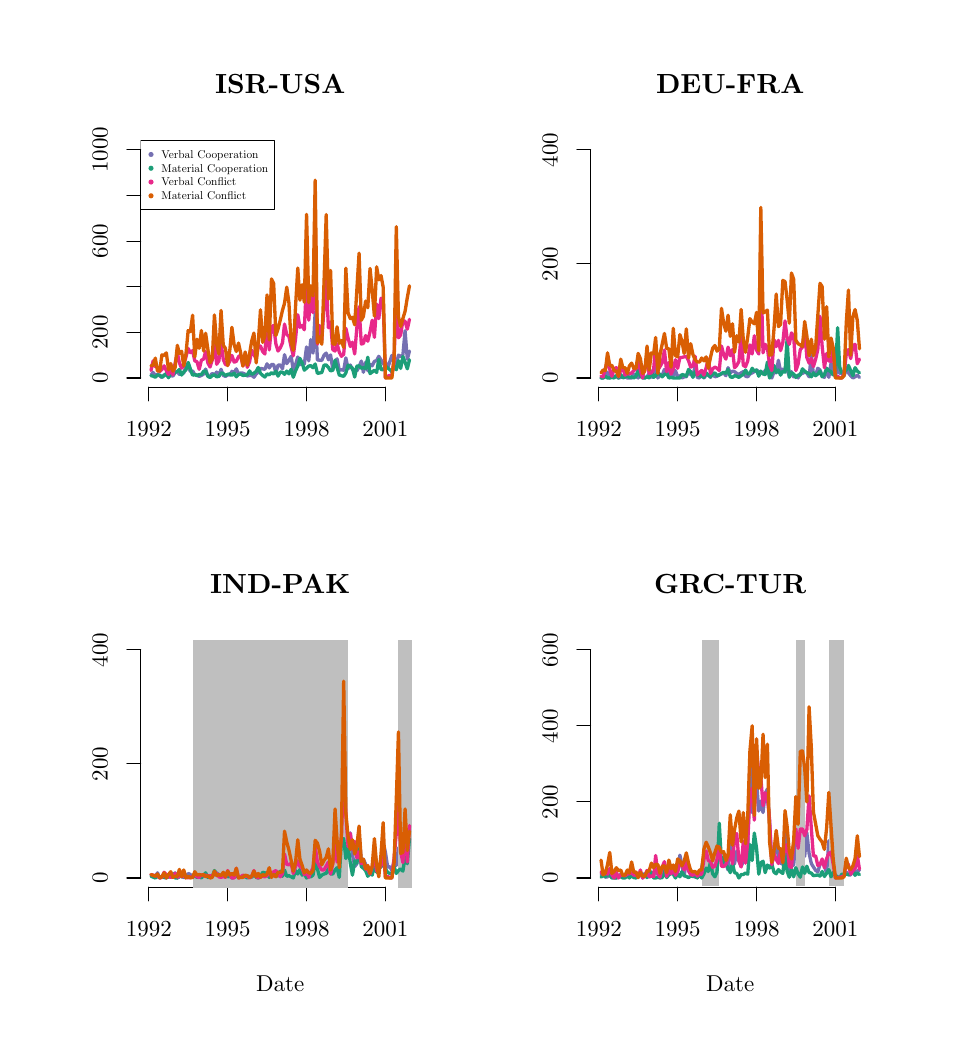
\begin{tikzpicture}[x=1pt,y=1pt]
\definecolor[named]{fillColor}{rgb}{1.00,1.00,1.00}
\path[use as bounding box,fill=fillColor,fill opacity=0.00] (0,0) rectangle (325.21,361.35);
\begin{scope}
\path[clip] ( 40.84,231.47) rectangle (141.69,320.51);
\definecolor[named]{drawColor}{rgb}{0.46,0.44,0.70}

\path[draw=drawColor,line width= 1.2pt,line join=round,line cap=round] ( 44.57,235.84) --
	( 45.33,236.75) --
	( 46.13,235.68) --
	( 46.91,236.09) --
	( 47.72,235.51) --
	( 48.50,234.93) --
	( 49.30,235.92) --
	( 50.11,235.84) --
	( 50.89,235.18) --
	( 51.70,235.68) --
	( 52.48,235.43) --
	( 53.28,236.67) --
	( 54.09,237.08) --
	( 54.82,236.01) --
	( 55.62,236.34) --
	( 56.40,236.58) --
	( 57.21,238.89) --
	( 57.99,239.06) --
	( 58.80,237.08) --
	( 59.60,237.32) --
	( 60.38,236.01) --
	( 61.19,235.84) --
	( 61.97,235.35) --
	( 62.78,235.68) --
	( 63.58,236.17) --
	( 64.31,237.98) --
	( 65.12,235.35) --
	( 65.90,235.51) --
	( 66.70,236.42) --
	( 67.48,235.76) --
	( 68.29,236.91) --
	( 69.09,235.35) --
	( 69.87,237.90) --
	( 70.68,235.68) --
	( 71.46,235.35) --
	( 72.27,235.84) --
	( 73.07,235.84) --
	( 73.80,237.16) --
	( 74.61,236.67) --
	( 75.39,238.07) --
	( 76.19,236.17) --
	( 76.97,236.58) --
	( 77.78,236.50) --
	( 78.59,236.09) --
	( 79.37,235.51) --
	( 80.17,235.68) --
	( 80.95,235.76) --
	( 81.76,235.02) --
	( 82.57,236.25) --
	( 83.32,236.83) --
	( 84.13,238.23) --
	( 84.91,238.07) --
	( 85.71,237.90) --
	( 86.49,239.88) --
	( 87.30,238.40) --
	( 88.10,239.63) --
	( 88.88,239.63) --
	( 89.69,236.67) --
	( 90.47,239.39) --
	( 91.28,239.47) --
	( 92.08,238.07) --
	( 92.81,243.18) --
	( 93.62,239.96) --
	( 94.40,241.12) --
	( 95.20,242.60) --
	( 95.98,237.57) --
	( 96.79,239.55) --
	( 97.60,242.35) --
	( 98.38,239.55) --
	( 99.18,240.05) --
	( 99.96,239.80) --
	(100.77,245.98) --
	(101.57,240.95) --
	(102.30,248.62) --
	(103.11,243.76) --
	(103.89,258.76) --
	(104.70,241.28) --
	(105.48,241.20) --
	(106.28,241.12) --
	(107.09,243.01) --
	(107.87,243.76) --
	(108.67,241.36) --
	(109.45,243.10) --
	(110.26,237.90) --
	(111.07,240.46) --
	(111.79,241.69) --
	(112.60,237.57) --
	(113.38,237.74) --
	(114.19,237.57) --
	(114.97,242.02) --
	(115.77,238.07) --
	(116.58,239.47) --
	(117.36,237.74) --
	(118.17,237.65) --
	(118.95,237.32) --
	(119.75,238.81) --
	(120.56,240.87) --
	(121.31,236.83) --
	(122.12,240.46) --
	(122.90,237.41) --
	(123.71,239.72) --
	(124.49,239.14) --
	(125.29,240.79) --
	(126.10,241.03) --
	(126.88,242.60) --
	(127.68,241.28) --
	(128.46,239.80) --
	(129.27,240.46) --
	(130.08,238.48) --
	(130.80,240.46) --
	(131.61,242.93) --
	(132.39,240.29) --
	(133.20,239.47) --
	(133.98,243.01) --
	(134.78,242.52) --
	(135.59,243.10) --
	(136.37,251.84) --
	(137.18,241.53) --
	(137.96,244.50);
\end{scope}
\begin{scope}
\path[clip] (  0.00,180.67) rectangle (162.61,361.35);
\definecolor[named]{drawColor}{rgb}{0.00,0.00,0.00}

\node[text=drawColor,anchor=base,inner sep=0pt, outer sep=0pt, scale=  1.00] at ( 91.26,337.50) {\bfseries ISR-USA};
\end{scope}
\begin{scope}
\path[clip] (  0.00,  0.00) rectangle (325.21,361.35);
\definecolor[named]{drawColor}{rgb}{0.00,0.00,0.00}

\path[draw=drawColor,line width= 0.4pt,line join=round,line cap=round] ( 43.77,231.47) -- (129.27,231.47);

\path[draw=drawColor,line width= 0.4pt,line join=round,line cap=round] ( 43.77,231.47) -- ( 43.77,226.49);

\path[draw=drawColor,line width= 0.4pt,line join=round,line cap=round] ( 72.27,231.47) -- ( 72.27,226.49);

\path[draw=drawColor,line width= 0.4pt,line join=round,line cap=round] (100.77,231.47) -- (100.77,226.49);

\path[draw=drawColor,line width= 0.4pt,line join=round,line cap=round] (129.27,231.47) -- (129.27,226.49);

\node[text=drawColor,anchor=base,inner sep=0pt, outer sep=0pt, scale=  0.83] at ( 43.77,213.54) {1992};

\node[text=drawColor,anchor=base,inner sep=0pt, outer sep=0pt, scale=  0.83] at ( 72.27,213.54) {1995};

\node[text=drawColor,anchor=base,inner sep=0pt, outer sep=0pt, scale=  0.83] at (100.77,213.54) {1998};

\node[text=drawColor,anchor=base,inner sep=0pt, outer sep=0pt, scale=  0.83] at (129.27,213.54) {2001};

\path[draw=drawColor,line width= 0.4pt,line join=round,line cap=round] ( 40.84,234.77) -- ( 40.84,317.22);

\path[draw=drawColor,line width= 0.4pt,line join=round,line cap=round] ( 40.84,234.77) -- ( 35.86,234.77);

\path[draw=drawColor,line width= 0.4pt,line join=round,line cap=round] ( 40.84,251.26) -- ( 35.86,251.26);

\path[draw=drawColor,line width= 0.4pt,line join=round,line cap=round] ( 40.84,267.75) -- ( 35.86,267.75);

\path[draw=drawColor,line width= 0.4pt,line join=round,line cap=round] ( 40.84,284.24) -- ( 35.86,284.24);

\path[draw=drawColor,line width= 0.4pt,line join=round,line cap=round] ( 40.84,300.73) -- ( 35.86,300.73);

\path[draw=drawColor,line width= 0.4pt,line join=round,line cap=round] ( 40.84,317.22) -- ( 35.86,317.22);

\node[text=drawColor,rotate= 90.00,anchor=base,inner sep=0pt, outer sep=0pt, scale=  0.83] at ( 28.88,234.77) {0};

\node[text=drawColor,rotate= 90.00,anchor=base,inner sep=0pt, outer sep=0pt, scale=  0.83] at ( 28.88,251.26) {200};

\node[text=drawColor,rotate= 90.00,anchor=base,inner sep=0pt, outer sep=0pt, scale=  0.83] at ( 28.88,284.24) {600};

\node[text=drawColor,rotate= 90.00,anchor=base,inner sep=0pt, outer sep=0pt, scale=  0.83] at ( 28.88,317.22) {1000};
\end{scope}
\begin{scope}
\path[clip] ( 40.84,231.47) rectangle (141.69,320.51);
\definecolor[named]{drawColor}{rgb}{0.11,0.62,0.47}

\path[draw=drawColor,line width= 1.2pt,line join=round,line cap=round] ( 44.57,235.59) --
	( 45.33,235.43) --
	( 46.13,235.02) --
	( 46.91,235.84) --
	( 47.72,235.84) --
	( 48.50,235.02) --
	( 49.30,235.59) --
	( 50.11,236.42) --
	( 50.89,234.85) --
	( 51.70,236.58) --
	( 52.48,236.09) --
	( 53.28,236.83) --
	( 54.09,237.16) --
	( 54.82,237.82) --
	( 55.62,235.84) --
	( 56.40,236.99) --
	( 57.21,237.74) --
	( 57.99,240.38) --
	( 58.80,237.98) --
	( 59.60,235.76) --
	( 60.38,236.01) --
	( 61.19,235.59) --
	( 61.97,236.01) --
	( 62.78,236.01) --
	( 63.58,237.16) --
	( 64.31,237.32) --
	( 65.12,235.35) --
	( 65.90,234.93) --
	( 66.70,235.59) --
	( 67.48,235.92) --
	( 68.29,235.18) --
	( 69.09,235.35) --
	( 69.87,236.58) --
	( 70.68,236.34) --
	( 71.46,235.68) --
	( 72.27,236.09) --
	( 73.07,236.25) --
	( 73.80,235.68) --
	( 74.61,236.50) --
	( 75.39,235.18) --
	( 76.19,236.01) --
	( 76.97,236.17) --
	( 77.78,235.68) --
	( 78.59,235.76) --
	( 79.37,235.92) --
	( 80.17,237.32) --
	( 80.95,236.09) --
	( 81.76,236.50) --
	( 82.57,237.16) --
	( 83.32,238.56) --
	( 84.13,236.42) --
	( 84.91,235.68) --
	( 85.71,235.10) --
	( 86.49,236.25) --
	( 87.30,235.92) --
	( 88.10,236.67) --
	( 88.88,236.17) --
	( 89.69,237.24) --
	( 90.47,235.43) --
	( 91.28,236.91) --
	( 92.08,236.83) --
	( 92.81,236.09) --
	( 93.62,237.24) --
	( 94.40,236.25) --
	( 95.20,237.90) --
	( 95.98,235.02) --
	( 96.79,237.32) --
	( 97.60,239.06) --
	( 98.38,241.86) --
	( 99.18,240.21) --
	( 99.96,237.57) --
	(100.77,238.31) --
	(101.57,239.06) --
	(102.30,239.22) --
	(103.11,238.48) --
	(103.89,239.80) --
	(104.70,236.42) --
	(105.48,236.58) --
	(106.28,236.75) --
	(107.09,239.39) --
	(107.87,239.47) --
	(108.67,238.56) --
	(109.45,237.32) --
	(110.26,237.57) --
	(111.07,241.20) --
	(111.79,238.56) --
	(112.60,235.84) --
	(113.38,235.59) --
	(114.19,235.35) --
	(114.97,236.58) --
	(115.77,239.39) --
	(116.58,238.89) --
	(117.36,238.31) --
	(118.17,235.10) --
	(118.95,239.06) --
	(119.75,239.14) --
	(120.56,238.31) --
	(121.31,238.48) --
	(122.12,238.15) --
	(122.90,242.27) --
	(123.71,236.34) --
	(124.49,236.91) --
	(125.29,237.57) --
	(126.10,236.75) --
	(126.88,241.45) --
	(127.68,237.82) --
	(128.46,237.74) --
	(129.27,239.06) --
	(130.08,238.40) --
	(130.80,237.82) --
	(131.61,236.99) --
	(132.39,238.97) --
	(133.20,237.74) --
	(133.98,241.03) --
	(134.78,238.23) --
	(135.59,242.52) --
	(136.37,240.46) --
	(137.18,238.07) --
	(137.96,241.36);
\definecolor[named]{drawColor}{rgb}{0.91,0.16,0.54}

\path[draw=drawColor,line width= 1.2pt,line join=round,line cap=round] ( 44.57,237.49) --
	( 45.33,240.95) --
	( 46.13,238.89) --
	( 46.91,238.73) --
	( 47.72,237.08) --
	( 48.50,237.82) --
	( 49.30,239.14) --
	( 50.11,237.41) --
	( 50.89,236.01) --
	( 51.70,238.15) --
	( 52.48,235.92) --
	( 53.28,240.13) --
	( 54.09,243.84) --
	( 54.82,240.21) --
	( 55.62,238.31) --
	( 56.40,239.30) --
	( 57.21,242.44) --
	( 57.99,245.40) --
	( 58.80,243.92) --
	( 59.60,244.66) --
	( 60.38,240.95) --
	( 61.19,240.62) --
	( 61.97,237.90) --
	( 62.78,241.20) --
	( 63.58,241.61) --
	( 64.31,244.33) --
	( 65.12,240.21) --
	( 65.90,238.73) --
	( 66.70,241.28) --
	( 67.48,248.13) --
	( 68.29,239.72) --
	( 69.09,240.95) --
	( 69.87,247.71) --
	( 70.68,241.45) --
	( 71.46,239.63) --
	( 72.27,239.39) --
	( 73.07,240.87) --
	( 73.80,242.93) --
	( 74.61,240.46) --
	( 75.39,240.79) --
	( 76.19,242.44) --
	( 76.97,243.10) --
	( 77.78,239.14) --
	( 78.59,242.27) --
	( 79.37,238.64) --
	( 80.17,240.54) --
	( 80.95,244.83) --
	( 81.76,243.26) --
	( 82.57,241.53) --
	( 83.32,246.39) --
	( 84.13,246.31) --
	( 84.91,244.33) --
	( 85.71,243.43) --
	( 86.49,254.80) --
	( 87.30,244.91) --
	( 88.10,253.24) --
	( 88.88,253.73) --
	( 89.69,247.05) --
	( 90.47,244.50) --
	( 91.28,245.65) --
	( 92.08,247.47) --
	( 92.81,254.23) --
	( 93.62,250.43) --
	( 94.40,249.86) --
	( 95.20,245.90) --
	( 95.98,242.77) --
	( 96.79,248.87) --
	( 97.60,257.61) --
	( 98.38,253.07) --
	( 99.18,253.73) --
	( 99.96,252.17) --
	(100.77,269.73) --
	(101.57,255.63) --
	(102.30,264.86) --
	(103.11,258.35) --
	(103.89,289.51) --
	(104.70,246.97) --
	(105.48,253.73) --
	(106.28,248.37) --
	(107.09,260.16) --
	(107.87,270.22) --
	(108.67,252.91) --
	(109.45,254.97) --
	(110.26,244.99) --
	(111.07,244.50) --
	(111.79,247.14) --
	(112.60,244.09) --
	(113.38,242.60) --
	(114.19,243.34) --
	(114.97,252.74) --
	(115.77,249.20) --
	(116.58,246.15) --
	(117.36,247.71) --
	(118.17,243.43) --
	(118.95,253.07) --
	(119.75,260.49) --
	(120.56,247.05) --
	(121.31,247.22) --
	(122.12,250.10) --
	(122.90,248.04) --
	(123.71,251.42) --
	(124.49,255.63) --
	(125.29,249.44) --
	(126.10,261.48) --
	(126.88,256.21) --
	(127.68,263.54) --
	(128.46,263.38) --
	(129.27,234.77) --
	(130.08,235.43) --
	(130.80,235.68) --
	(131.61,235.59) --
	(132.39,241.20) --
	(133.20,264.12) --
	(133.98,249.28) --
	(134.78,250.35) --
	(135.59,255.55) --
	(136.37,255.22) --
	(137.18,252.41) --
	(137.96,255.96);
\definecolor[named]{drawColor}{rgb}{0.85,0.37,0.01}

\path[draw=drawColor,line width= 1.2pt,line join=round,line cap=round] ( 44.57,239.22) --
	( 45.33,239.39) --
	( 46.13,241.94) --
	( 46.91,237.24) --
	( 47.72,237.32) --
	( 48.50,243.10) --
	( 49.30,242.93) --
	( 50.11,243.84) --
	( 50.89,237.74) --
	( 51.70,239.96) --
	( 52.48,237.24) --
	( 53.28,238.56) --
	( 54.09,246.56) --
	( 54.82,243.59) --
	( 55.62,244.42) --
	( 56.40,239.14) --
	( 57.21,243.59) --
	( 57.99,251.92) --
	( 58.80,251.51) --
	( 59.60,257.44) --
	( 60.38,242.35) --
	( 61.19,248.78) --
	( 61.97,245.49) --
	( 62.78,251.92) --
	( 63.58,244.50) --
	( 64.31,250.93) --
	( 65.12,245.07) --
	( 65.90,240.29) --
	( 66.70,241.61) --
	( 67.48,257.52) --
	( 68.29,246.97) --
	( 69.09,243.43) --
	( 69.87,259.17) --
	( 70.68,246.56) --
	( 71.46,245.49) --
	( 72.27,239.22) --
	( 73.07,245.07) --
	( 73.80,253.07) --
	( 74.61,246.72) --
	( 75.39,244.33) --
	( 76.19,247.38) --
	( 76.97,243.76) --
	( 77.78,239.06) --
	( 78.59,244.17) --
	( 79.37,239.30) --
	( 80.17,243.43) --
	( 80.95,248.13) --
	( 81.76,251.01) --
	( 82.57,240.21) --
	( 83.32,247.63) --
	( 84.13,259.42) --
	( 84.91,247.63) --
	( 85.71,249.94) --
	( 86.49,264.78) --
	( 87.30,248.54) --
	( 88.10,270.55) --
	( 88.88,268.90) --
	( 89.69,250.10) --
	( 90.47,252.50) --
	( 91.28,255.71) --
	( 92.08,259.26) --
	( 92.81,261.73) --
	( 93.62,267.58) --
	( 94.40,261.89) --
	( 95.20,247.80) --
	( 95.98,244.75) --
	( 96.79,260.49) --
	( 97.60,274.51) --
	( 98.38,262.88) --
	( 99.18,268.49) --
	( 99.96,262.14) --
	(100.77,293.88) --
	(101.57,261.98) --
	(102.30,268.08) --
	(103.11,264.45) --
	(103.89,306.25) --
	(104.70,247.38) --
	(105.48,249.61) --
	(106.28,246.97) --
	(107.09,269.48) --
	(107.87,293.80) --
	(108.67,263.30) --
	(109.45,273.60) --
	(110.26,247.14) --
	(111.07,246.97) --
	(111.79,253.24) --
	(112.60,247.30) --
	(113.38,248.29) --
	(114.19,245.82) --
	(114.97,274.43) --
	(115.77,258.35) --
	(116.58,256.21) --
	(117.36,256.70) --
	(118.17,253.98) --
	(118.95,266.68) --
	(119.75,279.87) --
	(120.56,255.63) --
	(121.31,257.03) --
	(122.12,262.55) --
	(122.90,260.16) --
	(123.71,274.34) --
	(124.49,266.51) --
	(125.29,257.11) --
	(126.10,274.92) --
	(126.88,270.22) --
	(127.68,271.79) --
	(128.46,267.58) --
	(129.27,234.77) --
	(130.08,234.77) --
	(130.80,234.77) --
	(131.61,234.77) --
	(132.39,242.02) --
	(133.20,289.43) --
	(133.98,256.86) --
	(134.78,253.40) --
	(135.59,256.29) --
	(136.37,258.84) --
	(137.18,263.79) --
	(137.96,268.08);
\definecolor[named]{drawColor}{rgb}{0.00,0.00,0.00}

\path[draw=drawColor,line width= 0.4pt,line join=round,line cap=round] ( 40.84,320.51) rectangle ( 89.27,295.61);
\definecolor[named]{fillColor}{rgb}{0.46,0.44,0.70}

\path[fill=fillColor] ( 44.57,315.53) circle (  0.93);
\definecolor[named]{fillColor}{rgb}{0.11,0.62,0.47}

\path[fill=fillColor] ( 44.57,310.55) circle (  0.93);
\definecolor[named]{fillColor}{rgb}{0.91,0.16,0.54}

\path[fill=fillColor] ( 44.57,305.57) circle (  0.93);
\definecolor[named]{fillColor}{rgb}{0.85,0.37,0.01}

\path[fill=fillColor] ( 44.57,300.59) circle (  0.93);

\node[text=drawColor,anchor=base west,inner sep=0pt, outer sep=0pt, scale=  0.41] at ( 48.31,314.10) {Verbal Cooperation};

\node[text=drawColor,anchor=base west,inner sep=0pt, outer sep=0pt, scale=  0.41] at ( 48.31,309.12) {Material Cooperation};

\node[text=drawColor,anchor=base west,inner sep=0pt, outer sep=0pt, scale=  0.41] at ( 48.31,304.14) {Verbal Conflict};

\node[text=drawColor,anchor=base west,inner sep=0pt, outer sep=0pt, scale=  0.41] at ( 48.31,299.16) {Material Conflict};
\end{scope}
\begin{scope}
\path[clip] (203.44,231.47) rectangle (304.30,320.51);
\definecolor[named]{drawColor}{rgb}{0.46,0.44,0.70}

\path[draw=drawColor,line width= 1.2pt,line join=round,line cap=round] (207.18,234.77) --
	(207.93,234.77) --
	(208.74,235.18) --
	(209.52,236.83) --
	(210.33,234.77) --
	(211.11,235.59) --
	(211.91,235.39) --
	(212.72,235.39) --
	(213.50,234.77) --
	(214.30,234.98) --
	(215.08,235.39) --
	(215.89,235.18) --
	(216.70,234.77) --
	(217.42,234.77) --
	(218.23,234.77) --
	(219.01,236.21) --
	(219.82,235.39) --
	(220.60,234.77) --
	(221.40,236.21) --
	(222.21,235.18) --
	(222.99,234.77) --
	(223.80,235.18) --
	(224.58,236.42) --
	(225.38,234.98) --
	(226.19,235.39) --
	(226.92,238.27) --
	(227.72,234.77) --
	(228.50,235.80) --
	(229.31,235.80) --
	(230.09,237.86) --
	(230.90,237.24) --
	(231.70,235.39) --
	(232.48,236.83) --
	(233.29,235.59) --
	(234.07,237.45) --
	(234.87,235.18) --
	(235.68,235.59) --
	(236.41,234.77) --
	(237.21,235.18) --
	(238.00,235.18) --
	(238.80,237.04) --
	(239.58,236.01) --
	(240.39,235.59) --
	(241.19,239.10) --
	(241.97,234.98) --
	(242.78,234.77) --
	(243.56,237.45) --
	(244.37,234.77) --
	(245.17,235.80) --
	(245.93,236.01) --
	(246.73,234.98) --
	(247.51,236.62) --
	(248.32,235.18) --
	(249.10,235.39) --
	(249.91,236.01) --
	(250.71,236.21) --
	(251.49,236.62) --
	(252.30,235.59) --
	(253.08,238.48) --
	(253.88,236.62) --
	(254.69,237.24) --
	(255.42,237.04) --
	(256.22,236.42) --
	(257.00,236.01) --
	(257.81,236.62) --
	(258.59,237.04) --
	(259.40,235.39) --
	(260.20,235.18) --
	(260.98,236.21) --
	(261.79,236.62) --
	(262.57,237.04) --
	(263.38,237.65) --
	(264.18,237.04) --
	(264.91,236.83) --
	(265.72,236.42) --
	(266.50,237.45) --
	(267.30,238.07) --
	(268.08,235.18) --
	(268.89,234.77) --
	(269.70,237.04) --
	(270.48,236.62) --
	(271.28,241.16) --
	(272.06,237.04) --
	(272.87,238.07) --
	(273.67,237.45) --
	(274.40,237.86) --
	(275.21,235.39) --
	(275.99,237.04) --
	(276.79,235.18) --
	(277.58,235.59) --
	(278.38,234.77) --
	(279.19,236.42) --
	(279.97,236.42) --
	(280.77,236.83) --
	(281.55,236.62) --
	(282.36,235.18) --
	(283.17,243.01) --
	(283.92,236.01) --
	(284.73,235.80) --
	(285.51,238.27) --
	(286.31,237.65) --
	(287.09,235.59) --
	(287.90,234.98) --
	(288.71,238.27) --
	(289.49,234.98) --
	(290.29,240.13) --
	(291.07,238.27) --
	(291.88,235.18) --
	(292.68,240.33) --
	(293.41,236.42) --
	(294.22,236.42) --
	(295.00,235.59) --
	(295.80,238.07) --
	(296.58,236.62) --
	(297.39,235.59) --
	(298.20,234.77) --
	(298.98,235.18) --
	(299.78,235.80) --
	(300.56,234.98);
\end{scope}
\begin{scope}
\path[clip] (162.61,180.67) rectangle (325.21,361.35);
\definecolor[named]{drawColor}{rgb}{0.00,0.00,0.00}

\node[text=drawColor,anchor=base,inner sep=0pt, outer sep=0pt, scale=  1.00] at (253.87,337.50) {\bfseries DEU-FRA};
\end{scope}
\begin{scope}
\path[clip] (  0.00,  0.00) rectangle (325.21,361.35);
\definecolor[named]{drawColor}{rgb}{0.00,0.00,0.00}

\path[draw=drawColor,line width= 0.4pt,line join=round,line cap=round] (206.37,231.47) -- (291.88,231.47);

\path[draw=drawColor,line width= 0.4pt,line join=round,line cap=round] (206.37,231.47) -- (206.37,226.49);

\path[draw=drawColor,line width= 0.4pt,line join=round,line cap=round] (234.87,231.47) -- (234.87,226.49);

\path[draw=drawColor,line width= 0.4pt,line join=round,line cap=round] (263.38,231.47) -- (263.38,226.49);

\path[draw=drawColor,line width= 0.4pt,line join=round,line cap=round] (291.88,231.47) -- (291.88,226.49);

\node[text=drawColor,anchor=base,inner sep=0pt, outer sep=0pt, scale=  0.83] at (206.37,213.54) {1992};

\node[text=drawColor,anchor=base,inner sep=0pt, outer sep=0pt, scale=  0.83] at (234.87,213.54) {1995};

\node[text=drawColor,anchor=base,inner sep=0pt, outer sep=0pt, scale=  0.83] at (263.38,213.54) {1998};

\node[text=drawColor,anchor=base,inner sep=0pt, outer sep=0pt, scale=  0.83] at (291.88,213.54) {2001};

\path[draw=drawColor,line width= 0.4pt,line join=round,line cap=round] (203.44,234.77) -- (203.44,317.22);

\path[draw=drawColor,line width= 0.4pt,line join=round,line cap=round] (203.44,234.77) -- (198.46,234.77);

\path[draw=drawColor,line width= 0.4pt,line join=round,line cap=round] (203.44,275.99) -- (198.46,275.99);

\path[draw=drawColor,line width= 0.4pt,line join=round,line cap=round] (203.44,317.22) -- (198.46,317.22);

\node[text=drawColor,rotate= 90.00,anchor=base,inner sep=0pt, outer sep=0pt, scale=  0.83] at (191.49,234.77) {0};

\node[text=drawColor,rotate= 90.00,anchor=base,inner sep=0pt, outer sep=0pt, scale=  0.83] at (191.49,275.99) {200};

\node[text=drawColor,rotate= 90.00,anchor=base,inner sep=0pt, outer sep=0pt, scale=  0.83] at (191.49,317.22) {400};
\end{scope}
\begin{scope}
\path[clip] (203.44,231.47) rectangle (304.30,320.51);
\definecolor[named]{drawColor}{rgb}{0.11,0.62,0.47}

\path[draw=drawColor,line width= 1.2pt,line join=round,line cap=round] (207.18,234.77) --
	(207.93,234.77) --
	(208.74,235.39) --
	(209.52,234.77) --
	(210.33,234.77) --
	(211.11,234.98) --
	(211.91,234.77) --
	(212.72,235.59) --
	(213.50,234.77) --
	(214.30,236.01) --
	(215.08,234.77) --
	(215.89,235.18) --
	(216.70,235.59) --
	(217.42,234.98) --
	(218.23,235.18) --
	(219.01,234.77) --
	(219.82,235.39) --
	(220.60,237.86) --
	(221.40,235.39) --
	(222.21,234.77) --
	(222.99,234.77) --
	(223.80,235.18) --
	(224.58,234.77) --
	(225.38,237.24) --
	(226.19,234.98) --
	(226.92,235.59) --
	(227.72,236.62) --
	(228.50,236.01) --
	(229.31,235.18) --
	(230.09,236.01) --
	(230.90,236.42) --
	(231.70,234.77) --
	(232.48,234.98) --
	(233.29,234.77) --
	(234.07,234.77) --
	(234.87,234.77) --
	(235.68,234.77) --
	(236.41,236.01) --
	(237.21,235.80) --
	(238.00,235.39) --
	(238.80,237.86) --
	(239.58,237.04) --
	(240.39,234.98) --
	(241.19,237.04) --
	(241.97,235.80) --
	(242.78,235.59) --
	(243.56,235.39) --
	(244.37,234.98) --
	(245.17,236.62) --
	(245.93,235.80) --
	(246.73,235.18) --
	(247.51,236.21) --
	(248.32,236.62) --
	(249.10,235.59) --
	(249.91,235.80) --
	(250.71,236.42) --
	(251.49,236.83) --
	(252.30,236.42) --
	(253.08,237.86) --
	(253.88,235.18) --
	(254.69,234.98) --
	(255.42,235.59) --
	(256.22,235.39) --
	(257.00,234.98) --
	(257.81,235.59) --
	(258.59,236.01) --
	(259.40,237.65) --
	(260.20,236.21) --
	(260.98,236.42) --
	(261.79,238.27) --
	(262.57,237.24) --
	(263.38,237.65) --
	(264.18,235.39) --
	(264.91,237.24) --
	(265.72,236.21) --
	(266.50,236.01) --
	(267.30,240.54) --
	(268.08,234.77) --
	(268.89,236.21) --
	(269.70,239.30) --
	(270.48,236.83) --
	(271.28,237.65) --
	(272.06,235.80) --
	(272.87,237.24) --
	(273.67,236.83) --
	(274.40,248.78) --
	(275.21,234.98) --
	(275.99,236.62) --
	(276.79,236.21) --
	(277.58,234.98) --
	(278.38,235.80) --
	(279.19,235.80) --
	(279.97,238.07) --
	(280.77,237.24) --
	(281.55,236.62) --
	(282.36,236.42) --
	(283.17,235.18) --
	(283.92,236.62) --
	(284.73,235.59) --
	(285.51,236.21) --
	(286.31,237.24) --
	(287.09,235.18) --
	(287.90,236.01) --
	(288.71,238.27) --
	(289.49,237.45) --
	(290.29,237.04) --
	(291.07,235.80) --
	(291.88,236.21) --
	(292.68,252.91) --
	(293.41,238.69) --
	(294.22,236.62) --
	(295.00,237.04) --
	(295.80,237.65) --
	(296.58,239.30) --
	(297.39,237.45) --
	(298.20,235.59) --
	(298.98,238.48) --
	(299.78,237.24) --
	(300.56,236.62);
\definecolor[named]{drawColor}{rgb}{0.91,0.16,0.54}

\path[draw=drawColor,line width= 1.2pt,line join=round,line cap=round] (207.18,235.39) --
	(207.93,235.18) --
	(208.74,238.27) --
	(209.52,240.95) --
	(210.33,237.86) --
	(211.11,235.39) --
	(211.91,238.07) --
	(212.72,238.48) --
	(213.50,235.18) --
	(214.30,237.65) --
	(215.08,238.07) --
	(215.89,235.80) --
	(216.70,236.42) --
	(217.42,236.21) --
	(218.23,236.62) --
	(219.01,237.45) --
	(219.82,238.07) --
	(220.60,240.54) --
	(221.40,237.45) --
	(222.21,234.77) --
	(222.99,238.89) --
	(223.80,239.92) --
	(224.58,236.42) --
	(225.38,236.62) --
	(226.19,237.86) --
	(226.92,246.52) --
	(227.72,237.65) --
	(228.50,238.89) --
	(229.31,240.33) --
	(230.09,244.87) --
	(230.90,237.04) --
	(231.70,240.33) --
	(232.48,236.21) --
	(233.29,237.86) --
	(234.07,241.36) --
	(234.87,238.27) --
	(235.68,242.19) --
	(236.41,242.19) --
	(237.21,242.40) --
	(238.00,242.60) --
	(238.80,240.95) --
	(239.58,238.69) --
	(240.39,239.10) --
	(241.19,242.60) --
	(241.97,235.80) --
	(242.78,236.83) --
	(243.56,237.45) --
	(244.37,235.80) --
	(245.17,238.48) --
	(245.93,241.57) --
	(246.73,236.42) --
	(247.51,238.07) --
	(248.32,238.69) --
	(249.10,238.27) --
	(249.91,237.45) --
	(250.71,246.31) --
	(251.49,243.22) --
	(252.30,241.57) --
	(253.08,245.90) --
	(253.88,242.81) --
	(254.69,245.07) --
	(255.42,238.48) --
	(256.22,239.30) --
	(257.00,240.75) --
	(257.81,250.43) --
	(258.59,239.30) --
	(259.40,238.89) --
	(260.20,240.95) --
	(260.98,246.72) --
	(261.79,243.43) --
	(262.57,250.02) --
	(263.38,244.87) --
	(264.18,243.43) --
	(264.91,274.96) --
	(265.72,243.84) --
	(266.50,246.93) --
	(267.30,245.69) --
	(268.08,239.51) --
	(268.89,237.45) --
	(269.70,248.58) --
	(270.48,246.11) --
	(271.28,248.37) --
	(272.06,244.66) --
	(272.87,247.55) --
	(273.67,255.38) --
	(274.40,249.20) --
	(275.21,246.93) --
	(275.99,251.05) --
	(276.79,249.82) --
	(277.58,237.45) --
	(278.38,239.72) --
	(279.19,245.07) --
	(279.97,245.90) --
	(280.77,252.29) --
	(281.55,242.19) --
	(282.36,240.13) --
	(283.17,241.78) --
	(283.92,238.89) --
	(284.73,241.57) --
	(285.51,245.07) --
	(286.31,257.03) --
	(287.09,246.11) --
	(287.90,238.48) --
	(288.71,243.63) --
	(289.49,240.95) --
	(290.29,240.75) --
	(291.07,245.28) --
	(291.88,235.18) --
	(292.68,235.39) --
	(293.41,234.77) --
	(294.22,234.77) --
	(295.00,236.21) --
	(295.80,243.43) --
	(296.58,245.07) --
	(297.39,241.78) --
	(298.20,246.31) --
	(298.98,246.93) --
	(299.78,239.92) --
	(300.56,241.57);
\definecolor[named]{drawColor}{rgb}{0.85,0.37,0.01}

\path[draw=drawColor,line width= 1.2pt,line join=round,line cap=round] (207.18,236.62) --
	(207.93,237.65) --
	(208.74,237.45) --
	(209.52,243.84) --
	(210.33,239.30) --
	(211.11,239.30) --
	(211.91,237.45) --
	(212.72,237.24) --
	(213.50,235.39) --
	(214.30,241.57) --
	(215.08,238.48) --
	(215.89,238.48) --
	(216.70,236.42) --
	(217.42,239.10) --
	(218.23,240.13) --
	(219.01,238.27) --
	(219.82,238.27) --
	(220.60,243.63) --
	(221.40,241.78) --
	(222.21,236.42) --
	(222.99,237.24) --
	(223.80,246.31) --
	(224.58,237.65) --
	(225.38,243.84) --
	(226.19,243.43) --
	(226.92,249.40) --
	(227.72,236.42) --
	(228.50,243.22) --
	(229.31,247.14) --
	(230.09,250.85) --
	(230.90,245.49) --
	(231.70,245.28) --
	(232.48,238.69) --
	(233.29,252.70) --
	(234.07,242.81) --
	(234.87,242.40) --
	(235.68,250.43) --
	(236.41,248.17) --
	(237.21,243.63) --
	(238.00,252.50) --
	(238.80,241.98) --
	(239.58,247.14) --
	(240.39,243.22) --
	(241.19,241.36) --
	(241.97,240.54) --
	(242.78,240.54) --
	(243.56,241.98) --
	(244.37,240.95) --
	(245.17,242.40) --
	(245.93,238.27) --
	(246.73,242.19) --
	(247.51,245.49) --
	(248.32,246.52) --
	(249.10,244.46) --
	(249.91,245.28) --
	(250.71,259.92) --
	(251.49,254.56) --
	(252.30,251.67) --
	(253.08,257.44) --
	(253.88,249.82) --
	(254.69,254.35) --
	(255.42,244.04) --
	(256.22,250.02) --
	(257.00,247.75) --
	(257.81,259.50) --
	(258.59,248.58) --
	(259.40,244.04) --
	(260.20,249.61) --
	(260.98,256.21) --
	(261.79,254.97) --
	(262.57,254.35) --
	(263.38,258.47) --
	(264.18,244.66) --
	(264.91,296.40) --
	(265.72,258.27) --
	(266.50,258.68) --
	(267.30,259.30) --
	(268.08,243.01) --
	(268.89,243.22) --
	(269.70,252.70) --
	(270.48,265.07) --
	(271.28,253.32) --
	(272.06,254.14) --
	(272.87,270.02) --
	(273.67,269.60) --
	(274.40,263.21) --
	(275.21,254.56) --
	(275.99,272.69) --
	(276.79,270.43) --
	(277.58,248.37) --
	(278.38,247.14) --
	(279.19,246.72) --
	(279.97,246.11) --
	(280.77,255.17) --
	(281.55,250.02) --
	(282.36,242.81) --
	(283.17,248.78) --
	(283.92,242.81) --
	(284.73,245.90) --
	(285.51,257.24) --
	(286.31,268.98) --
	(287.09,267.75) --
	(287.90,248.78) --
	(288.71,260.53) --
	(289.49,242.40) --
	(290.29,249.20) --
	(291.07,245.69) --
	(291.88,234.77) --
	(292.68,234.77) --
	(293.41,234.77) --
	(294.22,234.77) --
	(295.00,235.59) --
	(295.80,254.76) --
	(296.58,266.51) --
	(297.39,243.01) --
	(298.20,257.03) --
	(298.98,259.50) --
	(299.78,255.59) --
	(300.56,245.28);
\end{scope}
\begin{scope}
\path[clip] ( 40.84, 50.80) rectangle (141.69,139.84);
\definecolor[named]{drawColor}{rgb}{0.46,0.44,0.70}

\path[draw=drawColor,line width= 1.2pt,line join=round,line cap=round] ( 44.57, 55.12) --
	( 46.13, 54.51) --
	( 46.91, 55.95) --
	( 47.72, 54.09) --
	( 48.50, 54.51) --
	( 49.30, 54.30) --
	( 50.11, 54.09) --
	( 50.89, 54.51) --
	( 51.70, 54.92) --
	( 52.48, 55.12) --
	( 53.28, 55.95) --
	( 54.09, 54.09) --
	( 54.82, 56.16) --
	( 55.62, 54.51) --
	( 56.40, 54.30) --
	( 57.21, 54.30) --
	( 57.99, 55.74) --
	( 58.80, 55.33) --
	( 59.60, 54.51) --
	( 60.38, 54.51) --
	( 61.19, 54.09) --
	( 61.97, 54.09) --
	( 62.78, 56.36) --
	( 63.58, 56.57) --
	( 64.31, 54.51) --
	( 65.12, 54.51) --
	( 65.90, 54.09) --
	( 66.70, 55.54) --
	( 67.48, 54.92) --
	( 68.29, 58.42) --
	( 69.09, 56.36) --
	( 69.87, 55.95) --
	( 70.68, 55.12) --
	( 71.46, 56.16) --
	( 72.27, 54.92) --
	( 73.07, 54.71) --
	( 73.80, 55.12) --
	( 74.61, 54.51) --
	( 75.39, 60.28) --
	( 76.19, 57.39) --
	( 76.97, 54.92) --
	( 77.78, 56.16) --
	( 78.59, 55.33) --
	( 79.37, 54.30) --
	( 80.17, 54.71) --
	( 80.95, 56.77) --
	( 81.76, 58.22) --
	( 82.57, 55.95) --
	( 83.32, 57.19) --
	( 84.13, 59.45) --
	( 84.91, 62.13) --
	( 85.71, 57.19) --
	( 86.49, 56.98) --
	( 87.30, 57.39) --
	( 88.10, 55.12) --
	( 88.88, 54.71) --
	( 89.69, 54.71) --
	( 90.47, 56.77) --
	( 91.28, 54.09) --
	( 92.08, 55.12) --
	( 92.81, 61.10) --
	( 93.62, 56.16) --
	( 94.40, 59.66) --
	( 95.20, 56.98) --
	( 95.98, 56.16) --
	( 96.79, 58.63) --
	( 97.60, 59.87) --
	( 98.38, 61.51) --
	( 99.18, 54.30) --
	( 99.96, 54.92) --
	(100.77, 55.54) --
	(101.57, 54.71) --
	(102.30, 56.77) --
	(103.11, 56.77) --
	(103.89, 61.72) --
	(104.70, 66.87) --
	(105.48, 57.39) --
	(106.28, 56.16) --
	(107.09, 59.45) --
	(107.87, 58.42) --
	(108.67, 56.57) --
	(109.45, 55.95) --
	(110.26, 56.16) --
	(111.07, 57.60) --
	(111.79, 58.01) --
	(112.60, 57.80) --
	(113.38, 72.85) --
	(114.19, 85.84) --
	(114.97, 69.35) --
	(115.77, 65.22) --
	(116.58, 70.38) --
	(117.36, 62.54) --
	(118.17, 58.22) --
	(118.95, 59.25) --
	(119.75, 69.55) --
	(120.56, 60.69) --
	(121.31, 60.90) --
	(122.12, 59.04) --
	(122.90, 55.95) --
	(123.71, 56.77) --
	(124.49, 56.98) --
	(125.29, 63.99) --
	(126.10, 58.83) --
	(126.88, 56.98) --
	(127.68, 60.07) --
	(128.46, 67.08) --
	(129.27, 63.37) --
	(130.08, 58.01) --
	(130.80, 58.22) --
	(131.61, 56.77) --
	(132.39, 60.28) --
	(133.20, 58.63) --
	(133.98, 65.02) --
	(134.78, 58.83) --
	(135.59, 64.19) --
	(136.37, 66.67) --
	(137.18, 63.16) --
	(137.96, 83.36);
\end{scope}
\begin{scope}
\path[clip] (  0.00,  0.00) rectangle (162.61,180.67);
\definecolor[named]{drawColor}{rgb}{0.00,0.00,0.00}

\node[text=drawColor,anchor=base,inner sep=0pt, outer sep=0pt, scale=  1.00] at ( 91.26,156.82) {\bfseries IND-PAK};

\node[text=drawColor,anchor=base,inner sep=0pt, outer sep=0pt, scale=  0.83] at ( 91.26, 12.95) {Date};
\end{scope}
\begin{scope}
\path[clip] (  0.00,  0.00) rectangle (325.21,361.35);
\definecolor[named]{drawColor}{rgb}{0.00,0.00,0.00}

\path[draw=drawColor,line width= 0.4pt,line join=round,line cap=round] ( 43.77, 50.80) -- (129.27, 50.80);

\path[draw=drawColor,line width= 0.4pt,line join=round,line cap=round] ( 43.77, 50.80) -- ( 43.77, 45.82);

\path[draw=drawColor,line width= 0.4pt,line join=round,line cap=round] ( 72.27, 50.80) -- ( 72.27, 45.82);

\path[draw=drawColor,line width= 0.4pt,line join=round,line cap=round] (100.77, 50.80) -- (100.77, 45.82);

\path[draw=drawColor,line width= 0.4pt,line join=round,line cap=round] (129.27, 50.80) -- (129.27, 45.82);

\node[text=drawColor,anchor=base,inner sep=0pt, outer sep=0pt, scale=  0.83] at ( 43.77, 32.87) {1992};

\node[text=drawColor,anchor=base,inner sep=0pt, outer sep=0pt, scale=  0.83] at ( 72.27, 32.87) {1995};

\node[text=drawColor,anchor=base,inner sep=0pt, outer sep=0pt, scale=  0.83] at (100.77, 32.87) {1998};

\node[text=drawColor,anchor=base,inner sep=0pt, outer sep=0pt, scale=  0.83] at (129.27, 32.87) {2001};

\path[draw=drawColor,line width= 0.4pt,line join=round,line cap=round] ( 40.84, 54.09) -- ( 40.84,136.54);

\path[draw=drawColor,line width= 0.4pt,line join=round,line cap=round] ( 40.84, 54.09) -- ( 35.86, 54.09);

\path[draw=drawColor,line width= 0.4pt,line join=round,line cap=round] ( 40.84, 95.32) -- ( 35.86, 95.32);

\path[draw=drawColor,line width= 0.4pt,line join=round,line cap=round] ( 40.84,136.54) -- ( 35.86,136.54);

\node[text=drawColor,rotate= 90.00,anchor=base,inner sep=0pt, outer sep=0pt, scale=  0.83] at ( 28.88, 54.09) {0};

\node[text=drawColor,rotate= 90.00,anchor=base,inner sep=0pt, outer sep=0pt, scale=  0.83] at ( 28.88, 95.32) {200};

\node[text=drawColor,rotate= 90.00,anchor=base,inner sep=0pt, outer sep=0pt, scale=  0.83] at ( 28.88,136.54) {400};
\end{scope}
\begin{scope}
\path[clip] ( 40.84, 50.80) rectangle (141.69,139.84);
\definecolor[named]{fillColor}{rgb}{0.75,0.75,0.75}

\path[fill=fillColor] ( 59.81, 49.97) --
	( 59.81,157.15) --
	(115.75,157.15) --
	(115.75, 49.97) --
	cycle;

\path[fill=fillColor] (133.98, 49.97) --
	(133.98,157.15) --
	(138.74,157.15) --
	(138.74, 49.97) --
	cycle;
\definecolor[named]{drawColor}{rgb}{0.11,0.62,0.47}

\path[draw=drawColor,line width= 1.2pt,line join=round,line cap=round] ( 44.57, 54.71) --
	( 46.13, 54.09) --
	( 46.91, 54.71) --
	( 47.72, 54.30) --
	( 48.50, 54.51) --
	( 49.30, 54.30) --
	( 50.11, 54.30) --
	( 50.89, 54.51) --
	( 51.70, 54.92) --
	( 52.48, 55.54) --
	( 53.28, 54.09) --
	( 54.09, 54.09) --
	( 54.82, 54.51) --
	( 55.62, 55.12) --
	( 56.40, 54.51) --
	( 57.21, 54.71) --
	( 57.99, 54.51) --
	( 58.80, 54.51) --
	( 59.60, 54.30) --
	( 60.38, 54.92) --
	( 61.19, 54.30) --
	( 61.97, 54.51) --
	( 62.78, 54.09) --
	( 63.58, 55.12) --
	( 64.31, 55.95) --
	( 65.12, 54.30) --
	( 65.90, 54.92) --
	( 66.70, 54.51) --
	( 67.48, 56.77) --
	( 68.29, 55.74) --
	( 69.09, 55.33) --
	( 69.87, 54.51) --
	( 70.68, 55.74) --
	( 71.46, 55.74) --
	( 72.27, 54.51) --
	( 73.07, 54.71) --
	( 73.80, 54.09) --
	( 74.61, 54.30) --
	( 75.39, 54.92) --
	( 76.19, 54.30) --
	( 76.97, 54.51) --
	( 77.78, 54.71) --
	( 78.59, 54.51) --
	( 79.37, 54.09) --
	( 80.17, 54.71) --
	( 80.95, 54.30) --
	( 81.76, 55.54) --
	( 82.57, 54.30) --
	( 83.32, 54.09) --
	( 84.13, 54.51) --
	( 84.91, 56.16) --
	( 85.71, 55.95) --
	( 86.49, 55.54) --
	( 87.30, 54.30) --
	( 88.10, 55.33) --
	( 88.88, 55.95) --
	( 89.69, 54.71) --
	( 90.47, 54.92) --
	( 91.28, 56.57) --
	( 92.08, 54.71) --
	( 92.81, 56.98) --
	( 93.62, 54.71) --
	( 94.40, 54.92) --
	( 95.20, 54.51) --
	( 95.98, 54.09) --
	( 96.79, 56.77) --
	( 97.60, 55.54) --
	( 98.38, 57.19) --
	( 99.18, 55.12) --
	( 99.96, 55.74) --
	(100.77, 54.09) --
	(101.57, 54.51) --
	(102.30, 54.51) --
	(103.11, 55.12) --
	(103.89, 60.07) --
	(104.70, 57.39) --
	(105.48, 54.30) --
	(106.28, 55.12) --
	(107.09, 55.54) --
	(107.87, 55.74) --
	(108.67, 57.60) --
	(109.45, 55.54) --
	(110.26, 55.54) --
	(111.07, 56.98) --
	(111.79, 57.80) --
	(112.60, 54.30) --
	(113.38, 67.70) --
	(114.19, 68.32) --
	(114.97, 61.10) --
	(115.77, 65.84) --
	(116.58, 59.45) --
	(117.36, 55.12) --
	(118.17, 60.28) --
	(118.95, 59.45) --
	(119.75, 64.61) --
	(120.56, 58.22) --
	(121.31, 57.60) --
	(122.12, 56.77) --
	(122.90, 54.71) --
	(123.71, 55.74) --
	(124.49, 55.12) --
	(125.29, 58.83) --
	(126.10, 56.16) --
	(126.88, 57.80) --
	(127.68, 58.01) --
	(128.46, 60.28) --
	(129.27, 57.39) --
	(130.08, 56.16) --
	(130.80, 55.74) --
	(131.61, 55.54) --
	(132.39, 58.22) --
	(133.20, 55.74) --
	(133.98, 56.77) --
	(134.78, 57.39) --
	(135.59, 56.57) --
	(136.37, 61.72) --
	(137.18, 59.25) --
	(137.96, 68.32);
\definecolor[named]{drawColor}{rgb}{0.91,0.16,0.54}

\path[draw=drawColor,line width= 1.2pt,line join=round,line cap=round] ( 44.57, 55.33) --
	( 46.13, 54.92) --
	( 46.91, 54.92) --
	( 47.72, 54.09) --
	( 48.50, 54.30) --
	( 49.30, 56.16) --
	( 50.11, 55.33) --
	( 50.89, 54.71) --
	( 51.70, 54.30) --
	( 52.48, 54.51) --
	( 53.28, 55.74) --
	( 54.09, 54.30) --
	( 54.82, 54.71) --
	( 55.62, 54.71) --
	( 56.40, 54.71) --
	( 57.21, 54.51) --
	( 57.99, 54.09) --
	( 58.80, 54.51) --
	( 59.60, 54.30) --
	( 60.38, 55.74) --
	( 61.19, 54.51) --
	( 61.97, 54.30) --
	( 62.78, 55.33) --
	( 63.58, 54.92) --
	( 64.31, 55.12) --
	( 65.12, 54.92) --
	( 65.90, 54.92) --
	( 66.70, 54.71) --
	( 67.48, 55.54) --
	( 68.29, 55.95) --
	( 69.09, 54.51) --
	( 69.87, 54.30) --
	( 70.68, 54.71) --
	( 71.46, 54.30) --
	( 72.27, 56.77) --
	( 73.07, 55.12) --
	( 73.80, 54.09) --
	( 74.61, 54.09) --
	( 75.39, 57.60) --
	( 76.19, 54.09) --
	( 76.97, 54.51) --
	( 77.78, 55.12) --
	( 78.59, 54.71) --
	( 79.37, 54.71) --
	( 80.17, 54.09) --
	( 80.95, 54.71) --
	( 81.76, 56.77) --
	( 82.57, 54.51) --
	( 83.32, 54.09) --
	( 84.13, 54.51) --
	( 84.91, 54.71) --
	( 85.71, 54.51) --
	( 86.49, 54.92) --
	( 87.30, 56.16) --
	( 88.10, 54.92) --
	( 88.88, 56.36) --
	( 89.69, 56.77) --
	( 90.47, 55.74) --
	( 91.28, 54.51) --
	( 92.08, 55.74) --
	( 92.81, 62.75) --
	( 93.62, 59.04) --
	( 94.40, 58.83) --
	( 95.20, 59.45) --
	( 95.98, 55.74) --
	( 96.79, 58.22) --
	( 97.60, 60.28) --
	( 98.38, 58.22) --
	( 99.18, 57.60) --
	( 99.96, 55.33) --
	(100.77, 56.16) --
	(101.57, 54.30) --
	(102.30, 56.16) --
	(103.11, 57.80) --
	(103.89, 65.43) --
	(104.70, 59.87) --
	(105.48, 58.22) --
	(106.28, 56.98) --
	(107.09, 56.98) --
	(107.87, 58.42) --
	(108.67, 59.87) --
	(109.45, 55.54) --
	(110.26, 59.25) --
	(111.07, 68.32) --
	(111.79, 59.87) --
	(112.60, 61.31) --
	(113.38, 68.73) --
	(114.19, 93.87) --
	(114.97, 77.18) --
	(115.77, 65.43) --
	(116.58, 70.17) --
	(117.36, 64.40) --
	(118.17, 67.29) --
	(118.95, 61.31) --
	(119.75, 63.58) --
	(120.56, 59.25) --
	(121.31, 60.07) --
	(122.12, 57.39) --
	(122.90, 57.19) --
	(123.71, 55.54) --
	(124.49, 58.22) --
	(125.29, 62.34) --
	(126.10, 56.57) --
	(126.88, 57.19) --
	(127.68, 58.83) --
	(128.46, 63.78) --
	(129.27, 54.51) --
	(130.08, 54.71) --
	(130.80, 54.09) --
	(131.61, 54.09) --
	(132.39, 61.31) --
	(133.20, 70.17) --
	(133.98, 80.48) --
	(134.78, 63.58) --
	(135.59, 59.66) --
	(136.37, 72.64) --
	(137.18, 59.87) --
	(137.96, 73.06);
\definecolor[named]{drawColor}{rgb}{0.85,0.37,0.01}

\path[draw=drawColor,line width= 1.2pt,line join=round,line cap=round] ( 44.57, 55.33) --
	( 46.13, 54.71) --
	( 46.91, 55.54) --
	( 47.72, 54.09) --
	( 48.50, 54.51) --
	( 49.30, 55.95) --
	( 50.11, 54.09) --
	( 50.89, 55.33) --
	( 51.70, 56.36) --
	( 52.48, 54.30) --
	( 53.28, 54.71) --
	( 54.09, 54.71) --
	( 54.82, 57.19) --
	( 55.62, 54.51) --
	( 56.40, 56.98) --
	( 57.21, 54.09) --
	( 57.99, 54.71) --
	( 58.80, 54.09) --
	( 59.60, 54.30) --
	( 60.38, 56.36) --
	( 61.19, 55.12) --
	( 61.97, 55.33) --
	( 62.78, 55.12) --
	( 63.58, 55.33) --
	( 64.31, 54.51) --
	( 65.12, 54.92) --
	( 65.90, 54.09) --
	( 66.70, 54.30) --
	( 67.48, 56.57) --
	( 68.29, 54.92) --
	( 69.09, 55.33) --
	( 69.87, 54.92) --
	( 70.68, 56.16) --
	( 71.46, 54.51) --
	( 72.27, 56.57) --
	( 73.07, 55.12) --
	( 73.80, 55.74) --
	( 74.61, 55.12) --
	( 75.39, 57.60) --
	( 76.19, 54.09) --
	( 76.97, 54.30) --
	( 77.78, 54.30) --
	( 78.59, 55.12) --
	( 79.37, 54.92) --
	( 80.17, 54.30) --
	( 80.95, 54.71) --
	( 81.76, 56.57) --
	( 82.57, 54.51) --
	( 83.32, 55.74) --
	( 84.13, 54.30) --
	( 84.91, 55.33) --
	( 85.71, 54.92) --
	( 86.49, 55.54) --
	( 87.30, 57.80) --
	( 88.10, 54.30) --
	( 88.88, 55.33) --
	( 89.69, 54.51) --
	( 90.47, 56.16) --
	( 91.28, 56.16) --
	( 92.08, 56.36) --
	( 92.81, 71.00) --
	( 93.62, 67.08) --
	( 94.40, 64.19) --
	( 95.20, 60.48) --
	( 95.98, 56.57) --
	( 96.79, 59.66) --
	( 97.60, 67.90) --
	( 98.38, 60.90) --
	( 99.18, 58.63) --
	( 99.96, 55.95) --
	(100.77, 56.98) --
	(101.57, 55.95) --
	(102.30, 55.74) --
	(103.11, 56.77) --
	(103.89, 67.70) --
	(104.70, 66.67) --
	(105.48, 63.78) --
	(106.28, 58.83) --
	(107.09, 60.48) --
	(107.87, 61.51) --
	(108.67, 64.61) --
	(109.45, 56.98) --
	(110.26, 59.45) --
	(111.07, 79.03) --
	(111.79, 67.90) --
	(112.60, 57.80) --
	(113.38, 70.17) --
	(114.19,125.20) --
	(114.97, 77.59) --
	(115.77, 69.14) --
	(116.58, 64.40) --
	(117.36, 67.90) --
	(118.17, 62.75) --
	(118.95, 65.64) --
	(119.75, 72.85) --
	(120.56, 60.07) --
	(121.31, 60.90) --
	(122.12, 57.39) --
	(122.90, 58.63) --
	(123.71, 55.74) --
	(124.49, 58.42) --
	(125.29, 68.32) --
	(126.10, 58.63) --
	(126.88, 54.51) --
	(127.68, 62.75) --
	(128.46, 74.09) --
	(129.27, 54.09) --
	(130.08, 54.09) --
	(130.80, 54.09) --
	(131.61, 54.09) --
	(132.39, 59.25) --
	(133.20, 82.54) --
	(133.98,106.86) --
	(134.78, 62.96) --
	(135.59, 63.37) --
	(136.37, 79.03) --
	(137.18, 63.99) --
	(137.96, 71.00);
\end{scope}
\begin{scope}
\path[clip] (203.44, 50.80) rectangle (304.30,139.84);
\definecolor[named]{drawColor}{rgb}{0.46,0.44,0.70}

\path[draw=drawColor,line width= 1.2pt,line join=round,line cap=round] (207.18, 55.33) --
	(207.93, 56.02) --
	(208.74, 54.37) --
	(209.52, 54.51) --
	(210.33, 55.06) --
	(211.11, 55.19) --
	(211.91, 54.37) --
	(212.72, 54.09) --
	(213.50, 54.78) --
	(214.30, 55.47) --
	(215.08, 54.37) --
	(215.89, 55.06) --
	(216.70, 54.64) --
	(217.42, 54.64) --
	(218.23, 54.92) --
	(219.01, 54.51) --
	(219.82, 55.19) --
	(220.60, 54.51) --
	(221.40, 56.02) --
	(222.21, 54.09) --
	(222.99, 55.33) --
	(223.80, 55.19) --
	(224.58, 54.51) --
	(225.38, 54.78) --
	(226.19, 54.51) --
	(226.92, 58.35) --
	(227.72, 55.19) --
	(228.50, 55.33) --
	(229.31, 56.57) --
	(230.09, 55.47) --
	(230.90, 54.51) --
	(231.70, 56.29) --
	(232.48, 55.74) --
	(233.29, 58.49) --
	(234.07, 56.57) --
	(234.87, 56.16) --
	(235.68, 62.34) --
	(236.41, 58.77) --
	(237.21, 54.78) --
	(238.00, 60.14) --
	(238.80, 57.80) --
	(239.58, 55.47) --
	(240.39, 55.06) --
	(241.19, 54.37) --
	(241.97, 54.51) --
	(242.78, 55.33) --
	(243.56, 57.80) --
	(244.37, 61.93) --
	(245.17, 60.41) --
	(245.93, 63.16) --
	(246.73, 59.73) --
	(247.51, 59.73) --
	(248.32, 59.73) --
	(249.10, 61.24) --
	(249.91, 62.06) --
	(250.71, 60.83) --
	(251.49, 59.04) --
	(252.30, 59.45) --
	(253.08, 56.98) --
	(253.88, 69.35) --
	(254.69, 60.69) --
	(255.42, 59.18) --
	(256.22, 63.85) --
	(257.00, 60.28) --
	(257.81, 58.22) --
	(258.59, 60.14) --
	(259.40, 61.51) --
	(260.20, 65.09) --
	(260.98, 96.00) --
	(261.79, 77.73) --
	(262.57, 85.42) --
	(263.38, 89.00) --
	(264.18, 78.28) --
	(264.91, 81.85) --
	(265.72, 77.73) --
	(266.50, 84.60) --
	(267.30, 86.25) --
	(268.08, 74.02) --
	(268.89, 59.04) --
	(269.70, 63.03) --
	(270.48, 65.50) --
	(271.28, 61.93) --
	(272.06, 59.45) --
	(272.87, 59.04) --
	(273.67, 70.58) --
	(274.40, 61.79) --
	(275.21, 56.16) --
	(275.99, 58.35) --
	(276.79, 58.77) --
	(277.58, 67.84) --
	(278.38, 60.69) --
	(279.19, 60.96) --
	(279.97, 63.71) --
	(280.77, 61.93) --
	(281.55, 70.45) --
	(282.36, 63.03) --
	(283.17, 59.32) --
	(283.92, 58.08) --
	(284.73, 56.84) --
	(285.51, 56.29) --
	(286.31, 59.04) --
	(287.09, 60.28) --
	(287.90, 58.35) --
	(288.71, 55.88) --
	(289.49, 67.56) --
	(290.29, 60.55) --
	(291.07, 56.84) --
	(291.88, 56.84) --
	(292.68, 54.64) --
	(293.41, 55.61) --
	(294.22, 55.88) --
	(295.00, 55.88) --
	(295.80, 56.29) --
	(296.58, 55.19) --
	(297.39, 55.19) --
	(298.20, 57.25) --
	(298.98, 55.74) --
	(299.78, 56.70) --
	(300.56, 56.84);
\end{scope}
\begin{scope}
\path[clip] (162.61,  0.00) rectangle (325.21,180.67);
\definecolor[named]{drawColor}{rgb}{0.00,0.00,0.00}

\node[text=drawColor,anchor=base,inner sep=0pt, outer sep=0pt, scale=  1.00] at (253.87,156.82) {\bfseries GRC-TUR};

\node[text=drawColor,anchor=base,inner sep=0pt, outer sep=0pt, scale=  0.83] at (253.87, 12.95) {Date};
\end{scope}
\begin{scope}
\path[clip] (  0.00,  0.00) rectangle (325.21,361.35);
\definecolor[named]{drawColor}{rgb}{0.00,0.00,0.00}

\path[draw=drawColor,line width= 0.4pt,line join=round,line cap=round] (206.37, 50.80) -- (291.88, 50.80);

\path[draw=drawColor,line width= 0.4pt,line join=round,line cap=round] (206.37, 50.80) -- (206.37, 45.82);

\path[draw=drawColor,line width= 0.4pt,line join=round,line cap=round] (234.87, 50.80) -- (234.87, 45.82);

\path[draw=drawColor,line width= 0.4pt,line join=round,line cap=round] (263.38, 50.80) -- (263.38, 45.82);

\path[draw=drawColor,line width= 0.4pt,line join=round,line cap=round] (291.88, 50.80) -- (291.88, 45.82);

\node[text=drawColor,anchor=base,inner sep=0pt, outer sep=0pt, scale=  0.83] at (206.37, 32.87) {1992};

\node[text=drawColor,anchor=base,inner sep=0pt, outer sep=0pt, scale=  0.83] at (234.87, 32.87) {1995};

\node[text=drawColor,anchor=base,inner sep=0pt, outer sep=0pt, scale=  0.83] at (263.38, 32.87) {1998};

\node[text=drawColor,anchor=base,inner sep=0pt, outer sep=0pt, scale=  0.83] at (291.88, 32.87) {2001};

\path[draw=drawColor,line width= 0.4pt,line join=round,line cap=round] (203.44, 54.09) -- (203.44,136.54);

\path[draw=drawColor,line width= 0.4pt,line join=round,line cap=round] (203.44, 54.09) -- (198.46, 54.09);

\path[draw=drawColor,line width= 0.4pt,line join=round,line cap=round] (203.44, 81.58) -- (198.46, 81.58);

\path[draw=drawColor,line width= 0.4pt,line join=round,line cap=round] (203.44,109.06) -- (198.46,109.06);

\path[draw=drawColor,line width= 0.4pt,line join=round,line cap=round] (203.44,136.54) -- (198.46,136.54);

\node[text=drawColor,rotate= 90.00,anchor=base,inner sep=0pt, outer sep=0pt, scale=  0.83] at (191.49, 54.09) {0};

\node[text=drawColor,rotate= 90.00,anchor=base,inner sep=0pt, outer sep=0pt, scale=  0.83] at (191.49, 81.58) {200};

\node[text=drawColor,rotate= 90.00,anchor=base,inner sep=0pt, outer sep=0pt, scale=  0.83] at (191.49,109.06) {400};

\node[text=drawColor,rotate= 90.00,anchor=base,inner sep=0pt, outer sep=0pt, scale=  0.83] at (191.49,136.54) {600};
\end{scope}
\begin{scope}
\path[clip] (203.44, 50.80) rectangle (304.30,139.84);
\definecolor[named]{fillColor}{rgb}{0.75,0.75,0.75}

\path[fill=fillColor] (243.56, 51.35) --
	(243.56,150.28) --
	(249.88,150.28) --
	(249.88, 51.35) --
	cycle;

\path[fill=fillColor] (277.58, 51.35) --
	(277.58,150.28) --
	(280.75,150.28) --
	(280.75, 51.35) --
	cycle;

\path[fill=fillColor] (289.49, 51.35) --
	(289.49,150.28) --
	(294.97,150.28) --
	(294.97, 51.35) --
	cycle;
\definecolor[named]{drawColor}{rgb}{0.11,0.62,0.47}

\path[draw=drawColor,line width= 1.2pt,line join=round,line cap=round] (207.18, 54.37) --
	(207.93, 55.06) --
	(208.74, 54.51) --
	(209.52, 55.47) --
	(210.33, 55.06) --
	(211.11, 54.09) --
	(211.91, 54.09) --
	(212.72, 54.09) --
	(213.50, 54.51) --
	(214.30, 54.51) --
	(215.08, 54.09) --
	(215.89, 54.09) --
	(216.70, 54.92) --
	(217.42, 54.09) --
	(218.23, 55.06) --
	(219.01, 54.23) --
	(219.82, 54.09) --
	(220.60, 54.51) --
	(221.40, 55.47) --
	(222.21, 55.19) --
	(222.99, 55.61) --
	(223.80, 54.23) --
	(224.58, 55.33) --
	(225.38, 56.29) --
	(226.19, 54.09) --
	(226.92, 54.09) --
	(227.72, 54.37) --
	(228.50, 54.09) --
	(229.31, 54.23) --
	(230.09, 56.98) --
	(230.90, 54.23) --
	(231.70, 55.19) --
	(232.48, 55.74) --
	(233.29, 55.47) --
	(234.07, 54.09) --
	(234.87, 55.61) --
	(235.68, 54.51) --
	(236.41, 56.43) --
	(237.21, 54.92) --
	(238.00, 54.64) --
	(238.80, 54.23) --
	(239.58, 54.78) --
	(240.39, 54.64) --
	(241.19, 54.78) --
	(241.97, 54.09) --
	(242.78, 55.47) --
	(243.56, 54.09) --
	(244.37, 55.61) --
	(245.17, 57.67) --
	(245.93, 56.43) --
	(246.73, 59.87) --
	(247.51, 55.61) --
	(248.32, 54.51) --
	(249.10, 56.29) --
	(249.91, 73.88) --
	(250.71, 59.32) --
	(251.49, 61.24) --
	(252.30, 58.90) --
	(253.08, 57.80) --
	(253.88, 56.02) --
	(254.69, 59.59) --
	(255.42, 56.02) --
	(256.22, 55.74) --
	(257.00, 54.09) --
	(257.81, 55.33) --
	(258.59, 55.33) --
	(259.40, 55.88) --
	(260.20, 55.47) --
	(260.98, 66.19) --
	(261.79, 60.41) --
	(262.57, 70.31) --
	(263.38, 64.81) --
	(264.18, 55.47) --
	(264.91, 59.59) --
	(265.72, 60.14) --
	(266.50, 56.02) --
	(267.30, 58.77) --
	(268.08, 57.67) --
	(268.89, 59.18) --
	(269.70, 56.16) --
	(270.48, 55.61) --
	(271.28, 57.12) --
	(272.06, 56.29) --
	(272.87, 55.74) --
	(273.67, 63.16) --
	(274.40, 56.57) --
	(275.21, 54.37) --
	(275.99, 57.25) --
	(276.79, 54.51) --
	(277.58, 57.80) --
	(278.38, 55.61) --
	(279.19, 54.37) --
	(279.97, 58.08) --
	(280.77, 55.74) --
	(281.55, 58.35) --
	(282.36, 56.02) --
	(283.17, 55.88) --
	(283.92, 54.92) --
	(284.73, 55.06) --
	(285.51, 55.19) --
	(286.31, 54.78) --
	(287.09, 56.43) --
	(287.90, 54.64) --
	(288.71, 55.88) --
	(289.49, 57.12) --
	(290.29, 54.51) --
	(291.07, 56.16) --
	(291.88, 55.06) --
	(292.68, 54.51) --
	(293.41, 54.09) --
	(294.22, 55.47) --
	(295.00, 55.47) --
	(295.80, 55.47) --
	(296.58, 55.33) --
	(297.39, 55.74) --
	(298.20, 56.84) --
	(298.98, 55.06) --
	(299.78, 55.88) --
	(300.56, 55.33);
\definecolor[named]{drawColor}{rgb}{0.91,0.16,0.54}

\path[draw=drawColor,line width= 1.2pt,line join=round,line cap=round] (207.18, 56.29) --
	(207.93, 55.33) --
	(208.74, 55.88) --
	(209.52, 55.47) --
	(210.33, 57.53) --
	(211.11, 55.19) --
	(211.91, 54.09) --
	(212.72, 56.16) --
	(213.50, 54.09) --
	(214.30, 55.19) --
	(215.08, 55.06) --
	(215.89, 54.92) --
	(216.70, 55.47) --
	(217.42, 55.61) --
	(218.23, 56.02) --
	(219.01, 55.06) --
	(219.82, 55.33) --
	(220.60, 54.37) --
	(221.40, 56.98) --
	(222.21, 54.09) --
	(222.99, 54.92) --
	(223.80, 56.84) --
	(224.58, 54.51) --
	(225.38, 54.78) --
	(226.19, 54.64) --
	(226.92, 62.20) --
	(227.72, 55.61) --
	(228.50, 54.37) --
	(229.31, 58.08) --
	(230.09, 60.00) --
	(230.90, 54.64) --
	(231.70, 57.12) --
	(232.48, 55.61) --
	(233.29, 57.39) --
	(234.07, 55.06) --
	(234.87, 56.43) --
	(235.68, 59.45) --
	(236.41, 59.45) --
	(237.21, 56.98) --
	(238.00, 60.14) --
	(238.80, 56.57) --
	(239.58, 55.33) --
	(240.39, 55.06) --
	(241.19, 56.02) --
	(241.97, 54.78) --
	(242.78, 55.47) --
	(243.56, 55.47) --
	(244.37, 60.83) --
	(245.17, 63.85) --
	(245.93, 60.41) --
	(246.73, 60.00) --
	(247.51, 57.94) --
	(248.32, 58.35) --
	(249.10, 60.83) --
	(249.91, 65.36) --
	(250.71, 58.35) --
	(251.49, 58.22) --
	(252.30, 59.04) --
	(253.08, 61.24) --
	(253.88, 63.71) --
	(254.69, 59.18) --
	(255.42, 68.52) --
	(256.22, 70.17) --
	(257.00, 60.28) --
	(257.81, 58.08) --
	(258.59, 67.42) --
	(259.40, 59.45) --
	(260.20, 67.15) --
	(260.98, 84.05) --
	(261.79, 86.52) --
	(262.57, 74.98) --
	(263.38,100.54) --
	(264.18, 91.74) --
	(264.91, 90.65) --
	(265.72, 80.20) --
	(266.50, 84.87) --
	(267.30, 82.95) --
	(268.08, 75.26) --
	(268.89, 58.90) --
	(269.70, 62.89) --
	(270.48, 60.83) --
	(271.28, 59.32) --
	(272.06, 63.85) --
	(272.87, 60.28) --
	(273.67, 65.36) --
	(274.40, 66.19) --
	(275.21, 58.35) --
	(275.99, 57.94) --
	(276.79, 66.05) --
	(277.58, 71.82) --
	(278.38, 64.81) --
	(279.19, 71.82) --
	(279.97, 71.82) --
	(280.77, 69.35) --
	(281.55, 71.55) --
	(282.36, 83.77) --
	(283.17, 71.96) --
	(283.92, 62.06) --
	(284.73, 62.06) --
	(285.51, 58.63) --
	(286.31, 58.90) --
	(287.09, 60.96) --
	(287.90, 57.80) --
	(288.71, 61.10) --
	(289.49, 63.03) --
	(290.29, 63.44) --
	(291.07, 59.04) --
	(291.88, 54.09) --
	(292.68, 54.23) --
	(293.41, 54.37) --
	(294.22, 54.51) --
	(295.00, 54.64) --
	(295.80, 59.87) --
	(296.58, 58.90) --
	(297.39, 55.47) --
	(298.20, 56.70) --
	(298.98, 57.53) --
	(299.78, 62.20) --
	(300.56, 57.25);
\definecolor[named]{drawColor}{rgb}{0.85,0.37,0.01}

\path[draw=drawColor,line width= 1.2pt,line join=round,line cap=round] (207.18, 60.55) --
	(207.93, 55.19) --
	(208.74, 55.88) --
	(209.52, 58.90) --
	(210.33, 63.30) --
	(211.11, 55.74) --
	(211.91, 56.43) --
	(212.72, 57.80) --
	(213.50, 56.70) --
	(214.30, 56.98) --
	(215.08, 54.92) --
	(215.89, 55.19) --
	(216.70, 56.98) --
	(217.42, 55.88) --
	(218.23, 59.87) --
	(219.01, 56.16) --
	(219.82, 56.29) --
	(220.60, 54.23) --
	(221.40, 56.16) --
	(222.21, 54.78) --
	(222.99, 54.64) --
	(223.80, 56.43) --
	(224.58, 56.70) --
	(225.38, 59.45) --
	(226.19, 57.80) --
	(226.92, 59.04) --
	(227.72, 58.90) --
	(228.50, 55.74) --
	(229.31, 58.35) --
	(230.09, 58.49) --
	(230.90, 56.02) --
	(231.70, 60.55) --
	(232.48, 57.39) --
	(233.29, 58.77) --
	(234.07, 56.43) --
	(234.87, 60.96) --
	(235.68, 60.28) --
	(236.41, 58.49) --
	(237.21, 60.14) --
	(238.00, 63.16) --
	(238.80, 59.45) --
	(239.58, 56.84) --
	(240.39, 56.29) --
	(241.19, 56.43) --
	(241.97, 55.61) --
	(242.78, 56.98) --
	(243.56, 56.98) --
	(244.37, 64.54) --
	(245.17, 67.01) --
	(245.93, 65.36) --
	(246.73, 63.16) --
	(247.51, 60.28) --
	(248.32, 63.30) --
	(249.10, 65.64) --
	(249.91, 65.09) --
	(250.71, 63.30) --
	(251.49, 63.58) --
	(252.30, 60.41) --
	(253.08, 62.34) --
	(253.88, 76.90) --
	(254.69, 65.91) --
	(255.42, 71.55) --
	(256.22, 75.80) --
	(257.00, 78.28) --
	(257.81, 67.15) --
	(258.59, 77.73) --
	(259.40, 66.46) --
	(260.20, 76.63) --
	(260.98, 99.99) --
	(261.79,109.06) --
	(262.57, 76.63) --
	(263.38,104.39) --
	(264.18, 86.52) --
	(264.91, 87.35) --
	(265.72,106.04) --
	(266.50, 90.37) --
	(267.30,102.46) --
	(268.08, 67.15) --
	(268.89, 59.73) --
	(269.70, 64.12) --
	(270.48, 71.27) --
	(271.28, 64.81) --
	(272.06, 64.67) --
	(272.87, 59.59) --
	(273.67, 78.42) --
	(274.40, 72.92) --
	(275.21, 63.71) --
	(275.99, 60.96) --
	(276.79, 67.70) --
	(277.58, 83.50) --
	(278.38, 73.47) --
	(279.19, 99.85) --
	(279.97, 99.99) --
	(280.77, 93.81) --
	(281.55, 81.58) --
	(282.36,115.93) --
	(283.17,101.09) --
	(283.92, 78.00) --
	(284.73, 73.61) --
	(285.51, 69.35) --
	(286.31, 68.11) --
	(287.09, 67.01) --
	(287.90, 64.40) --
	(288.71, 72.37) --
	(289.49, 85.01) --
	(290.29, 72.78) --
	(291.07, 60.96) --
	(291.88, 54.09) --
	(292.68, 54.09) --
	(293.41, 54.09) --
	(294.22, 54.09) --
	(295.00, 54.51) --
	(295.80, 61.24) --
	(296.58, 57.80) --
	(297.39, 57.25) --
	(298.20, 58.49) --
	(298.98, 61.10) --
	(299.78, 69.35) --
	(300.56, 61.79);
\end{scope}
\end{tikzpicture}

  \end{center}
 }


%%%%%%
  \headerbox{\bf Classification Trees}{name=estimations,column=1,row=0}{
%%%%%
  A tree was fit to classify MIDs in dyad-months using changes in counts of each event types and the proportion of interactions in each quadrant of the material/verbal, cooperative/conflictual matrix. To fit the tree, the minimum complexity parameter was set to $\kappa=$0.0001. By cross-validation, the optimal $\kappa$ was found to be 0.00155, which also minimizes error on the test data. 
  
  \vspace{-0.1in}

  \begin{center}
    % Created by tikzDevice version 0.6.4 on 2013-12-02 10:08:06
% !TEX encoding = UTF-8 Unicode
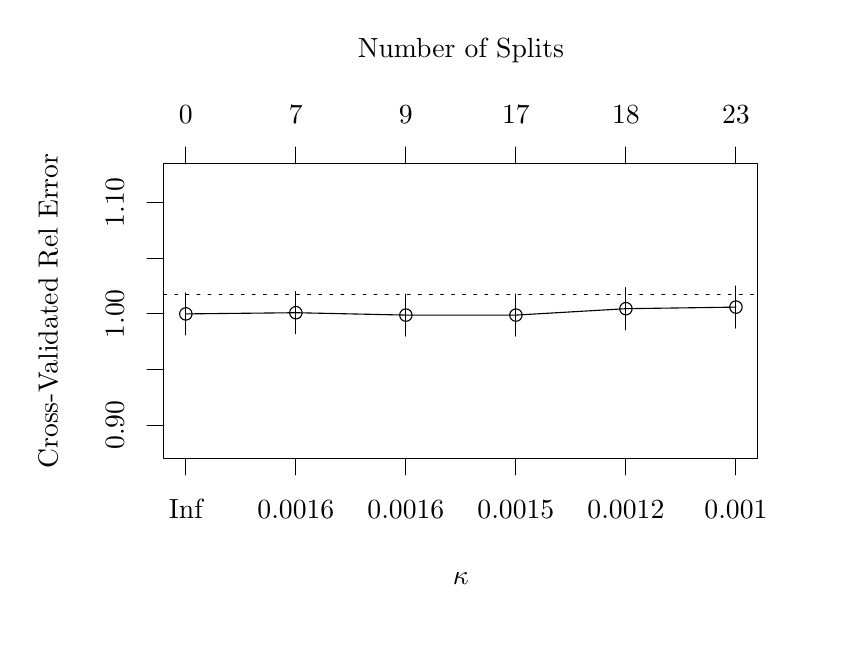
\begin{tikzpicture}[x=1pt,y=1pt]
\definecolor[named]{fillColor}{rgb}{1.00,1.00,1.00}
\path[use as bounding box,fill=fillColor,fill opacity=0.00] (0,0) rectangle (289.08,216.81);
\begin{scope}
\path[clip] ( 49.20, 61.20) rectangle (263.88,167.61);
\definecolor[named]{drawColor}{rgb}{0.00,0.00,0.00}

\path[draw=drawColor,line width= 0.4pt,line join=round,line cap=round] ( 57.15,113.38) --
	( 96.91,113.81) --
	(136.66,112.95) --
	(176.42,112.95) --
	(216.17,115.26) --
	(255.93,115.83);

\path[draw=drawColor,line width= 0.4pt,line join=round,line cap=round] ( 57.15,113.38) circle (  2.25);

\path[draw=drawColor,line width= 0.4pt,line join=round,line cap=round] ( 96.91,113.81) circle (  2.25);

\path[draw=drawColor,line width= 0.4pt,line join=round,line cap=round] (136.66,112.95) circle (  2.25);

\path[draw=drawColor,line width= 0.4pt,line join=round,line cap=round] (176.42,112.95) circle (  2.25);

\path[draw=drawColor,line width= 0.4pt,line join=round,line cap=round] (216.17,115.26) circle (  2.25);

\path[draw=drawColor,line width= 0.4pt,line join=round,line cap=round] (255.93,115.83) circle (  2.25);
\end{scope}
\begin{scope}
\path[clip] (  0.00,  0.00) rectangle (289.08,216.81);
\definecolor[named]{drawColor}{rgb}{0.00,0.00,0.00}

\node[text=drawColor,anchor=base,inner sep=0pt, outer sep=0pt, scale=  1.00] at (156.54, 15.60) {$\kappa$};

\node[text=drawColor,rotate= 90.00,anchor=base,inner sep=0pt, outer sep=0pt, scale=  1.00] at ( 10.80,114.40) {Cross-Validated Rel Error};
\end{scope}
\begin{scope}
\path[clip] (  0.00,  0.00) rectangle (289.08,216.81);
\definecolor[named]{drawColor}{rgb}{0.00,0.00,0.00}

\path[draw=drawColor,line width= 0.4pt,line join=round,line cap=round] ( 49.20, 61.20) --
	(263.88, 61.20) --
	(263.88,167.61) --
	( 49.20,167.61) --
	( 49.20, 61.20);

\path[draw=drawColor,line width= 0.4pt,line join=round,line cap=round] ( 49.20, 73.16) -- ( 49.20,153.60);

\path[draw=drawColor,line width= 0.4pt,line join=round,line cap=round] ( 49.20, 73.16) -- ( 43.20, 73.16);

\path[draw=drawColor,line width= 0.4pt,line join=round,line cap=round] ( 49.20, 93.27) -- ( 43.20, 93.27);

\path[draw=drawColor,line width= 0.4pt,line join=round,line cap=round] ( 49.20,113.38) -- ( 43.20,113.38);

\path[draw=drawColor,line width= 0.4pt,line join=round,line cap=round] ( 49.20,133.49) -- ( 43.20,133.49);

\path[draw=drawColor,line width= 0.4pt,line join=round,line cap=round] ( 49.20,153.60) -- ( 43.20,153.60);

\node[text=drawColor,rotate= 90.00,anchor=base,inner sep=0pt, outer sep=0pt, scale=  1.00] at ( 34.80, 73.16) {0.90};

\node[text=drawColor,rotate= 90.00,anchor=base,inner sep=0pt, outer sep=0pt, scale=  1.00] at ( 34.80,113.38) {1.00};

\node[text=drawColor,rotate= 90.00,anchor=base,inner sep=0pt, outer sep=0pt, scale=  1.00] at ( 34.80,153.60) {1.10};
\end{scope}
\begin{scope}
\path[clip] ( 49.20, 61.20) rectangle (263.88,167.61);
\definecolor[named]{drawColor}{rgb}{0.00,0.00,0.00}

\path[draw=drawColor,line width= 0.4pt,line join=round,line cap=round] ( 57.15,105.79) -- ( 57.15,120.97);

\path[draw=drawColor,line width= 0.4pt,line join=round,line cap=round] ( 96.91,106.22) -- ( 96.91,121.41);

\path[draw=drawColor,line width= 0.4pt,line join=round,line cap=round] (136.66,105.36) -- (136.66,120.53);

\path[draw=drawColor,line width= 0.4pt,line join=round,line cap=round] (176.42,105.36) -- (176.42,120.53);

\path[draw=drawColor,line width= 0.4pt,line join=round,line cap=round] (216.17,107.65) -- (216.17,122.87);

\path[draw=drawColor,line width= 0.4pt,line join=round,line cap=round] (255.93,108.22) -- (255.93,123.45);
\end{scope}
\begin{scope}
\path[clip] (  0.00,  0.00) rectangle (289.08,216.81);
\definecolor[named]{drawColor}{rgb}{0.00,0.00,0.00}

\path[draw=drawColor,line width= 0.4pt,line join=round,line cap=round] ( 57.15, 61.20) -- (255.93, 61.20);

\path[draw=drawColor,line width= 0.4pt,line join=round,line cap=round] ( 57.15, 61.20) -- ( 57.15, 55.20);

\path[draw=drawColor,line width= 0.4pt,line join=round,line cap=round] ( 96.91, 61.20) -- ( 96.91, 55.20);

\path[draw=drawColor,line width= 0.4pt,line join=round,line cap=round] (136.66, 61.20) -- (136.66, 55.20);

\path[draw=drawColor,line width= 0.4pt,line join=round,line cap=round] (176.42, 61.20) -- (176.42, 55.20);

\path[draw=drawColor,line width= 0.4pt,line join=round,line cap=round] (216.17, 61.20) -- (216.17, 55.20);

\path[draw=drawColor,line width= 0.4pt,line join=round,line cap=round] (255.93, 61.20) -- (255.93, 55.20);

\node[text=drawColor,anchor=base,inner sep=0pt, outer sep=0pt, scale=  1.00] at ( 57.15, 39.60) {Inf};

\node[text=drawColor,anchor=base,inner sep=0pt, outer sep=0pt, scale=  1.00] at ( 96.91, 39.60) {0.0016};

\node[text=drawColor,anchor=base,inner sep=0pt, outer sep=0pt, scale=  1.00] at (136.66, 39.60) {0.0016};

\node[text=drawColor,anchor=base,inner sep=0pt, outer sep=0pt, scale=  1.00] at (176.42, 39.60) {0.0015};

\node[text=drawColor,anchor=base,inner sep=0pt, outer sep=0pt, scale=  1.00] at (216.17, 39.60) {0.0012};

\node[text=drawColor,anchor=base,inner sep=0pt, outer sep=0pt, scale=  1.00] at (255.93, 39.60) {0.001};

\path[draw=drawColor,line width= 0.4pt,line join=round,line cap=round] ( 57.15,167.61) -- (255.93,167.61);

\path[draw=drawColor,line width= 0.4pt,line join=round,line cap=round] ( 57.15,167.61) -- ( 57.15,173.61);

\path[draw=drawColor,line width= 0.4pt,line join=round,line cap=round] ( 96.91,167.61) -- ( 96.91,173.61);

\path[draw=drawColor,line width= 0.4pt,line join=round,line cap=round] (136.66,167.61) -- (136.66,173.61);

\path[draw=drawColor,line width= 0.4pt,line join=round,line cap=round] (176.42,167.61) -- (176.42,173.61);

\path[draw=drawColor,line width= 0.4pt,line join=round,line cap=round] (216.17,167.61) -- (216.17,173.61);

\path[draw=drawColor,line width= 0.4pt,line join=round,line cap=round] (255.93,167.61) -- (255.93,173.61);

\node[text=drawColor,anchor=base,inner sep=0pt, outer sep=0pt, scale=  1.00] at ( 57.15,182.01) {0};

\node[text=drawColor,anchor=base,inner sep=0pt, outer sep=0pt, scale=  1.00] at ( 96.91,182.01) {7};

\node[text=drawColor,anchor=base,inner sep=0pt, outer sep=0pt, scale=  1.00] at (136.66,182.01) {9};

\node[text=drawColor,anchor=base,inner sep=0pt, outer sep=0pt, scale=  1.00] at (176.42,182.01) {17};

\node[text=drawColor,anchor=base,inner sep=0pt, outer sep=0pt, scale=  1.00] at (216.17,182.01) {18};

\node[text=drawColor,anchor=base,inner sep=0pt, outer sep=0pt, scale=  1.00] at (255.93,182.01) {23};

\node[text=drawColor,anchor=base,inner sep=0pt, outer sep=0pt, scale=  1.00] at (156.54,206.01) {Number of Splits};
\end{scope}
\begin{scope}
\path[clip] ( 49.20, 61.20) rectangle (263.88,167.61);
\definecolor[named]{drawColor}{rgb}{0.00,0.00,0.00}

\path[draw=drawColor,line width= 0.4pt,dash pattern=on 1pt off 3pt ,line join=round,line cap=round] ( 49.20,120.53) -- (263.88,120.53);
\end{scope}
\end{tikzpicture}

  \end{center}

  \vspace{-0.3in}

  This value was used to prune the tree shown below. The leaves of the tree are shaded according to whether war (MID hostilities $\geq$ 4 ) or peace is more likely, and the value at each leaf indicates the relative frequency of war in the training set. 

\vspace{-1.3in}
  \begin{center}
    % Created by tikzDevice version 0.6.4 on 2013-12-01 11:37:16
% !TEX encoding = UTF-8 Unicode
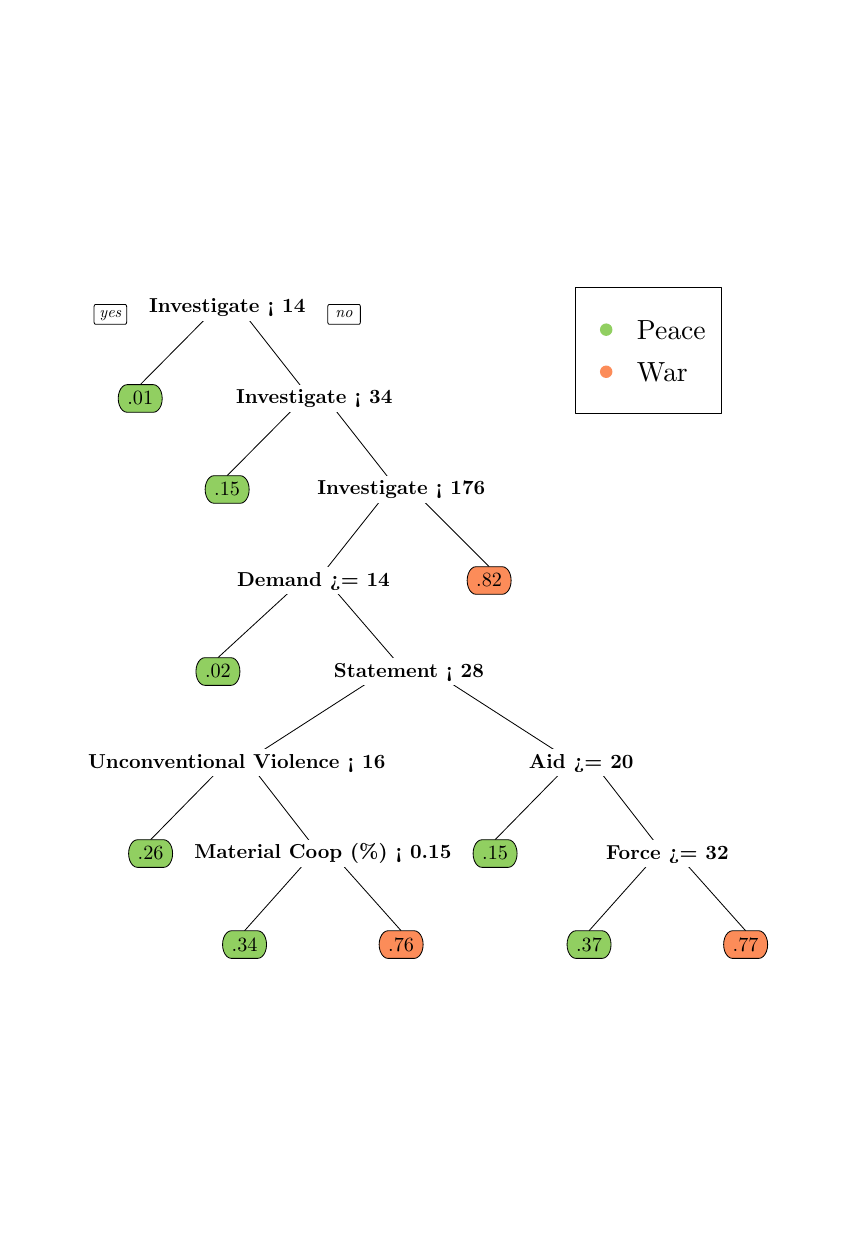
\begin{tikzpicture}[x=1pt,y=1pt]
\definecolor[named]{fillColor}{rgb}{1.00,1.00,1.00}
\path[use as bounding box,fill=fillColor,fill opacity=0.00] (0,0) rectangle (289.08,433.62);
\begin{scope}
\path[clip] (  0.00,  0.00) rectangle (289.08,433.62);
\definecolor[named]{drawColor}{rgb}{0.00,0.00,0.00}

\path[draw=drawColor,line width= 0.3pt,line join=round] ( 40.67,304.62) --
	( 65.82,330.02) --
	( 72.11,330.02);

\path[draw=drawColor,line width= 0.3pt,line join=round] (103.54,297.96) --
	( 78.39,330.02) --
	( 72.11,330.02);

\path[draw=drawColor,line width= 0.3pt,line join=round] ( 72.08,271.73) --
	( 97.25,297.13) --
	(103.54,297.13);

\path[draw=drawColor,line width= 0.3pt,line join=round] (135.01,265.07) --
	(109.84,297.13) --
	(103.54,297.13);

\path[draw=drawColor,line width= 0.3pt,line join=round] (103.27,232.19) --
	(128.66,264.24) --
	(135.01,264.24);

\path[draw=drawColor,line width= 0.3pt,line join=round] ( 68.75,205.96) --
	( 96.36,231.35) --
	(103.27,231.35);

\path[draw=drawColor,line width= 0.3pt,line join=round] (137.78,199.30) --
	(110.17,231.35) --
	(103.27,231.35);

\path[draw=drawColor,line width= 0.3pt,line join=round] ( 75.54,166.41) --
	(125.33,198.47) --
	(137.78,198.47);

\path[draw=drawColor,line width= 0.3pt,line join=round] ( 44.42,140.18) --
	( 69.32,165.58) --
	( 75.54,165.58);

\path[draw=drawColor,line width= 0.3pt,line join=round] (106.66,133.52) --
	( 81.76,165.58) --
	( 75.54,165.58);

\path[draw=drawColor,line width= 0.3pt,line join=round] ( 78.37,107.29) --
	(101.00,132.69) --
	(106.66,132.69);

\path[draw=drawColor,line width= 0.3pt,line join=round] (134.95,107.29) --
	(112.32,132.69) --
	(106.66,132.69);

\path[draw=drawColor,line width= 0.3pt,line join=round] (200.02,166.41) --
	(150.23,198.47) --
	(137.78,198.47);

\path[draw=drawColor,line width= 0.3pt,line join=round] (168.90,140.18) --
	(193.80,165.58) --
	(200.02,165.58);

\path[draw=drawColor,line width= 0.3pt,line join=round] (231.14,133.52) --
	(206.25,165.58) --
	(200.02,165.58);

\path[draw=drawColor,line width= 0.3pt,line join=round] (202.85,107.29) --
	(225.48,132.69) --
	(231.14,132.69);

\path[draw=drawColor,line width= 0.3pt,line join=round] (259.43,107.29) --
	(236.80,132.69) --
	(231.14,132.69);

\path[draw=drawColor,line width= 0.3pt,line join=round] (166.75,238.84) --
	(141.36,264.24) --
	(135.01,264.24);
\definecolor[named]{fillColor}{rgb}{1.00,1.00,1.00}

\path[fill=fillColor] ( 38.12,327.52) --
	( 38.12,337.52) --
	(106.09,337.52) --
	(106.09,327.52) --
	( 38.12,327.52) --
	cycle;

\path[fill=fillColor] ( 69.56,294.63) --
	( 69.56,304.64) --
	(137.52,304.64) --
	(137.52,294.63) --
	( 69.56,294.63) --
	cycle;

\path[fill=fillColor] ( 98.94,261.74) --
	( 98.94,271.75) --
	(171.07,271.75) --
	(171.07,261.74) --
	( 98.94,261.74) --
	cycle;

\path[fill=fillColor] ( 70.64,228.85) --
	( 70.64,238.86) --
	(135.89,238.86) --
	(135.89,228.85) --
	( 70.64,228.85) --
	cycle;

\path[fill=fillColor] (104.94,195.96) --
	(104.94,205.97) --
	(170.62,205.97) --
	(170.62,195.96) --
	(104.94,195.96) --
	cycle;

\path[fill=fillColor] ( 16.26,163.08) --
	( 16.26,173.08) --
	(134.83,173.08) --
	(134.83,163.08) --
	( 16.26,163.08) --
	cycle;

\path[fill=fillColor] ( 54.60,130.19) --
	( 54.60,140.19) --
	(158.72,140.19) --
	(158.72,130.19) --
	( 54.60,130.19) --
	cycle;

\path[fill=fillColor] (176.01,163.08) --
	(176.01,173.08) --
	(224.03,173.08) --
	(224.03,163.08) --
	(176.01,163.08) --
	cycle;

\path[fill=fillColor] (203.92,130.19) --
	(203.92,140.19) --
	(258.37,140.19) --
	(258.37,130.19) --
	(203.92,130.19) --
	cycle;

\node[text=drawColor,anchor=base,inner sep=0pt, outer sep=0pt, scale=  0.73] at ( 72.11,330.72) {\bfseries Investigate < 14};

\node[text=drawColor,anchor=base,inner sep=0pt, outer sep=0pt, scale=  0.73] at (103.54,297.84) {\bfseries Investigate < 34};

\node[text=drawColor,anchor=base,inner sep=0pt, outer sep=0pt, scale=  0.73] at (135.01,264.95) {\bfseries Investigate < 176};

\node[text=drawColor,anchor=base,inner sep=0pt, outer sep=0pt, scale=  0.73] at (103.27,231.71) {\bfseries Demand >= 14};

\node[text=drawColor,anchor=base,inner sep=0pt, outer sep=0pt, scale=  0.73] at (137.78,198.82) {\bfseries Statement < 28};

\node[text=drawColor,anchor=base,inner sep=0pt, outer sep=0pt, scale=  0.73] at ( 75.54,165.93) {\bfseries Unconventional Violence < 16};

\node[text=drawColor,anchor=base,inner sep=0pt, outer sep=0pt, scale=  0.73] at (106.66,133.38) {\bfseries Material Coop (\%) < 0.15};

\node[text=drawColor,anchor=base,inner sep=0pt, outer sep=0pt, scale=  0.73] at (200.02,165.93) {\bfseries Aid >= 20};

\node[text=drawColor,anchor=base,inner sep=0pt, outer sep=0pt, scale=  0.73] at (231.14,133.04) {\bfseries Force >= 32};
\definecolor[named]{fillColor}{rgb}{0.57,0.81,0.38}

\path[draw=drawColor,line width= 0.3pt,line join=round,line cap=round,fill=fillColor] ( 32.71,299.63) --
	( 32.82,300.92) --
	( 33.15,302.12) --
	( 33.66,303.16) --
	( 34.33,303.95) --
	( 35.11,304.45) --
	( 35.95,304.62) --
	( 45.39,304.62) --
	( 46.23,304.45) --
	( 47.00,303.95) --
	( 47.67,303.16) --
	( 48.19,302.12) --
	( 48.51,300.92) --
	( 48.62,299.63) --
	( 48.62,299.63) --
	( 48.51,298.34) --
	( 48.19,297.13) --
	( 47.67,296.10) --
	( 47.00,295.30) --
	( 46.23,294.80) --
	( 45.39,294.63) --
	( 35.95,294.63) --
	( 35.11,294.80) --
	( 34.33,295.30) --
	( 33.66,296.10) --
	( 33.15,297.13) --
	( 32.82,298.34) --
	( 32.71,299.63) --
	cycle;

\path[draw=drawColor,line width= 0.3pt,line join=round,line cap=round,fill=fillColor] ( 64.12,266.74) --
	( 64.23,268.03) --
	( 64.56,269.24) --
	( 65.07,270.27) --
	( 65.74,271.06) --
	( 66.52,271.56) --
	( 67.36,271.73) --
	( 76.80,271.73) --
	( 77.64,271.56) --
	( 78.41,271.06) --
	( 79.08,270.27) --
	( 79.60,269.24) --
	( 79.92,268.03) --
	( 80.03,266.74) --
	( 80.03,266.74) --
	( 79.92,265.45) --
	( 79.60,264.24) --
	( 79.08,263.21) --
	( 78.41,262.42) --
	( 77.64,261.92) --
	( 76.80,261.75) --
	( 67.36,261.75) --
	( 66.52,261.92) --
	( 65.74,262.42) --
	( 65.07,263.21) --
	( 64.56,264.24) --
	( 64.23,265.45) --
	( 64.12,266.74) --
	cycle;

\path[draw=drawColor,line width= 0.3pt,line join=round,line cap=round,fill=fillColor] ( 60.80,200.96) --
	( 60.91,202.26) --
	( 61.23,203.46) --
	( 61.74,204.49) --
	( 62.41,205.29) --
	( 63.19,205.79) --
	( 64.03,205.96) --
	( 73.47,205.96) --
	( 74.31,205.79) --
	( 75.09,205.29) --
	( 75.76,204.49) --
	( 76.27,203.46) --
	( 76.59,202.26) --
	( 76.70,200.96) --
	( 76.70,200.96) --
	( 76.59,199.67) --
	( 76.27,198.47) --
	( 75.76,197.43) --
	( 75.09,196.64) --
	( 74.31,196.14) --
	( 73.47,195.97) --
	( 64.03,195.97) --
	( 63.19,196.14) --
	( 62.41,196.64) --
	( 61.74,197.43) --
	( 61.23,198.47) --
	( 60.91,199.67) --
	( 60.80,200.96) --
	cycle;

\path[draw=drawColor,line width= 0.3pt,line join=round,line cap=round,fill=fillColor] ( 36.47,135.19) --
	( 36.58,136.48) --
	( 36.90,137.68) --
	( 37.41,138.72) --
	( 38.08,139.51) --
	( 38.86,140.01) --
	( 39.70,140.18) --
	( 49.14,140.18) --
	( 49.98,140.01) --
	( 50.76,139.51) --
	( 51.43,138.72) --
	( 51.94,137.68) --
	( 52.26,136.48) --
	( 52.37,135.19) --
	( 52.37,135.19) --
	( 52.26,133.89) --
	( 51.94,132.69) --
	( 51.43,131.66) --
	( 50.76,130.86) --
	( 49.98,130.36) --
	( 49.14,130.19) --
	( 39.70,130.19) --
	( 38.86,130.36) --
	( 38.08,130.86) --
	( 37.41,131.66) --
	( 36.90,132.69) --
	( 36.58,133.89) --
	( 36.47,135.19) --
	cycle;

\path[draw=drawColor,line width= 0.3pt,line join=round,line cap=round,fill=fillColor] ( 70.42,102.30) --
	( 70.53,103.59) --
	( 70.85,104.79) --
	( 71.36,105.83) --
	( 72.03,106.62) --
	( 72.81,107.12) --
	( 73.65,107.29) --
	( 83.09,107.29) --
	( 83.93,107.12) --
	( 84.71,106.62) --
	( 85.38,105.83) --
	( 85.89,104.79) --
	( 86.21,103.59) --
	( 86.32,102.30) --
	( 86.32,102.30) --
	( 86.21,101.01) --
	( 85.89, 99.80) --
	( 85.38, 98.77) --
	( 84.71, 97.97) --
	( 83.93, 97.47) --
	( 83.09, 97.30) --
	( 73.65, 97.30) --
	( 72.81, 97.47) --
	( 72.03, 97.97) --
	( 71.36, 98.77) --
	( 70.85, 99.80) --
	( 70.53,101.01) --
	( 70.42,102.30) --
	cycle;
\definecolor[named]{fillColor}{rgb}{0.99,0.55,0.35}

\path[draw=drawColor,line width= 0.3pt,line join=round,line cap=round,fill=fillColor] (127.00,102.30) --
	(127.11,103.59) --
	(127.43,104.79) --
	(127.95,105.83) --
	(128.61,106.62) --
	(129.39,107.12) --
	(130.23,107.29) --
	(139.67,107.29) --
	(140.51,107.12) --
	(141.29,106.62) --
	(141.96,105.83) --
	(142.47,104.79) --
	(142.79,103.59) --
	(142.90,102.30) --
	(142.90,102.30) --
	(142.79,101.01) --
	(142.47, 99.80) --
	(141.96, 98.77) --
	(141.29, 97.97) --
	(140.51, 97.47) --
	(139.67, 97.30) --
	(130.23, 97.30) --
	(129.39, 97.47) --
	(128.61, 97.97) --
	(127.95, 98.77) --
	(127.43, 99.80) --
	(127.11,101.01) --
	(127.00,102.30) --
	cycle;
\definecolor[named]{fillColor}{rgb}{0.57,0.81,0.38}

\path[draw=drawColor,line width= 0.3pt,line join=round,line cap=round,fill=fillColor] (160.95,135.19) --
	(161.06,136.48) --
	(161.38,137.68) --
	(161.89,138.72) --
	(162.56,139.51) --
	(163.34,140.01) --
	(164.18,140.18) --
	(173.62,140.18) --
	(174.46,140.01) --
	(175.24,139.51) --
	(175.91,138.72) --
	(176.42,137.68) --
	(176.74,136.48) --
	(176.85,135.19) --
	(176.85,135.19) --
	(176.74,133.89) --
	(176.42,132.69) --
	(175.91,131.66) --
	(175.24,130.86) --
	(174.46,130.36) --
	(173.62,130.19) --
	(164.18,130.19) --
	(163.34,130.36) --
	(162.56,130.86) --
	(161.89,131.66) --
	(161.38,132.69) --
	(161.06,133.89) --
	(160.95,135.19) --
	cycle;

\path[draw=drawColor,line width= 0.3pt,line join=round,line cap=round,fill=fillColor] (194.90,102.30) --
	(195.01,103.59) --
	(195.33,104.79) --
	(195.84,105.83) --
	(196.51,106.62) --
	(197.29,107.12) --
	(198.13,107.29) --
	(207.57,107.29) --
	(208.41,107.12) --
	(209.19,106.62) --
	(209.86,105.83) --
	(210.37,104.79) --
	(210.69,103.59) --
	(210.80,102.30) --
	(210.80,102.30) --
	(210.69,101.01) --
	(210.37, 99.80) --
	(209.86, 98.77) --
	(209.19, 97.97) --
	(208.41, 97.47) --
	(207.57, 97.30) --
	(198.13, 97.30) --
	(197.29, 97.47) --
	(196.51, 97.97) --
	(195.84, 98.77) --
	(195.33, 99.80) --
	(195.01,101.01) --
	(194.90,102.30) --
	cycle;
\definecolor[named]{fillColor}{rgb}{0.99,0.55,0.35}

\path[draw=drawColor,line width= 0.3pt,line join=round,line cap=round,fill=fillColor] (251.48,102.30) --
	(251.59,103.59) --
	(251.91,104.79) --
	(252.43,105.83) --
	(253.10,106.62) --
	(253.88,107.12) --
	(254.71,107.29) --
	(264.16,107.29) --
	(264.99,107.12) --
	(265.77,106.62) --
	(266.44,105.83) --
	(266.95,104.79) --
	(267.28,103.59) --
	(267.39,102.30) --
	(267.39,102.30) --
	(267.28,101.01) --
	(266.95, 99.80) --
	(266.44, 98.77) --
	(265.77, 97.97) --
	(264.99, 97.47) --
	(264.16, 97.30) --
	(254.71, 97.30) --
	(253.88, 97.47) --
	(253.10, 97.97) --
	(252.43, 98.77) --
	(251.91, 99.80) --
	(251.59,101.01) --
	(251.48,102.30) --
	cycle;

\path[draw=drawColor,line width= 0.3pt,line join=round,line cap=round,fill=fillColor] (158.80,233.85) --
	(158.91,235.14) --
	(159.23,236.35) --
	(159.74,237.38) --
	(160.41,238.18) --
	(161.19,238.67) --
	(162.03,238.84) --
	(171.47,238.84) --
	(172.31,238.67) --
	(173.09,238.18) --
	(173.76,237.38) --
	(174.27,236.35) --
	(174.59,235.14) --
	(174.70,233.85) --
	(174.70,233.85) --
	(174.59,232.56) --
	(174.27,231.35) --
	(173.76,230.32) --
	(173.09,229.53) --
	(172.31,229.03) --
	(171.47,228.86) --
	(162.03,228.86) --
	(161.19,229.03) --
	(160.41,229.53) --
	(159.74,230.32) --
	(159.23,231.35) --
	(158.91,232.56) --
	(158.80,233.85) --
	cycle;

\node[text=drawColor,anchor=base,inner sep=0pt, outer sep=0pt, scale=  0.73] at ( 40.67,297.30) {.01};

\node[text=drawColor,anchor=base,inner sep=0pt, outer sep=0pt, scale=  0.73] at ( 72.08,264.41) {.15};

\node[text=drawColor,anchor=base,inner sep=0pt, outer sep=0pt, scale=  0.73] at ( 68.75,198.64) {.02};

\node[text=drawColor,anchor=base,inner sep=0pt, outer sep=0pt, scale=  0.73] at ( 44.42,132.86) {.26};

\node[text=drawColor,anchor=base,inner sep=0pt, outer sep=0pt, scale=  0.73] at ( 78.37, 99.97) {.34};

\node[text=drawColor,anchor=base,inner sep=0pt, outer sep=0pt, scale=  0.73] at (134.95, 99.97) {.76};

\node[text=drawColor,anchor=base,inner sep=0pt, outer sep=0pt, scale=  0.73] at (168.90,132.86) {.15};

\node[text=drawColor,anchor=base,inner sep=0pt, outer sep=0pt, scale=  0.73] at (202.85, 99.97) {.37};

\node[text=drawColor,anchor=base,inner sep=0pt, outer sep=0pt, scale=  0.73] at (259.43, 99.97) {.77};

\node[text=drawColor,anchor=base,inner sep=0pt, outer sep=0pt, scale=  0.73] at (166.75,231.53) {.82};
\definecolor[named]{fillColor}{rgb}{1.00,1.00,1.00}

\path[draw=drawColor,line width= 0.3pt,line join=round,line cap=round,fill=fillColor] ( 23.99,332.72) --
	( 24.01,332.95) --
	( 24.06,333.17) --
	( 24.16,333.35) --
	( 24.28,333.49) --
	( 24.42,333.58) --
	( 24.57,333.61) --
	( 35.19,333.61) --
	( 35.34,333.58) --
	( 35.48,333.49) --
	( 35.60,333.35) --
	( 35.69,333.17) --
	( 35.75,332.95) --
	( 35.77,332.72) --
	( 35.77,327.32) --
	( 35.75,327.09) --
	( 35.69,326.87) --
	( 35.60,326.69) --
	( 35.48,326.54) --
	( 35.34,326.46) --
	( 35.19,326.42) --
	( 24.57,326.42) --
	( 24.42,326.46) --
	( 24.28,326.54) --
	( 24.16,326.69) --
	( 24.06,326.87) --
	( 24.01,327.09) --
	( 23.99,327.32) --
	cycle;

\path[draw=drawColor,line width= 0.3pt,line join=round,line cap=round,fill=fillColor] (108.44,332.72) --
	(108.46,332.95) --
	(108.52,333.17) --
	(108.61,333.35) --
	(108.73,333.49) --
	(108.87,333.58) --
	(109.02,333.61) --
	(119.64,333.61) --
	(119.79,333.58) --
	(119.93,333.49) --
	(120.05,333.35) --
	(120.15,333.17) --
	(120.20,332.95) --
	(120.22,332.72) --
	(120.22,327.32) --
	(120.20,327.09) --
	(120.15,326.87) --
	(120.05,326.69) --
	(119.93,326.54) --
	(119.79,326.46) --
	(119.64,326.42) --
	(109.02,326.42) --
	(108.87,326.46) --
	(108.73,326.54) --
	(108.61,326.69) --
	(108.52,326.87) --
	(108.46,327.09) --
	(108.44,327.32) --
	cycle;

\node[text=drawColor,anchor=base,inner sep=0pt, outer sep=0pt, scale=  0.58] at ( 29.88,328.74) {\itshape yes};

\node[text=drawColor,anchor=base,inner sep=0pt, outer sep=0pt, scale=  0.58] at (114.33,328.77) {\itshape no};
\end{scope}
\begin{scope}
\path[clip] ( 49.20, 61.20) rectangle (263.88,384.42);
\definecolor[named]{drawColor}{rgb}{0.00,0.00,0.00}

\path[draw=drawColor,line width= 0.4pt,line join=round,line cap=round] (197.93,339.70) rectangle (250.57,294.07);
\definecolor[named]{fillColor}{rgb}{0.57,0.81,0.38}

\path[fill=fillColor] (209.05,324.49) circle (  2.25);
\definecolor[named]{fillColor}{rgb}{0.99,0.55,0.35}

\path[fill=fillColor] (209.05,309.28) circle (  2.25);

\node[text=drawColor,anchor=base west,inner sep=0pt, outer sep=0pt, scale=  1.00] at (220.16,321.04) {Peace};

\node[text=drawColor,anchor=base west,inner sep=0pt, outer sep=0pt, scale=  1.00] at (220.16,305.84) {War};
\end{scope}
\end{tikzpicture}

  \end{center}
  
\vspace{-1.3in}
  The table below presents several measures of accuracy for the classification tree compared to a null model (all predicted values are zero) and a logistic regression model using the same features. The test set covers 1992-1998 (\emph{n}=372,271) and the training set covers 1999-2001 (\emph{n}=213,218). The classification tree outperforms the other two models in all respects for the training data, and in most respects for the test data. 

  \begin{center}
  \begin{tabular}{l|ccc|ccc}
   \multicolumn{1}{c}{} & \multicolumn{3}{c}{Training Data} & \multicolumn{3}{c}{Test Data} \\
  Model & MSE & Precision & Recall & MSE & Precision & Recall \\
  \midrule
  Null & 0.0075 & 0.000 & 0.000 & 0.0066 & 0.000 & 0.000 \\
  GLM & 0.0082 & 0.158 & 0.022  & 0.0079 & 0.142 & 0.038 \\
  CART & 0.0067 & 0.702 & 0.192 & 0.0066 & 0.422 & 0.027 
  \end{tabular}
  \end{center}
 }


%%%%%%
  \headerbox{\bf Results}{name=predictions,column=2,row=0}{
%%%%%
  
    \begin{center}
      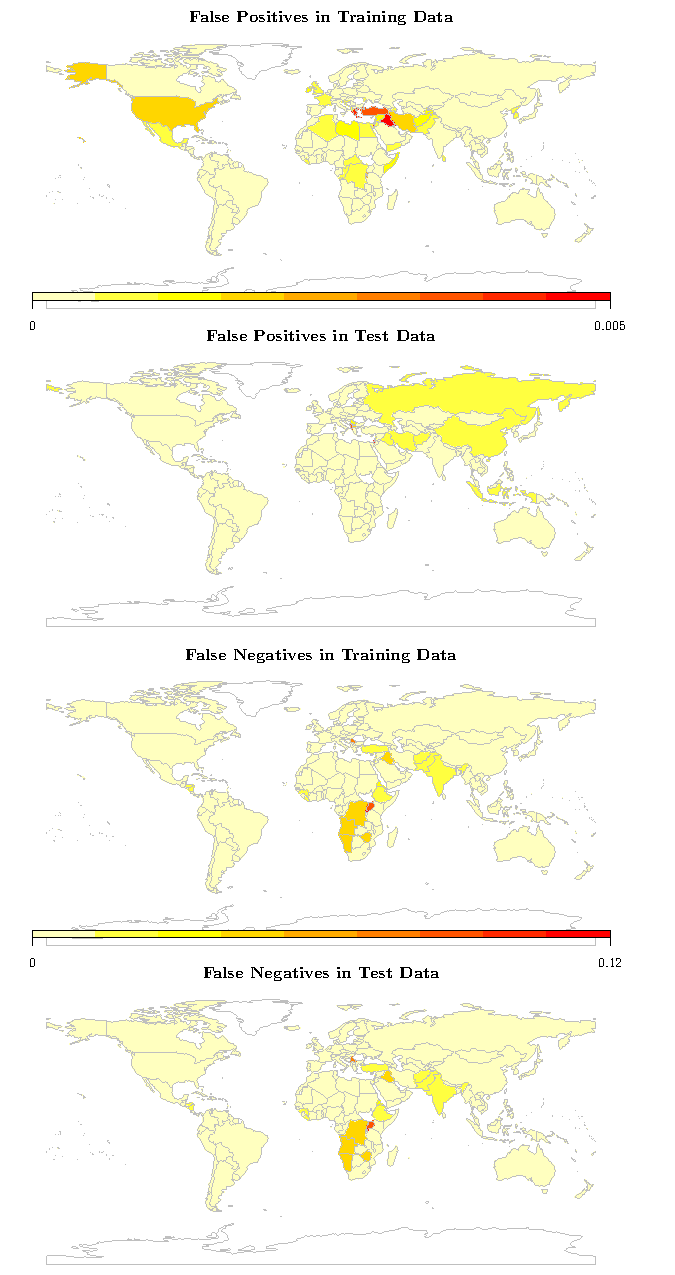
\includegraphics{../graphics/diagnostics.pdf}
    \end{center}

 }

%%%%%%
  \headerbox{\bf Outlook}{name=conclusion,below=predictions,above=bottom,column=2}{
%%%%%
   \begin{itemize} \compresslist
      \item CART handles interactions between features better than GLM.
      \item Next steps include SMOTE for rare events, using spatial and network lags to account for interdependence between countries, and a comparison to random forest.
      \item More advanced methods and a final pass by human coders will likely be required to obtain fully accurate classifications.
      \item Automated methods can offer a quick and inexpensive first approximation of political indicators.
  \end{itemize}
 }

\end{poster}
\end{document}